% define the document class as a report.
\documentclass[letterpaper]{report}

% include a metric crap-tonne of latex packages. the most important bit here
% is the metadata specified during loading the hyperref package. you'll want
% to change the pdfauthor and pdftitle fields to suit your purposes.
\usepackage{float}
\usepackage{array}
\usepackage{amsmath}
\usepackage{amsfonts}
\usepackage{setspace}
\usepackage{chapterbib}
\usepackage{natbib}
\usepackage{bibentry}
\usepackage[
  pdftex,
  pdfauthor={Bradley Worley},
  pdftitle={Chemometric and Bioinformatic Analyses of Cellular Biochemistry},
  hidelinks]{hyperref}
\usepackage{etoolbox}
\usepackage{graphicx}
\usepackage{setspace}
\usepackage{adjustbox}
\usepackage[labelfont=bf]{caption}
\usepackage{sidecap}
\usepackage[chapter]{algorithm}
\usepackage{algorithmic}

% reference sections are typically un-numbered chapter headings, which don't
% work with what we need to do in the thesis. this changes the bibliography
% into a numbered section heading with the title `References'.
\renewcommand\bibsection{%
 \section{References}%
 \markboth{\MakeUppercase{\refname}}{\MakeUppercase{\refname}}%
}%

% the algorithmic package doesn't quite have what we want, so these commands
% change the \REQUIRE and \ENSURE commands into 'Inputs' and 'Outputs',
% respectively.
\renewcommand{\algorithmicrequire}{\textbf{Input:}}
\renewcommand{\algorithmicensure}{\textbf{Output:}}

% define the margins and turn off indentation.
\setlength{\textwidth}{6.5in}
\setlength{\textheight}{9in}
\setlength{\oddsidemargin}{0in}
\setlength{\topmargin}{-.5in}
\setlength{\parindent}{0em}

% math operators require a different definition from regular tex commands.
\DeclareMathOperator*{\argmin}{\arg\!\min}

% define a bunch of shortcuts for denoting nmr-active nuclides, as well
% as pairs of nuclides used in correlation spectroscopy.
\newcommand{\hnmr}{$^{1}$H}
\newcommand{\dnmr}{$^{2}$H}
\newcommand{\cnmr}{$^{13}$C}
\newcommand{\nnmr}{$^{15}$N}
\newcommand{\onmr}{$^{17}$O}
\newcommand{\fnmr}{$^{19}$F}
\newcommand{\pnmr}{$^{31}$P}
\newcommand{\hhnmr}{$^{1}$H--$^{1}$H}
\newcommand{\hcnmr}{$^{1}$H--$^{13}$C}
\newcommand{\hnnmr}{$^{1}$H--$^{15}$N}

% define a few shorthands (for using inside equation and align environments)
% for sums of squares and squared frobenius norms.
\newcommand{\ssfit}{SS_{\mathrm{fit}}}
\newcommand{\sserr}{SS_{\mathrm{err}}}
\newcommand{\sstot}{SS_{\mathrm{total}}}
\newcommand{\frosq}[1]{\left\| #1 \right\|_F^2}
\newcommand{\ints}[2]{\mathbb{Z}_{#1}^{#2}}

% define a few of the commonly used statistics generated from internally
% cross-validating bilinear matrix factorizations.
\newcommand{\rsq}{$R^2$}
\newcommand{\rsqx}{$R^2_X$}
\newcommand{\rsqy}{$R^2_Y$}
\newcommand{\rsqxp}{$R^2_{X,p}$}
\newcommand{\rsqxo}{$R^2_{X,o}$}
\newcommand{\qsq}{$Q^2$}

% define a few shortcuts for molecular orbital transitions and interactions.
\newcommand{\nnstar}{$n - n^\ast$}
\newcommand{\npistar}{$n - \pi^\ast$}
\newcommand{\nspistar}{$n_\sigma - \pi^\ast$}
\newcommand{\npipistar}{$n_\pi - \pi^\ast$}
\newcommand{\pipistar}{$\pi - \pi^\ast$}
\newcommand{\pistar}{$\pi^\ast$}

% define a new command and tabular column type to rotate text ninety
% degrees counterclockwise inside table environments.
\newcolumntype{R}[2]{%
    >{\adjustbox{angle=#1,lap=\width-(#2)}\bgroup}%
    l%
    <{\egroup}%
}
\newcommand*\rot{\multicolumn{1}{R{90}{1em}}}

% big bang.
\begin{document}

% a bunch of anal-retentive exact spacing follows from here.
\begin{titlepage}
\begin{center}

% write a big, impressive title with big, impressive words.
\textbf{
  \huge Chemometric and Bioinformatic Analyses of Cellular Biochemistry
}
\\[20pt]

% you should put your name here instead of mine.
\emph{By} \\[12pt] {\large Bradley Worley} \\[40pt]

% no shit, sherlock.
\textsc{A Doctoral Dissertation} \\[40pt]

% more obvious things.
Submitted to the faculty of the Graduate College \\
at the University of Nebraska in partial fulfillment \\
of requirements for the degree of Doctor of Philosophy
\\[80pt]

% i'm still shocked that i'm getting a degree in chemistry...
\textsc{Major:}
\emph{Chemistry} \\[20pt]

% yup, the boss man.
\textsc{Supervisor:}
\emph{Professor Robert Powers} \\[20pt]

% it all happened here.
Lincoln, Nebraska \\
{\large \today}
\\[180pt]

% damn right! but change the notice for your thesis.
Copyright \copyright{} 2015 Bradley Worley

% unless you want to give my gramps a dedication, maybe change this
% to what you want to say?
\clearpage
\thispagestyle{empty}
\emph{
  \large For Wendell B. Worley. \\
  I hope you have PDF viewers in heaven, \\
  because you'd really love reading this. \\
}

% oh thank god, the anal-rententiveness is finally over.
\end{center}
\end{titlepage}

% source in the abstract and acknowledgements as if they were just written
% here, in this file... but use some special wizardry to include the
% list of publications. shh.... don't ask why.

\begin{abstract}
\begin{doublespace}
The amount of information collected and analyzed in biochemical and
bioanalytical research has exploded over the last few decades, due in large
part to the increasing availability of analytical intrumentation that yields
information-rich spectra. Datasets from Nuclear Magnetic Resonance (NMR),
Mass Spectrometry (MS), infrared (IR) or Raman spectroscopy may easily carry
tens to hundreds of thousands of potentially correlated variables observed
from only a few samples, making the application of classical statistical
methods inappropriate, if not impossible. Drawing useful biochemical
conclusions from these unique sources of data requires the use of specialized
multivariate data handling techniques.
\\\\
Unfortunately, proper implementation of many new multivariate algorithms
requires domain knowledge in mathematics, statistics, digital signal
processing, and software engineering {\it in addition to} analytical chemical
and biochemical expertise. As a consequence, analysts using multivariate
statistical methods were routinely required to chain together multiple
commercial software packages and fashion small ad hoc software solutions
to interpret a single dataset. This has been especially true in the field of
NMR metabolomics, where no single software package, free or otherwise, was
capable of completing all operations required to transform raw instrumental
data into a set of validated, informative multivariate models. Therefore,
while many powerful methods exist in published literature to statistically
treat and model multivariate spectral data, few are readily available for
immediate use by the community as a whole.
\\\\
This dissertation describes the development of an end-to-end software solution
for the handling and multivariate statistical modeling of spectroscopic data,
called MVAPACK, and a set of novel spectral data acquisition, processing and
treatment algorithms whose creation was expedited by MVAPACK. A final foray
into the potential existence of \npistar{} interactions within proteins is
also presented.
\end{doublespace}
\end{abstract}



\bibliographystyle{abbrv}
\nobibliography{bworley}

\renewcommand{\abstractname}{Acknowledgements}
\begin{abstract}
\begin{doublespace}
First and undeniably foremost, I extend my heartfelt gratitude to my family,
whose encouragement and words of wisdom and guidance were arguably the most
important contributor to my success in graduate school. Mom and Dad, you also
sparked my scientific curiosity from a young age, and introduced me to so
many scientific and intellectual opportunities. Elyssa, your encouragement
and humor were always a much-needed reminder that light actually existed at
the end of the tunnel I was passing through. I'm so proud of you, and I'm glad
I have you as my sister.
\\\\
Of course, no mention of family would be complete without my colleagues and
mentors I had the privilege of working with on a daily basis. I'm happy the
pressure cooker of graduate school brought us all closer than any ordinary
coworkers. Dr. Martha Morton, your honest, uncensored insights on academic
research, analytical chemical instrumentation and human interaction were
always a pleasure to receive and will remain an invaluable aid in whatever
future I choose to pursue. To Matt Shortridge, Jaime Stark, Jenni Copeland,
Bo Zhang, Steve Halouska, Teklab Gebregiworgis, Darrell Marshall, Shulei Lei
and Jonathan Catazaro, I'm thankful for the opportunities I had to share
everything from scientific results to burdens of conscience with you. I
would not have chosen to endure the rigours of graduate school if it were
not for all of you. To the current Powers group, I challenge you to keep
our truly remarkable comradery alive as the next round of junior students
enters our clan. I have undoubtedly learned the most from all of you, and
I hope those who join us next will share in that truly sustaining
collaborative, friendly atmosphere that the Powers group thrives upon.
\\\\
Finally, I wish to sincerely thank my advisor, Dr. Robert Powers, and the
members of my supervisory committee, Drs. David Hage, Gerard Harbison,
Eric Dodds, and Stephen Scott for providing me with an environment where
I am free to pursue my intellectual curiosities, no matter how apparently
unrelated they were at the time to this dissertation. Thank you all for
your patient instruction and guidance during my time at the University of
Nebraska.
\end{doublespace}
\end{abstract}



\bibliographystyle{abbrv}
\nobibliography{bworley}

\renewcommand{\abstractname}{List of Publications}
\begin{abstract}
\begin{doublespace}
This dissertation includes chapters that have been adapted from published
articles and communications in peer-reviewed journals, as listed below:
\end{doublespace}
\subsubsection{Chapter 2}
\begin{itemize}
  \item \bibentry{worley:jmr2015}
\end{itemize}

\subsubsection{Chapter 3}
\begin{itemize}
  \item \bibentry{worley:cmb2013}
  \item \bibentry{worley:jchemo2015}
\end{itemize}

\subsubsection{Chapter 4}
\begin{itemize}
  \item \bibentry{worley:acscb2014}
  \item \bibentry{marshall:metab2015}
  \item \bibentry{worley:anchem2015}
\end{itemize}

\subsubsection{Chapter 5}
\begin{itemize}
  \item \bibentry{worley:acscb2014}
\end{itemize}

\subsubsection{Chapter 6}
\begin{itemize}
  \item \bibentry{worley:cils2014}
\end{itemize}

\subsubsection{Chapter 7}
\begin{itemize}
  \item \bibentry{worley:jbnmr2015}
\end{itemize}

\subsubsection{Chapter 8}
\begin{itemize}
  \item \bibentry{worley:cils2015}
\end{itemize}

\subsubsection{Chapter 9}
\begin{itemize}
  \item \bibentry{worley:abio2013}
\end{itemize}

\subsubsection{Chapter 10}
\begin{itemize}
  \item \bibentry{worley:pone2012}
\end{itemize}
\end{abstract}



% write the table of contents.
\tableofcontents

% write the list of figures and add a link to it in the table of contents.
\listoffigures
\addcontentsline{toc}{chapter}{List of Figures}

% write a list of tables and add a link to it in the table of contents.
\listoftables
\addcontentsline{toc}{chapter}{List of Tables}

% write a list of algorithms and add a link to it in the table of contents.
\listofalgorithms
\addcontentsline{toc}{chapter}{List of Algorithms}

% include each chapter in turn. these are `include' commands instead of
% `input' commands because we need to run bibtex on the auxiliary files
% generated after the first run of pdflatex during `make all'. this is
% just the way the `chapterbib' package works. accept it and move on
% with your life. it's stressful enough already.

\chapter{Introduction}

\begin{quote}
{\it
  As soon as the Analytical Engine exists, it will necessarily guide the
  future of science. Whenever any result is then sought by its aid, the
  question will then arise -- by what course of calculation can these
  results be arrived at ... in the shortest time?}
\\\\
 -- Charles Babbage
\end{quote}

\section{Data Handling in Chemometrics}

\begin{doublespace}
In analogy to biometrics, econometrics and psychometrics, the practice of
chemometrics involves the extraction of chemically relevant information from
measurements taken from chemical systems \cite{wold:cils1995}.
Naturally, this process of information extraction relies on the construction of
mathematical models that describe a set of experimentally observed data, as
well as statistical frameworks that assign degrees of belief (probabilities)
to models, data, and their combinations:
\begin{equation*}
\mathbf{D} = f(\mathbf{D}) + \mathbf{E}
\end{equation*}

In this highly generalized equation describing chemometric modeling,
$\mathbf{D}$ is an experimentally measured dataset, $f(\mathbf{D})$ is
a mathematical model that recapitulates $\mathbf{D}$, and $\mathbf{E}$ is
the model `error', or variation in the measured data that is not
captured or described by the model. The ultimate goal of the analyst is to
generate a set of measured data $\mathbf{D}$ and construct a model
$f(\mathbf{D})$ that best describes that data (i.e. such that
$||f(\mathbf{D})|| \gg ||\mathbf{E}||$). The above general equation describes
a case of ``unsupervised'' chemometric modeling of the dataset $\mathbf{D}$,
but analysts may also choose to construct a supervised model, where the data
are used to predict a set of known responses $\mathbf{R}$:
\begin{equation*}
\mathbf{R} = g(\mathbf{D}) + \mathbf{E}'
\end{equation*}
where the model $g(\mathbf{D})$ extracts information from the dataset that best
describes $\mathbf{R}$, and the model error $\mathbf{E}'$ holds the differences
between the known and modeled responses. Chemometrics is intimately connected
with the chemical systems it aims to describe, and thus the exact choice
of mathematical model and statistical framework depends heavily on the
particular problem, the data at hand, and the specific chemical information
desired by the analyst.
\\\\
As chemical systems under investigation increase in complexity, their
chemometric description requires a proportionally increasing amount of
measured data \cite{wold:cils1995}. Biochemical systems at the
levels of cellular metabolism and protein structure and function are
arguably some of the most complex systems available for study by
bioanalytical techniques, and demand vast amounts of spectral data
in order to be suitably described by chemometric models
\cite{
  wutrich:jmolb1982,
  kay:jmr2005,
  lindon:cmr2000,
  chen:rcms2006,
  han:metab2008,
  barding:jacs2012,
  baker:mmbio2012,
  marshall:metab2015}. Proper handling of these large datasets requires novel
tools and algorithms at each stage of the experimental process (Figure 1.1) in
order to ensure maximal information extraction and minimal analyst errors.
\end{doublespace}

\begin{figure}[ht!]
\begin{center}
  \includegraphics[width=5in]{figs/intro/01-dataflow.png}
\end{center}
\caption
      [General Data Flow in Metabolomics.]{
  {\bf General Data Flow in Metabolomics.}
  \\
  Data in chemometric analyses of metabolism flows through this general graph,
  beginning at spectral data acquisition {\bf (0)}, through to loading and
  processing of instrumental data {\bf (1-3)}, further data treatment
  {\bf (4-5)}, mathematical modeling {\bf (6-7)} and model validation
  {\bf (8)}, and terminating on extraction of chemical information {\bf (9)}.
  In practice, this graph would be completely connected, and thus cyclic.
}
\end{figure}

\subsection{Acquisition}

\begin{doublespace}
Nuclear Magnetic Resonance (NMR) spectroscopy is a popular analytical platform
for chemometric analyses of protein structure and cellular metabolism, due to
its ability to simultaneously report atomic-level details of the chemical
environments and motional dynamics of \hnmr{}, \cnmr{} and \nnmr{} nuclei in
biomolecules \cite{abragam1961,levitt2008}. While the amount of
information contained within one-dimensional (1D) NMR spectra is high, it is
commonly held in a relatively narrow spectral width
(e.g. -2.0 -- 16 ppm for \hnmr{} spectra). As a result, 1D \hnmr{} NMR spectra
of complex metabolite mixtures or biomacromolecules suffer from severe signal
overlap that confounds analysis and interpretation.
\\\\
Ever since the introduction of two-dimensional NMR methods by Jeener and Ernst
\cite{ernst:chim1975,maudsley:cpl1977} and the popularization of
three-dimensional methods for studying proteins by Bax and colleagues
\cite{marion:jacs1989,kay:bioc1989}, NMR spectroscopists have been
leveraging \hcnmr{} and \hnnmr{} connectivities to spread biomolecular
information from 1D \hnmr{} spectra into two or more dimensions. While
multidimensional experiments alleviate signal overlap, they require
significantly more time to acquire than 1D spectra, as any $D$-dimensional
experiment is effectively a $(D-1)$-dimensional array of $2^{D-1}$
one-dimensional experiments. Time constraints imposed by throughput
requirements, sample stability and instrumental maintenance have historically
forced spectroscopists to harshly undersample their multidimensional datasets
in the time domain, resulting in frequency domain digital resolutions much
lower than the intrinsic linewidth of their samples
\cite{szyperski:pnas2002,rovnyak:jbnmr2004}.
\end{doublespace}

\begin{SCfigure}
\includegraphics[width=3.5in]{figs/intro/02-sched.png}
\caption
      [Example Nonuniform Sampling Schedules on a 2D Nyquist Grid.]{
  {\bf Example Nonuniform Sampling Schedules on a 2D Nyquist Grid.}
  \\
  Nonuniform sampling schedules produced by ({\bf A}) stochastic and
  ({\bf B}) deterministic subsampling of a two-dimensional Nyquist sampling
  grid. Comparisons of the performance of such schedules are made in
  Chapter 2.
}
\end{SCfigure}

\begin{doublespace}
In order to move from this ``sampling-limited'' regime of data acquisition,
the indirect dimensions of multidimensional NMR experiments may be nonuniformly
sparsely sampled (Figure 1.2), reducing the time required for data collection
while simultaneously enabling increased digital resolution
\cite{rovnyak:jmr2004}. When combined with non-Fourier reconstruction
algorithms such as Maximum Entropy, $L_1$-norm Minimization, and
Multidimensional Decomposition \cite{mobli:pnmrs2014}, this technique
of nonuniform sampling (NUS) is capable of producing high-quality,
high-resolution multidimensional spectra in a fraction of the time
required by traditional uniform sampling. However, the choice of which data
points to subsample from a uniform Nyquist grid is nontrivial and has typically
been made by random sampling methods
\cite{hoch:jmr2008,maciejewski:jmr2009}.
\end{doublespace}

\subsection{Processing and Treatment}

\begin{doublespace}
More often than not, effective chemometric modeling of raw experimental data
requires the data to be slightly modified from its original form. As an
example, two commonly utilized soft bilinear modeling algorithms, principal
component analysis (PCA, \cite{jolliffe2002}) and partial least squares
(PLS, \cite{wold1993}), analyze the eigenstructure of one or more data
matrices, and require subtraction of the sample mean and scaling by the sample
standard deviation in order to operate most effectively. When this modification
is instrumentation-specific, it is referred to as {\it processing}; otherwise,
it is considered a form of statistical {\it treatment}. The choice of which
processing and treatment methods to apply to a given dataset $\mathbf{D}$
varies, depending on how the data was collected, which model $f(\mathbf{D})$
is used, and what information is sought from the model by the analyst.
\\\\
Processing of NMR spectral datasets presents unique challenges to the analyst,
as each spectrum is collected in hypercomplex quadrature
\cite{schuyler:jmr2013} without absolute phase information. As a result,
NMR spectra must be phase-corrected to maximize the real spectral component
(cf. \hyperlink{chapter.3}{Chapter 3}). When multiple spectra are processed as
part of a statistical ensemble, any differences in phase {\it between} spectra
become a contributing factor to undesirable within-group variation that
inflates model errors. Thus, methods of phase-correcting multiple spectral
observations are required when those observations will become inputs into
multivariate modeling algorithms \cite{worley:cils2014}.
\\\\
Once instrument-specific processing has been performed on a dataset
$\mathbf{D}$, general statistical treatment operations may then be necessary,
depending on the model function $f(\mathbf{D})$ being utilized. One commonly
practiced method of preconditioning the eigenstructure of $\mathbf{D}$ for
PCA and PLS, known as binning or bucketing, involves partitioning $\mathbf{D}$
into smaller signal-containing spectral regions and integrating or vectorizing
those regions in order to achieve reduced data dimensionality. Multiple methods
of binning one-dimensional datasets have been developed, ranging from
na\"{\i}ve uniform subdivision algorithms
\cite{hedenstrom:cils2008,sousa:cils2013} to high-performance recursive
methods \cite{davis:cils2007,demeyer:anchem2008}. However, at the time
of this writing, no methods of intelligently (non-uniformly) binning
multidimensional datasets have been developed, essentially restricting bilinear
PCA and PLS modeling to using 1D \hnmr{} NMR spectral data in NMR chemometric
studies of metabolism.
\end{doublespace}

\begin{figure}[hb!]
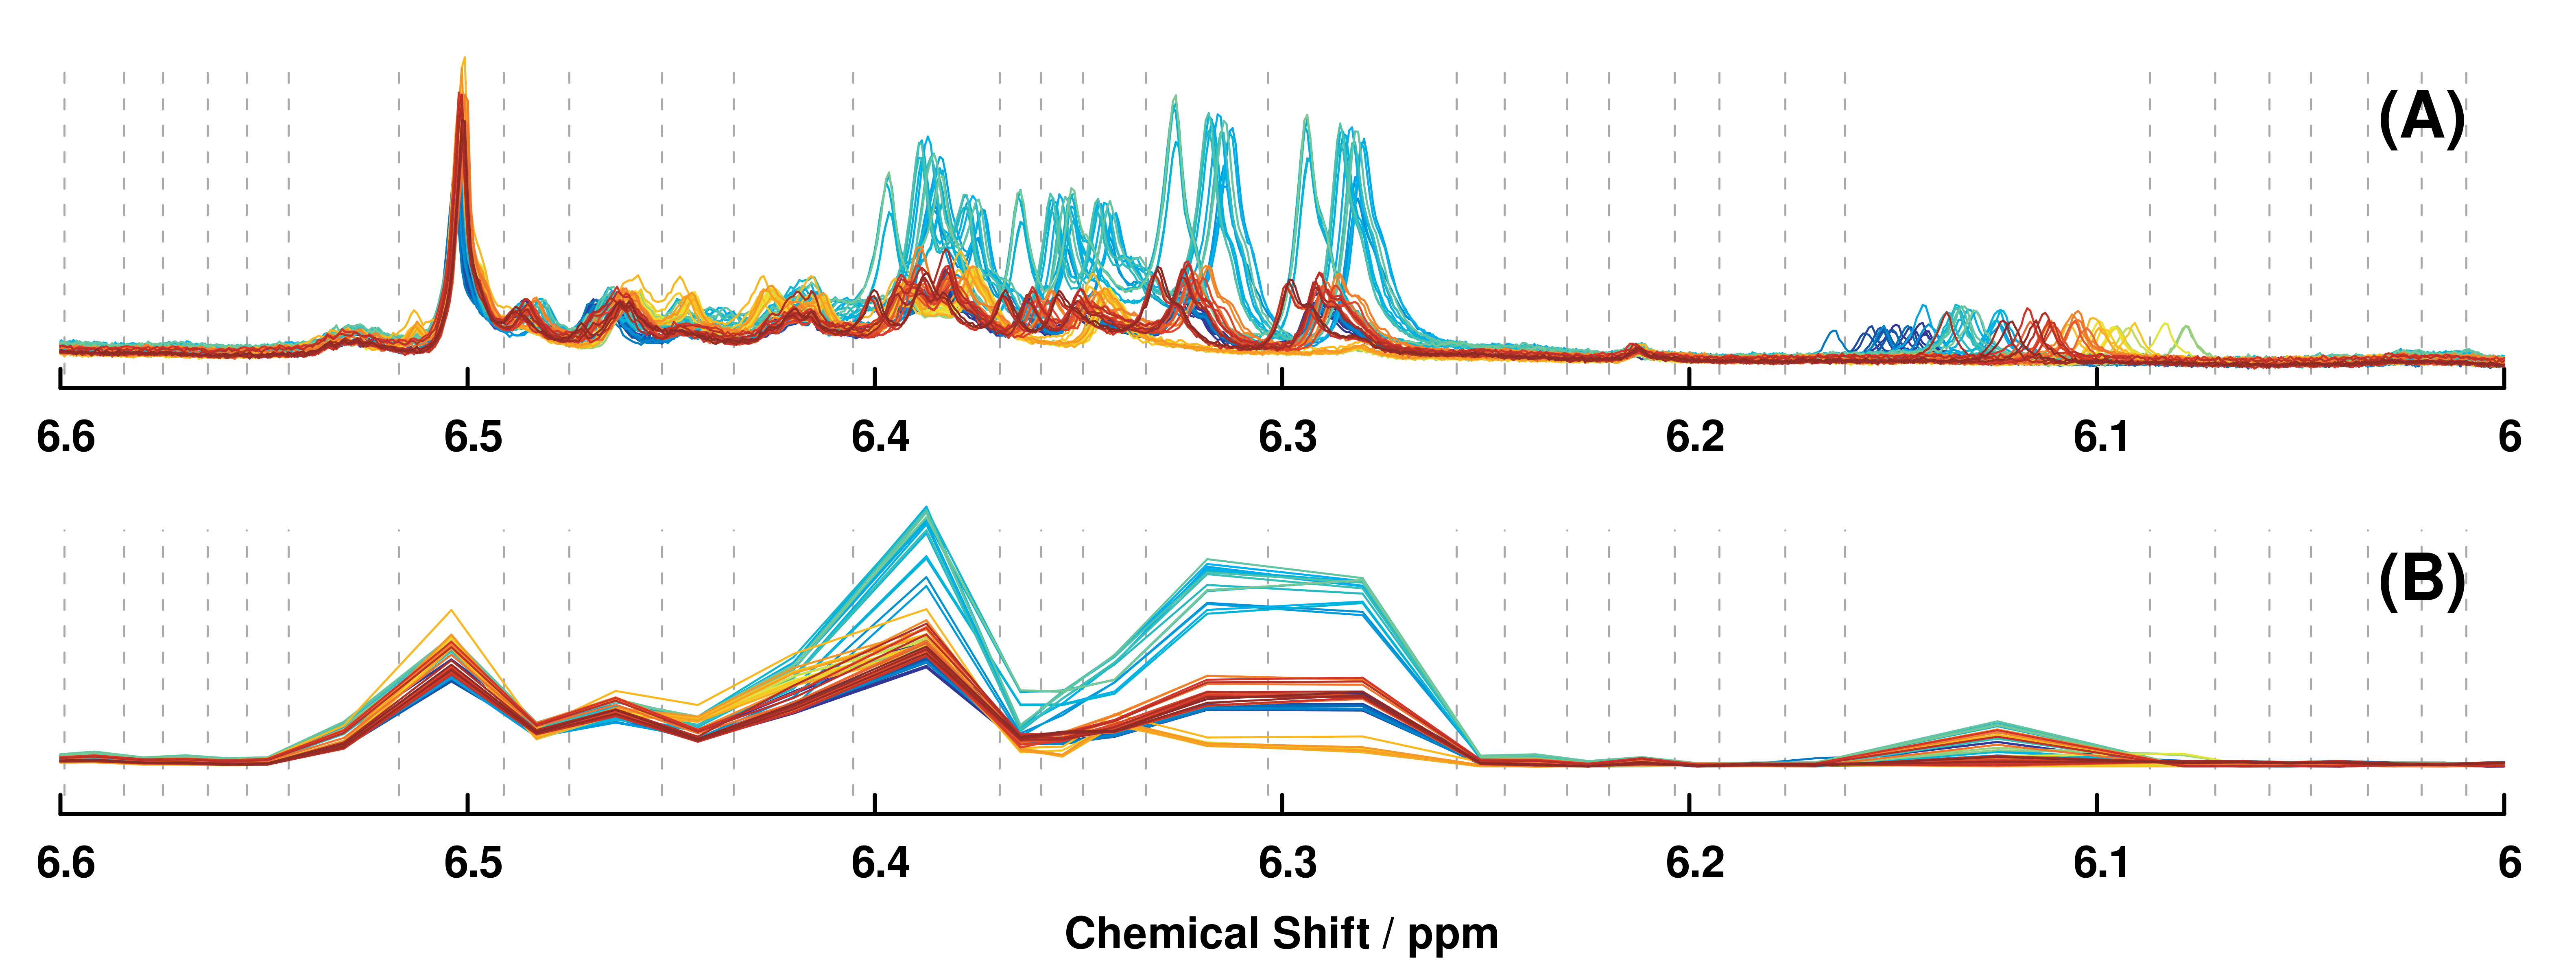
\includegraphics[width=6.5in]{figs/intro/03-bins.png}
\caption
      [Example Binning Result from a 1D \hnmr{} NMR Dataset.]{
  {\bf Example Binning Result from a 1D \hnmr{} NMR Dataset.}
  \\
  Full-resolution ({\bf A}) and adaptively intelligently binned ({\bf B}) 1D
  \hnmr{} NMR spectra from a chemometric study of brewed coffee roasts.
  Spectral color indicates the observation index, and dashed lines indicate bin
  boundaries. Further discussion of binning may be found in Chapters 3 and 6.
}
\end{figure}

\subsection{Modeling and Validation}

\begin{doublespace}
Once a dataset $\mathbf{D}$ has been suitably processed and treated, a model
$f(\mathbf{D})$ may be trained on its contents. Within chemometrics, principal
component analysis (PCA) is undoubtedly the most routinely used modeling
algorithm for describing relationships between multivariate spectral
observations \cite{bro:anmeth2014}, because it provides an unbiased,
simplified picture of the data in a low-dimensional ``scores'' space. The
scores obtained from PCA models of spectral data are useful for determining
statistical distances between experimental groups
\cite{demaesschalck:cils2000,worley:abio2013}, which are effective predictors
of the reliability of any regression models that may be trained on the same
data.
\\\\
Another multivariate algorithm of equal popularity to PCA in chemometrics is
partial least squares (PLS), which is used for solving regression and class
discrimination problems on multivariate data \cite{wold1993}. While PLS
provides a similar low-dimensional scores-space view of spectral observations,
its true power in chemometrics lies in its ability to report ``loadings'',
which are spectral contributions that predict a set of chemical properties.
\\\\
The combination of PCA and PLS as a methodology for studying complex spectral
datasets has proven highly useful in chemometrics, most notably so in the
field of metabolomics \cite{lindon:cmr2000}. However, analysts must take care
when using models produced by these methods, as they have not been determined
using standard (over-determined) least-squares methods and may over-fit a
dataset at the expense of generality, which is required for broad inference
\cite{westerhuis:metab2008a}. Rigorous application of cross-validation methods,
including internal and external cross-validation
\cite{xu:cils2001,eshghi:cils2014}, response permutation testing
\cite{golland:learn2005} and CV-ANOVA \cite{eriksson:jchemo2008}, is required
in order to ensure that trained multivariate models are reliable and
generalizable to later measurements.
\end{doublespace}

\subsection{Inference}

\begin{doublespace}
Once multivariate models have been trained and validated on a given dataset,
they may finally be utilized for the extraction of chemical information from
that dataset. Often, this process of inference revolves around the analysis of
separations between one or more experimental groups in PCA or PLS scores space.
Because scores-space separations are often used as justification for further
costly experimentation, it is important to quantitatively measure these
separations using proper statistical tools \cite{worley:abio2013}.
\end{doublespace}

\section{Summary of Work}

\begin{doublespace}
By and large, this dissertation follows the logical flow of a data analyst
in the field of NMR metabolomics, working from methods in compressive data
acquisition, through a description of multivariate analysis techniques, to
processing, treatment and validation of multivariate modeling results, and
ending with a solution to a bioinformatics data handling problem: the
correlation between high-resolution protein structure and backbone chemical
shifts.
\\\\
\hyperlink{chapter.2}{Chapter 2} begins by introducing a gap-based nonuniform
sampling framework that provides several attractive advantages over traditional
probability density-based nonuniform sampling methods. While most methods of
generating nonuniform sampling schedules rely on randomly sampling from a
specified weighting function that is defined over a Nyquist grid, this new
method of gap sampling builds up schedules based on the value of a `gap
equation' that specifies the spacing between sampled Nyquist grid points. The
gap sampling framework is first defined, and comparisons in performance are
made between specific forms of gap sampling and the stochastic Poisson-gap
sampling method from Hyberts and Wagner \cite{hyberts:jacs2010}.
\\\\
A comprehensive description of the required data handling tasks -- steps
{\bf (1-9)} in Figure 1.1 -- in metabolic fingerprinting and untargeted
metabolic profiling studies is provided within
\hyperlink{chapter.3}{Chapter 3}. Additional practical guidelines on the
relationship between class separations in PCA scores space and reliability
of OPLS-DA models on the same data are also presented. Examples of applied
multivariate analysis in metabolomics are given in
\hyperlink{chapter.4}{Chapter 4}.
\\\\
\hyperlink{chapter.5}{Chapter 5} introduces the MVAPACK toolbox for
chemometrics as a complete solution to the data handling problem in NMR-
and MS-based metabolomics studies. Beginning with a set of raw free induction
decays from an NMR spectrometer, analysts may now rapidly and easily generate
validated multivariate models using rigorously tested and peer-reviewed
routines in MVAPACK. As a result, both the turnaround time between data
collection and interpretation and the likelihood of analyst error are
dramatically reduced when using MVAPACK. The architecture and design rationale
of the MVAPACK toolbox are discussed in this chapter.
\\\\
\hyperlink{chapter.6}{Chapter 6} and \hyperlink{chapter.7}{Chapter 7} focus on
a novel method of data processing (Phase-scatter Correction) and describe its
application on datasets acquired from both metabolomics and high-throughput
protein-ligand affinity screens. \hyperlink{chapter.8}{Chapter 8} introduces
a novel method of data treatment (Generalized Adaptive Intelligent Binning)
that enables the direct use of multidimensional data tensors in PCA and PLS
modeling. Both phase-scatter correction and GAI-binning were developed within
the MVAPACK toolbox, which was specifically for efficient management of NMR
spectral data. \hyperlink{chapter.9}{Chapter 9} describes a small set of
portable utilities that generate statistically sound dendrograms of
scores-space class relationships using both bootstrap-based and parametric
methods.
\\\\
\hyperlink{chapter.10}{Chapter 10} outlines the generation of a set of
bioinformatic tools to analyze the relationship between the geometry of
interacting pairs of carbonyls in protein backbones and their \cnmr{} chemical
shift values \cite{worley:pone2012}. These tools, combined with quantum
chemical computations, provide strong evidence for the nonexistence of
\npistar{} interactions between these carbonyl groups in native protein
structures.
\\\\
Finally, \hyperlink{chapter.11}{Chapter 11} summarizes the solutions provided
herein to a set of chemometrics and bioinformatics data handling problems and
discusses challenges and avenues of effort that will be required to solve
future problems of the same kind.
\end{doublespace}

\bibliographystyle{abbrv}
\bibliography{bworley}



\chapter{Multidimensional Nonuniform Gap Sampling}

\begin{quote}
{\it
  Anyone who considers arithmetical methods of producing random digits is,
  of course, in a state of sin.}
\\\\
 -- John von Neumann
\end{quote}

\section{Introduction}

\begin{doublespace}
The use of nonuniform sampling in multidimensional NMR is rapidly becoming
standard practice in most biomolecular solution-state experiments, thanks in
large part to recent developments in fast reconstruction algorithms, novel
sampling schemes, and the continually declining cost of computing power
\cite{mobli:pnmrs2014}. The potential benefits of collecting a subset of the
full Nyquist grid -- including increased sensitivity and signal-to-noise,
improved resolution, and reduced experiment time -- have received significant
attention \cite{
  rovnyak:jmr2004, rovnyak:jbnmr2004, kazimierczuk:angew2011,
  hyberts:jbnmr2013, palmer:jbnmr2014} in recent years as a consequence.
\\\\
One intriguing result of recent investigations into the parameters of NUS
experiments is the use of random deviates for generating sampling schedules
\cite{hoch:jmr2008}. In fully random sampling schemes, a subset of Nyquist
grid points is drawn from a probability density function that varies over the
grid, producing a sampling schedule with a desired distribution of points.
Common fully random sampling schemes utilize uniform, exponential, Gaussian
and envelope-matched probability densities
\cite{palmer:jbnmr2014,schuyler:jbnmr2011}. While randomization is a simple
means of reducing the artifacts due to aliasing of nonuniformly spaced samples,
it turns the already complex task of schedule generation into that of selecting
a schedule from an ensemble of possibilities, each of which performs
differently in practice \cite{hyberts:jacs2010,mobli:jmr2015}. Several ad hoc
metrics have been proposed to assess the relative performance sampling
schedules, but no universally accepted metric exists to guide the selection
of a stochastic schedule from its ensemble \cite{mobli:jmr2015,aoto:jmr2014}.
Without a priori knowledge of the frequency and decay rate distributions of
the signals to be measured, it is difficult to reliably quantify sampling
schedule performance \cite{mobli:pnmrs2014,schuyler:jbnmr2011}. As a result,
numerous recent attempts have been made to reduce or remove pseudorandom
seed-dependent variability from nonuniform sampling algorithms
\cite{kazimierczuk:jmr2007,hyberts:jacs2010,eddy:jmr2012,mobli:jmr2015}.
Such efforts are an important step towards increasing the practical utility
of nonuniform sampling in everyday spectroscopic experiments.
\\\\
Through an empirical analysis of Forward Maximum Entropy (FM) reconstructions
of randomly sampled data, Hyberts et al. proposed the use of constrained
Poisson random deviates to define the \emph{gaps} between sampled points
in a Nyquist grid \cite{hyberts:jacs2010}. The FM reconstruction residuals
of these so-named Poisson-gap schedules exhibited a markedly lower dependence
on seed value than unconstrained random sampling methods. While Poisson-gap
sampling yields high-quality reconstructions of NUS spectral data, its average
behavior is not well-understood, its implementation for multidimensional
Nyquist grids is unclear
\cite{hyberts:tcc2012,hyberts:jbnmr2012,hyberts:jmr2014},
and its relationship -- if any -- to fully random sampling is unknown.
To meet this need, this work describes in detail the deterministic generation
of sinusoidally weighted multidimensional gap schedules that model the average
behavior of stochastic Poisson-gap (PG) sampling. An expectation sampling
probability distribution is also derived that reflects the average weighting
obtained using one-dimensional Poisson-gap sampling schedules.
\\\\
Among the myriad of different sampling schemes proposed for NUS data
collection \cite{maciejewski:tcc2012}, burst-mode sampling similarly concerns
itself with gaps between sampled grid points. Unlike Poisson-gap sampling,
which aims to minimize the \emph{length} of gaps, burst-mode sampling aims
to minimize the \emph{number} of gaps while keeping the effective dwell time
low \cite{maciejewski:jmr2009}. We leverage the complementarity of burst-mode
and Poisson-gap sampling in our deterministic gap sampling algorithm to
describe a novel sampling scheme that simultaneously seeks to bias sample
collection to early times, minimize the number of long gaps between densely
sampled regions, and minimize the largest gap length in the schedule. The
resulting method, called sine-burst (SB) sampling, exhibits the high
performance of Poisson-gap sampling while retaining the bijective mapping
between inputs and outputs offered by deterministic methods.
\end{doublespace}

\section{Theory}

\subsection{Poisson-gap Sequences}

\begin{doublespace}
Gap schedules on a one-dimensional Nyquist grid are effectively finite integer
sequences, computed from the following recurrence relation:
\begin{equation}
x_{i+1} = x_i + \lfloor g(x_i) \rfloor + 1
\end{equation}
where $x_i$ is the grid index of the $i$-th term in the sequence and $g(x_i)$
is the ``gap equation'' that defines the distance between terms. The first term
in the sequence, $x_1$, is set to 1 and subsequent terms are computed until
their value exceeds $N$, the size of the grid. The gap equation $g(x)$ may be
any non-negative function, and may be loosely interpreted as inversely related
to the local sampling density at the grid index $x_i$. Thus, when the gap
equation equals zero for all grid indices, gap sampling will yield a uniformly
sampled grid.
\\\\
Poisson-gap sequences treat the gap equation as a Poisson random deviate
having a rate parameter that varies as either a quarter- or half-sinusoid
over the grid indices:
\begin{equation}
g_{PG}(x_i) \sim \mathrm{Pois} \left\{
 \Lambda \sin \left(
  \frac{\pi}{2} \theta_i
 \right)
\right\}
\end{equation}
where $\Lambda$ is a scaling factor that determines the global sampling
density and $\theta_i$ is the fractional grid index that varies from 0 to 1
over the grid extents:
\begin{equation}
\theta_i = \frac{x_i}{N}
\end{equation}

In all following descriptions of Poisson-gap methods, we shall restrict our
attention to rate parameters which vary as quarter-sinusoids, where the
fractional grid index is multiplied by a factor of one-half $\pi$. This choice
of sinusoidal weight produces schedules that are heavily biased to earlier
grid points. Using a factor of $\pi$ produces half-sinusoidal rate parameters
and schedules that are more densely sampled at both early and late grid points.
\\\\
Because the expected value of a Poisson distribution is equal to its rate
parameter, one may trivially construct a deterministic sinusoidally weighted
gap sampler (sine-gap; SG) by setting the gap equation equal to the scaled
quarter-sinusoid from equation 2.2, as follows:
\begin{equation}
g_{SG} = \Lambda \sin \left( \frac{\pi}{2} \theta_i \right)
\end{equation}

By construction, gap sampling schedules computed according to $g_{SG}$ will
describe the average behavior of $g_{PG}$. This is readily verified in one
dimension by generating a sufficiently large set of stochastic Poisson-gap
schedules and comparing the mean value of each sequence term to that of a
sine-gap schedule (\figref{2.1}{Figure 2.1}). Sine-gap schedules
lie centrally within the Poisson-gap ensemble, while other schedules
unrelated to Poisson-gap deviate substantially from the confidence
region of the ensemble.
\end{doublespace}

\begin{figure}[ht!]
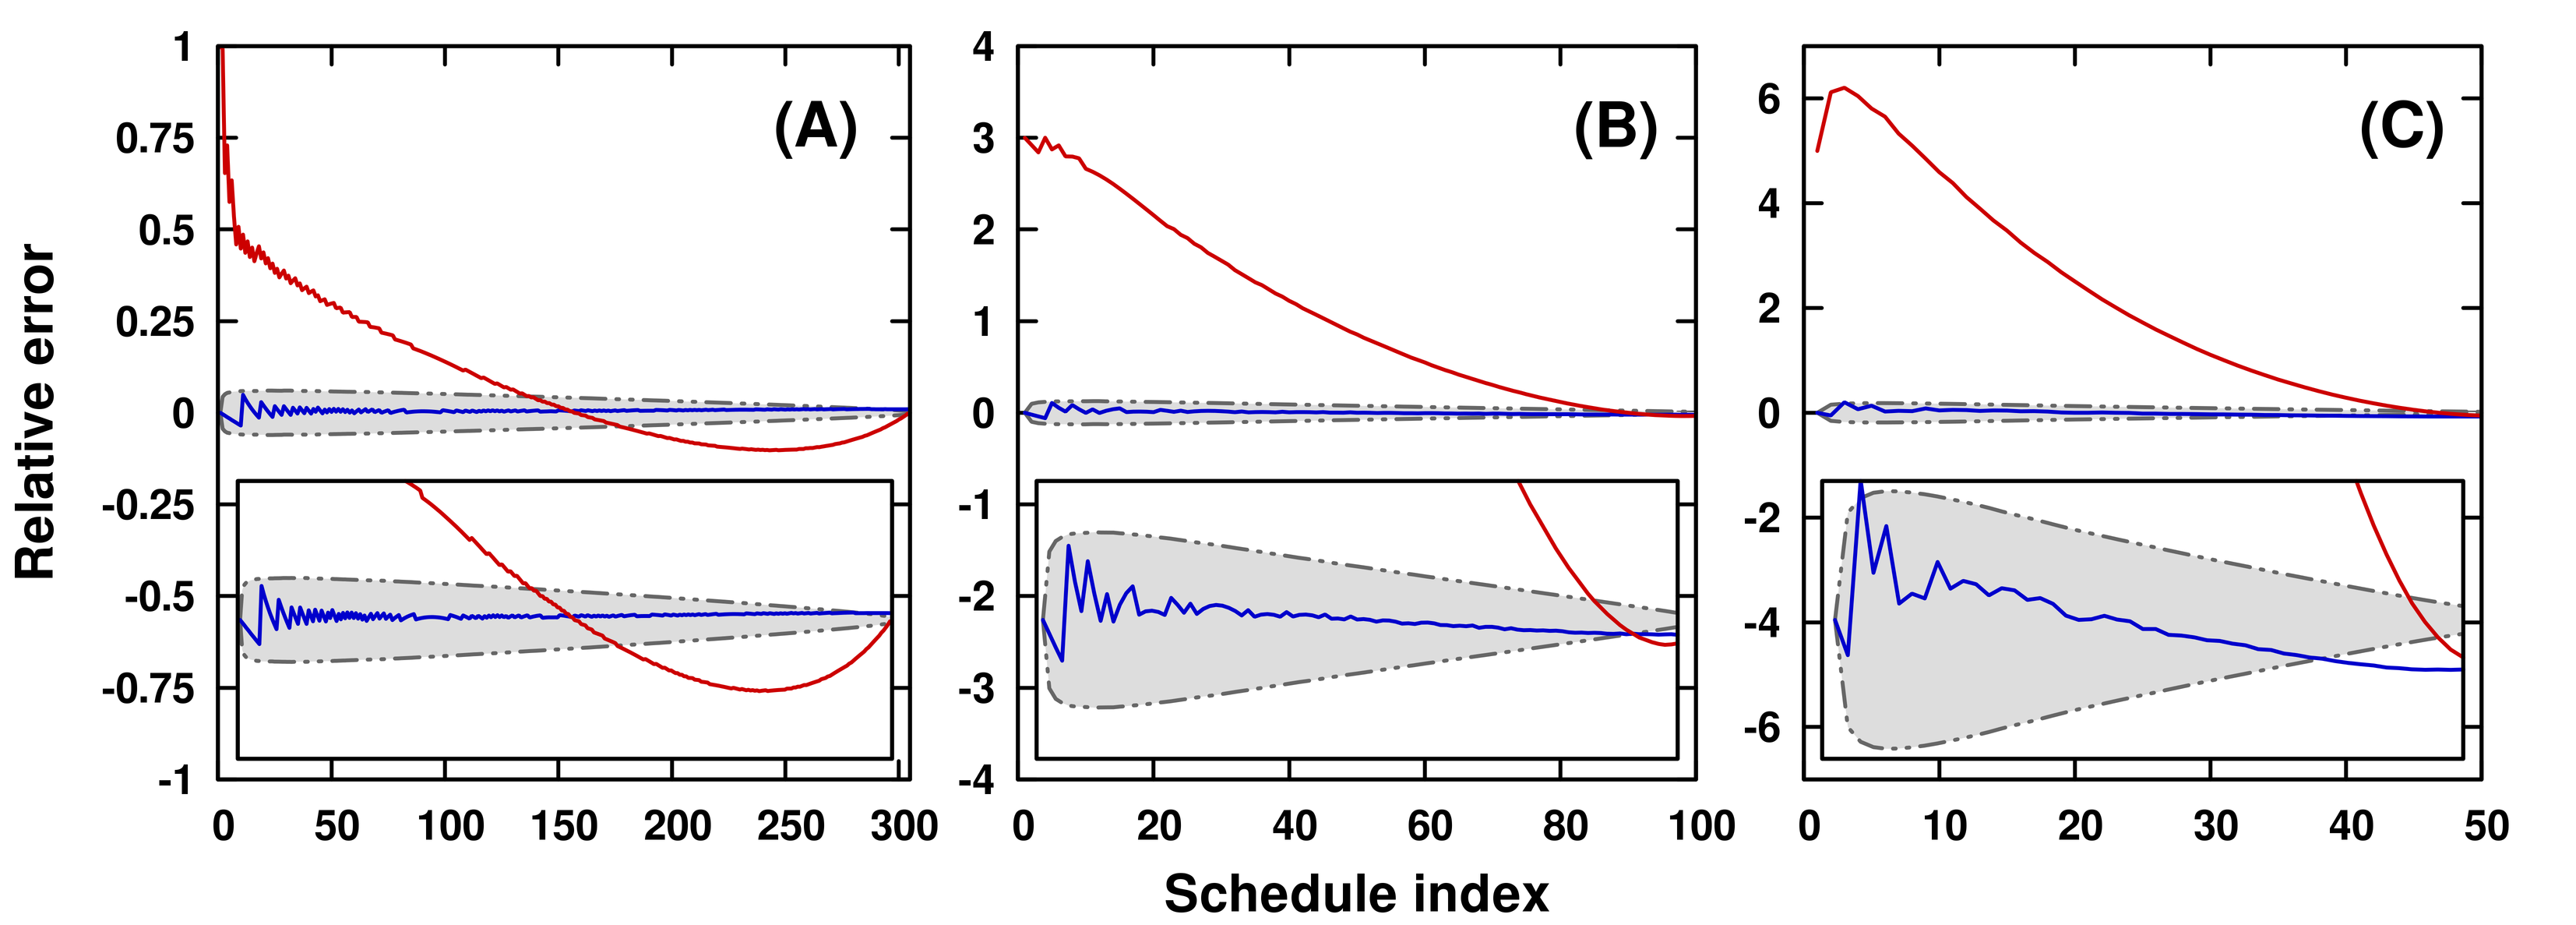
\includegraphics[width=6in]{figs/dgs/01-avepg.png}
\caption
      [Agreement between Poisson-gap and sine-gap Sequences.]{
  {\bf Agreement between Poisson-gap and sine-gap Sequences.}
  \\
  Relative errors between sine-gap (blue lines) and deterministic exponential
  (red lines) schedules with respect to the average Poisson-gap schedule at
  ({\bf A}) 30\% density, ({\bf B}) 10\% density and ({\bf C}) 5\% density.
  Confidence intervals indicating plus or minus one standard deviation of the
  Poisson-gap ensemble are shown as grey shaded regions. The vertical axes of
  all inset plots range from $-0.2$ to $0.2$. Because the sine-gap schedules
  describe the average behavior of the Poisson-gap equation, they lie
  centrally within the Poisson-gap ensemble, while any other schedule
  unrelated to Poisson-gap (e.g. exponential) does not.
}
\label{figure.2.1}
\end{figure}

\subsection{Multidimensional Gap Sampling}

\begin{doublespace}
Gap schedules on a Nyquist grid having at least two dimensions are generated
by placing multiple one-dimensional sub-schedules onto the grid, each with a
different direction and offset from the grid origin. In practice, this process
is accomplished recursively, with planes built up from vectors, cubes built up
from planes, and so forth. Initially, recursion begins on the entire grid. At
each level of recursion, sub-grids are constructed by ``masking off'' each
available grid direction in turn and constructing the remaining unmasked
directions. For example, a three-dimensional $xyz$ cube will be constructed
from repeated sequences of $yz$, $xz$ and $xy$ planes, and each $xy$ plane
will be constructed from repeated sequences of $y$ and $x$ vectors. Once a
round of sub-grid construction has been performed along each direction, the
sub-grid offset is incremented and the process is repeated until no more
sub-grids remain at the current level of recursion. The following executable
pseudocode provides a more precise definition of the recursive gap sampling
algorithm:
\end{doublespace}

\begin{algorithm}[H]
\caption{Multidimensional Gap Sampling Algorithm}
\label{algorithm.2.1}
\begin{python}
def build(N, origin, mask):
  D = len(N)
  if sum(mask) == 1:
    direction = mask.index(1)
    dirstring = ['x', 'y', 'z'][direction]
    print('sequence along ' + dirstring + ' at origin ' + origin)
    return

  suborigin = [0,] * D
  submask = [0,] * D
  done = False
  offset = 0

  while not done:
    done = True
    for direction in range(D):
      if mask[direction] != 1 or offset >= N[direction]:
        continue

      done = False
      for d in range(D):
        if d != direction and mask[d] == 1:
          submask[d] = 1
        else:
          submask[d] = 0

        if d == direction:
          suborigin[d] = offset
        else:
          suborigin[d] = origin[d]

      build(N, suborigin, submask)
    offset = offset + 1

build([8, 4, 4], [0, 0, 0], [1, 1, 1])
\end{python}
\end{algorithm}

\begin{doublespace}
Creation of multidimensional gap schedules requires a slight modification to
the fractional index, which now assumes the following form:
\begin{equation}
\theta_i = \frac{x_i + \sum_{d=1}^D O_d}{\sum_{d=1}^D N_d}
\end{equation}
where $O_d$ and $N_d$ are the origin and grid size along direction $d$,
respectively. The above equation is referred to as ``ADD'' mode in the context
of stochastic Poisson-gap sampling, and effectively results in multidimensional
schedules that exhibit triangular forms \cite{hyberts:jmr2014}. It is worthy of
mention that, in the one-dimensional case, equation 2.5 reduces to equation
2.3.
\\\\
Finally, whether the Nyquist grid is one- or many-dimensional, a value of the
global scaling factor $\Lambda$ must be determined that yields the desired
number of sampled grid points. Our gap sampling implementation, like the
existing Poisson-gap method, iteratively rebuilds new schedules until
$\Lambda$ has been suitably optimized.
\end{doublespace}

\subsection{Burst Augmentation}

\begin{doublespace}
Recent statistical descriptions of the discrete Fourier transform have shown
that the bandwidth of a nonuniformly sampled signal is related to the greatest
common factor of the gaps between sampled grid points
\cite{bretthorst:cmr2008}. One proposed method of increasing bandwidth and
reducing artifacts in NUS data is to sample in multiple short bursts having
zero gap length \cite{maciejewski:jmr2009}. Using gap sampling, this may be
accomplished by modulating the gap equation between zero and its maximum value
several times over the Nyquist grid, like so:
\begin{equation}
g_{SB}(x_i; d) = \Lambda
 \sin \left( \frac{\pi}{2} \theta_i \right)
 \sin^2 \left( \frac{\pi}{4} N_d \theta_i \right)
\end{equation}

The sine-burst gap equation $g_{SB}$ combines the sinusoidal forward-biasing
and minimized gap lengths of Poisson-gap sampling with the minimized effective
dwell time of burst-mode sampling, and does not require the use of random
deviates to achieve reasonable artifact suppression.
\end{doublespace}

\begin{figure}[ht!]
\begin{center}
  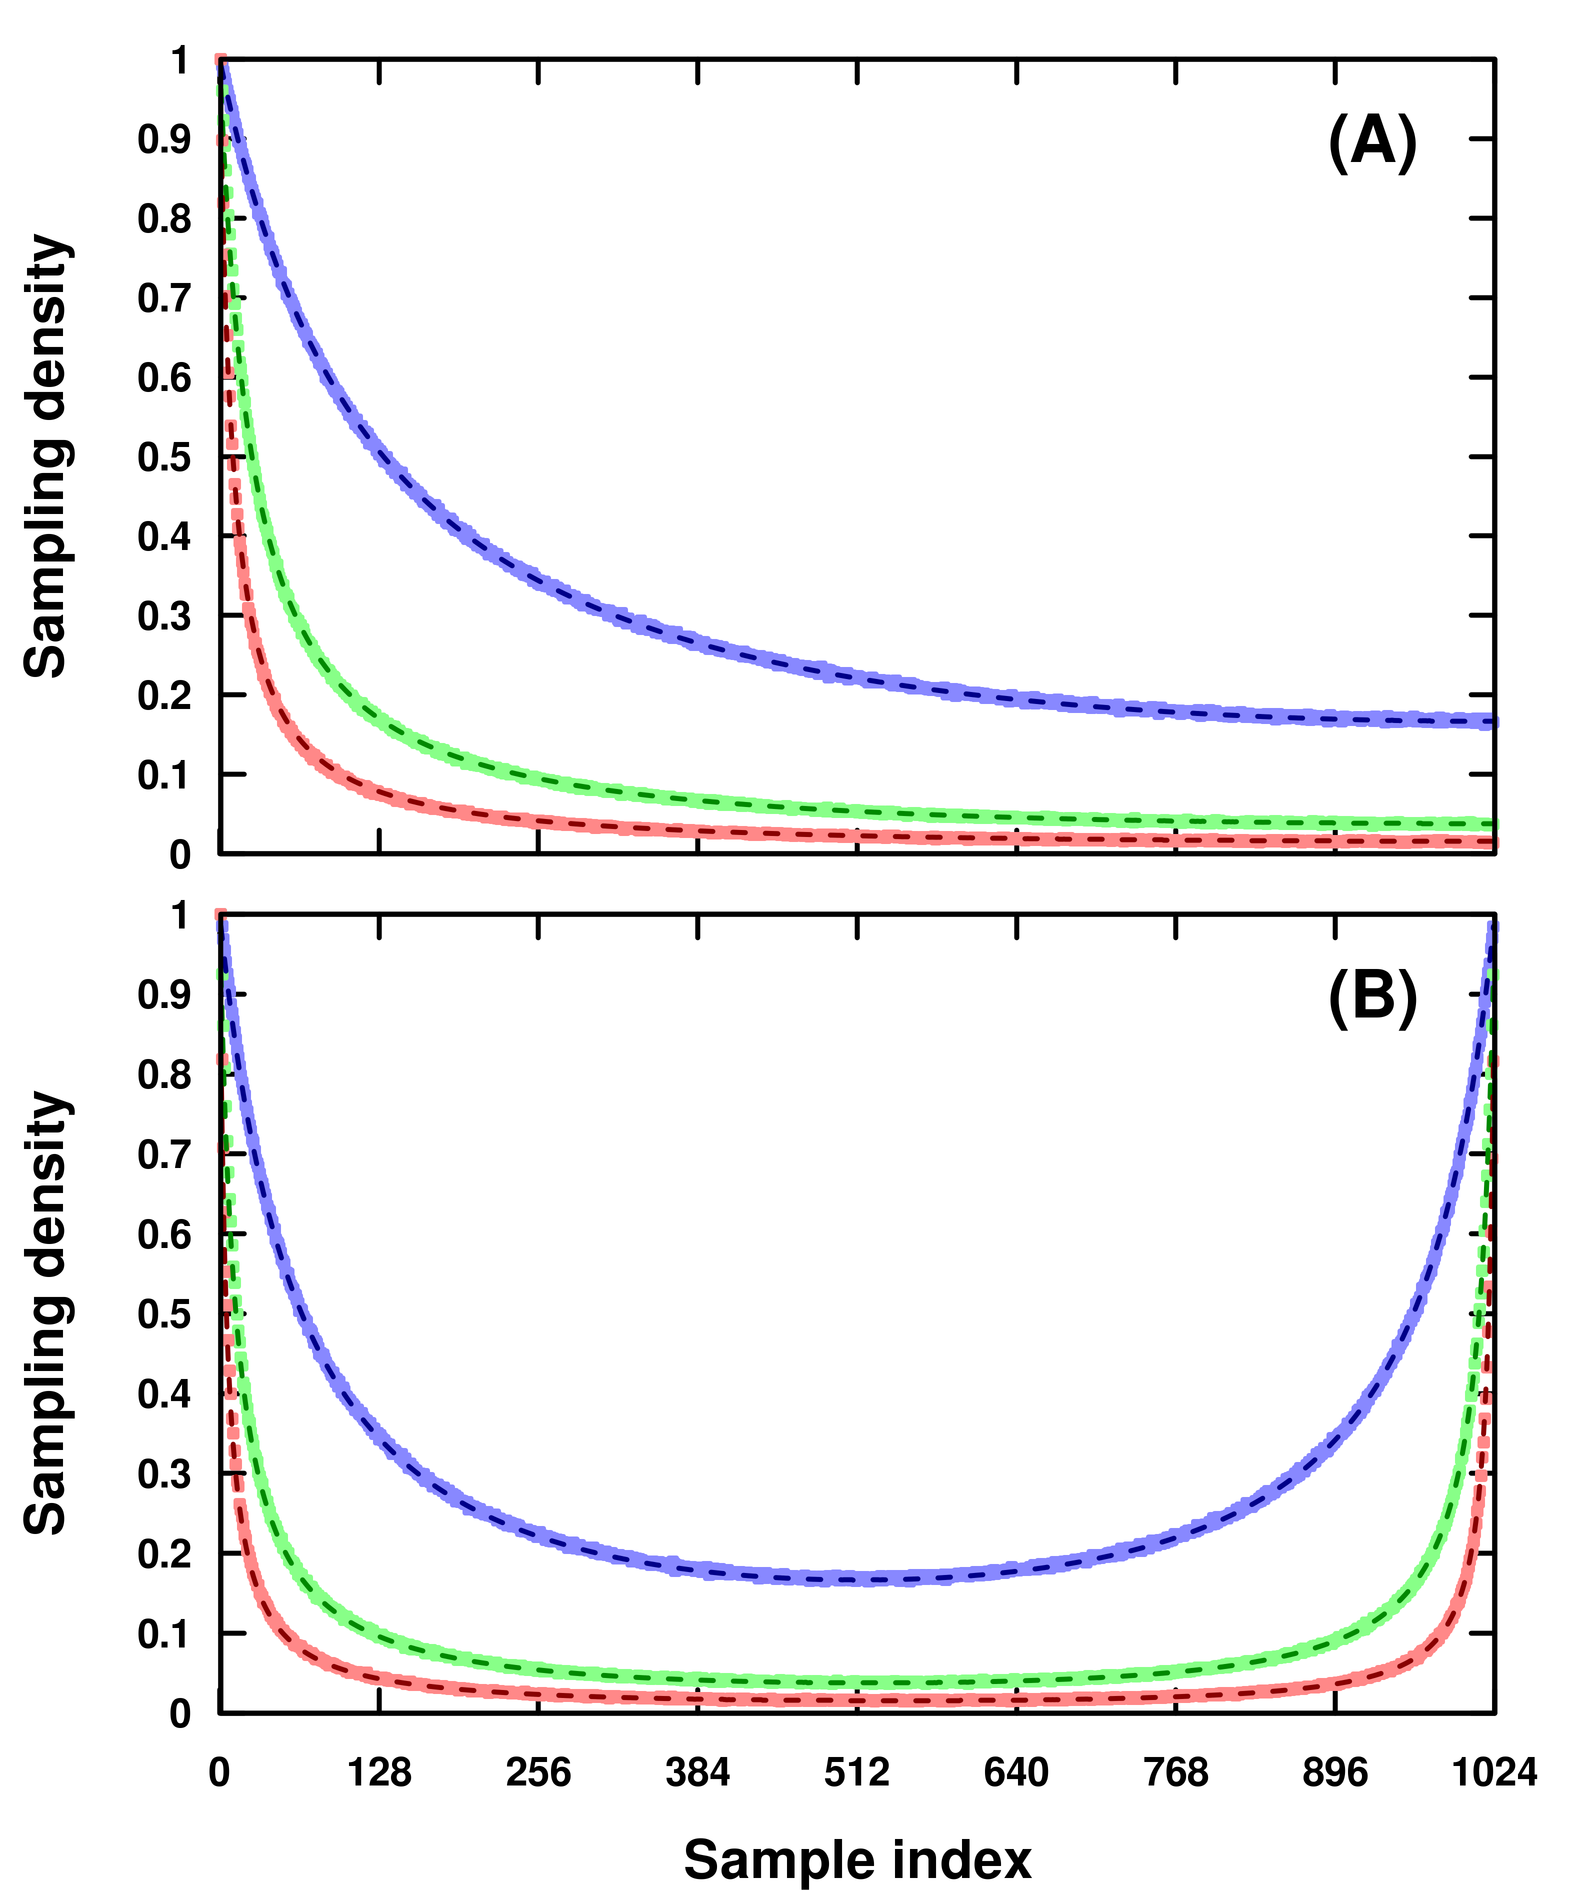
\includegraphics[width=4.5in]{figs/dgs/02-expect-1d.png}
\end{center}
\caption
      [Poisson-gap 1D Expectation Sampling Distributions.]{
  {\bf Poisson-gap 1D Expectation Sampling Distributions.}
  \\
  Expectation sampling distributions computed by averaging 50,000
  one-dimensional Poisson-gap schedules of varying densities, with
  quarter-sinusoidal ({\bf A}) and half-sinusoidal ({\bf B}) weightings.
  The lighter blue, green and red points were computed from schedules having
  30\%, 10\% and 5\% sampling density, respectively. The dashed lines overlaid
  on each set of points correspond to the analytic sampling distribution
  (equation 2.11) derived from $g_{PG}$. Values of $\Lambda$ were 5.0, 25.4
  and 62.9 for 30\%, 10\% and 5\% sampling density, respectively.
}
\label{figure.2.2}
\end{figure}

\subsection{Expectation Sampling Distributions}

\begin{doublespace}
One disadvantage of stochastic gap equations is that they provide no direct
measure of how likely each Nyquist grid point is to be sampled. While one may
speculate on the approximate weighting obtained by a given gap equation,
quantitation of the expectation of the sampling distribution requires the
construction and averaging of a large number of sampling schedules
(cf. \figref{2.2}{Figures 2.2}, \figref{2.3}{2.3} and \figref{2.4}{2.4}).
Fortunately, the expectation sampling distribution of a given gap equation
may be analytically obtained by computing the probability of sampling each
point on the grid using a recursive formula. We define an expectation
sampling distribution $p(i)$ that varies over a one-dimensional Nyquist
grid of $N$ points as follows:
\begin{equation}
p(i) = \sum_{k=1}^{i-1} p(i \mid i-k) p(i-k)
\end{equation}
where $p(i \mid i-k)$ is the probability of grid point $i$ being emitted from
grid point $i-k$, which requires a gap size of $k-1$:
\begin{equation}
p(i \mid i-k) = \mathrm{Pr}\left\{
 \lfloor g(i-k) \rfloor = k - 1
\right\}
\end{equation}

In other words, the probability of sampling any given grid point is the
weighted sum of the probabilities of arriving at that point from all prior
points. In the case of Poisson-gap sampling, the gap equation is a Poisson
random deviate:
\begin{equation}
\mathrm{Pr}\left\{ \lfloor g(x_i) \rfloor = k - 1 \right\} =
 \frac{\lambda(x_i)^{k-1}}{(k-1)!} e^{-\lambda(x_i)}
\end{equation}
where the rate parameter $\lambda(x_i)$ varies sinusoidally over the Nyquist
grid:
\begin{equation}
\lambda(m) = \Lambda \sin \left( \frac{\pi m}{2 N} \right)
\end{equation}

By combining the above four equations, we arrive at the sampling distribution
of a one-dimensional Poisson-gap sequence:
\begin{equation}
p(i) = \sum_{k=1}^{i-1} \frac{\Lambda^{k-1}}{(k-1)!}
 \sin^{k-1} \left( \frac{\pi [i-k]}{2 N} \right)
 \exp\left\{
  -\Lambda \sin \left( \frac{\pi [i-k]}{2 N} \right)
 \right\}
p(i-k)
\end{equation}

As in the case of gap sampling, the sampling distribution produced by equation
2.11 is parameterized only by the scaling factor $\Lambda$, where larger values
yield more forward-biased schedules (\figref{2.2}{Figure 2.2}). We refer
to this equation as the ``expectation'' Poisson-gap sampling distribution
because it describes the expected value of the probability of sampling any
Nyquist grid point, and is not itself useful for generating schedules that
obey $g_{PG}$.
\end{doublespace}

\begin{figure}[ht!]
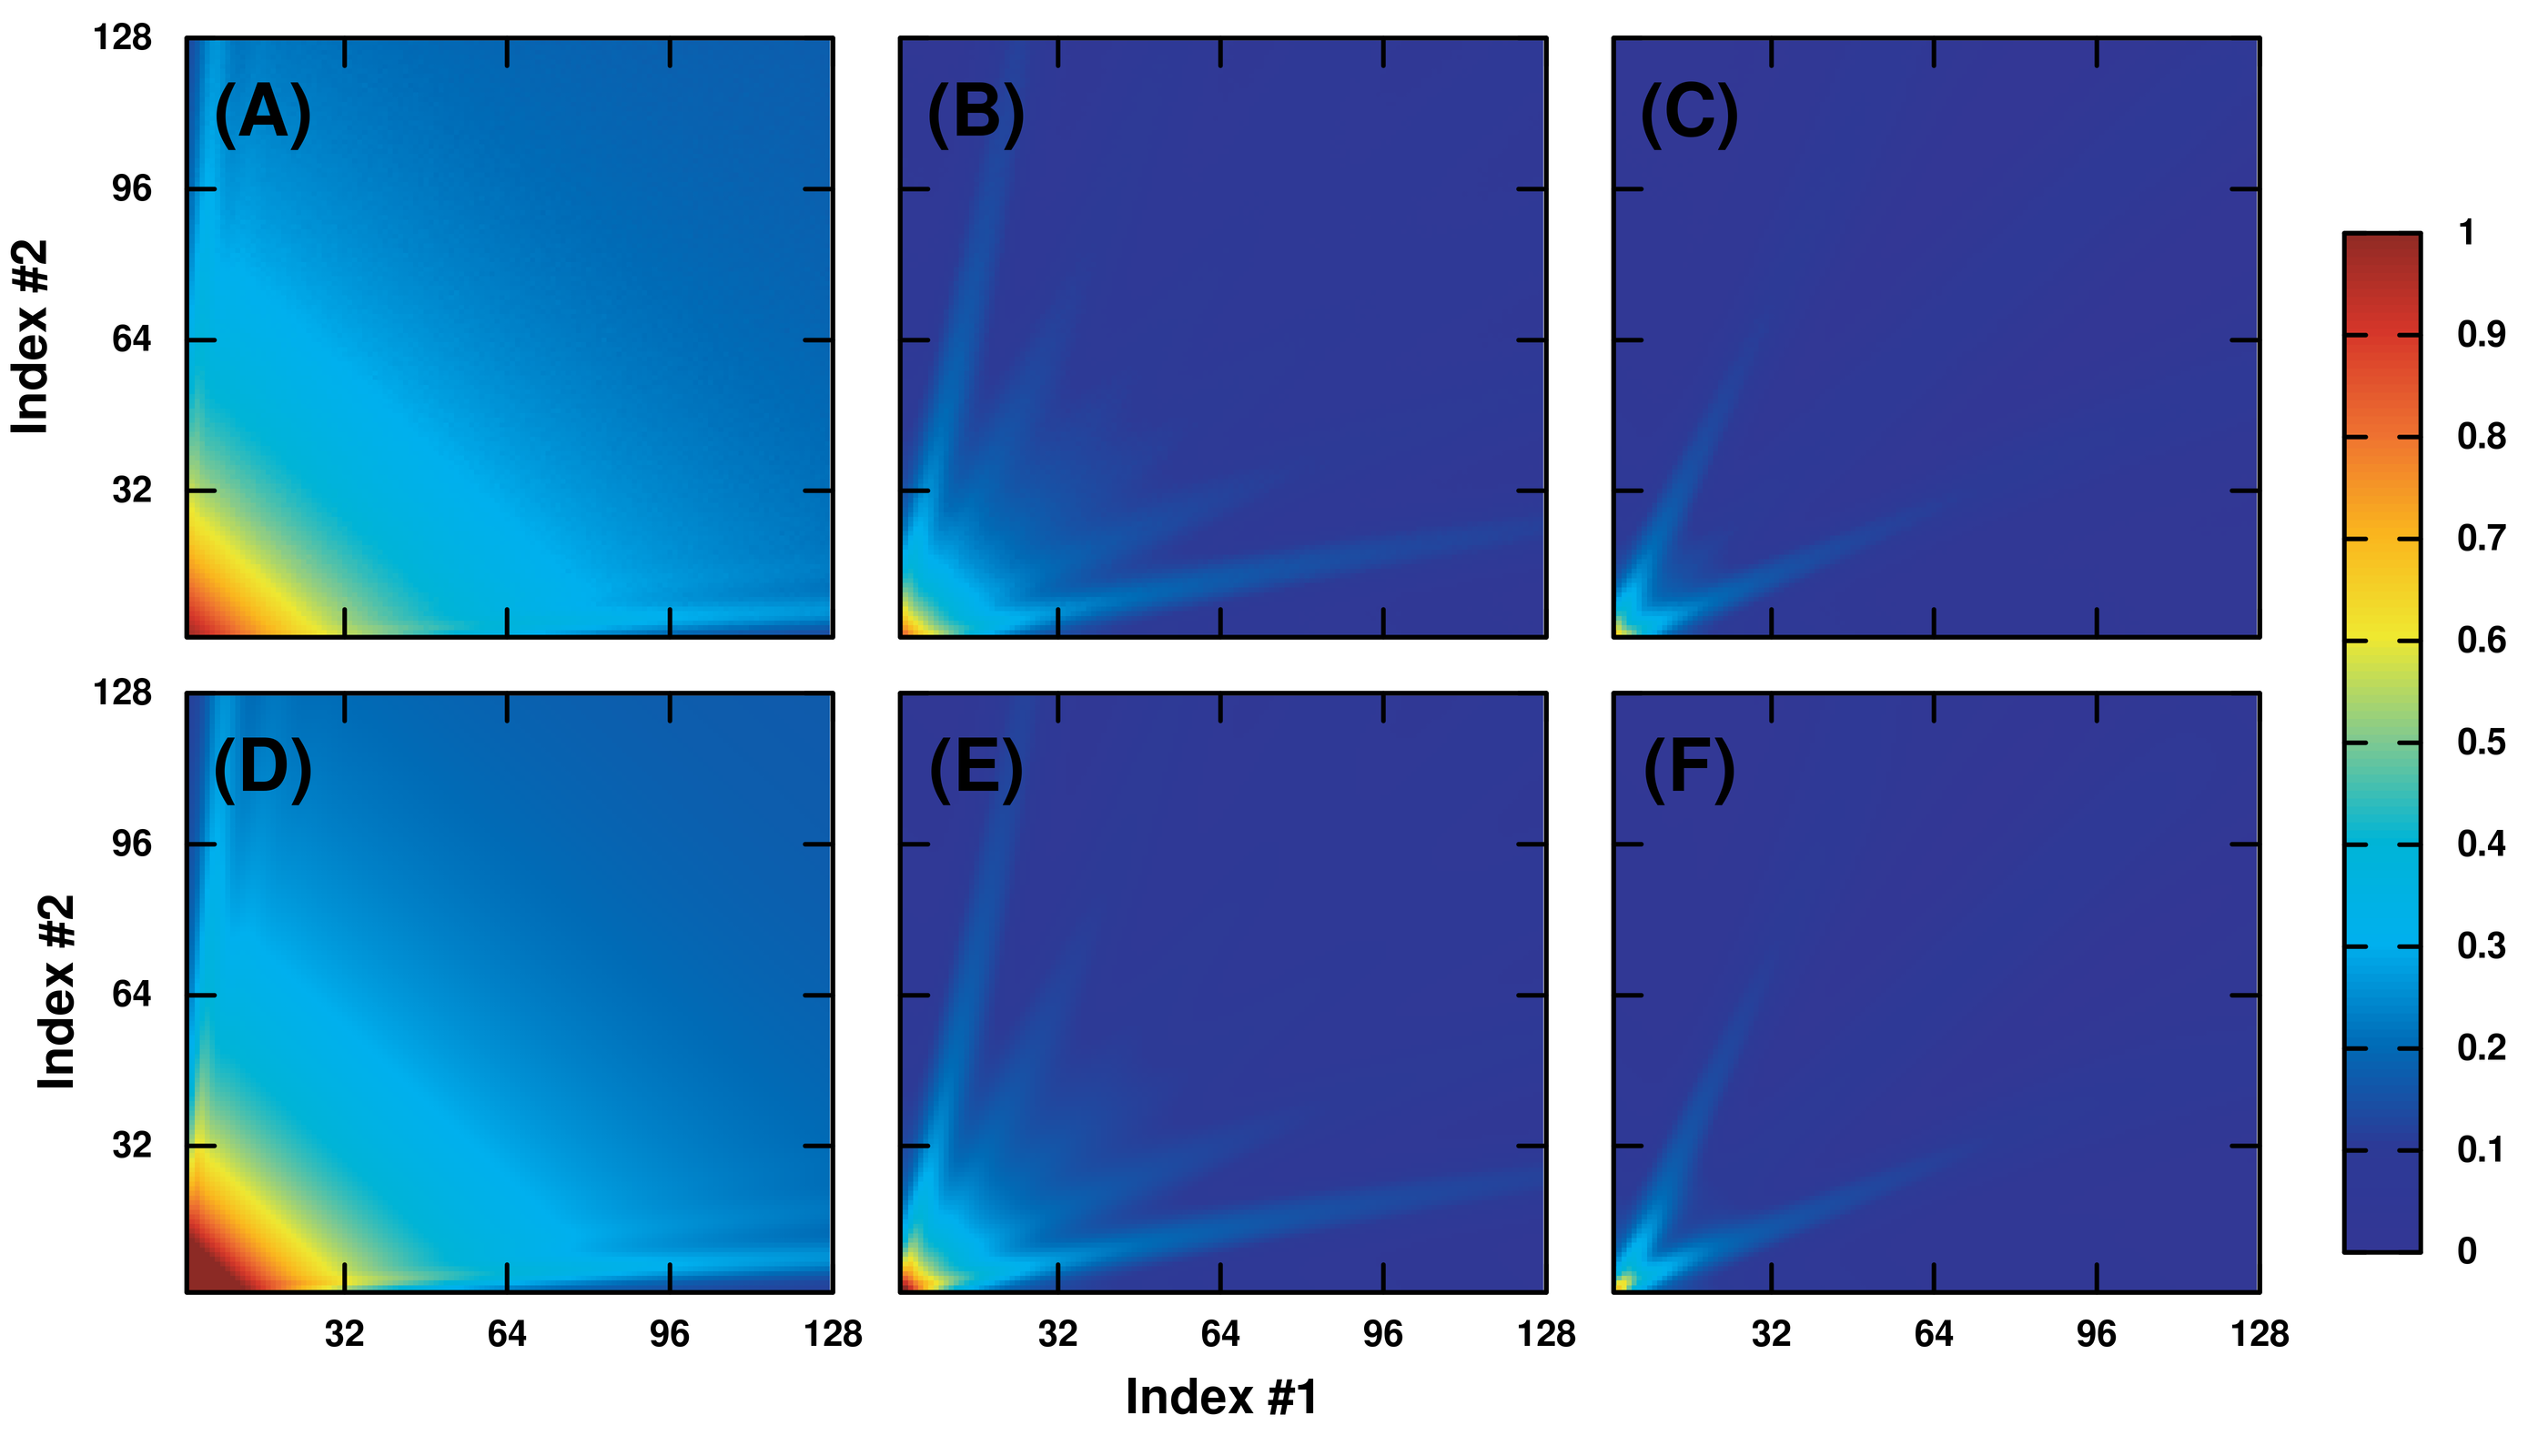
\includegraphics[width=6in]{figs/dgs/03-expect-2d.png}
\caption
      [Poisson-gap 2D Expectation Sampling Distributions.]{
  {\bf Poisson-gap 2D Expectation Sampling Distributions.}
  \\
  Expectation sampling distributions of two-dimensional Poisson-gap schedules
  computed in strict accordance to Algorithm 2.1. Top panels were produced by
  averaging 50,000 two-dimensional schedules, and bottom panels were computed
  using equation 2.12 with appropriate substitutions of the Poisson
  probability mass function. Sampling densities of 30\%, 10\% and 5\% are
  shown in panels ({\bf A}, {\bf D}), ({\bf B}, {\bf E}) and
  ({\bf C}, {\bf F}), respectively.
}
\label{figure.2.3}
\end{figure}

\begin{figure}[ht!]
\includegraphics[width=6in]{figs/dgs/04-expect-hyb.png}
\caption
      [Poisson-gap 2D Expectation Sampling Distributions.]{
  {\bf Poisson-gap 2D Expectation Sampling Distributions.}
  \\
  Expectation sampling distributions computed by averaging 50,000
  two-dimensional Poisson-gap schedules generated using code provided by
  Hyberts and Wagner. Sampling densities of 30\%, 10\% and 5\% are
  shown in panels ({\bf A}), ({\bf B}) and ({\bf C}), respectively.
}
\label{figure.2.4}
\end{figure}

\subsection{Multidimensional Expectation Sampling Distributions}

\begin{doublespace}
Extension of equation 2.11 to compute the expectation sampling distributions
of stochastic gap equations in two or more dimensions follows from the fact
that sampling along each direction is essentially independent of other
directions within the presented gap sampling framework. As a consequence,
the probability of sampling any multidimensional grid point is therefore the
sum of sampling that point along each grid direction. For a two-dimensional
grid $(i_1,i_2)$, the expectation sampling distribution is the sum of the
probability matrices $p_1(i_1,i_2)$ and $p_2(i_1,i_2)$:
\begin{align}
p_1(i_1,i_2) =& \sum_{k=1}^{i_1-1} p(i_1,i_2 \mid i_1-k,i_2) p_1(i_1-k,i_2)
 \nonumber \\
p_2(i_1,i_2) =& \sum_{k=1}^{i_2-1} p(i_1,i_2 \mid i_1,i_2-k) p_2(i_1,i_2-k)
 \nonumber \\
p(i_1,i_2) =&\: p_1(i_1,i_2) + p_2(i_1,i_2)
\end{align}

\figref{2.3}{Figure 2.3} illustrates the expectation Poisson-gap sampling
distribution on two-dimensional Nyquist grids. It is important to note that
the Poisson-gap sampler originally proposed by Hyberts et al. does not
strictly follow Algorithm 2.1, because its sampling of each dimension is
dependent upon which points in other dimensions have been previously sampled.
This divergence between multidimensional Poisson-gap and Poisson-gap
constructed using Algorithm 2.1 is observed by comparison of
\figref{2.3}{Figures 2.3} and \figref{2.4}{2.4}, and is only
truly apparent at very low sampling densities.
\end{doublespace}

\begin{figure}[ht!]
\includegraphics[width=6in]{figs/dgs/05-psf.png}
\caption
      [Comparison of Gap Sampling Schedules.]{
  {\bf Comparison of Gap Sampling Schedules.}
  \\
  Comparison of sine-gap, Poisson-gap and sine-burst sampling schedules and
  their resulting point-spread functions at varying sampling densities,
  indicating close agreement between all methods. The increased artifact
  intensity in the sine-gap schedule at 5\% sampling density is likely due
  to slightly increased regularity of sampled grid points, which is reduced
  by Poisson-gap and sine-burst sampling. Grid sizes and point spread function
  colorings are the log-scaled versions of those found in Figure 1 of
  \cite{hoch:acr2014} in order to emphasize low-intensity sampling artifacts.
}
\label{figure.2.5}
\end{figure}

\section{Materials and Methods}

\subsection{Generation of Deterministic Schedules}

\begin{doublespace}
Deterministic sine-gap and sine-burst schedules were constructed using a small
C program that implements the presented gap sampling algorithm described above.
Schedules were generated at 30\%, 10\% and 5\% sampling densities on
one-dimensional grids having 1,024 points and two-dimensional grids having
128$\times$128 points. The first and third rows of \figref{2.5}{Figure 2.5}
show the deterministic schedules resulting from $g_{SG}$ and $g_{SB}$
at 30\% density, respectively.
\end{doublespace}

\subsection{Generation of Stochastic Schedules}

\begin{doublespace}
Poisson-gap schedules were constructed using Java source code authored and
provided by Hyberts et al. for generating multidimensional schedules
(\url{http://gwagner.med.harvard.edu/intranet/hmsIST/gensched_old.html}).
A small command-line wrapper was written to provide direct access to the
core schedule generation functions without use of the graphical interface.
Fifty thousand schedules were computed at each of the sampling densities
and grid sizes listed in \hyperlink{subsection.2.3.1}{Subsection 2.3.1}.
Each schedule was generated with a unique, large, odd-valued seed number
to ensure the broadest possible sampling of the PG ensemble. The second
row of \figref{2.5}{Figure 2.5} shows a representative two-dimensional
Poisson-gap schedule at 30\% sampling density.
\end{doublespace}

\begin{figure}[ht!]
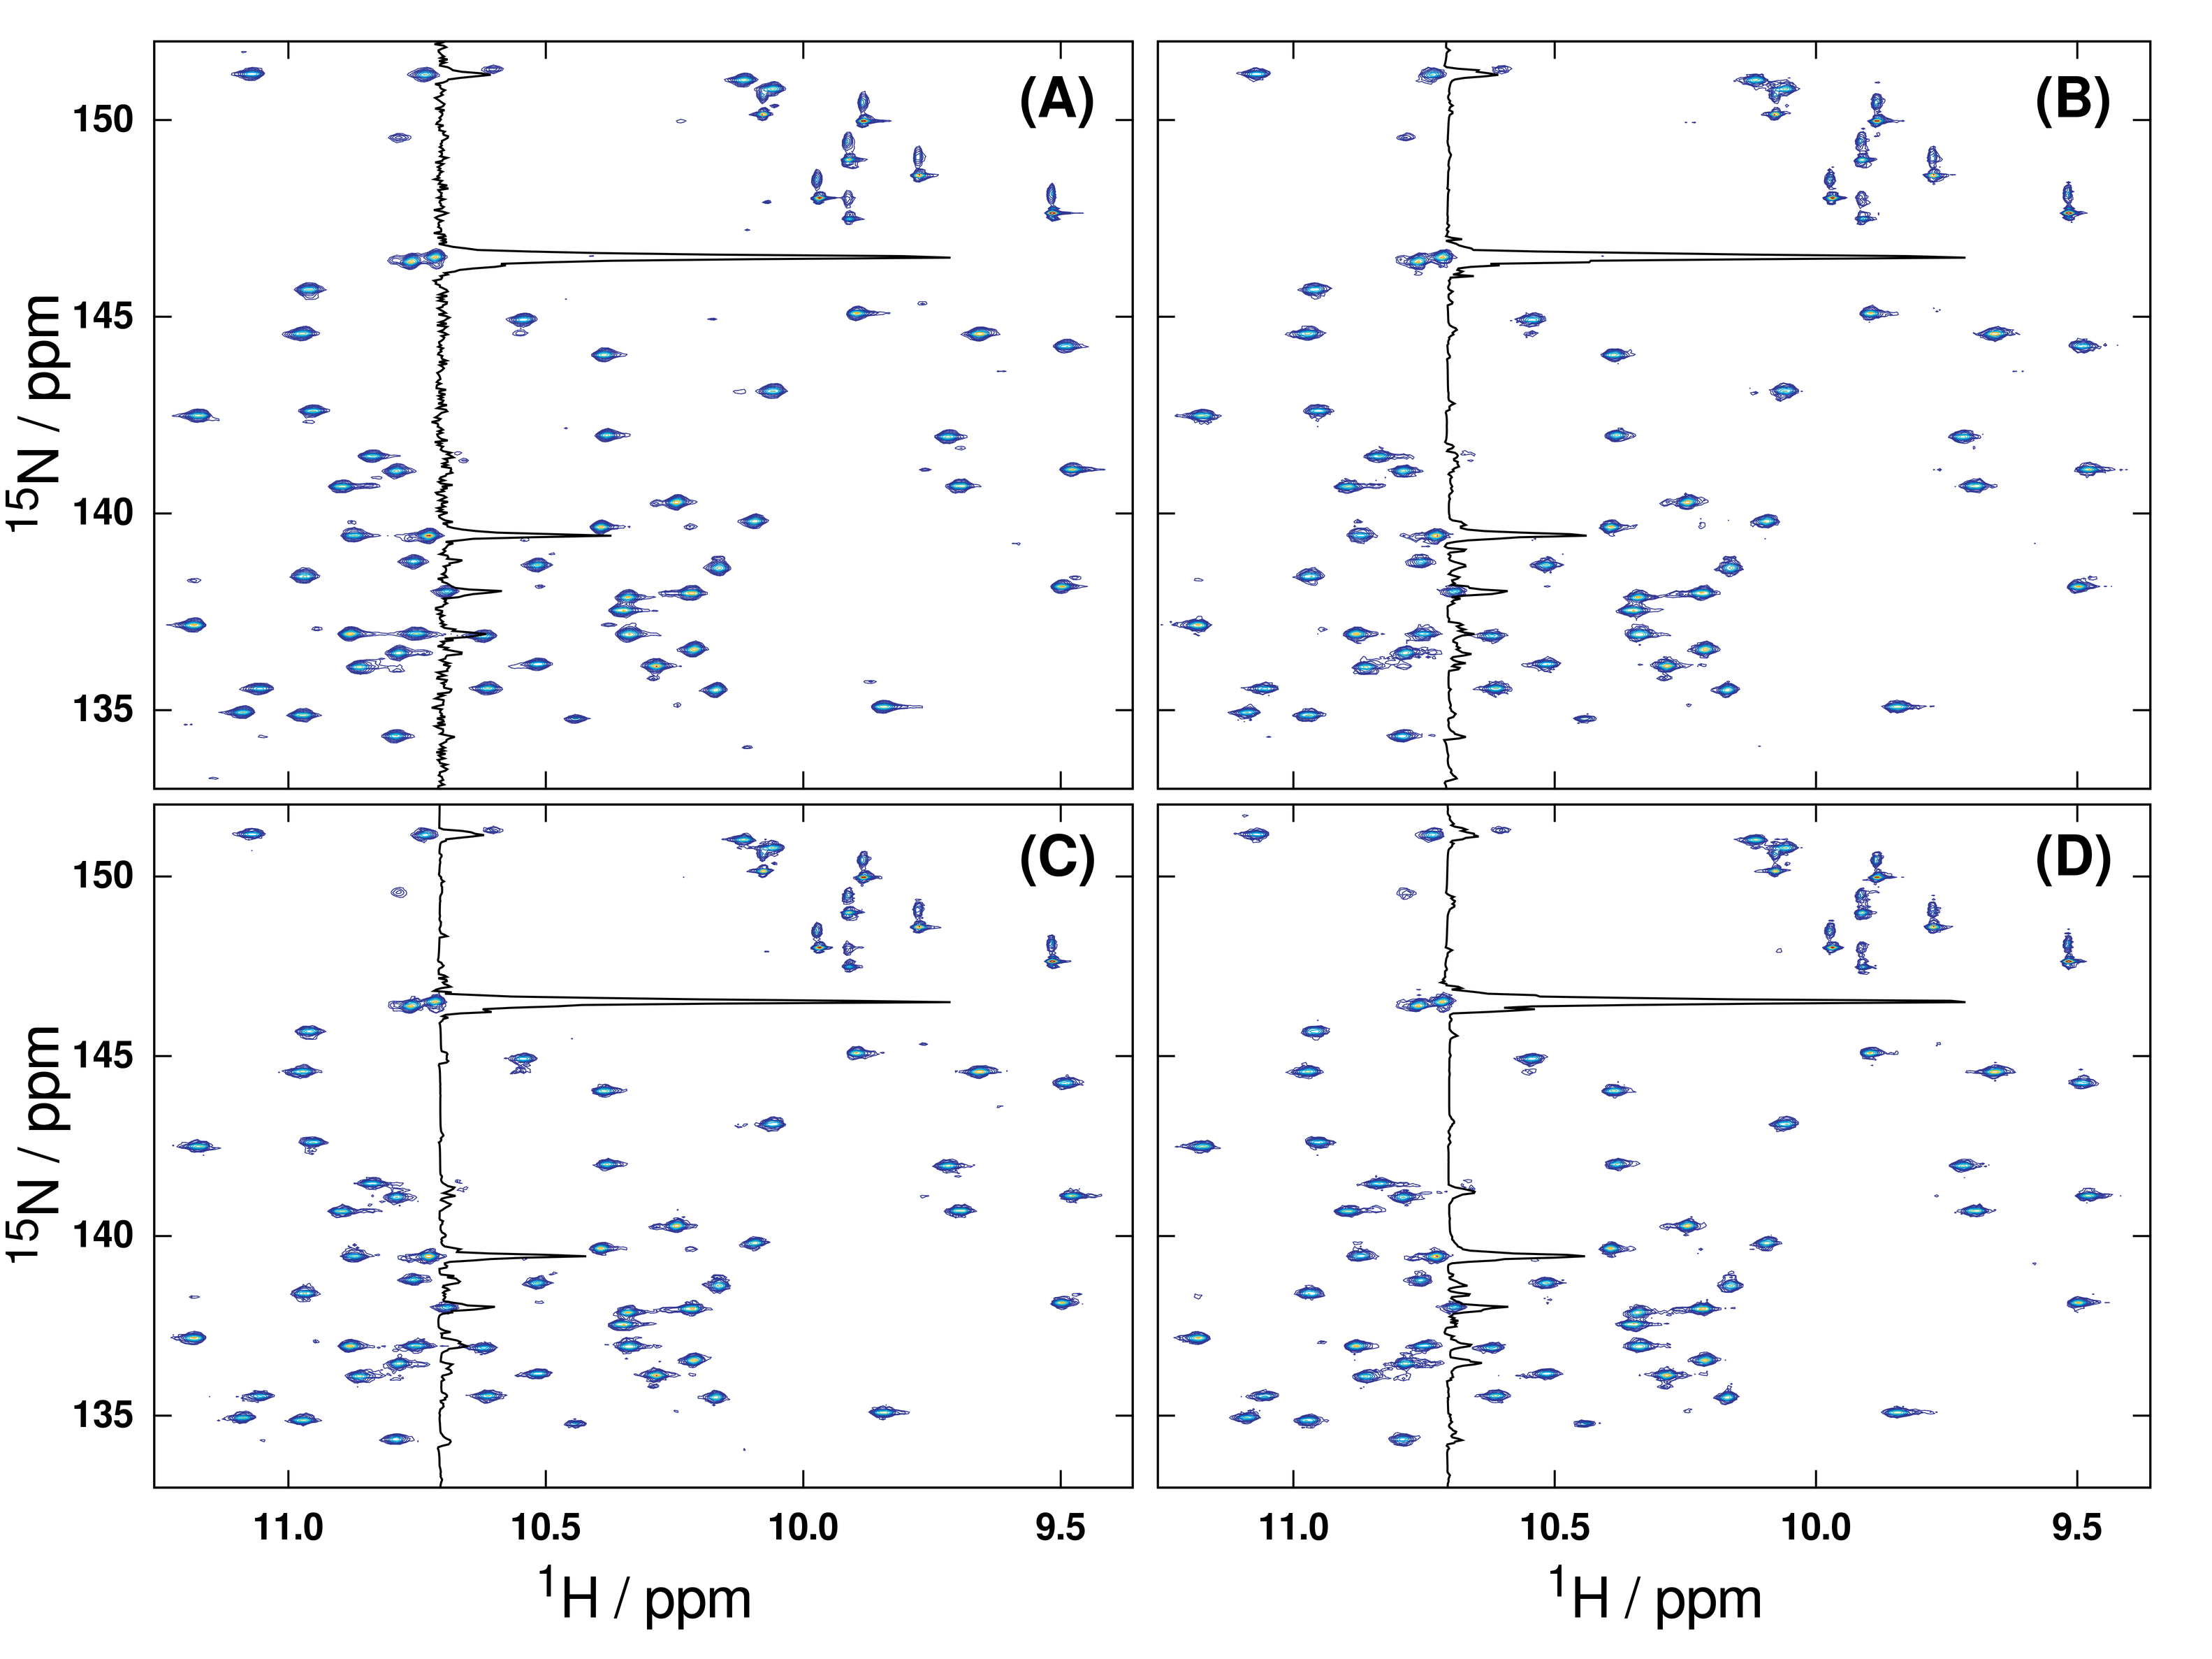
\includegraphics[width=6in]{figs/dgs/06-hsqc.png}
\caption
      [Comparison of HSQC Spectral Reconstructions.]{
  {\bf Comparison of HSQC Spectral Reconstructions.}
  \\
  Uniformly sampled ({\bf A}) and IST reconstructed ({\bf B--D}) 2D \hnnmr{}
  HSQC spectra of ubiquitin, indicating nearly equivalent performance of all
  three gap sampling methods at low (5\%) sampling density. Spectra shown in
  ({\bf B}) through ({\bf D}) were reconstructed from nonuniformly subsampled
  copies of ({\bf A}) using Poisson-gap ({\bf B}), sine-gap ({\bf C}), and
  sine-burst ({\bf D}) schedules, respectively. All spectra are plotted with
  identical contour levels.
}
\label{figure.2.6}
\end{figure}

\subsection{Spectral Data Collection}

\begin{doublespace}
A high-resolution 2D \hnnmr{} HSQC NMR spectrum was collected at a temperature
of 298.0 K on a sample of uniformly [\nnmr{}, \cnmr{}]-labeled ubiquitin in
aqueous phosphate buffer at pH 6.5. Data were acquired on a Bruker Avance
III HD 700 MHz spectrometer equipped with a 5 mm inverse quadruple-resonance
(\hnmr{}, \cnmr{}, \nnmr{}, \pnmr{}) cryoprobe with cooled \hnmr{} and \cnmr{}
channels and a $z$-axis gradient. A 2D gradient-enhanced \hnnmr{} HSQC spectrum
with improved sensitivity \cite{kay:jacs1992,palmer:jmr1991} was collected with
16 scans and 32 dummy scans over a uniform grid of 2,048 and 1,024 complex
points along the \hnmr{} and \nnmr{} dimensions, respectively. Spectral widths
were set to 3,293$\pm$4,209 Hz along \hnmr{} and 8,514$\pm$1,419 Hz along
\nnmr{}. The spectrum was windowed with a squared-cosine function,
Fourier-transformed and phase-corrected along \hnmr{} to produce a
half-transformed spectrum for IST reconstruction analysis (vide infra),
and subsequently windowed and Fourier-transformed along \nnmr{} to yield the
``true'' uniformly sampled 2D \hnnmr{} HSQC spectrum.
\figref{2.6}{Figure 2.6A} compares the true HSQC spectrum with
representative IST reconstructions after subsampling by
Poisson-gap, sine-gap and sine-burst schedules.
\end{doublespace}

\begin{figure}[ht!]
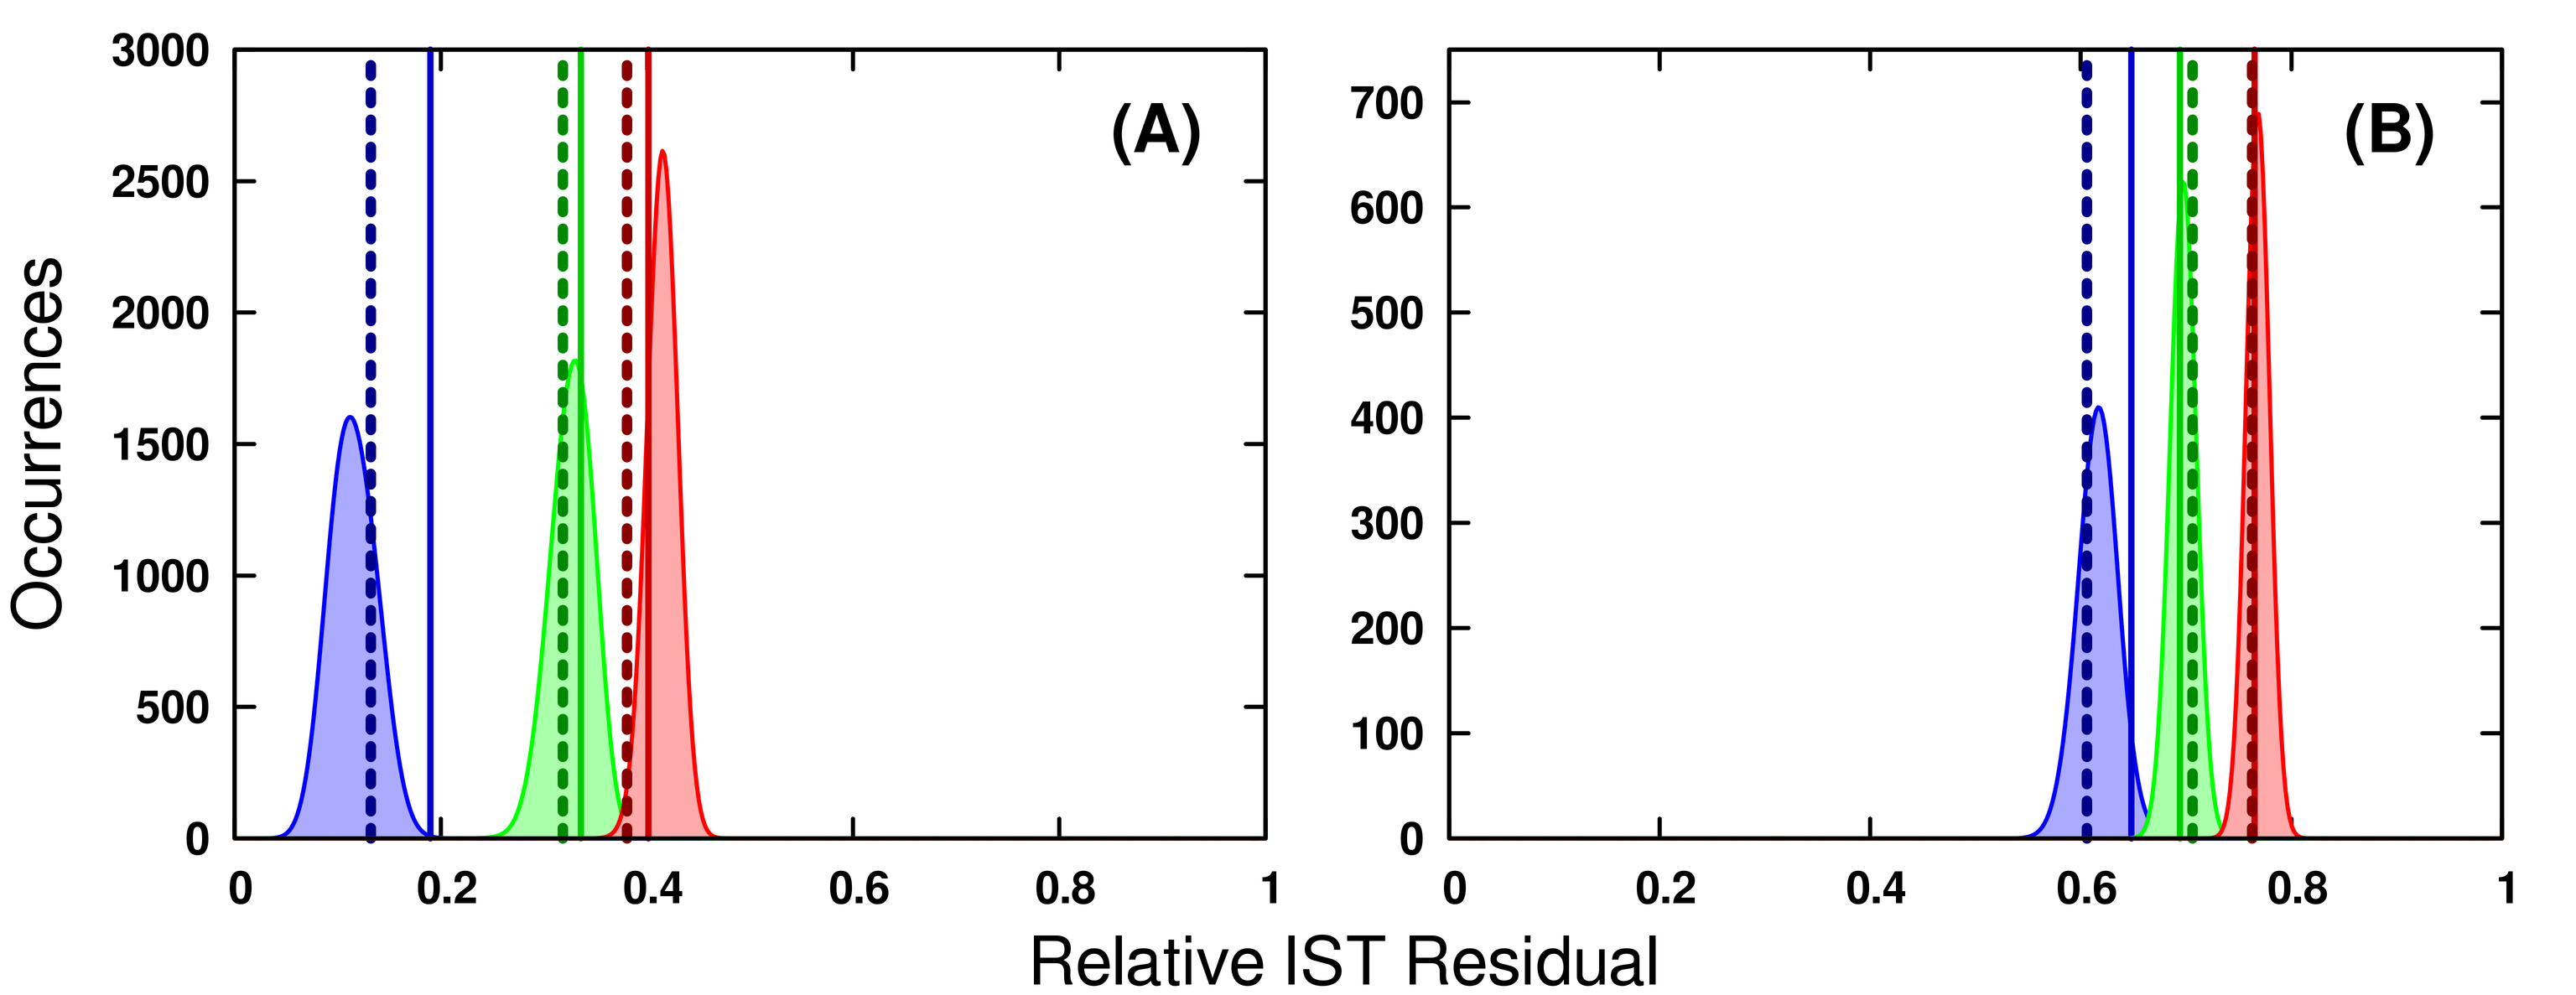
\includegraphics[width=6in]{figs/dgs/07-residuals.png}
\caption
      [Relative IST Reconstruction Residuals.]{
  {\bf Relative IST Reconstruction Residuals.}
  \\
  Iterative soft thresholding reconstruction $\ell_2$ residuals of ({\bf A})
  simulated noise-free decays and ({\bf B}) 2D \hnnmr{} HSQC slices from
  one-dimensional Poisson-gap schedules having sampling densities of
  30\% (blue), 10\% (green) and 5\% (red). Residuals of sine-gap and sine-burst
  schedules are shown as solid and dashed vertical lines, respectively.
}
\label{figure.2.7}
\end{figure}

\subsection{Computation of Performance Metrics}

\begin{doublespace}
All computational analyses were performed in GNU Octave 3.6 \cite{eaton2008}
using routines currently available in the open-source MVAPACK toolbox for
NMR chemometrics \cite{worley:acscb2014}. Impulse sets were generated for
each constructed schedule by setting sampled grid points to one and skipped
grid points to zero. At each sampling density and grid size for which schedules
were created, point-spread functions were calculated by discrete Fourier
transformation of each schedule's impulse set. Point-spread functions for
schedules built on two-dimensional grids are shown for each sampling density
in \figref{2.5}{Figure 2.5}. For one-dimensional schedules, reconstruction
residuals were computed for a noise-free synthetic free induction decay
containing a single frequency component. The synthetic decay had a normalized
frequency and decay rate of 0.04 and 0.002, respectively. The decay was
resampled according to each schedule and reconstructed with 400 iterations
of Iterative Soft Thresholding (IST) at a threshold level
of 98\% \cite{hyberts:jbnmr2012}. Following reconstruction, the residual
was calculated using the $\ell_2$-norm of the differences between the
true and reconstructed signals. \figref{2.7}{Figure 2.7A} shows the
distributions of IST reconstruction residuals for Poisson-gap, sine-gap and
sine-burst schedules. Reconstructions of the half-transformed HSQC were also
performed after nonuniformly subsampling using sine-gap schedules, sine-burst
schedules, and a subset ($N$ = 10,000) of the generated Poisson-gap schedules.
\figref{2.7}{Figure 2.7B} shows IST reconstruction residuals computed
from the HSQC spectrum.
\end{doublespace}

\begin{table}[h!]
\caption{Peak-picking Performance Figures from IST-reconstructed HSQC Spectra.}
\begin{center}
\begin{tabular}{l l | l l l l l l}
  \hline
  {\bf Method} & & {\bf Matched}       & {\bf Lost}     & {\bf Gained} &
                   $\boldsymbol{\rho}$ & $\mathbf{d_H}$ & $\mathbf{d_N}$ \\
  \hline
     & 30\% & 92/99 & 7/99 &  2 & 0.9736 & 0.003064 & 0.006165 \\
  PG & 10\% & 96/99 & 3/99 &  6 & 0.9692 & 0.003451 & 0.011702 \\
     &  5\% & 94/99 & 5/99 & 32 & 0.9751 & 0.003034 & 0.012806 \\
  \hline
     & 30\% & 93/99 & 6/99 &  3 & 0.9704 & 0.003184 & 0.005882 \\
  SG & 10\% & 96/99 & 3/99 & 13 & 0.9732 & 0.002801 & 0.011357 \\
     &  5\% & 97/99 & 2/99 & 31 & 0.9630 & 0.003450 & 0.014585 \\
  \hline
     & 30\% & 91/99 & 8/99 &  3 & 0.9820 & 0.003319 & 0.008370 \\
  SB & 10\% & 97/99 & 2/99 & 13 & 0.9820 & 0.003045 & 0.012806 \\
     &  5\% & 97/99 & 2/99 & 45 & 0.9575 & 0.003587 & 0.016998 \\
\end{tabular}
\end{center}
\end{table}

\subsection{Generation of Peak-picking Statistics}

\begin{doublespace}
For each 2D \hnnmr{} HSQC spectrum of ubiquitin reconstructed via IST at each
sampling density and each sampling method, a set of quality statistics was
computed (Table 2.1). Peak lists were generated using the
\verb peakHN.tcl  utility provided by NMRPipe \cite{delaglio:jbnmr1995}, with
a minimum intensity threshold of $3.0 \times 10^7$. Then, a greedy algorithm
was used to generate a maximum-cardinality bipartite matching between the peak
list of each reconstructed spectrum and the peak list of the true spectrum.
Chemical shift windows of 0.015 ppm and 0.08 ppm were used along the \hnmr{}
and \nnmr{} dimensions, respectively, during matching. The numbers of peaks
matched, lost and gained in the reconstructed spectra, relative to the true
spectrum, were all counted. Lost peaks were any picked peaks in the true
spectrum that had no match in the reconstruction. Gained peaks were any
picked peaks in the reconstruction with no partner in the true spectrum.
The intensities of all matched peaks in each reconstruction were then
compared against their true intensities through the computation of a Pearson
correlation coefficient, $\rho$, which effectively summarizes the linearity
of the reconstruction algorithm as a function of sampling schedule. Finally,
root-mean-square chemical shift deviations of all matched peaks along the
\hnmr{} dimension ($d_H$) and the \nnmr{} dimension ($d_N$) were also
computed.
\end{doublespace}

\begin{SCfigure}
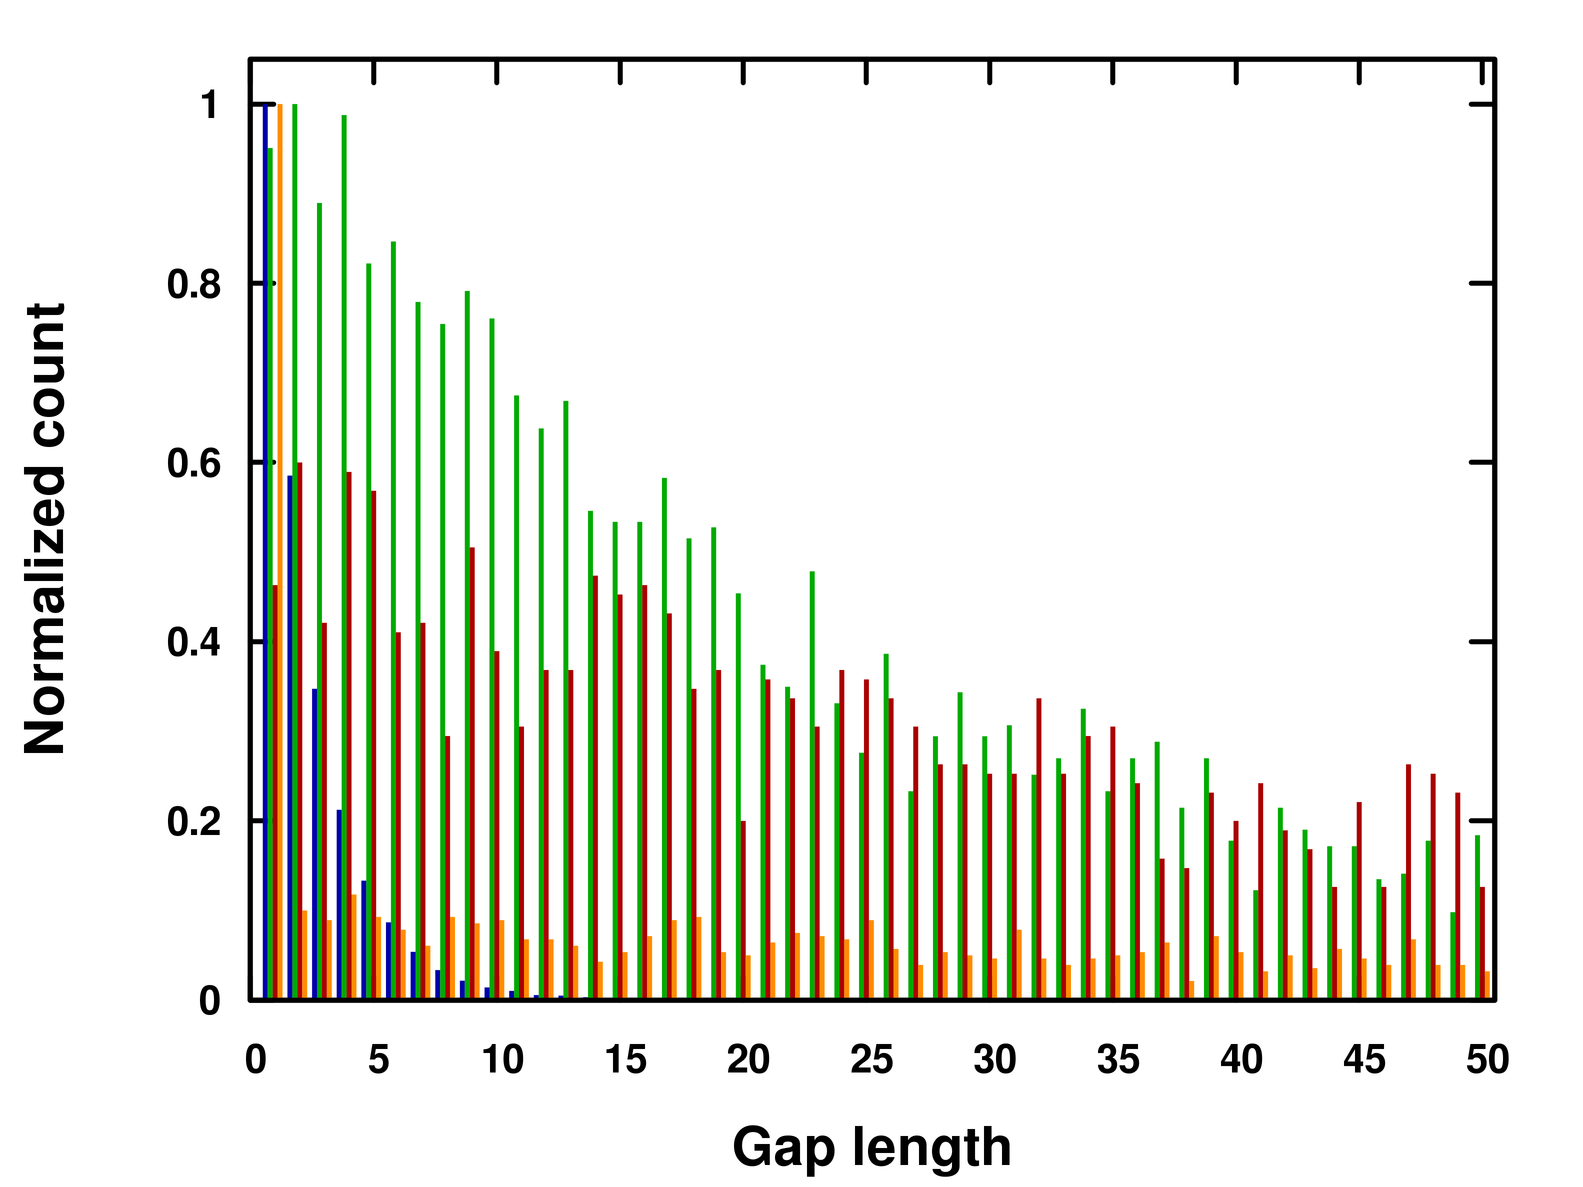
\includegraphics[width=3.25in]{figs/dgs/08-rejhist.png}
\caption
      [Gap Length Histograms from Rejection Sampling.]{
  {\bf Gap Length Histograms from Rejection Sampling.}
  \\
  Normalized histograms of gap lengths at various points in an ensemble of
  100,00 sampling schedules generated by rejection sampling from the
  Poisson-gap expectation sampling distribution (equation 2.11). Bars
  shown in blue, green, red and orange represent the gap length histograms
  at $\theta$ equal to 0.0098, 0.24, 0.73 and 0.88, respectively. Examination
  of these histograms clearly indicates that the schedules generated by
  rejection sampling are \emph{not} Poisson-gap schedules.
}
\label{figure.2.8}
\end{SCfigure}

\subsection{Analysis of Sampling Distributions}

\begin{doublespace}
Expectation sampling distributions were also generated from the set of
Poisson-gap schedules by averaging their resulting impulse sets.
\figref{2.2}{Figure 2.2} shows the expectation sampling distributions
for one-dimensional schedules having different sampling densities, and
\figref{2.3}{Figures 2.3} and \figref{2.4}{2.4} show the distributions
for two-dimensional schedules having the same densities. The heavy bias
towards early time points in Poisson-gap sampling is reaffirmed in all
figures. Sampling distributions were also computed via equations
2.11 and 2.12 for comparison to the distributions obtained by averaging
multiple impulse sets (\figref{2.2}{Figures 2.2} and \figref{2.3}{2.3}).
To verify that fully random sampling from equation 2.11 and gap sampling
from $g_{PG}$ are not equivalent, 100,000 sampling schedules were generated
by rejection sampling 51 grid points from equation 2.11 at $\Lambda=62.9$
and $N=1024$, and histograms of the gap lengths at each grid point were
computed (\figref{2.8}{Figure 2.8}). If the two methods were indeed
equivalent, one would expect the histograms in \figref{2.8}{Figure 2.8} to
resemble Poisson distributions.
\end{doublespace}

\subsection{Average Poisson-gap Sequences}

\begin{doublespace}
For \figref{2.1}{Figure 2.1}, each schedule
$\{x_1^{(m)}, x_2^{(m)},\dots, x_n^{(m)}\}$ in
the generated ensemble of $M$ (here, $M$ = 50,000)
one-dimensional Poisson-gap schedules was averaged
on a term-by-term basis:
\begin{equation}
\langle x_i \rangle = \frac{1}{M} \sum_{m=1}^M x_i^{(m)}
\end{equation}
to produce the average Poisson-gap schedule
$\{\langle x_1 \rangle, \langle x_2 \rangle,\dots, \langle x_n \rangle\}$.
Similar procedures were performed to compute the standard deviation of the
Poisson-gap ensemble. Deterministic sampling schedules with a 1x exponential
bias were computed according to procedures outlined by
Eddy et al. \cite{eddy:jmr2012}. Relative errors
(\figref{2.1}{Figure 2.1}) between a given
sine-gap schedule $\{y_1, y_2,\dots, y_n\}$ and average Poisson-gap schedule
were computed by a term-by-term subtraction of one schedule from the other,
followed by a division by the average Poisson-gap terms:
\begin{equation}
\Delta_i = \frac{y_i - \langle x_i \rangle}{\langle x_i \rangle}
 \quad \forall i \in \{1,2,\dots, n\}
\end{equation}

Relative errors between the deterministic exponential schedules and the
average Poisson-gap sequence were similarly computed.
\end{doublespace}

\begin{SCfigure}
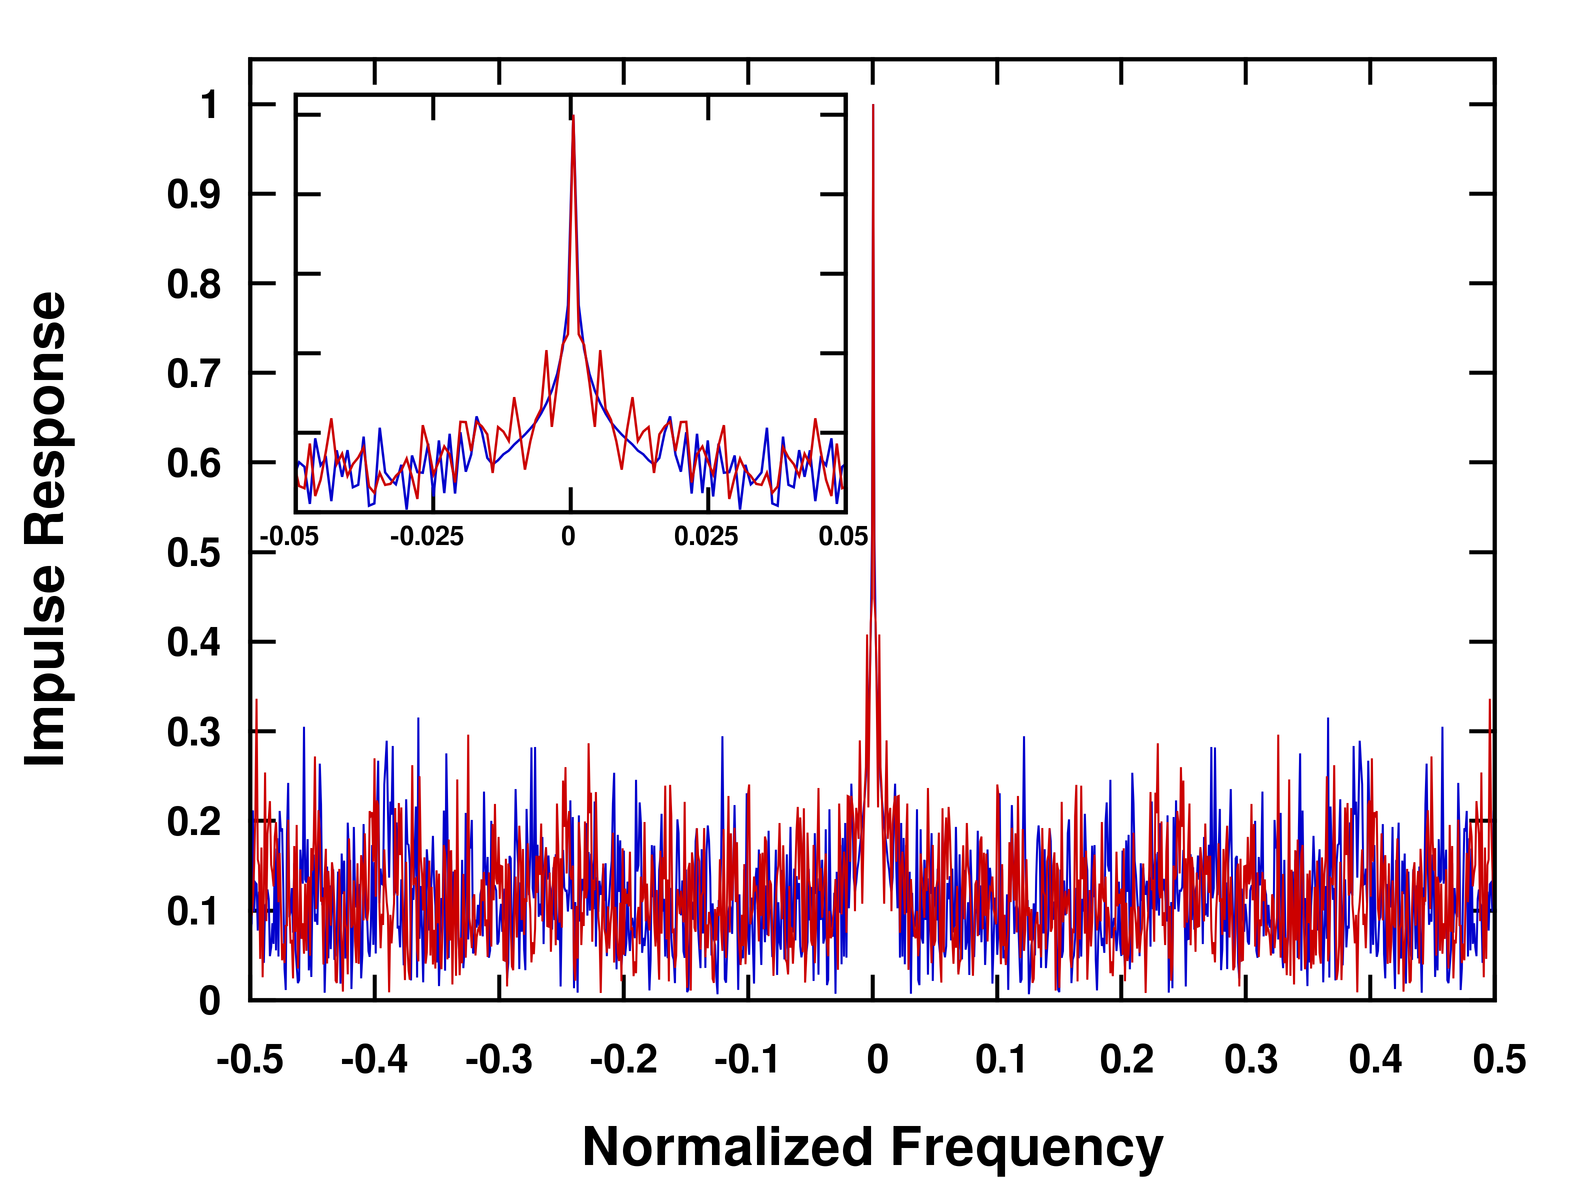
\includegraphics[width=3.25in]{figs/dgs/09-spurs.png}
\caption
      [Introduction of Spurs by Squared-sine Modulation.]{
  {\bf Introduction of Spurs by Squared-sine Modulation.}
  \\
  Impulse response functions (IRFs) of sine-gap (blue) and sine-burst (red)
  sampling schedules at 5\% density, demonstrating the appearance of
  low-frequency spurs induced by burst augmentation of the gap equation.
}
\label{figure.2.9}
\end{SCfigure}

\section{Results}

\begin{doublespace}
While at first glance, the deterministic schedule constructed using $g_{SG}$
in \figref{2.5}{Figure 2.5} may appear unrelated to the Poisson-gap
schedule, it is in fact a realization of Poisson-gap sampling in which all
random draws from the underlying Poisson distribution have resulted in the
expected value. This fact is corroborated by the corresponding point-spread
functions, which closely resemble those of the stochastic example at 30\% and
10\% sampling density. Reconstruction residuals from IST
(\figref{2.7}{Figure 2.7}) also reveal a high
similarity between the deterministic sine-gap and stochastic Poisson-gap
schedules at 30\% and 10\% density. However, the sine-gap PSF becomes less
comparable to that of Poisson-gap at low sampling densities, where the
benefits of employing random deviates are more apparent. It is worth noting
that the striking appearance of sampling artifacts in the sine-gap PSF is a
consequence of the log-scaled color gradient used in \figref{2.5}{Figure 2.5},
which was necessary in order to visually expose very low-intensity artifacts.
\\\\
The addition of burst augmentation in the form of $g_{SB}$ produces a slight
improvement in all reconstruction residuals with respect to $g_{SG}$ and
$g_{PG}$. Artifacts arising from regularity in $g_{SG}$-based schedules at
low sampling densities are diminished by burst augmentation, resulting in
point-spread functions that more closely resemble those from Poisson-gap
sampling. This reduction of artifacts by burst augmentation comes at a small
cost, at low-frequency spurs are introduced into the sine-burst point-spread
function (\figref{2.9}{Figure 2.9}) by modulating the gap equation.
However, these spurs are low in magnitude and only readily apparent at very
low (5\%) sampling density. Furthermore, IST residuals of sine-burst schedules
(\figref{2.7}{Figure 2.7}, dashed lines) are generally lower than
those of sine-gap schedules, and appear to improve relative to the mean
residuals from Poisson-gap schedules as sampling density is decreased.
Therefore, while sine-gap sampling is a valuable tool for understanding
the nature of Poisson-gap sampling, it is clearly bested in performance
by sine-burst sampling as global sampling density is decreased.
\\\\
The trade-off between minimizing the length of all gaps in a schedule, as
Poisson-gap strives to do, and minimizing the effective dwell time, as in
burst-mode sampling, is apparent by examination of gap lengths produced by
each method (\figref{2.10}{Figure 2.10}). As advertised, sine-burst
sampling schedules have decreased median gap lengths with respect to both
sine-gap and Poisson-gap schedules (\figref{2.10}{Figure 2.10A}),
at the expense of slightly increased maximum gap lengths
(\figref{2.10}{Figure 2.10B}). Rather remarkably, sine-gap schedules
have lower maximum gap lengths than their stochastic Poisson-gap cousins
\emph{and} sine-burst schedules, which reinforces the concept that the
addition of \emph{any} mechanism to reduce the greatest common factor of
the gap lengths between sampled points with force an increase in the
largest gap between points.
\end{doublespace}


\begin{figure}[ht!]
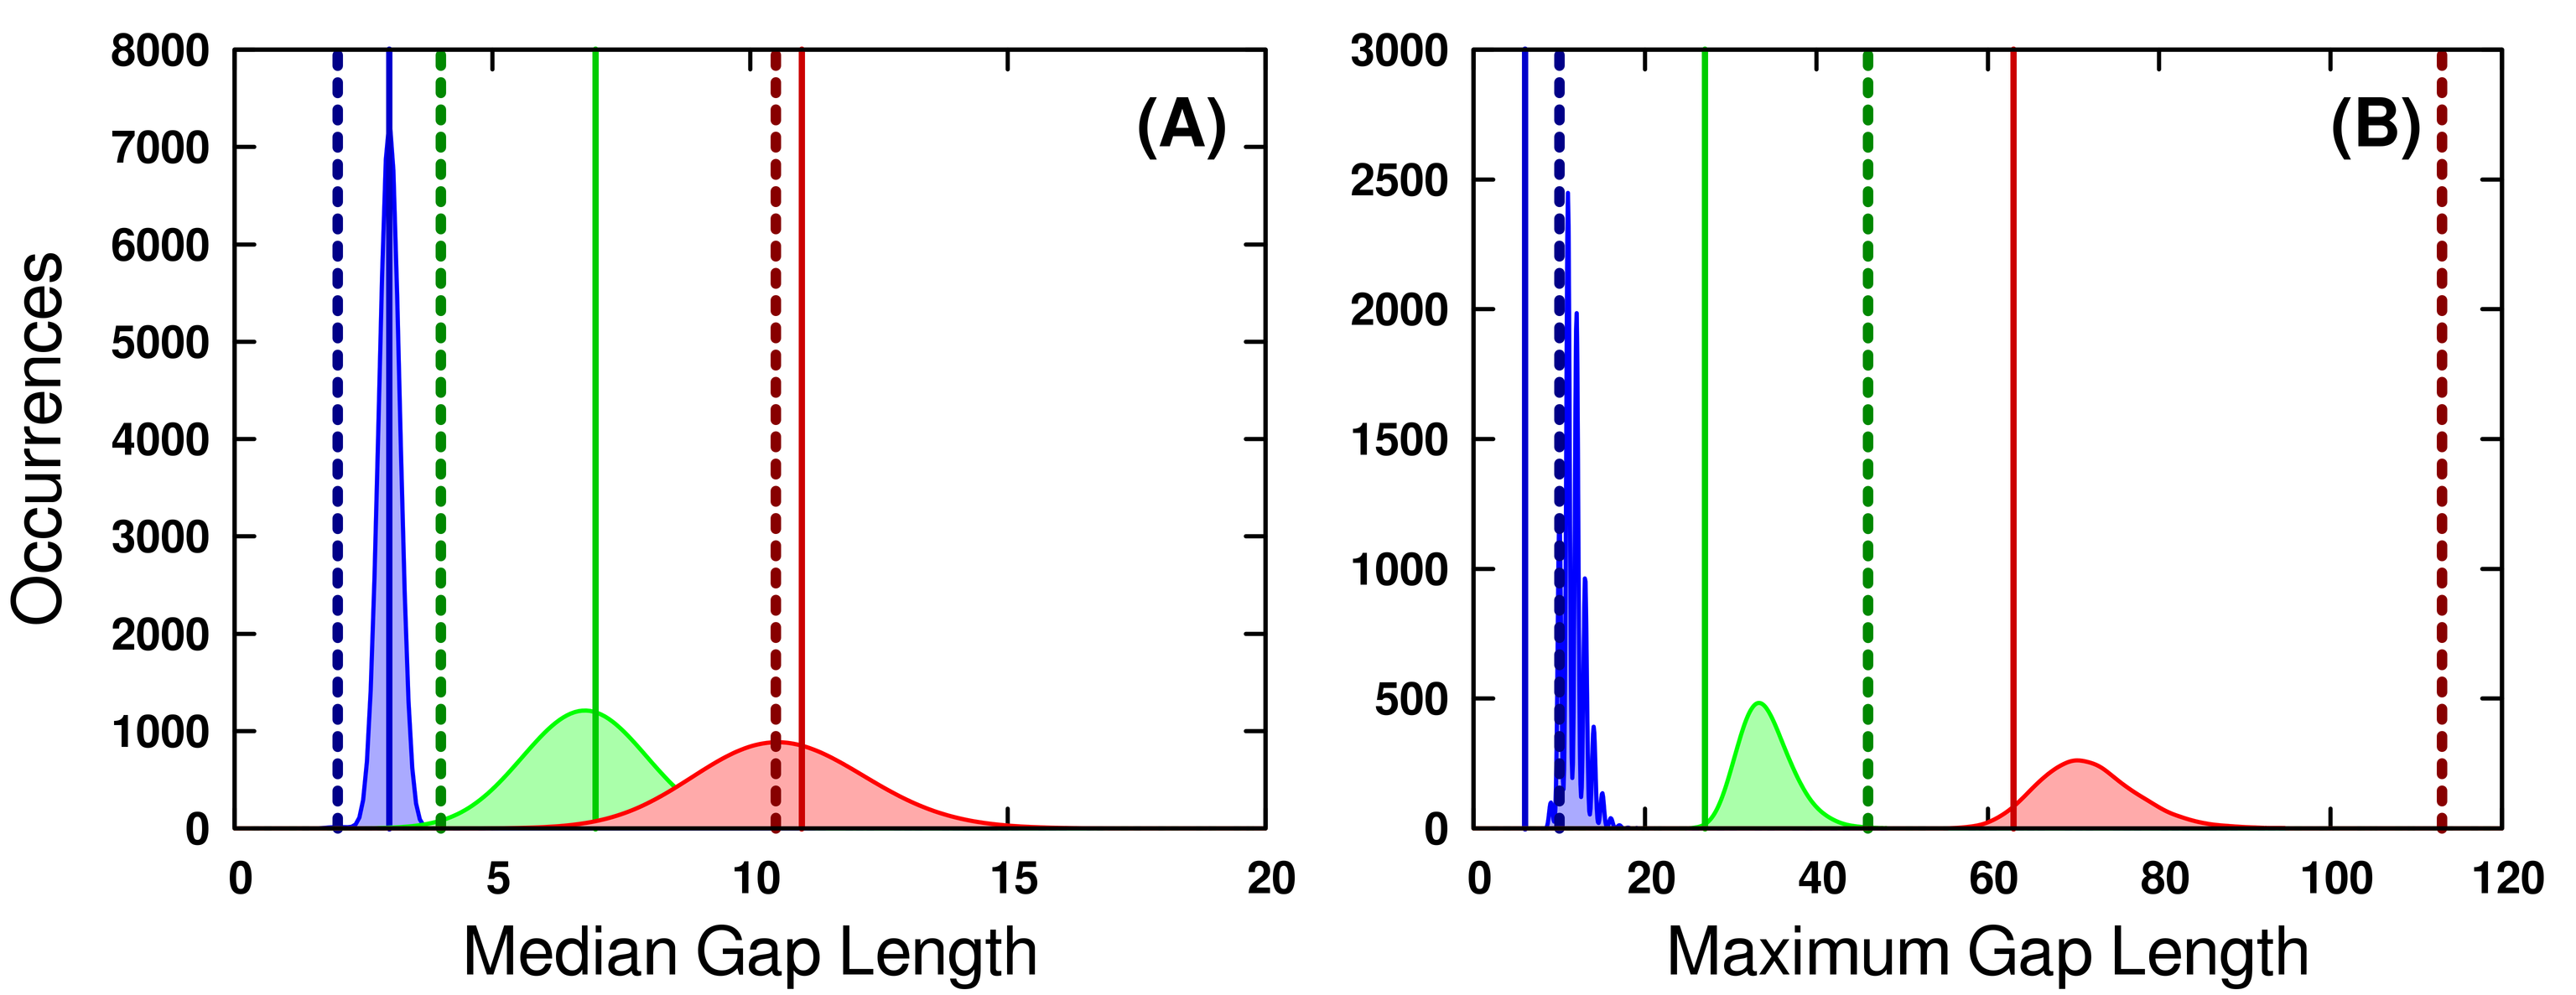
\includegraphics[width=6in]{figs/dgs/10-gaps.png}
\caption
      [Summary of Gap Lengths for all Sampling Methods.]{
  {\bf Summary of Gap Lengths for all Sampling Methods.}
  \\
  Distributions of median ({\bf A}) and maximum ({\bf B}) gap lengths from
  one-dimensional Poisson-gap schedules having sampling densities of
  30\% (blue), 10\% (green) and 5\% (red). Gap lengths of sine-gap and
  sine-burst schedules are shown as solid and dashed vertical lines,
  respectively. The gap lengths resulting from burst augmentation of the
  sine-gap equation have markedly decreased median values at the expense
  of increased maximum values, relative to sine-gap and Poisson-gap schedules.
}
\label{figure.2.10}
\end{figure}

\section{Discussion and Conclusions}

\begin{doublespace}
This chapter has shown that Poisson-gap sampling is a single instance in a
class of gap sampling methods, which may or may not be defined stochastically.
Using the well-defined gap sampling algorithm, two novel deterministic sampling
methods have been described: sine-gap and sine-burst sampling. Neither of
these new methods relies on random deviates, and both have comparable
performance to Poisson-gap sampling according to IST reconstruction residuals.
From a practical perspective, Poisson-gap, sine-gap and sine-burst sampling
methods produced nearly equivalent HSQC spectral reconstructions
(\figref{2.6}{Figure 2.6}) that yielded essentially identical
information (chemical shifts, peak
intensities) as highlighted in Table 2.1. For the practicing spectroscopist,
this equates to the ability to nonuniformly sample at the performance level
of Poisson-gap, without specifying a pseudorandom seed. Gap sampling is a
flexible and attractive alternative to traditional probabilistic sampling
methods that use probability densities to define the local sampling density
over a Nyquist grid. In effect, gap sampling approaches the problem of local
sampling density from the opposite direction of probabilistic sampling by
defining the distances \emph{between} samples on the grid. This chapter also
holds a brief derivation of the mathematical connection between stochastic
gap equations and their expectation sampling distributions, which allows for
direct visualization of the grid-point weighting produced by a given gap
equation. While these expectation sampling distributions are useful in
describing the sampling behavior of a stochastic gap equation, they do not
provide a means of converting a gap-based sampling method into a fully random
sampling method. In other words, it has been shown that any method of
constrained random sampling using a gap equation is inequivalent to fully
random sampling from its corresponding expectation sampling distribution.
\\\\
Finally, burst augmentation provides a concrete example of how deterministic
gap sampling may be tuned to behave in a similar fashion to pseudorandom
numbers. At first glance, the third row of \figref{2.5}{Figure 2.5} would
appear to have been generated stochastically, but it is a consequence of the
squared-sine modulation term in $g_{SB}$. It has historically been true that
stochastically generated sampling schedules produced fewer prominent artifacts
than deterministic methods such as radial or spiral sampling, due to high
regularity of the latter schemes. However, pseudorandom variates are
not required for effective sampling artifact suppression. Furthermore,
while most pseudorandom number generators are indeed deterministic for a
given seed value, this determinism is \emph{inherently different} from the
determinism offered by sine-gap and sine-burst sampling. By design, any
parameters (e.g. reconstruction residuals) measured from pseudorandomly
generated sampling schedules will not be smoothly varying -- and therefore
optimizable -- functions of their random seed value. As a consequence, no
absolute guarantee of spectral quality is provided to the spectroscopist
employing pseudorandom sampling schedules, even if the relative difference
in quality between the best- and worst-performing Poisson-gap seed values
is small at sampling densities above 10\%. This problem with seeds has
already been recognized: Poisson-gap and jittered sampling methods are, in
fact, two separate attempts at minimizing -- but not removing -- the effect
of seed values on schedule performance
\cite{hyberts:jacs2010,kazimierczuk:jmr2007,mobli:jmr2015}. Deterministic
gap sampling completely frees the user from specifying an arbitrary seed
value, and provides a highly general framework that enables further
investigation into which features of NUS schedules yield higher-quality
reconstruction results.
\\\\
The C implementations of Poisson-gap, sine-gap and sine-burst sampling are
free and open source software, and are available for download at
\url{http://bionmr.unl.edu/dgs.php}. The programs are highly portable and
C99 compliant, so they may be compiled on any modern operating system. An
online schedule generation tool is also provided at the same address for
rapid generation of one-, two- and three-dimensional NUS schedules suitable
for direct use on Bruker or Agilent spectrometers. As defined and implemented,
the recursive schedule generation algorithm is not limited to any number of
grid dimensions. However, the online tool has been hard-limited to 3D grids
to minimize server load.
\end{doublespace}

\bibliographystyle{abbrv}
\bibliography{bworley}



\chapter{Multivariate Analysis in Metabolomics}

\begin{quote}
{\it Essentially, all models are wrong, but some are useful.}
\\\\
 -- George E. P. Box
\end{quote}

\section{Introduction}

\begin{doublespace}
The applications of chemometrics are as broad as the field of chemistry itself,
but one particularly challenging subdiscipline of bioanalytical chemistry --
known as ``metabolomics'' -- has recently renewed interest in the use of
chemometrics \cite{worley:cmb2013}. Indeed, the chemical complexity of
systems studied by metabolomics {\it necessitates} the use of chemometric
techniques: if metabolomics were a nail, chemometrics would surely be a hammer.
\\\\
Metabolomics is defined \cite{lindon:cmr2000} as ``the quantitative
measurement of the multiparametric metabolic response of living systems to
pathophysiological stimuli or genetic modification.'' Such a definition implies
that metabolomics studies offer the finest-grained detail available in the
nascent field of systems biology: a molecular-level convolution of all upstream
genomic, transcriptomic and proteomic responses of an organism to a given
stimulus or change
\cite{kell:opin2004,trethewey:opin2001,weckwerth:arpb2003}. Metabolites
are the end product of all cellular processes, and their in vivo
concentrations are a direct result of enzymatic activity. While a change in the
expression level of a protein or its coding gene may not necessarily correlate
directly with the activity of that protein, alterations in metabolite
concentrations {\it are} the consequence of altered activity
\cite{terkuile:febs2001}. Thus, metabolites are more proximal to a
phenotype or disease state than either genetic or proteomic information. The
richness of phenotypic information offered by metabolomics has been leveraged
to identify disease biomarkers
\cite{gebregiworgis:cchts2012,vinayavekhin:acscb2010}, to aid in
the drug discovery process \cite{powers:mrc2009,wilcoxen:eodd2010}, and to
study plants \cite{hall:pcell2002}, bacteria
\cite{zhang:jiomic2013,tang:cgen2011}, nutrition
\cite{mcniven:jnb2011}, and the environment
\cite{bundy:metab2009}, among numerous other applications
\cite{baker:nmeth2011}.
\\\\
The rich information promised by metabolomics does not come without a price,
and metabolomics experiments are plagued with difficulty. The number of
small-molecule metabolites in a biofluid, cell lysate, tissue or organ differs
wildly depending on the organism studied, ranging from several hundred to
hundreds of thousands \cite{dunn:trac2005}. While databases of commonly
encountered metabolites have been compiled
\cite{wishart:nar2007,cui:nbiot2008,kind:anchem2009}, they are by no
means complete. Therefore, it is common to encounter unknown signals during
data analysis, complicating the interpretation of metabolic changes between
experimental groups. Metabolite identification is further complicated by a
lack of NMR or mass spectral reference information for known metabolites.
Finally, the diversity of chemical and physical properties of metabolites
makes true simultaneous quantitation of all metabolites present in a system
unattainable with current instrumental capabilities
\cite{lindon:cmr2000,dunn:trac2005,dettmer:msr2007}. As an illustration,
due to the limited molecular mass distribution of the metabolome, comprehensive
metabolomic analyses by mass spectrometry generally require the prefixing of
one or more chromatographic separations prior to analyte ionization
\cite{kell:opin2004,viswanadhan:acsccc2011}.
\\\\
The extraction of information from data in metabolomics experiments is further
complicated by the inherent variability present within each sample. Every
single cell, tissue, organ or organism is fundamentally unique
\cite{rubakhin:nmeth2011}, despite any features (disease state, drug
treatment, {\it etc.}) it may have in common with others of its kind. Thus,
the differentiation between two experimental groups in a metabolomics
experiment requires the identification of relatively few defining or
discriminating chemical features against a large, complex background of
metabolites \cite{wishart:nar2007}. Ideally, these few chemical features
may be identified as a unique set of metabolites that are directly related to
the defining biochemical states of each experimental group. Unfortunately, all
biological systems are easily perturbed by experimental or environmental
factors, including age, gender, diet, cell growth phase, nutrient availability,
pH and temperature \cite{tyagi:ijpsrr2010,zhang:jiomic2013}. Variations in
sample handling procedures, including cell lysis, metabolic quenching,
metabolite extraction and sample storage can also introduce further variability
into the measured data. Finally, variations in signal position, intensity and
shape may manifest from instrumental instabilities on a per-sample basis.
Each of these numerous sources of sample variability increases the magnitude of
$\mathbf{E}$ in any chemometric model that may be applied to the data
(cf. \hyperlink{section.1.1}{Section 1.1}), which decreases the statistical
validity of $f(\mathbf{D})$. Therefore, the design of experiments and analysis
of data in metabolomics requires robust methodologies in order to expose
underlying chemical trends from highly complex systems in the form of
statistically valid mathematical models. This chapter describes the theory
and best practices of chemometric analyses of data produced by metabolomics
experiments, with a focus on 1D \hnmr{} and 2D \hcnmr{} NMR datasets.
\end{doublespace}

\begin{figure}[ht!]
\begin{center}
  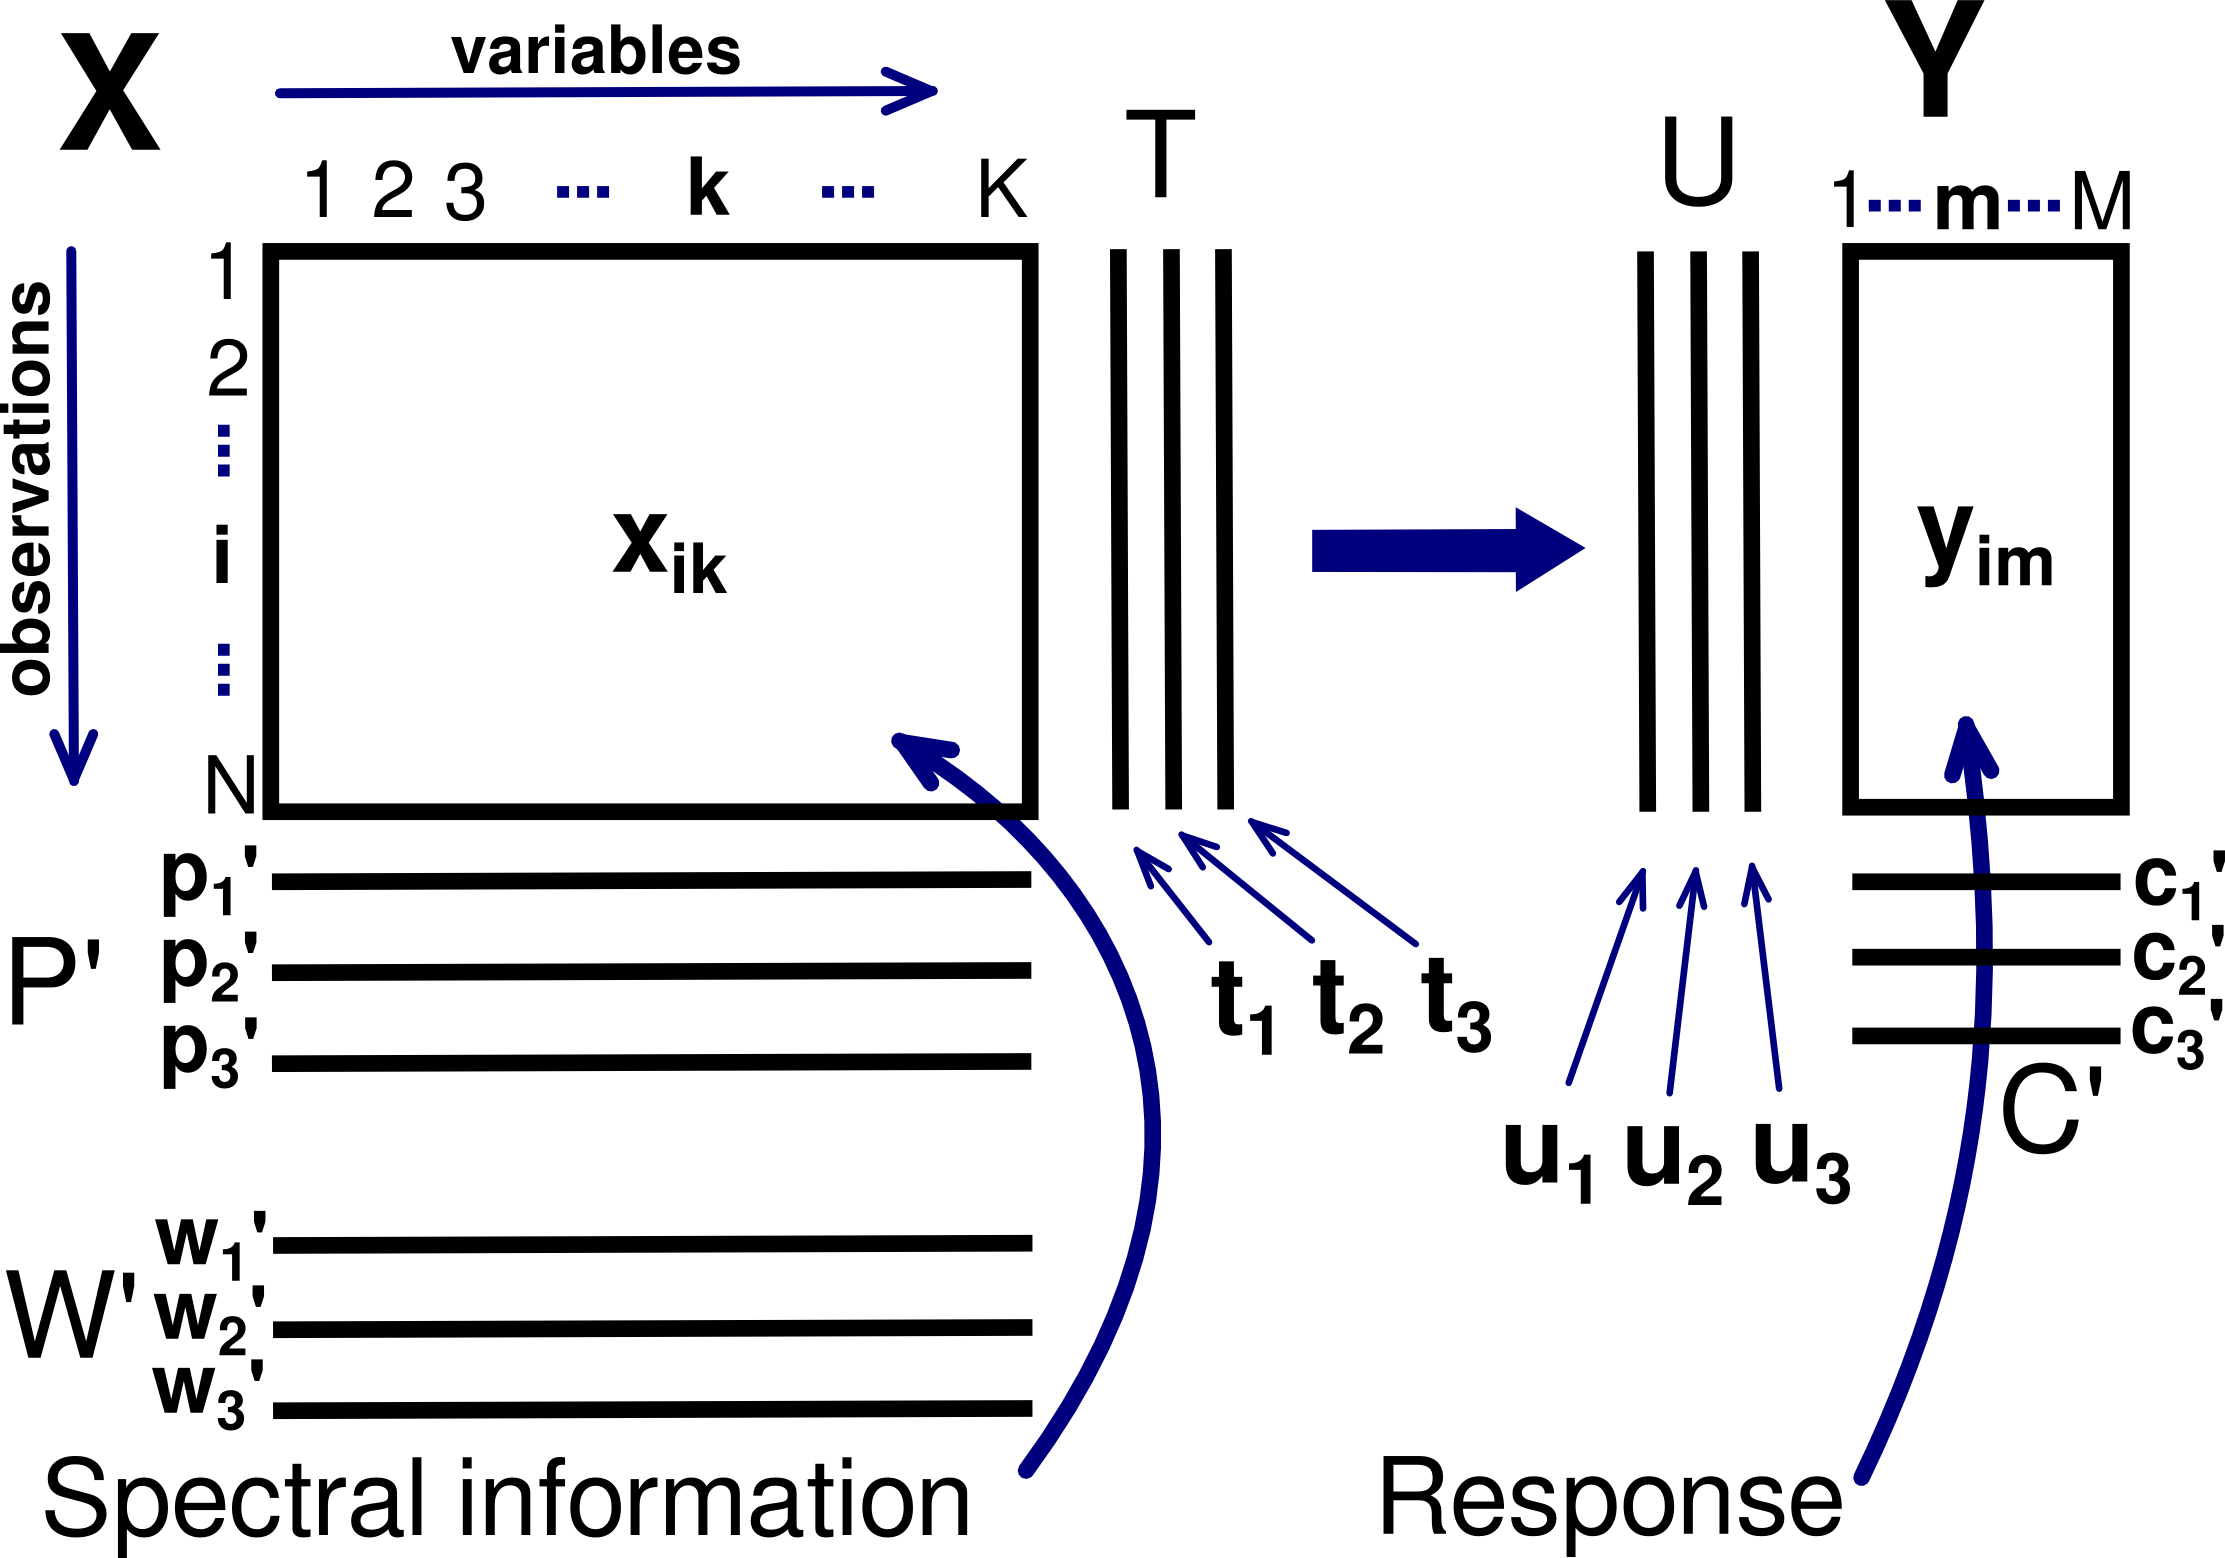
\includegraphics[width=4in]{figs/mva/01-bilinear.png}
\end{center}
\caption
      [Canonical Example of a Bilinear Modeling Problem.]{
  {\bf Canonical Example of a Bilinear Modeling Problem.}
  \\
  Illustration of a data matrix $\mathbf{X}$ and a response matrix
  $\mathbf{Y}$, as they are typically used in partial least squares
  modeling problems. In metabolomics applications, the data matrix will
  contain a set of $N$ spectra, each having $K$ variables. For supervised
  modeling problems, each observation in the data matrix is paired with a
  corresponding row in the response matrix that holds either continuously
  varying outputs or binary class memberships. The data are then decomposed
  into a small number of score vectors ($\mathbf{t}$) and loading vectors
  ($\mathbf{p}$), with corresponding weight vectors ($\mathbf{w}$) used
  to transform the observations in $\mathbf{X}$ into scores-space. The
  responses in $\mathbf{Y}$ are similarly decomposed into scores
  ($\mathbf{u}$) and loadings ($\mathbf{c}$). Tick marks denote
  transposition.
}
\end{figure}

\section{Multivariate Datasets}

\begin{doublespace}
In the majority of cases, multivariate datasets used in metabolomics take the
form of second-order tensors in $\mathbb{R}^{N \times K}$. More simply, these
datasets are real matrices having $N$ rows and $K$ columns. By convention,
the data are arranged as $N$ observation row vectors of length $K$, where $K$
is referred to as the dimensionality of the dataset (Figure 3.1). Typical
examples of 1D datasets include sets of \hnmr{} or \cnmr{} NMR spectra
\cite{beckonert:nprot2007,koh:colon2009}, direct-injection mass spectra
(DI-MS, \cite{castrillo:phch2003,southam:anchem2007,zhou:asms2010}), infrared
(IR) and Raman spectra \cite{ellis:analyst2006,cherney:anchem2007}, or
capillary electrophoretograms (CE, \cite{ramautar:trac2006}). This remarkable
diversity of instrumental platforms used in metabolomics is traceable to the
ability of bilinear factorizations such as principal component analysis
(PCA, \cite{jolliffe2002}) and partial least squares (PLS, \cite{wold1993}) to
directly accept these second-order tensors for modeling (vide infra).
\\\\
The dimensionality of a multivariate dataset may be increased by adding another
``mode'', resulting in a third-order (or higher) tensor
($\mathbf{X} \in \mathbb{R}^{N \times K_1 \times K_2}$, Figure 3.2). In such
cases, the total dimensionality of the dataset is now the product of the
dimensionalities along each mode of the data tensor (e.g. $K_1 \times K_2$).
Third-order tensors are the natural data structures for sets of two-dimensional
observations, including \hhnmr{}, \hcnmr{} and \hnnmr{} NMR spectra, hyphenated
chromatography-mass spectra (LC-MS, GC-MS), hyphenated electrophoresis-mass
spectra (CE-MS), and hyphenated ion-mobility mass spectra (IM-MS). While
third-order data tensors may hold substantially more chemical information than
their second-order counterparts, they are not directly compatible with bilinear
factorization methods, and they require specialized processing,
treatment and modeling algorithms \cite{lu:ieee2009,lu:pr2011}. As an example,
tensors may be vectorized into matrices \cite{hedenstrom:cils2008} that are
suited for PCA and PLS, but at the cost of lost structural information. Methods
such as uncorrelated multilinear PCA (UMPCA, \cite{lu:ieee2009}), on the other
hand, provide a means of directly decomposing tensors into low-dimensional
spaces while maintaining structural information.
\end{doublespace}

\begin{SCfigure}
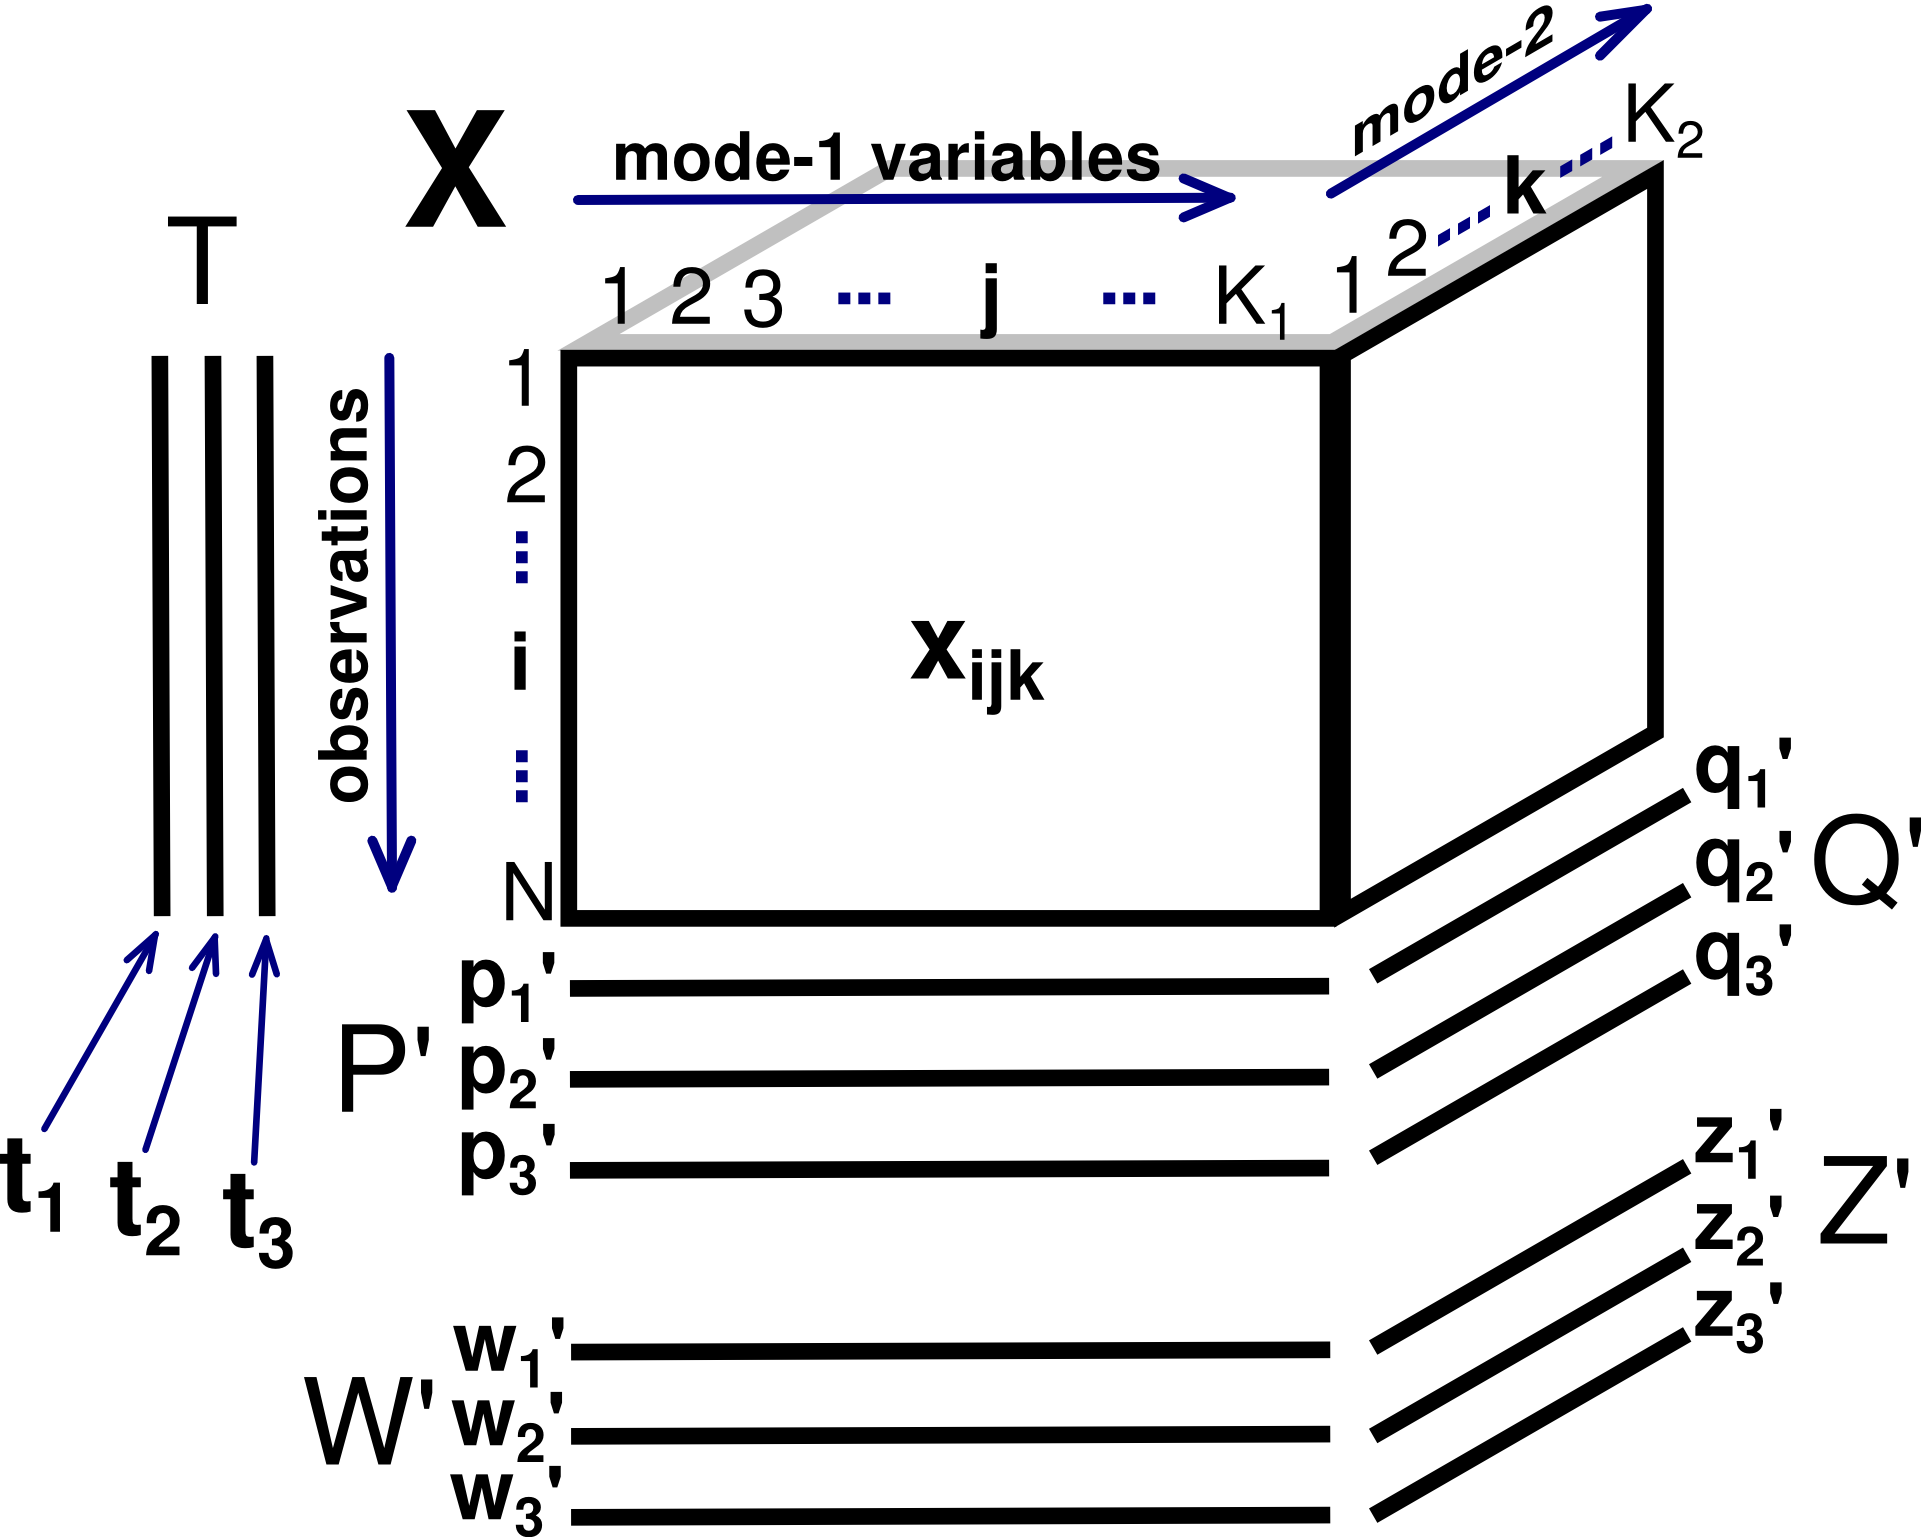
\includegraphics[width=3.5in]{figs/mva/02-trilinear.png}
\caption
      [Canonical Example of an Unsupervised Trilinear Modeling Problem.]{
  {\bf Canonical Example of an Unsupervised Trilinear Modeling Problem.}
  \\
  Illustration of a third-order data tensor $\mathbf{X}$ as may be found in
  multilinear factorization problems. Such data tensors will contain a set
  of $N$ spectra, each having $K_1$ variables along their first mode and
  $K_2$ variables along their second. The data tensor is then decomposed
  into a small number of score vectors ($\mathbf{t}$) and loading vectors
  ($\mathbf{p}$, $\mathbf{q}$), with corresponding weight vectors
  ($\mathbf{w}$, $\mathbf{z}$) used to transform the observations in
  $\mathbf{X}$ into scores-space. Tick marks denote transposition.
}
\end{SCfigure}

\begin{figure}[hb!]
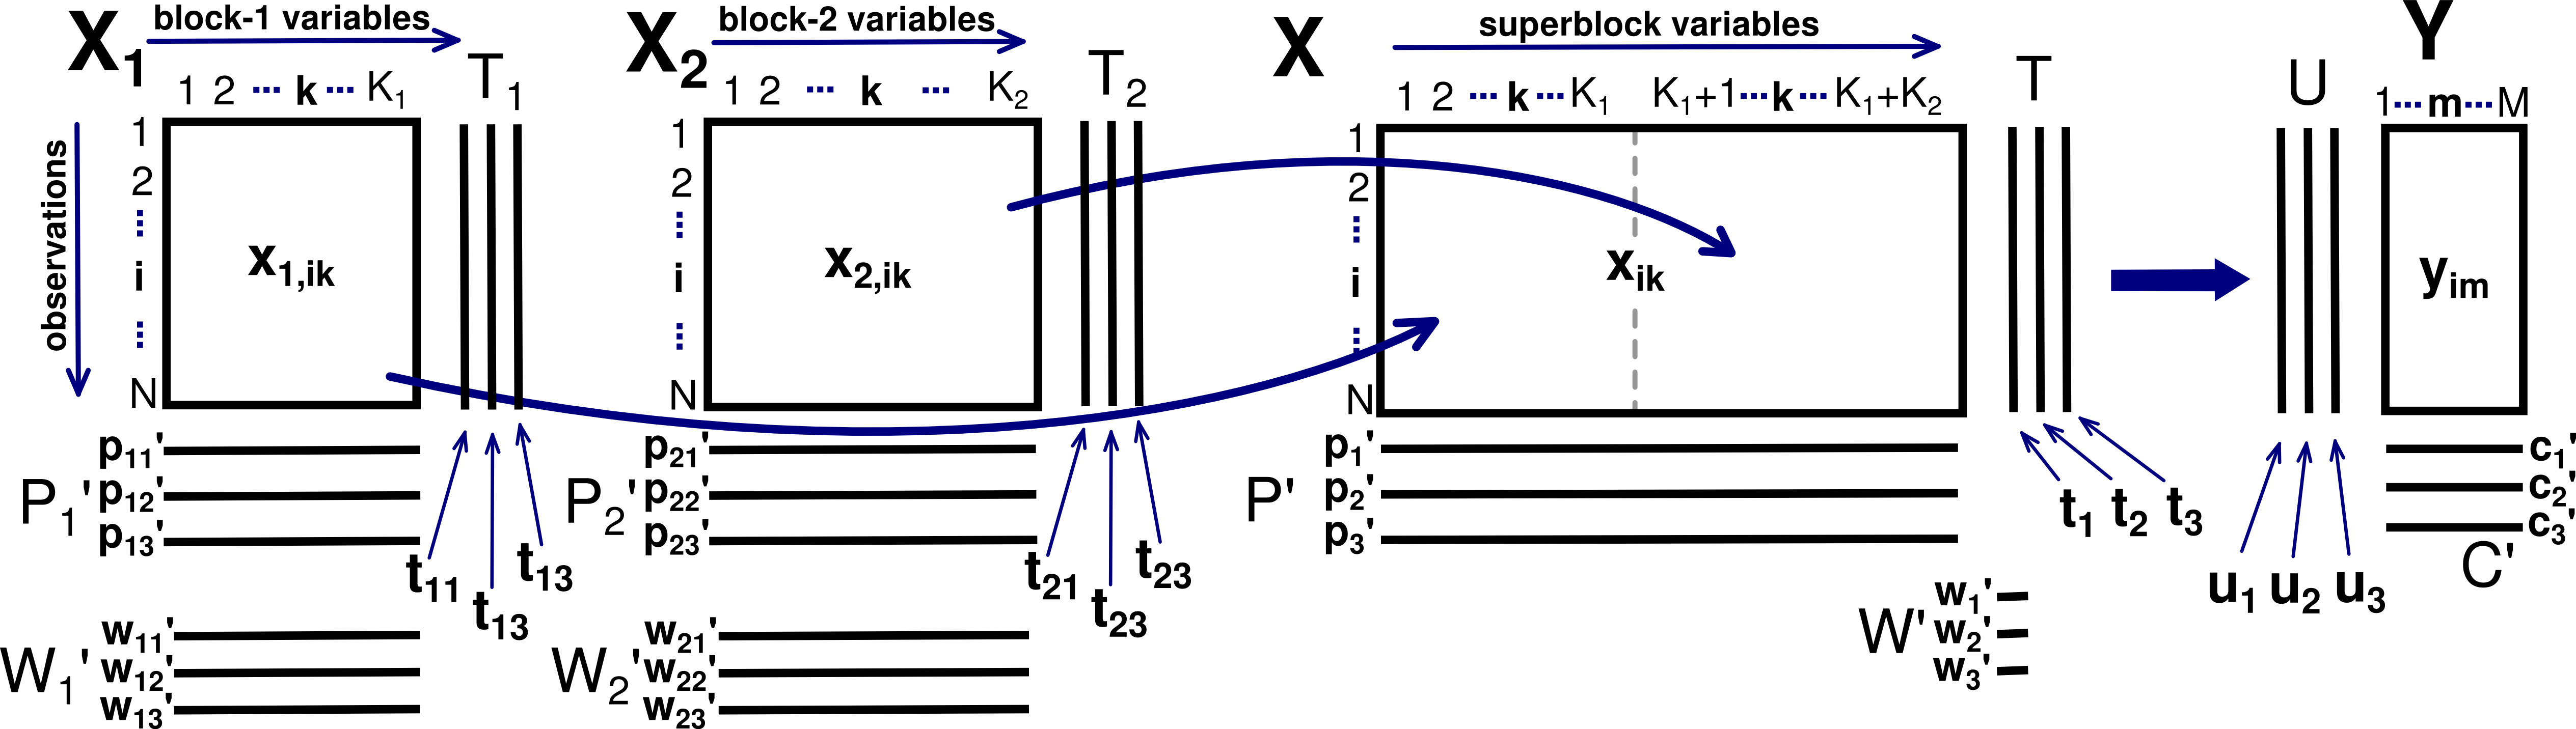
\includegraphics[width=6.5in]{figs/mva/03-multiblock.png}
\caption
      [Canonical Example of a Multiblock Bilinear Modeling Problem.]{
  {\bf Canonical Example of a Multiblock Bilinear Modeling Problem.}
  \\
  Illustration of a pair of data matrices $\mathbf{X}_1$ and $\mathbf{X}_2$,
  their observation-wise concatenation $\mathbf{X}$, and a response matrix
  $\mathbf{Y}$, as they are typically used in multiblock partial least squares
  modeling problems. In metabolomics applications, each data matrix
  $\mathbf{X}_b$ in the set of $B$ matrices will contain a set of $N$ spectra,
  each having $K_b$ variables. The data are then decomposed into a small number
  of superblock score vectors ($\mathbf{t}$) and superblock loading vectors
  ($\mathbf{p}$), with corresponding superblock weight vectors ($\mathbf{w}$).
  Each individual data matrix is also decomposed into a set of block scores
  ($\mathbf{t}_b$), block loadings ($\mathbf{p}_b$) and block weights
  ($\mathbf{w}_b$). Tick marks denote transposition.
}
\end{figure}

\begin{doublespace}
Another mechanism of increasing the information content of datasets entering
into multivariate chemometric models is to collect spectral observations on
two or more complementary instrumental platforms for each sample. In such a
``multiblock'' modeling approach, each data block $\mathbf{X}_b$ contains $N$
$K_b$-variate observations \cite{westerhuis:jchemo1998,smilde:jchemo2003}.
Bilinear methods such as consensus PCA (CPCA), hierarchical PCA and PLS, and
multiblock PLS may then be used to provide information about data variation
that is correlated between data blocks. Recent examples of multiblock modeling
in metabolomics include fusions of near-IR and mid-IR spectra
\cite{bras:cils2005}, \hnmr{} NMR and direct injection electrospray mass
spectra (DI-ESI-MS, \cite{marshall:metab2015}), and observations from multiple
sensors in process control applications \cite{ferreira:jchemo2010}.
\end{doublespace}

\section{Spectral Processing}

\begin{doublespace}
Following the acquisition of experimental data, instrumentation-specific
processing must be applied to transform the data into a suitable set of
real matrices for bilinear modeling, or tensors for multilinear modeling.
Because the majority of data presented herein originated from an NMR
spectrometer, and because NMR spectra present unique challenges to the
analyst during data handling, the following discussions will center around
processing of 1D and 2D NMR datasets.
\end{doublespace}

\subsection{NMR Signals}

\begin{doublespace}
Modern NMR spectrometers effectively acquire a rotating-frame free induction
decay (FID) through the use of quadrature phase detection of the incoming
signal \cite{levitt2008}. This detection method imparts relative phase
information to the time-domain decays by creating an ``in-phase'' signal
component $i(t)$ and a ``quadrature'' component $q(t)$ phased ninety degrees
from $i(t)$. Indirect dimensions of multidimensional NMR experiments are also
collected in quadrature through interleaved acquisition of one-dimensional
decays that have been cosine- and sine-modulated by the indirect-dimension
signals \cite{states:jmr1982}. As a result, each data point in a
$D$-dimensional NMR signal collected in complete quadrature exists in a
hypercomplex space $\mathbb{H}_D$ \cite{schuyler:jmr2013}, which is defined by
a real basis element and $D$ complex basis elements:
\begin{equation}
\Phi_D \equiv \{ 1 \cdot u_1 \cdots u_D \}
\end{equation}
where multiplication by any complex element $u_d$ results in a ninety degree
phase shift in dimension $d$, and the basis elements combine commutatively
under multiplication, as follows:
\begin{align}
u_i u_j =& u_j u_i \\
u_i^2 =& -1
\end{align}

The basis elements in $\Phi_D$ are a generating set for the complete set of
components of the hypercomplex space $\mathbb{H}_D$. For example, in three
dimensions:
\begin{equation}
\Phi_3 = \{ 1, u_1, u_2, u_1 u_2, u_3, u_1 u_3, u_2 u_3, u_1 u_2 u_3 \}
\end{equation}

A scalar in $\mathbb{H}_D$ is then expressed as a linear combination of this
component set. For the three-dimensional example:
\begin{equation}
x = a + b u_1 + c u_2 + d u_1 u_2
  + e u_3 + f u_1 u_3 + g u_2 u_3 + h u_1 u_2 u_3
\end{equation}
or, more generally and succinctly:
\begin{equation}
x = \sum_{\phi \in \Phi_D} x \{ \phi \} \cdot \phi
\end{equation}
where $x\{\phi\}$ denotes the real coefficient of $x$ that scales the basis
component $\phi$ in $x$. For the above three-dimensional example, the
expression $x\{u_1 u_3\}$ would evaluate to $f$. Finally, the expression of
hypercomplex tensors is formally accomplished by defining each coefficient
as a real tensor of appropriate size, like so:
\begin{equation}
x \{ \phi \} \in \mathbb{R}^{k_1 \cdots k_K} \quad \forall \phi \in \Phi_D
\end{equation}
where $K$ is the number of modes of the tensor. The above equation may be
compactly written as $\mathbb{H}_D^{k_1 \cdots k_K}$. Any scalar
in $\mathbb{H}_D$ -- and therefore any data point in a $D$-dimensional
quadrature-complete NMR dataset -- shall require $2^D$ real coefficients
in order to be completely determined. While the hypercomplex
algebras $\mathbb{H}_0$ and $\mathbb{H}_1$ are isomorphic to the real 
($\mathbb{R}$) and complex ($\mathbb{C}$) numbers, respectively, $\mathbb{H}_2$
and $\mathbb{H}_3$ are {\it not} isomorphic to the quaternions and octonions,
as the latter are noncommutative under multiplication. This hypercomplex
algebra, introduced for partial-component nonuniform subsampling by Schuyler
et al. \cite{schuyler:jmr2013}, provides an elegant formalism for expressing
and handling NMR data.
\\\\
Mathematically, 1D NMR free induction decays are described by the following
commonly used parametric signal model:
\begin{equation}
f(t) = \sum_{m=1}^M \alpha_m \exp\left\{
  u_1 (\omega_m t + \theta_m) - \rho_m t
  \right\}
\end{equation}
where $\alpha_m$, $\omega_m$, $\theta_m$ and $\rho_m$ represent the amplitude,
frequency, phase error and decay rate of the $m$-th damped complex exponential
in the model $f(t)$. Using the above formalism for hypercomplex tensors, this
signal model is trivially extended to any number of dimensions by multiplying
in a modulation term for each dimension:
\begin{equation}
f(\mathbf{t}) = \sum_{m=1}^M \alpha_m \prod_{d=1}^D \exp\left\{
  u_d (\omega_{m,d} t_d + \theta_{m,d}) - \rho_{m,d} t_d
  \right\}
\end{equation}

For example, a 2D FID may be modeled as follows:
\begin{equation}
f(t_1, t_2) = \sum_{m=1}^M \alpha_m \exp\left\{
  u_1 (\omega_{m,1} t_1 + \theta_{m,1}) +
  u_2 (\omega_{m,1} t_2 + \theta_{m,2}) -
  \rho_{m,1} t_1 - \rho_{m,2} t_2
  \right\}
\end{equation}

In short, NMR free induction decays may be treated as sums of damped
hypercomplex exponentials. While it is possible to directly parameterize
$f(\mathbf{t})$ using either maximum likelihood estimation
\cite{chylla:jbnmr1995,chylla:jbnmr1998,chylla:anchem2011} or Bayesian
model selection and estimation
\cite{bretthorst:jmr1990a,
      bretthorst:jmr1990b,
      bretthorst:jmr1990c,
      chylla:jbnmr1993}, this chapter will focus on the soft modeling of
multiple NMR spectra using bilinear matrix factorizations. However, the above
parametric description of NMR data is useful in understanding various
processing tasks required by these hypercomplex tensors.
\end{doublespace}

\subsection{Time-domain Processing}

\begin{doublespace}
Processing of acquired NMR data is broken into two stages, where time-domain
data is manipulated, transformed into the frequency domain, and further
processed using frequency-domain functions \cite{hoch1996}.
The most routinely used time-domain NMR processing function -- and the first
to be applied during processing -- is referred to as apodization, where the
free induction decay tensor is multiplied point-wise by a window function
$w(\mathbf{t})$ that varies over $\mathbf{t}$. Multiplication by this window
function serves several purposes, including noise reduction, resolution
enhancement, shaping of individual resonances and removal of $\sin(x)/x$
truncation artifacts in the frequency domain. During apodization, it is also
common practice to selectively scale the first collected data point in an
attempt to reduce later frequency-domain baseline distortions
\cite{stoch:jmr2005,ebel:jmr2006}.
\\\\
Following apodization, one or more dimensions of the time-domain NMR data may
be extended with zeros, a process known as zero-filling. Doubling of the number
of data points by zero-filling is a well-established method of increasing both
the digital resolution and the signal-to-noise ratio (SNR) of an NMR signal,
and further zero-filling only achieves a smoother interpolation of signals in
the frequency domain \cite{ebel:jmr2006}. A final use of zero-filling is to
augment the size of a given dimension into a power of two, enabling the use of
a fast Fourier transform (FFT, \cite{cooley:mcomp1965}) in lieu of the slower
discrete Fourier transform (DFT) to move the data into the frequency domain.
\end{doublespace}

\begin{figure}[ht!]
\includegraphics[width=6.5in]{figs/mva/04-windows.png}
\caption
      [Commonly Applied Window Functions.]{
  {\bf Commonly Applied Window Functions.}
  \\
  Window functions ({\bf A}) produced from a 3.0 Hz exponential (red), a
  3.0 Hz Gaussian (green), and a squared-cosine (blue). Discrete Fourier
  transforms of the window functions in ({\bf A}), zoomed around the first
  few (low frequency) data points, are shown in ({\bf B}). Multiplication of
  a time-domain signal by a given window function in ({\bf A}) results in a
  convolution of its frequency-domain counterpart with the impulse response
  in ({\bf B}). Frequency values in ({\bf B}) are normalized.
}
\end{figure}

\subsection{Frequency-domain Processing}

\begin{doublespace}
When NMR free induction decays have been digitized on a grid of uniformly
spaced time-domain points, the most convenient method of transforming them
into the frequency domain is the discrete Fourier transform (DFT,
\cite{bretthorst:cmr2008,schuyler:jmr2013}). Using the introduced formalism for
hypercomplex NMR data, the DFT along dimension $d$ of a time-domain vector
$\mathbf{f} \in \mathbb{H}_D^N$ is defined\footnote{
  For succinctness, the set of integers from $\alpha$ to $\beta$
  shall be denoted as $\mathbb{Z}_\alpha^\beta$, i.e.
  $\mathbb{Z}_\alpha^\beta \equiv \{
   i \mid i \in \mathbb{Z} \wedge \alpha \le i \le \beta
   \}$
} as:
\begin{equation}
\mathbf{s}_k = \frac{1}{\sqrt{N}} \sum_{n=0}^{N-1}
  \exp\left\{ -2 \pi u_d \frac{n k}{N} \right\}
  \mathbf{f}_n
  \quad \forall k \in \ints{0}{N-1}
\end{equation}
which is a linear transformation
$\mathcal{F}_d : \mathbb{H}_D^N \to \mathbb{H}_D^N$. Discrete Fourier
transformation of multidimensional NMR data along one dimension requires the
application of $\mathcal{F}_d$ to every $d$-mode vector of the hypercomplex
tensor, and full Fourier transformation requires such an operation along each
mode of the tensor. Discrete Fourier transformation is computationally
efficient when using the FFT, and requires no prior knowledge about the
frequency content of the data. However, when only a subset of data points
have been collected from a uniform Nyquist grid, as is the case during
nonuniform sampling (NUS), the DFT is a sub-optimal estimator of frequency
content, and other non-Fourier methods of transformation are required
\cite{bretthorst:cmr2008,mobli:pnmrs2014}.
\\\\
Once transformed into the frequency domain, NMR spectra require a phase
correction processing step, in which a phase factor $\Theta(\omega)$ is
multiplied point-wise with the data to correct for phase errors
(i.e. $\theta_{m,d}$ terms in $f(\mathbf{t})$) in the data. For example, a
1D phase-factor along dimension $d$ would have the following form:
\begin{equation}
\Theta(\omega) = e^{ -u_d \theta(\omega) }
\end{equation}

Ideally, the detected time-domain free induction decays would arrive in-phase
with respect to the receiver, and fine tuning of acquisition parameters can
often accomplish this \cite{chylla:jbnmr1998}.
However, variations in receiver phase, dead time
between the transmit and receive gating circuits, and delays arising from
analog and digital filtering can all introduce phase errors. These phase
errors mix the in-phase and quadrature components of the hypercomplex signal,
and produce a mixture of desirable absorptive spectral lines and broad
dispersive lines between the real and imaginary components of each data point.
Unmixing of these absorptive and dispersive contributions to the real spectral
component involves the identification of the phase error $\theta(\omega)$, an
expansion of phase error terms as powers of $\omega$:
\begin{equation}
\theta(\omega) = \theta_0 + \theta_1 \omega + \theta_2 \omega^2 + \dots
\end{equation}

Realistically, phase errors higher than first-order are not observed in modern
NMR spectra, and phase correction rests on the determination of a zero-order
phase error ($\theta_0$) and a first-order phase error ($\theta_1$) in each
dimension. This determination may be performed manually, through
software-interactive adjustment of zero- and first-order corrections by the
analyst. However, manual phase correction is generally too time-consuming in
the case of chemometric studies, where there are tens to hundreds of spectra
to correct. In that case, the task of phase correction is handed to any number
of automated routines that correct each spectrum individually. Spectra may be
automatically phase-corrected by maximization of the most negative absorptive
data point \cite{siegel:aca1981}, analysis of the absorption-versus-dispersion
\cite{craig:jmr1988} or symmetry \cite{heuer:jmr1991} characteristics of
spectral lines, baseline optimization \cite{brown:jmr1989} or entropy
minimization \cite{chen:jmr2002}, to name a few. It is important to note that,
when the ultimate fate of the spectral data is multivariate analysis, the
phase-correction of each spectrum in isolation is wasteful of information that
is available from treating the dataset as an ensemble \cite{worley:cils2014},
as phase differences {\it between} spectra non-linearly affect both line shapes
and baseline, possibly emphasizing spectral details that contain no
chemically or biochemically relevant information.
\end{doublespace}

\section{Statistical Treatment}

\begin{doublespace}
The properties of the bilinear factorizations commonly applied in metabolomics
dictate that processed data tensors be treated by one or more operations before
they are suitable for modeling. These statistical treatments generally aim to
either reduce the dimensionality of the data tensor (i.e. binning and variable
selection) or increase the self-consistency of observations and variables
(i.e. alignment, normalization and scaling). Treatment operations are usually
instrumentation-agnostic, as the data at this stage of handling almost always
fall into one of the general structures outlined in
\hyperlink{section.3.2}{Section 3.2}.
\end{doublespace}

\begin{figure}[ht!]
\includegraphics[width=6.5in]{figs/mva/05-binning.png}
\caption
      [Example Bin Region Selection Results.]{
  {\bf Example Bin Region Selection Results.}
  \\
  Simulated \hnmr{} NMR spectra of citrate in 20 samples having pH values
  normally distributed around $6.0 \pm 0.05$ pH units, binned using uniform
  ({\bf A}, {\bf B}), optimized ({\bf C}, {\bf D}) and adaptive-intelligent
  ({\bf E}, {\bf F}) algorithms. Results of bin region integration are shown
  in the bottom panels.
}
\end{figure}

\subsection{Binning}

\begin{doublespace}
Because the chemical shifts of \hnmr{} nuclei depend strongly on temperature,
pH, ionic strength, and several other factors that affect their electronic
environment, spectral datasets acquired for NMR metabolic fingerprinting
suffer from imprecision in \hnmr{} chemical shifts between observations.
This chemical shift imprecision, known as a problem of imperfect correspondence
among variables in $\mathbf{X}$ \cite{aberg:abc2009}, decreases the reliability
and interpretability of multivariate bilinear models (e.g. PCA, PLS) trained
directly on full-resolution spectral data in $\mathbf{X}$. Similar errors in
correspondence may also occur in chromatographic datasets, where small drifts
in retention time arise from instrumental instability, analyte interactions,
and fluctuations in mobile phase and stationary phase composition
\cite{nielsen:jchrom1998}. The traditional method of mitigating imperfect
variable correspondence in a data matrix is to partition the original set
of variables into a smaller set of regions, referred to as bins, and
to integrate each bin to yield a data matrix having reduced dimensionality.
\\\\
While binning masks variable mis-correspondence, filters incoherent
instrumental noise, and achieves substantial dimensionality reduction, it often
hides potentially significant variation in low-intensity resonances nearby
strong signals. If bin regions are specified with a uniform size, binning is
nearly guaranteed to split signals or spectral features into multiple bins,
resulting in undesirable multicollinearities within the reduced variable set.
Optimized binning \cite{sousa:cils2013} attempts to avoid dividing signals
between bins by adjusting uniform bin boundaries into local minima of the
data matrix mean, $\langle\mathbf{X}\rangle$. However, because optimized
binning begins with a uniform bin set, its practical ability to minimize peak
splitting is limited. More complex methods of region identification use either
peak detection \cite{davis:cils2007} or recursive subdivision
\cite{demeyer:anchem2008} in order to define a more optimal bin set without
relying on uniform bin boundaries.
\end{doublespace}

\begin{figure}[hb!]
\includegraphics[width=6.5in]{figs/mva/06-align.png}
\caption
      [Example \emph{i}COshift Alignment Results.]{
  {\bf Example \emph{i}COshift Alignment Results.}
  \\
  Full-resolution ({\bf A}) and interval correlation-optimized shifting
  ({\it i}COshift) aligned ({\bf B}) 1D \hnmr{} NMR spectra from a chemometric
  study of brewed coffee roasts. Spectral alignment was performed such that
  each observation was shifted to maximize correlation with its respective
  group mean. Spectral color indicates the observation index.
}
\end{figure}

\subsection{Alignment}

\begin{doublespace}
Binning capably masks variability in signal positions and provides an effective
means of dimensionality reduction, but it also results in a drastic loss of
fine spectral information, as nearby distinct spectral features have been
integrated together in the binning process. When full spectral resolution is
required during model training and interpretation, the correspondence problem
in NMR and chromatographic datasets may be alternatively addressed by signal
alignment methods. The most commonly applied alignment algorithms rely on
either a warping transformation
\cite{nielsen:jchrom1998,
      forshed:aca2003,
      wu:jcim2006} or linear shifts
\cite{veselkov:anchem2009,
      savorani:jmr2010,
      tomasi:jchrom2011} to bring individual variables of each observation
into alignment with a reference observation, which is usually the mean of
the data. Warping during alignment is more applicable in situations where
a linear dependence between variable index (e.g. retention time) and peak
width is expected. In contrast, shift-based alignment preserves peak width,
which is ideal for spectroscopic datasets. Like binning, all alignment
algorithms must first subdivide the variable set into regions that are then
individually warped or shifted, and considerations similar to those in
binning apply equally well during alignment region selection.
\end{doublespace}

\subsection{Normalization}

\begin{doublespace}
Despite the quantitative nature of most spectroscopic platforms, chemometric
samples exhibit variable total analyte concentrations due to variations in
sample preparation, instrument stability, or even the samples themselves.
These ``dilution errors'' are especially common in metabolomics experiments
using samples of biofluids such as urine, where total concentrations may vary
several orders of magnitude. To ensure spectral intensities in a data tensor
are directly comparable across each observation, normalization is applied to
the tensor \cite{worley:cmb2013}. The most common normalization method used in
chemometrics is unit-integral or constant-sum (CS) normalization, where each
observation is scaled such that its total integral is unity
\cite{craig:anchem2006}. CS normalization does more harm that good, however,
as it introduces false correlations between variables and poorly tolerates
large disparities in intensities between each observation.
\\\\
In an attempt to overcome the drawbacks of CS normalization, Dieterle et al.
introduced probabilistic quotient (PQ) normalization, in which the median
normalization quotient between all corresponding data points is used as an
estimator of the true dilution factor \cite{dieterle:anchem2006}. Shortly
after, a method of normalization based on intensity histogram matching (HM)
was proposed as an alternative to PQ normalization, taking cues from image
processing algorithms \cite{torgrip:metab2008}. Based on their ability to
more accurately recover true dilution factors, both PQ and HM normalization
were reported to outperform CS normalization on real and simulated \hnmr{}
NMR metabolomics data matrices. Finally, while more commonly applied to
IR spectroscopic data, standard normal variate (SNV) and its mathematical
cousin, multiplicative scatter correction (MSC) are also candidate methods
for normalizing data tensors produced by NMR and other spectroscopic
platforms \cite{fearn:cils2009}.
\end{doublespace}

\begin{SCfigure}
\includegraphics[width=3.5in]{figs/mva/07-scaling.png}
\caption
      [Effects of Scaling Noisy Synthetic Spectra.]{
  {\bf Effects of Scaling Noisy Synthetic Spectra.}
  \\
  ({\bf A}) Set of 40 synthetic spectra containing two Lorentzian signals. The
  first set of signals at 7.0 ppm have normally distributed intensities of
  $20 \pm 0.5$ absolute units, and the second set at 3.0 ppm are divided into
  two sets of intensities, the first normally distributed around $25 \pm 0.5$
  units and the second around $30 \pm 0.5$ units.
  \\
  ({\bf B}) The same set of synthetic spectra after subtraction of the sample
  mean of the data matrix. The two sets of intensities at 3.0 ppm now appear
  markedly different after centering.
  \\
  ({\bf C}) The set of synthetic spectra after unit variance (UV) scaling,
  illustrating the strong noise amplification effect of the UV method.
  \\
  ({\bf D}) The set of synthetic spectra after Pareto scaling, in which noise
  amplification is reduced relative to UV scaling.
}
\end{SCfigure}

\subsection{Scaling}

\begin{doublespace}
Because bilinear factorization methods such as PCA and PLS generate models
based on the eigenstructure of the covariance matrices of $\mathbf{X}$ and
$\mathbf{Y}$ (vide infra), they are sensitive to the magnitudes of individual
variables in those matrices. Variables with greater intensity -- and therefore
greater variance -- in a data matrix will draw the attention of these methods,
resulting in an unequal weighting of variable importance during model training
\cite{jolliffe2002,smilde:anchem2005,vandenberg:bmcg2006}. As a consequence,
analysts commonly apply one or more scaling transformations to their data prior
to modeling. The simplest and most pervasive method, referred to as Unit
Variance (UV) scaling, centers each variable with respect to its mean and
scales by its standard deviation, like so:
\begin{equation}
\tilde{x}_{nk} = \frac{x_{nk} - \bar{x}_k}{s_k}
\end{equation}
where $\widetilde{\mathbf{X}}$ is the scaled data matrix, $\bar{x}_k$ is the
sample mean of the $k$-th variable over all $N$ observations, and $s_k$ is the
corresponding sample standard deviation. Subtraction of the sample mean
facilitates the identification of differences between observations, and
scaling by the sample standard deviation equally weights every variable
in $\mathbf{X}$. When data are UV-scaled, methods that normally analyze
covariance eigenstructure will instead rely on {\it scale-invariant}
correlations between variables. Although UV scaling achieves an equal weighting
of all variables entering into PCA or PLS, it amplifies the weight of noise
variables relative to that of signal variables, resulting in decreased model
utility and reliability \cite{hoefsloot:jchemo2006}. Pareto scaling applies a
less aggressive scaling than UV by retaining partial covariance between
variables in an attempt to reduce this noise amplification:
\begin{equation}
\tilde{x}_{nk} = \frac{x_{nk} - \bar{x}_k}{\sqrt{s_k}}
\end{equation}

A more advanced scaling method that avoids noise amplification uses a maximum
likelihood scaling transformation (MALS, \cite{hoefsloot:jchemo2006}) that
accounts for the estimated distribution of noise in $\mathbf{X}$. Other forms
of scaling have been developed that emphasize various desirable features in
a data structure. For example, {\it va}riable {\it st}ability (VAST) scaling
multiplies each element by the coefficient of variation of its variable in
order to focus on highly stable spectral features:
\begin{equation}
\tilde{x}_{nk}
 = \frac{x_{nk} - \bar{x}_k}{s_k} \cdot
   \frac{\bar{x}_k}{s_k}
\end{equation}

The alternative level scaling method scales data elements by their sample mean,
effectively focusing later analyses on changes in relative magnitude:
\begin{equation}
\tilde{x}_{nk} = \frac{x_{nk} - \bar{x}_k}{\bar{x}_k}
\end{equation}

However, both VAST and level scaling have a more limited scope of
application than the general UV, Pareto and MALS methods described above, as
they yield optimal transformations only on data structures containing the
features they aim to accentuate. For example, VAST scaling is not suited for
data tensors that contain large variation between experimental groups, unless
further steps are taken to VAST-scale on a (supervised) per-group basis.
\\\\
A special case for scaling occurs during multiblock modeling when two or more
data blocks contain differing variable counts. In these situations, data blocks
having more variables would acquire a larger effective weight during model
training. For example, joint modeling of full-resolution \hnmr{} NMR data
($K \approx 10^3$) and mass spectral data ($K \approx 10^5$) would result in
a weighting of MS variables by a factor of ten relative to NMR variables. To
achieve equal block weighting, the variables of each block must be scaled by
the square root of the number of block variables:
\begin{equation}
\tilde{\tilde{x}}_{bnk} = \frac{\tilde{x}_{bnk}}{\sqrt{K_b}}
\end{equation}
where the second tilde indicates block scaling in addition to any standard
scaling (e.g. UV, Pareto) that may have been applied. When all data blocks
contain analyte concentrations instead of raw spectral variables, range
scaling may be applied prior to block scaling to remove instrumental response
factors and transform all concentrations into relative values
\cite{smilde:anchem2005}:
\begin{equation}
\tilde{x}_{bnk}
 = \frac{x_{bnk} - \bar{x}_{bk}}
        {\max_n(x_{bnk}) - \min_n(x_{bnk})}
\end{equation}

Range scaling holds intuitive appeal for multiblock modeling of concentration
data, but its application to other kinds of datasets is ill-advised, as it
suffers from similar noise amplification problems as UV scaling.
\end{doublespace}

\subsection{Variable Selection}

\begin{doublespace}
Due to the expense of sample preparation and data acquisition in metabolomics
studies, a strong temptation exists to retain all observed variables during
multivariate analyses \cite{kjeldahl:jchemo2010}. Because variables are scaled
to equal (or nearly equal) weight prior to modeling, this practice produces
multivariate models that suffer in both predictive ability and general
reliability. In short, only variables that are truly relevant to the chemical
system under study should be included during modeling. To that end,
conservative manual removal of irrelevant variables based on spectroscopic
and biochemical domain knowledge is often performed in metabolomics. \hnmr{}
NMR datasets, for instance, nearly always contain highly varying signals from
solvents, buffers, and chemical shift reference compounds, all of which may
confound or overshadow relevant sources of variation. Variables containing
such signals, as well as signal-free variables that only contain instrumental
noise, are excellent candidates for manual variable selection. More
computationally intensive methods of variable selection, including support
vector machine recursive feature elimination (SVM-RFE), genetic algorithms
(GA), random forests (RF) and bootstrapping have also been developed to more
aggressively select variables from multivariate data structures
\cite{lin:metab2011,wongravee:anchem2009}. While it is important to retain
only relevant variables for modeling, an over-aggressive variable selection
is equally detrimental, as it leads to over-fit models that may fail to
tolerate subsequent outlying observations.
\end{doublespace}

\section{Modeling}

\begin{doublespace}
The most widely applied modeling methods in metabolomics -- namely principal
component analysis, partial least squares and orthogonal projections to latent
structures (OPLS, \cite{trygg:jchemo2002}) -- fall within a class of methods
known as bilinear matrix factorizations. The general form of a bilinear matrix
factorization is:
\begin{equation}
\mathbf{X} = \mathbf{T} \mathbf{P}^T + \mathbf{E}
\end{equation}
where the data matrix $\mathbf{X} \in \mathbb{R}^{N \times K}$ is approximated
by the product of two matrices, $\mathbf{T} \in \mathbb{R}^{N \times A}$ and
$\mathbf{P} \in \mathbb{R}^{K \times A}$, which are referred to as ``scores''
and ``loadings'', respectively. The matrix
$\mathbf{E} \in \mathbb{R}^{N \times K}$ holds any variation in $\mathbf{X}$
that is not captured by the scores and loadings. To understand how such a
factorization may be used to approximate a data matrix, it is instructive to
consider the product of scores and loadings in vector form:
\begin{equation}
\mathbf{X} = \sum_{a=1}^A \mathbf{t_a} \mathbf{p_a}^T + \mathbf{E}
\end{equation}
where $\mathbf{t_a}$ and $\mathbf{p_a}$ are the $a$-th columns of the score
and loading matrices, respectively. In other words, the data matrix is
approximated by a set of $A$ rank-1 matrices that are constructed by the
outer products of each pair of scores and loadings. Because $A$ is commonly
much less than either $N$ or $K$, these bilinear factorizations are also
referred to as low-rank approximations of their data matrices.
\end{doublespace}

\begin{figure}[ht!]
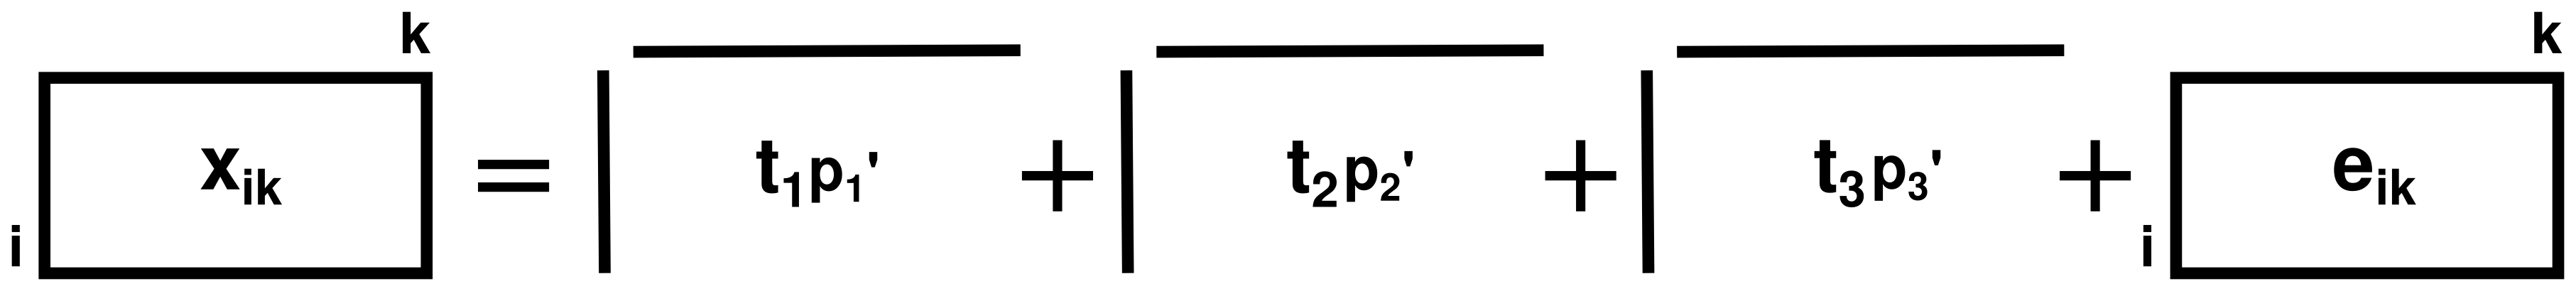
\includegraphics[width=6.5in]{figs/mva/08-lowrank.png}
\caption
      [Example Three-component Bilinear Low-rank Approximation.]{
  {\bf Example Three-component Bilinear Low-rank Approximation.}
  \\
  Depiction of a three-component bilinear low-rank approximation
  $\mathbf{T} \mathbf{P}^T$ of a data matrix $\mathbf{X}$ having
  residuals $\mathbf{E}$, with each outer product of the approximation
  broken out.
}
\end{figure}

\begin{doublespace}
It is important to note that nearly every data matrix modeled by equation
(3.20) in metabolomics contains far fewer observations than variables
(i.e. $N \ll K$) \cite{worley:cmb2013}. In this situation, there are infinitely
many solutions to the equation that yield the same error $\mathbf{E}$. This is
easily demonstrated by multiplying the scores and loadings by an orthonormal
matrix $\mathbf{R} \in \mathbb{R}^{A \times A}$:
\begin{align}
\mathbf{X}
 =& \: \hat{\mathbf{T}} \hat{\mathbf{P}}^T + \mathbf{E}
\nonumber \\
 =& \: \mathbf{T} \mathbf{R} \mathbf{R}^T \mathbf{P}^T + \mathbf{E}
\nonumber \\
 =& \: \mathbf{T} \mathbf{P}^T + \mathbf{E}
\end{align}
where $\hat{\mathbf{T}} = \mathbf{T} \mathbf{R}$ and
$\hat{\mathbf{P}} = \mathbf{P} \mathbf{R}$. A similar expansion of the solution
set may be accomplished by multiplying the scores by a diagonal $A \times A$
matrix, and multiplying the loadings by the inverse of the same diagonal
matrix. This equivalence of an infinite number of solutions to equation
(3.20), known as the problems of rotational and scale ambiguity, is solved by
placing constraints on the values that scores and loadings may take
\cite{dejuan:aca1997,jolliffe2002}. The choice of constraints defines a
particular bilinear factorization method as unique, and determines what
kind of information is sought from a data matrix using that method.
\end{doublespace}

\subsection{Principal Component Analysis}

\begin{doublespace}
In principal component analysis (PCA), which exactly follows equation (3.20),
the loading vectors in $\mathbf{P}$ are constrained to be an orthonormal basis
set. More precisely, the loadings produced by PCA are not just any orthonormal
basis, but are in fact the first $A$ eigenvectors of the sample covariance
matrix $\mathbf{X}^T \mathbf{X}$. In chemometrics, the most commonly used
algorithm for constructing PCA models is nonlinear iterative partial least
squares (NIPALS, \cite{geladi:aca1986}):
\end{doublespace}

\begin{algorithm}[H]
\caption{NIPALS Algorithm for PCA}
\label{algorithm.3.1}
\begin{algorithmic}[1]
\REQUIRE $\mathbf{X} \in \mathbb{R}^{N \times K}$
\ENSURE $\mathbf{t} \in \mathbb{R}^N$, $\mathbf{p} \in \mathbb{R}^K$
\STATE $\mathbf{t}^{(0)} \sim U_{N \times 1}$ \COMMENT{
  $\mathbf{t}$ may also be initialized to a column of $\mathbf{X}$
}
\STATE $k \gets 1$
\REPEAT
  \STATE $\mathbf{p}^{(k)} \propto \mathbf{X}^T \mathbf{t}^{(k-1)}$
  \STATE $\mathbf{t}^{(k)} \gets \mathbf{X} \mathbf{p}^{(k)}$
  \STATE $k \gets k + 1$
\UNTIL{
  $\frac{\| \mathbf{t}^{(k)} - \mathbf{t}^{(k-1)} \|_2}
        {\| \mathbf{t}^{(k-1)} \|_2} < \varepsilon$
}
\end{algorithmic}
\end{algorithm}

\begin{SCfigure}
\includegraphics[width=3.5in]{figs/mva/09-pca.png}
\caption
      [Principal Components of Synthetic Bivariate Data.]{
  {\bf Principal Components of Synthetic Bivariate Data.}
  \\
  ({\bf A}) Set of 100 points drawn from a bivariate normal distribution,
  and the corresponding principal components computed by eigendecomposition
  of the points' sample covariance matrix. Bold and thin arrows indicate the
  normalized and un-normalized loadings, respectively.
  \\
  ({\bf B}) Set of 100 points drawn from two bivariate normal distributions
  having different means, where the major source of variation in the data is
  orthogonal to the direction that separates the two groups.
  \\
  ({\bf C}) Set of 100 points drawn from two bivariate normal distributions
  having different means, where the major source of variation is parallel to
  the direction that separates the groups.
}
\end{SCfigure}

\begin{doublespace}
where $\gets$ indicates assignment, and $\propto$ indicates normalized
assignment. In others words, the following two statements:
\begin{equation*}
a \propto b \quad \Leftrightarrow \quad a \gets \frac{b}{\|b\|_2}
\end{equation*}
are in fact equivalent. In summary, NIPALS PCA initializes a score vector from
a uniform random distribution, and repeatedly projects the rows and columns of
$\mathbf{X}$ into the score and loading vectors until the scores converge to
a predefined limit $\varepsilon$. By substituting the scores assignment into
the loadings assignment, we arrive at the following iteration equation:
\begin{equation}
\mathbf{p}^{(k)} \gets
 \frac
  {\mathbf{X}^T \mathbf{X} \mathbf{p}^{(k-1)}}
  {\| \mathbf{X}^T \mathbf{X} \mathbf{p}^{(k-1)} \|_2}
\end{equation}
which is the equation for power iteration on $\mathbf{X}^T \mathbf{X}$
\cite{golub2012}. Indeed, the NIPALS algorithm implicitly computes the
dominant eigenvector $\mathbf{p}$ of the $K \times K$ sample covariance
matrix, with a corresponding eigenvalue $\mathbf{t}^T \mathbf{t}$. The above
algorithm computes a single principal component of $\mathbf{X}$ in the form
of $\mathbf{t}$ and $\mathbf{p}$. In order to compute a second component,
the first component's contributions must be subtracted from $\mathbf{X}$,
a step referred to as ``deflation'':
\begin{equation}
\mathbf{X}' \gets \mathbf{X} - \mathbf{t} \mathbf{p}^T
\end{equation}

Re-application of the NIPALS algorithm to the deflated matrix $\mathbf{X}'$
will then produce the second principal component of the original data matrix
$\mathbf{X}$. This process of power iteration and deflation is repeated until
an optimal number of components $A^\ast$ is reached.
\end{doublespace}

\subsubsection{PCA for Unsupervised Modeling}

\begin{doublespace}
From the algebraic properties of PCA, an intuitive geometric picture may be
constructed (Figure 3.9). In essence, PCA determines the directions within
a data matrix -- the principal components -- that contain the greatest sources
of variation in that matrix (3.9A), where each direction is constrained
to be orthogonal to all previous directions. When observations in $\mathbf{X}$
fall into two or more experimental groups, they produce different clustering
patterns in the PCA scores $\mathbf{T}$. In cases where the within-group
variation in one or more groups is the major source of variation in
$\mathbf{X}$, PCA will fail to effectively separate the groups in scores space
(3.9B). However, when the between-group variation significantly contributes to
the total variation in $\mathbf{X}$, the groups will be well-separated (3.9C).
Thus, PCA is a powerful method of identifying major trends among variables in
a data matrix, as well as general relationships between observations, and does
not bias its results based on class identity. For a description of methods to
quantify separations between experimental groups in PCA scores space, see
\hyperlink{chapter.7}{Chapter 7}.
\end{doublespace}

\subsubsection{PCA for Outlier Detection}

\begin{doublespace}
During data handling, it is common practice to exclude outlying observations,
when warranted by the analysis, in order to ensure relevant information
extraction. In the univariate case, the sample mean $\bar{x}$ and sample
standard deviation $s$ may be estimated from a data vector $\mathbf{x}$,
which may then be standardized into a set of Mahalanobis distances
$\mathbf{d}$:
\begin{equation}
d_n = \frac{x_n - \bar{x}}{s}
 \quad \forall n \in \ints{1}{N}
\end{equation}

These distances in $\mathbf{d}$ may be transformed into $t$ statistics and
compared to critical values of a $t$-distribution using a run plot in order
to visually detect outliers \cite{chambers1983}. In the multivariate case,
the sample mean vector $\bar{\mathbf{x}} \in \mathbb{R}^K$ and the sample
variance-covariance matrix $\mathbf{S} \in \mathbb{R}^{K \times K}$ of the
data matrix $\mathbf{X} \in \mathbb{R}^{N \times K}$ must first be computed:
\begin{align}
\bar{\mathbf{x}} =& \: N^{-1} \sum_{n=1}^N \mathbf{x}_n \\
\mathbf{S} =& \: (N - 1)^{-1} \mathbf{X}^T \mathbf{X}
\end{align}
where $\mathbf{x}_n$ is the $n$-th observation row vector in $\mathbf{X}$.
The set of squared Mahalanobis distances may then be computed as follows
\cite{demaesschalck:cils2000}:
\begin{equation}
d_n^2 =
 (\mathbf{x}_n - \bar{\mathbf{x}}) \mathbf{S}^{-1}
 (\mathbf{x}_n - \bar{\mathbf{x}})^T
 \quad \forall n \in \ints{1}{N}
\end{equation}

Once again, each squared distance may be compared to a critical value from a
$T^2$-distribution to assess the probability that its corresponding observation
is an outlier. The above procedure fails in practice, because the covariance
matrix is severely rank-deficient, and thus non-invertible (i.e. $N \ll K$).
To ensure a stable inversion of the covariance matrix, the data matrix may be
approximated using PCA (i.e. $\mathbf{X} \approx \mathbf{T} \mathbf{P}^T$),
where the number of principal components is less than the rank of the data
matrix. Using the orthonormality property of PCA loadings, squared Mahalanobis
distances may again be obtained from the PCA scores:
\begin{equation}
d_n^2 =
 \mathbf{t}_n
 \left( \frac{\mathbf{T}^T \mathbf{T}}{N - 1} \right)^{-1}
 \mathbf{t}_n^T
 \quad \forall n \in \ints{1}{N}
\end{equation}
where $\mathbf{t}_n$ is the $n$-th row of the scores matrix $\mathbf{T}$.
Because the matrix $\mathbf{T}^T \mathbf{T}$ is diagonal, it is trivially
inverted and calculation of each $d_n^2$ is greatly simplified. Mahalanobis
distances computed using PCA scores are close approximations of their true
values in the original high-dimensional space \cite{demaesschalck:cils2000},
and provide a means of outlier detection in high-dimensional data
(Figure 3.10). Outliers may be visually identified from scatter plots of PCA
scores (3.10B) or from run plots of their corresponding squared Mahalanobis
distances (3.10C). In both cases, the squared Mahalanobis distance is compared
to the $\chi^2$ distribution at a preselected significance $\alpha$ and $A$
degrees of freedom \cite{hotelling:ams1931,worley:abio2013}.
\end{doublespace}

\begin{SCfigure}
\includegraphics[width=3.5in]{figs/mva/10-outlier.png}
\caption
      [PCA for Outlier Testing.]{
  {\bf PCA for Outlier Testing.}
  \\
  ({\bf A}) Set of 40 spectra, generated identically to those in Figure 3.7,
  with the exception of observation 20, which contains an extra Lorentzian
  signal at 6.8 ppm.
  \\
  ({\bf B}) Principal Component Analysis scores plot of the spectral data,
  showing the 68.3\% ($1\sigma$), 95.5\% ($2\sigma$) and 99.7\% ($3\sigma$)
  confidence regions as dashed, thin and bold ellipses, respectively. Point
  colorings indicate relative squared Mahalanobis distances, ranging from blue
  to red as $d^2$ increases.
  \\
  ({\bf C}) Run plot of squared Mahalanobis distances computed from PCA scores
  of the spectral data, again illustrating the one-, two- and three-$\sigma$
  thresholds for outlier detection. Point colorings indicate relative squared
  Mahalanobis distances.
}
\end{SCfigure}

\subsubsection{PCA for Multiple Linear Regression}

\begin{doublespace}
Often, a data matrix $\mathbf{X} \in \mathbb{R}^{N \times K}$ is used within
the context of a multiple linear regression to determine a set of regression
coefficients $\mathbf{B} \in \mathbb{R}^{K \times M}$ that best recapitulate
a set of responses $\mathbf{Y} \in \mathbb{R}^{N \times M}$ using the data in
$\mathbf{X}$:
\begin{equation}
\mathbf{Y} = \mathbf{X} \mathbf{B} + \mathbf{E}
\end{equation}

In which case the ordinary least squares (OLS) estimator of the regression
coefficients is obtained from inversion of the normal equations
\cite{draper1998}:
\begin{equation}
\hat{\mathbf{B}} = (\mathbf{X}^T \mathbf{X})^{-1} \mathbf{X}^T \mathbf{Y}
\end{equation}

The OLS regression coefficients $\hat{\mathbf{B}}$ minimize the sum of squares
of the residual matrix, $\frosq{\mathbf{E}}$, and are maximum likelihood
estimates of $\mathbf{B}$ when the errors are independent and identically
normally distributed \cite{draper1998}. However, the fact that $N \ll K$ yet
again makes the matrix $\mathbf{X}^T \mathbf{X}$ non-invertible, forcing the
analyst down a different path. By replacing the data matrix with its PCA
approximation in the regression equation:
\begin{equation}
\mathbf{Y} = \mathbf{T} \mathbf{P}^T \mathbf{B} + \mathbf{E}'
\end{equation}
it is possible to obtain OLS estimates of the regression coefficients:
\begin{align}
\hat{\mathbf{B}}'
 =& \: (\mathbf{P} \mathbf{T}^T \mathbf{T} \mathbf{P}^T)^{-1}
       \mathbf{P} \mathbf{T}^T \mathbf{Y}
 \nonumber \\
 =& \: \mathbf{P} (\mathbf{T}^T \mathbf{T})^{-1} \mathbf{T}^T \mathbf{Y}
 \\
 =& \: \mathbf{P} \hat{\mathbf{G}}
\end{align}
where the matrix $\hat{\mathbf{G}} \in \mathbb{R}^{A \times M}$ is the set of
OLS regression coefficient estimates in PCA scores space:
\begin{equation}
\mathbf{Y} = \mathbf{T} \mathbf{G} + \mathbf{E}'
\end{equation}

By computing the least-squares estimates of the regression coefficients in the
low-dimensional PCA scores space and projecting those estimates into the
original high-dimensional space, this technique of principal component
regression (PCR, \cite{jolliffe2002}) sidesteps the curse of dimensionality
during estimation. Furthermore, the variances of PCR-estimated coefficients
$\hat{\mathbf{B}}'$ are lower than those of the original OLS estimates
$\hat{\mathbf{B}}$. The PCR method will fail to obtain useful estimates,
however, when response-correlated information in the data matrix is not
a major source of variation (cf. Figure 3.9B). In such cases, methods such
as PLS must be used instead.
\end{doublespace}

\subsection{Partial Least Squares}

\begin{doublespace}
Partial least squares (PLS) approaches the high-dimensional multiple linear
regression problem introduced in equation (3.30) by approximating both
$\mathbf{X}$ \emph{and} $\mathbf{Y}$ using bilinear factorizations
\cite{wold:cils2001}:
\begin{align}
\mathbf{X} =& \: \mathbf{T} \mathbf{P}^T + \mathbf{E} \\
\mathbf{Y} =& \: \mathbf{U} \mathbf{C}^T + \mathbf{G} \\
           =& \: \mathbf{T} \mathbf{C}^T + \mathbf{F} \nonumber
\end{align}
where the last equality indicates that the $\mathbf{X}$-scores are highly
correlated with the $\mathbf{Y}$-scores, and are therefore good predictors
of $\mathbf{Y}$. The most commonly applied algorithm for PLS is once again
NIPALS-based, and is shown below:
\end{doublespace}

\begin{algorithm}[H]
\caption{NIPALS Algorithm for PLS}
\label{algorithm.3.2}
\begin{algorithmic}[1]
\REQUIRE $\mathbf{X} \in \mathbb{R}^{N \times K}$,%
       $\:\mathbf{Y} \in \mathbb{R}^{N \times M}$
\ENSURE $\mathbf{t} \in \mathbb{R}^N$,%
      $\:\mathbf{p} \in \mathbb{R}^K$,%
      $\:\mathbf{w} \in \mathbb{R}^K$,%
      $\:\mathbf{u} \in \mathbb{R}^N$,%
      $\:\mathbf{c} \in \mathbb{R}^M$
\STATE $\mathbf{u} \sim U_{N \times 1}$ \COMMENT{
  $\mathbf{u}$ may also be initialized to a column of $\mathbf{Y}$
}
\REPEAT
  \STATE $\mathbf{w} \propto \mathbf{X}^T \mathbf{u}$
  \STATE $\mathbf{t} \gets \mathbf{X} \mathbf{w}$
  \STATE $\mathbf{c} \gets \tfrac{\mathbf{Y}^T \mathbf{t}}
                                 {\mathbf{t}^T \mathbf{t}}$
  \STATE $\mathbf{u} \gets \tfrac{\mathbf{Y} \mathbf{c}}
                                 {\mathbf{c}^T \mathbf{c}}$
\UNTIL{$\tau < \varepsilon$}
\STATE $\mathbf{p} \gets \tfrac{\mathbf{X}^T \mathbf{t}}
                               {\mathbf{t}^T \mathbf{t}}$
\end{algorithmic}
\end{algorithm}

\begin{SCfigure}
\includegraphics[width=3.5in]{figs/mva/11-pls.png}
\caption
      [PLS Components of Synthetic Bivariate Data.]{
  {\bf PLS Components of Synthetic Bivariate Data.}
  \\
  ({\bf A}) Set of 100 points drawn from a bivariate normal distribution,
  and the corresponding partial least squares weights computed by
  eigendecomposition of the points' cross-covariances with the response
  vector.
  \\
  ({\bf B}) Set of 100 points drawn from two bivariate normal distributions
  having different means, where the major source of variation in the data is
  orthogonal to the direction that separates the two groups. Note the mixing
  of predictive information between both PLS components.
  \\
  ({\bf C}) Set of 100 points drawn from two bivariate normal distributions
  having different means, where the major source of variation is parallel to
  the direction that separates the groups.
}
\end{SCfigure}

\begin{doublespace}
where $\tau$ equals the score convergence value:
\begin{equation}
\tau = \frac{\| \mathbf{t}^{(k)} - \mathbf{t}^{(k-1)} \|_2}
            {\| \mathbf{t}^{(k-1)} \|_2}
\end{equation}
and iteration superscripts have been dropped for readability. Backtracking the
iteration assignments now produces a different iteration equation:
\begin{equation}
\mathbf{w}^{(k)} \gets \frac{
    \mathbf{X}^T \mathbf{Y} \mathbf{Y}^T \mathbf{X} \mathbf{w}^{(k-1)}
}{
 \| \mathbf{X}^T \mathbf{Y} \mathbf{Y}^T \mathbf{X} \mathbf{w}^{(k-1)} \|_2
}
\end{equation}
which is the equation for power iteration on the cross-covariance matrix
$\mathbf{X}^T \mathbf{Y} \mathbf{Y}^T \mathbf{X}$. The NIPALS PLS algorithm
computes the dominant eigenvector $\mathbf{w}$ of the cross-covariances between
the data and responses (cf. Figure 3.11). As in PCA, computation of subsequent
PLS components is achieved by deflating the data and response matrices:
\begin{align}
\mathbf{X}' \gets \mathbf{X} - \mathbf{t} \mathbf{p}^T \\
\mathbf{Y}' \gets \mathbf{Y} - \mathbf{t} \mathbf{c}^T
\end{align}
and re-applying NIPALS on $\mathbf{X}'$ and $\mathbf{Y}'$. Unlike PCA, the PLS
loadings $\mathbf{P}$ are not orthogonal, and the $\mathbf{X}$-scores are
instead obtained through a linear transformation by a set of non-orthogonal
`weights' $\mathbf{W}^\ast \in \mathbb{R}^{K \times A}$, like so:
\begin{equation}
\mathbf{T} = \mathbf{X} \mathbf{W}^\ast
\end{equation}

This allows PLS to be rewritten into the form of a multiple linear regression
model:
\begin{align}
\mathbf{Y} =& \: \mathbf{X} \mathbf{W}^\ast \mathbf{C}^T + \mathbf{F} \\
           =& \: \mathbf{X} \hat{\mathbf{B}}_{PLS} + \mathbf{F} \nonumber
\end{align}

These weights $\mathbf{W}^\ast$, which directly relate to $\mathbf{X}$, may be
computed from the orthonormal weights $\mathbf{W}$ returned from NIPALS through
the following transformation \cite{manne:cils1987}:
\begin{equation}
\mathbf{W}^\ast = \mathbf{W} (\mathbf{P}^T \mathbf{W})^{-1}
\end{equation}
\end{doublespace}

\begin{SCfigure}
\includegraphics[width=3.5in]{figs/mva/12-orthprj.png}
\caption
      [Orthogonal Projections of Synthetic Bivariate Data.]{
  {\bf Orthogonal Projections of Synthetic Bivariate Data.}
  \\
  ({\bf A}) Projection of the set of points in ({\bf B}) onto their
  response-predictive (PLS) component.
  \\
  ({\bf B}) Set of 100 points and their PLS components from Figure 3.11B.
  \\
  ({\bf C}) Projection of the set of points in ({\bf B}) onto their
  response-orthogonal (OPLS) component.
}
\end{SCfigure}

\subsection{Orthogonal Projections to Latent Structures}

\begin{doublespace}
The PLS modeling framework expresses the data and response matrices as a pair
of low-rank bilinear factorizations, where the data scores $\mathbf{T}$ hold
variation in the data that is $\mathbf{Y}$-predictive, as well as variation
that compensates for the $\mathbf{Y}$-uncorrelated portion of the data. As a
result, PLS models typically require more components than response matrix
columns. In other words, $A^\ast \ge M$ for any PLS model, where the two are
equal if and only if no $\mathbf{Y}$-uncorrelated variation is present in
$\mathbf{X}$. This presence of `compensatory correlations' in PLS scores
confounds interpretation of scores and loadings produced by such
non-parsimonious PLS models.
\\\\
One potential solution proposed to deal with $\mathbf{Y}$-uncorrelated
variation, known as orthogonal signal correction
(OSC, \cite{boulet:cils2012,westerhuis:cils2001}), removes variation in the
data matrix that is not correlated to the responses using an orthogonal
projection that reveals $\mathbf{Y}$-predictive variation:
\begin{align}
\mathbf{X_p}
 =& \: \mathbf{X} - \mathbf{T_o} \mathbf{P_o}^T \\
 =& \: \left(
  \mathbf{I} - \mathbf{T_o}
  (\mathbf{T_o}^T \mathbf{T_o})^{-1}
  \mathbf{T_o}^T \right) \mathbf{X}
\end{align}
where the $\mathbf{Y}$-orthogonal scores
$\mathbf{T_o} \in \mathbb{R}^{N \times A_o}$ and loadings
$\mathbf{P_o} \in \mathbb{R}^{K \times A_o}$ may be estimated using a variety
of algorithms \cite{boulet:cils2012}. However, OSC methods tend to suffer from
problems of overfitting, and PLS models trained on data matrices that have been
filtered by OSC are also at risk of being over-fit \cite{trygg:jchemo2002}. As
an alternative to direct methods of orthogonal signal correction, a modified
NIPALS PLS algorithm -- orthogonal projections to latent structures
(OPLS) -- was proposed. Instead of removing \emph{all}
$\mathbf{Y}$-uncorrelated variation in $\mathbf{X}$ prior to PLS modeling,
OPLS only removes $\mathbf{Y}$-uncorrelated variation that interferes with
predictive PLS components, effectively partitioning the variation in the data
matrix into a set of $A_p$ predictive components and a set of $A_o$ orthogonal
components:
\begin{align}
\mathbf{X} =& \: \mathbf{T} \mathbf{P}^T +
                 \mathbf{T_o} \mathbf{P_o}^T + \mathbf{E} \\
\mathbf{Y} =& \: \mathbf{U} \mathbf{C}^T + \mathbf{G} \\
           =& \: \mathbf{T} \mathbf{C}^T + \mathbf{F} \nonumber
\end{align}

The addition of OSC to NIPALS PLS in the form of OPLS is described in the
following algorithm:
\end{doublespace}

\begin{algorithm}[H]
\caption{NIPALS Algorithm for OPLS}
\label{algorithm.3.3}
\begin{algorithmic}[1]
\REQUIRE $\mathbf{X} \in \mathbb{R}^{N \times K}$,%
       $\:\mathbf{Y} \in \mathbb{R}^{N \times M}$
\ENSURE $\mathbf{t} \in \mathbb{R}^N$,%
      $\:\mathbf{p} \in \mathbb{R}^K$,%
      $\:\mathbf{w} \in \mathbb{R}^K$,%
      $\:\mathbf{T_o} \in \mathbb{R}^{N \times a}$,%
      $\:\mathbf{P_o} \in \mathbb{R}^{K \times a}$,%
      $\:\mathbf{W_o} \in \mathbb{R}^{K \times a}$,%
      $\:\mathbf{u} \in \mathbb{R}^N$,%
      $\:\mathbf{c} \in \mathbb{R}^M$
\FORALL{$m \in \ints{1}{M}$}
  \STATE $\mathbf{v}_m \gets \tfrac{\mathbf{X}^T \mathbf{y}_m}
                                   {\mathbf{y}_m^T \mathbf{y}_m}$
  \STATE $\mathbf{V} \gets [\mathbf{V}, \; \mathbf{v}_m]$
\ENDFOR
\STATE $\mathbf{u} \sim U_{N \times 1}$ \COMMENT{
  $\mathbf{u}$ may also be initialized to a column of $\mathbf{Y}$
}
\STATE done $\gets$ \FALSE
\STATE $\mathbf{E} \gets \mathbf{X}$
\STATE $a \gets 0$
\WHILE{\NOT done}
  \REPEAT
    \STATE $\mathbf{w} \propto \mathbf{E}^T \mathbf{u}$
    \STATE $\mathbf{t} \gets \mathbf{E} \mathbf{w}$
    \STATE $\mathbf{c} \gets \tfrac{\mathbf{Y}^T \mathbf{t}}
                                   {\mathbf{t}^T \mathbf{t}}$
    \STATE $\mathbf{u} \gets \tfrac{\mathbf{Y} \mathbf{c}}
                                   {\mathbf{c}^T \mathbf{c}}$
  \UNTIL{$\tau < \varepsilon$}
  \STATE $\mathbf{p} \gets \tfrac{\mathbf{E}^T \mathbf{t}}
                                 {\mathbf{t}^T \mathbf{t}}$
  \STATE $\mathbf{z} \gets \mathbf{p}$
  \STATE $\mathbf{z} \gets \mathbf{z} -
          \tfrac{\mathbf{v}_m^T \mathbf{z}}
                {\mathbf{v}_m^T \mathbf{v}_m} \mathbf{v}_m
          \quad \forall m \in \{1, 2, \dots M\}$
  \STATE $\mathbf{w_o} \propto \mathbf{z}$
  \STATE $\mathbf{t_o} \gets \mathbf{E} \mathbf{w_o}$
  \STATE $\mathbf{p_o} \gets \tfrac{\mathbf{E}^T \mathbf{t_o}}
                                   {\mathbf{t_o}^T \mathbf{t_o}}$
  \STATE $\lambda \gets \tfrac{\| \mathbf{z} \|_2}{\| \mathbf{p} \|_2}$
  \IF{$\lambda > \lambda_{th}$}
    \STATE $\mathbf{T_o} \gets [\mathbf{T_o}, \; \mathbf{t_o}]$
    \STATE $\mathbf{P_o} \gets [\mathbf{P_o}, \; \mathbf{p_o}]$
    \STATE $\mathbf{W_o} \gets [\mathbf{W_o}, \; \mathbf{w_o}]$
    \STATE $\mathbf{E} \gets \mathbf{E} - \mathbf{t_o} \mathbf{p_o}^T$
    \STATE $a \gets a + 1$
  \ELSE
    \STATE done $\gets$ \TRUE
  \ENDIF
\ENDWHILE
\end{algorithmic}
\end{algorithm}

\begin{doublespace}
where $\tau$ is again the convergence value for $\mathbf{t}$. The above OPLS
algorithm computes one predictive (PLS) component in the vectors $\mathbf{t}$
and $\mathbf{p}$, and $a$ orthogonal components in $\mathbf{T_o}$ and
$\mathbf{P_o}$. While the above algorithm appears considerably more complicated
than those for PCA or PLS, it is essentially a PLS algorithm (lines 10--16)
that has been wrapped in an OSC filter (main `done' loop). At each execution
of the main loop, a single PLS component is computed on the current predictive
data matrix, $\mathbf{E}$. If a new orthogonal component may be obtained from
this PLS component that contains significant variation
(i.e. $\lambda > \lambda_{th}$), it is added to the set of orthogonal
components and subtracted from $\mathbf{X_p}$, from which an updated PLS
component is computed. As in PCA and PLS, computation of subsequent OPLS
component sets is achieved by first deflating the data and response matrices:
\begin{align}
\mathbf{X}' \gets& \: \mathbf{X} -
 \mathbf{t} \mathbf{p}^T -
 \mathbf{T_o} \mathbf{P_o}^T \\
\mathbf{Y}' \gets& \: \mathbf{Y} - \mathbf{t} \mathbf{c}^T
\end{align}
and then re-applying NIPALS on $\mathbf{X}'$ and $\mathbf{Y}'$. Like PLS, the
OPLS equations may also be written in the form of a multiple linear regression:
\begin{equation}
\mathbf{Y} =
 \left( \mathbf{X} - \mathbf{T_o} \mathbf{P_o}^T \right)
 \mathbf{W}^\ast \mathbf{C}^T + \mathbf{F}
\end{equation}

It is important to note that OPLS does not outperform PLS in prediction
\cite{tapp:trac2009}, but merely provides a more easily interpretable,
parsimonious model for the analyst. In fact, predictions made by OPLS
models having $A_p$ predictive components and $A_o$ orthogonal components
are identical to those made by PLS models having $A_p + A_o$ components.
Also, when the data matrix contains no $\mathbf{Y}$-uncorrelated variation,
OPLS and PLS will produce identical models.
\end{doublespace}

\subsubsection{O2PLS}

\begin{doublespace}
While the above NIPALS OPLS algorithm is designed to handle matrix-$\mathbf{Y}$
multivariate regression problems, its creators have championed the O2PLS
\cite{trygg:jchemo2003} method instead of OPLS in such situations. Whereas OPLS
is a unidirectional (i.e. $\mathbf{X} \mapsto \mathbf{Y}$) regression method,
the bidirectional O2PLS method considers neither matrix to be special, and
decomposes each matrix into a `local' or `unique' component and a `joint'
component (i.e. $\mathbf{X} \leftrightarrow \mathbf{Y}$). The O2PLS modeling
framework provides an unsupervised means of analyzing relationships between
two spectral data matrices, where variation exists in each matrix that is
uncorrelated to the other.
\end{doublespace}

\subsection{Consensus PCA}

\begin{doublespace}
In analogy to PCA, which seeks directions of maximum variation (loadings) in a
data matrix, the consensus PCA (CPCA-W,
\cite{westerhuis:jchemo1998,smilde:jchemo2003}) seeks
a set of `consensus' loadings $\mathbf{P}_b$ that contain a maximum amount
of variation in each of the $B$ provided data blocks $\mathbf{X}_b$ while
retaining variation relating each block to the others. In essence, CPCA-W
returns a PCA `super-model' for the matrix of concatenated blocks $\mathbf{X}$
and a PCA block model for each individual block $\mathbf{X}_b$:
\begin{align}
\mathbf{X} =& \: [\mathbf{X}_1, \dots \mathbf{X}_B] \\
           =& \: \mathbf{T} \mathbf{P}^T + \mathbf{E} \\
\mathbf{X}_b =& \: \mathbf{T}_b {\mathbf{P}_b}^T + \mathbf{E}_b
 \quad \forall b \in \ints{1}{B}
\end{align}

The NIPALS algorithm for CPCA-W, shown below, returns a pair of super-scores
$\mathbf{t}$ and super-loadings $\mathbf{p}$ that relate to the matrix of
concatenated blocks, as well as a pair of block scores $\mathbf{t}_b$ and
block loadings $\mathbf{p}_b$ for each of the $B$ provided blocks:
\end{doublespace}

\begin{algorithm}[H]
\caption{NIPALS Algorithm for CPCA-W}
\label{algorithm.3.4}
\begin{algorithmic}[1]
\REQUIRE $\mathbf{X}_b \in \mathbb{R}^{N \times K_b}
          \quad \forall b \in \ints{1}{B}$
\ENSURE $\mathbf{t} \in \mathbb{R}^N$,%
      $\:\mathbf{p} \in \mathbb{R}^K$,%
      $\:\mathbf{w} \in \mathbb{R}^B$,%
      $\:\mathbf{t}_b \in \mathbb{R}^N$,%
      $\:\mathbf{p}_b \in \mathbb{R}^K \quad \forall b \in \ints{1}{B}$
\STATE $\mathbf{t} \sim U_{N \times 1}$ \COMMENT{
  $\mathbf{t}$ may also be initialized to a column of $\mathbf{X}$
}
\REPEAT
  \FORALL{$b \in \ints{1}{B}$}
    \STATE $\mathbf{p}_b \propto {\mathbf{X}_b}^T \mathbf{t}$
    \STATE $\mathbf{t}_b \gets \mathbf{X}_b \mathbf{p}_b$
  \ENDFOR
  \STATE $\mathbf{R} \gets [\mathbf{t}_1, \dots \mathbf{t}_B]$
  \STATE $\mathbf{w} \propto \tfrac{\mathbf{R}^T \mathbf{t}}
                                   {\mathbf{t}^T \mathbf{t}}$
  \STATE $\mathbf{t} \gets \mathbf{R} \mathbf{w}$
\UNTIL{$\tau < \varepsilon$}
\STATE $\mathbf{p}_b \gets \tfrac{{\mathbf{X}_b}^T \mathbf{t}}
                                 {\mathbf{t}^T \mathbf{t}}
        \quad \forall b \in \ints{1}{B}$
\STATE $\mathbf{p}^T \gets [{\mathbf{p}_1}^T, \dots {\mathbf{p}_B}^T]$
\end{algorithmic}
\end{algorithm}

\begin{doublespace}
where $\tau$ relates to the convergence value of the super-scores
$\mathbf{t}$ as in standard PCA. Computation of subsequent components requires
the deflation of each data block, like so:
\begin{equation}
\mathbf{X}_b' \gets \mathbf{X}_b - \mathbf{t} {\mathbf{p}_b}^T
 \quad \forall b \in \ints{1}{B}
\end{equation}

When block scaling is applied to each data block, the super-scores and
super-loadings produced by CPCA-W of the blocks will be equivalent to scores
and loadings from PCA of the concatenated matrix
\cite{westerhuis:jchemo1998,smilde:jchemo2003}. Thus, the super-loadings
from CPCA-W are again the set of eigenvectors of the sample covariance matrix
of $\mathbf{X}$. The loadings of each individual block are the projections of
that block onto the super-scores (cf. line 13 of the above equation). As a
result, each block model describes block-specific variation that is correlated
to the `consensus directions' of the combined set of blocks.
\end{doublespace}

\subsection{Multiblock PLS}

\begin{doublespace}
Several extensions of PLS \cite{westerhuis:jchemo1998} have been proposed for
problems of high-dimensional multiple linear regression of multiple data
blocks against a single matrix of responses. However, one particular extension,
known as multiblock PLS (MB-PLS), was described \cite{westerhuis:jchemo1997}
that has several attractive features. Like CPCA-W, MB-PLS constructs a
`super-model' that relates the concatenated set of $B$ blocks to the response
matrix $\mathbf{Y}$, but concomitantly breaks each block into its own model
that describes that block's contribution to $\mathbf{Y}$-prediction:
\begin{align}
\mathbf{X} =& \: [\mathbf{X}_1, \dots \mathbf{X}_B] \\
           =& \: \mathbf{T} \mathbf{P}^T + \mathbf{E} \\
\mathbf{X}_b =& \: \mathbf{T}_b {\mathbf{P}_b}^T + \mathbf{E}_b
 \quad \forall b \in \ints{1}{B} \\
\mathbf{Y} =& \: \mathbf{U} \mathbf{C}^T + \mathbf{G} \\
           =& \: \mathbf{T} \mathbf{C}^T + \mathbf{F} \nonumber
\end{align}

While the practical calculation of MB-PLS models is usually performed by
extracting block models from a PLS model trained on $\mathbf{X}$, the
original algorithm for MB-PLS is of the NIPALS-type, and is shown below:
\end{doublespace}

\begin{algorithm}[H]
\caption{NIPALS Algorithm for MB-PLS}
\label{algorithm.3.5}
\begin{algorithmic}[1]
\REQUIRE $\mathbf{X}_b \in \mathbb{R}^{N \times K_b}
          \quad \forall b \in \ints{1}{B}$,%
       $\:\mathbf{Y} \in \mathbb{R}^{N \times M}$
\ENSURE $\mathbf{t} \in \mathbb{R}^N$,%
      $\:\mathbf{p} \in \mathbb{R}^K$,%
      $\:\mathbf{u} \in \mathbb{R}^N$,%
      $\:\mathbf{c} \in \mathbb{R}^M$,%
      $\:\mathbf{w} \in \mathbb{R}^B$,%
      $\:\mathbf{t}_b \in \mathbb{R}^N$,%
      $\:\mathbf{p}_b \in \mathbb{R}^K$,%
      $\:\mathbf{w}_b \in \mathbb{R}^K
       \quad \forall b \in \ints{1}{B}$
\STATE $\mathbf{u} \sim U_{N \times 1}$ \COMMENT{
  $\mathbf{u}$ may also be initialized to a column of $\mathbf{Y}$
}
\REPEAT
  \FORALL{$b \in \ints{1}{B}$}
    \STATE $\mathbf{w}_b \propto {\mathbf{X}_b}^T \mathbf{u}$
    \STATE $\mathbf{t}_b \gets \mathbf{X}_b \mathbf{w}_b$
  \ENDFOR
  \STATE $\mathbf{R} \gets [\mathbf{t}_1, \dots \mathbf{t}_B]$
  \STATE $\mathbf{w} \propto \mathbf{R}^T \mathbf{u}$
  \STATE $\mathbf{t} \gets \mathbf{R} \mathbf{w}$
  \STATE $\mathbf{c} \gets \tfrac{\mathbf{Y}^T \mathbf{t}}
                                 {\mathbf{t}^T \mathbf{t}}$
  \STATE $\mathbf{u} \gets \tfrac{\mathbf{Y} \mathbf{c}}
                                 {\mathbf{c}^T \mathbf{c}}$
\UNTIL{$\tau < \varepsilon$}
\STATE $\mathbf{p}_b \gets \tfrac{{\mathbf{X}_b}^T \mathbf{t}}
                                 {\mathbf{t}^T \mathbf{t}}
        \quad \forall b \in \ints{1}{B}$
\STATE $\mathbf{p}^T \gets [{\mathbf{p}_1}^T, \dots {\mathbf{p}_B}^T]$
\end{algorithmic}
\end{algorithm}

\begin{doublespace}
where $\tau$ once again relates to the convergence value of the super-scores
$\mathbf{t}$. Computation of subsequent components requires the deflation of
each data block using super-scores \cite{westerhuis:jchemo1997}, like so:
\begin{align}
\mathbf{X}_b' \gets& \: \mathbf{X}_b - \mathbf{t} {\mathbf{p}_b}^T
 \quad \forall b \in \ints{1}{B} \\
\mathbf{Y}' \gets& \: \mathbf{Y} - \mathbf{t} \mathbf{c}^T
\end{align}

It can be shown \cite{westerhuis:jchemo1998} that MB-PLS using block scaling
and super-score deflation produces an identical super-model to that obtained
by PLS modeling of the concatenated matrix $\mathbf{X}$, which indicates that
the super-loadings produced by MB-PLS are still eigenvectors of the matrix of
cross-covariances between $\mathbf{X}$ and $\mathbf{Y}$. Thus, MB-PLS provides
the analyst with a standard PLS model that descibes how the joint data in
$\mathbf{X}$ predict $\mathbf{Y}$, as well as how each individual data block
contributes to the joint prediction.
\end{doublespace}

\subsection{Multiblock OPLS}

\begin{doublespace}
While MB-PLS provides a powerful framework for multiblock multivariate
regression problems, it suffers from the same shortcomings of PLS when
$\mathbf{Y}$-uncorrelated variation exists in one or more data blocks
\cite{lofstedt:jchemo2011,lofstedt2012}. To address this flaw in MB-PLS,
the generalized OnPLS multiblock modeling framework, which extends O2PLS to
$B$ data blocks, was developed \cite{lofstedt2012}. Like in O2PLS, no matrix
in OnPLS is special, and all matrices are regressed against all others in a
complete association graph (Figure 3.13A). While such complete connectivity
may be useful during unsupervised modeling, it is an overcomplication in
the multiblock regression schemes normally handled in metabolomics. Because
each data block need only predict a single block of responses (Figure 3.11B),
the multiblock OPLS (MB-OPLS) method is a more suitable candidate.
\\\\
Multiblock OPLS decomposes each block $\mathbf{X}_b$ into a set of
$\mathbf{Y}$-predictive scores and loadings, as well as a set of
$\mathbf{Y}$-uncorrelated scores and loadings that would normally
interfere with MB-PLS predictions:
\begin{align}
\mathbf{X} =& \: [\mathbf{X}_1, \dots \mathbf{X}_B] \\
           =& \: \mathbf{T} \mathbf{P}^T +
                 \mathbf{T_o} \mathbf{P_o}^T + \mathbf{E} \\
\mathbf{X}_b =& \: \mathbf{T}_b {\mathbf{P}_b}^T +
                   \mathbf{T_o}_b {\mathbf{P_o}_b}^T + \mathbf{E}_b
 \quad \forall b \in \ints{1}{B} \\
\mathbf{Y} =& \: \mathbf{U} \mathbf{C}^T + \mathbf{G} \\
           =& \: \mathbf{T} \mathbf{C}^T + \mathbf{F} \nonumber
\end{align}

The recently developed MB-OPLS algorithm (cf. \hyperlink{chapter.9}{Chapter 9})
is based on NIPALS MB-PLS, with an added OPLS-type OSC filter that removes
$\mathbf{Y}$-uncorrelated variation from super-loadings. Deflation of
predictive and orthogonal components from each block is achieved using
super-scores, as in the above MB-PLS algorithm. The complete
matrix-$\mathbf{Y}$ MB-OPLS algorithm is as follows:
\end{doublespace}

\begin{algorithm}[H]
\caption{NIPALS Algorithm for MB-OPLS}
\label{algorithm.3.6}
\begin{algorithmic}[1]
\REQUIRE $\mathbf{X}_b \in \mathbb{R}^{N \times K_b}
          \quad \forall b \in \ints{1}{B}$,%
       $\:\mathbf{Y} \in \mathbb{R}^{N \times M}$
\ENSURE $\mathbf{t} \in \mathbb{R}^N$,%
      $\:\mathbf{p} \in \mathbb{R}^K$,%
      $\:\mathbf{u} \in \mathbb{R}^N$,%
      $\:\mathbf{c} \in \mathbb{R}^M$,%
      $\:\mathbf{T_o} \in \mathbb{R}^{N \times a}$,%
      $\:\mathbf{P_o} \in \mathbb{R}^{K \times a}$,%
      $\:\mathbf{w} \in \mathbb{R}^B$, \\
      $\:\mathbf{t}_b \in \mathbb{R}^N$,%
      $\:\mathbf{p}_b \in \mathbb{R}^K$,%
      $\:\mathbf{w}_b \in \mathbb{R}^K$,%
      $\:\mathbf{T_o}_b \in \mathbb{R}^{N \times a}$,%
      $\:\mathbf{P_o}_b \in \mathbb{R}^{K \times a}
       \quad \forall b \in \ints{1}{B}$
\STATE $\mathbf{u} \sim U_{N \times 1}$ \COMMENT{
  $\mathbf{u}$ may also be initialized to a column of $\mathbf{Y}$
}
\STATE done $\gets$ \FALSE
\STATE $a \gets 0$
\STATE $\mathbf{E}_b \gets \mathbf{X}_b
        \quad \forall b \in \ints{1}{B}$
\WHILE{\NOT done}
  \REPEAT
    \FORALL{$b \in \ints{1}{B}$}
      \STATE $\mathbf{w}_b \propto {\mathbf{E}_b}^T \mathbf{u}$
      \STATE $\mathbf{t}_b \gets \mathbf{E}_b \mathbf{w}_b$
    \ENDFOR
    \STATE $\mathbf{R} \gets [\mathbf{t}_1, \dots \mathbf{t}_B]$
    \STATE $\mathbf{w} \propto \mathbf{R}^T \mathbf{u}$
    \STATE $\mathbf{t} \gets \mathbf{R} \mathbf{w}$
    \STATE $\mathbf{c} \gets \tfrac{\mathbf{Y}^T \mathbf{t}}
                                   {\mathbf{t}^T \mathbf{t}}$
    \STATE $\mathbf{u} \gets \tfrac{\mathbf{Y} \mathbf{c}}
                                   {\mathbf{c}^T \mathbf{c}}$
  \UNTIL{$\tau < \varepsilon$}
  \STATE $\mathbf{p}_b \gets \tfrac{{\mathbf{E}_b}^T \mathbf{t}}
                                   {\mathbf{t}^T \mathbf{t}}
          \quad \forall b \in \ints{1}{B}$
  \STATE $\mathbf{p}^T \gets [{\mathbf{p}_1}^T, \dots {\mathbf{p}_B}^T]$
  \STATE $\mathbf{z} \gets \mathbf{p}$
  \STATE $\mathbf{z} \gets \mathbf{z} -
          \tfrac{\mathbf{v}_m^T \mathbf{z}}
                {\mathbf{v}_m^T \mathbf{v}_m} \mathbf{v}_m
          \quad \forall m \in \ints{1}{M}$
  \STATE $\mathbf{w_o} \propto \mathbf{z}$
  \STATE $\mathbf{t_o} \gets [\mathbf{E}_1, \dots \mathbf{E}_B] \mathbf{w_o}$
  \STATE $\mathbf{p_o}_b \gets
          \tfrac{{\mathbf{E}_b}^T \mathbf{t_o}}
                {\mathbf{t_o}^T \mathbf{t_o}}
          \quad \forall b \in \ints{1}{B}$
  \STATE $\mathbf{t_o}_b \gets
          \tfrac{\mathbf{E}_b \mathbf{p_o}_b}
                {{\mathbf{p_o}_b}^T \mathbf{p_o}_b}
          \quad \forall b \in \ints{1}{B}$
  \STATE $\mathbf{p_o}^T \gets [{\mathbf{p_o}_1}^T, \dots {\mathbf{p_o}_B}^T]$
  \STATE $\lambda \gets \tfrac{\| \mathbf{z} \|_2}{\| \mathbf{p} \|_2}$
  \IF{$\lambda < \lambda_{th}$}
    \STATE $\mathbf{T_o} \gets [\mathbf{T_o}, \; \mathbf{t_o}]$
    \STATE $\mathbf{P_o} \gets [\mathbf{P_o}, \; \mathbf{p_o}]$
    \STATE $\mathbf{W_o} \gets [\mathbf{W_o}, \; \mathbf{w_o}]$
    \STATE $\mathbf{T_o}_b \gets [\mathbf{T_o}_b, \; \mathbf{t_o}_b]
            \quad \forall b \in \ints{1}{B}$
    \STATE $\mathbf{P_o}_b \gets [\mathbf{P_o}_b, \; \mathbf{p_o}_b]
            \quad \forall b \in \ints{1}{B}$
    \STATE $\mathbf{E}_b \gets \mathbf{E}_b - \mathbf{t_o} {\mathbf{p_o}_b}^T
            \quad \forall b \in \ints{1}{B}$
    \STATE $a \gets a + 1$
  \ELSE
    \STATE done $\gets$ \TRUE
  \ENDIF
\ENDWHILE
\end{algorithmic}
\end{algorithm}
\newpage

\begin{doublespace}
Computation of another predictive component requires the deflation of each
data block by both the predictive super-scores $\mathbf{t}$ and the
orthogonal super-scores $\mathbf{T_o}$, similar to the super-score deflation
method in MB-PLS \cite{westerhuis:jchemo1997}:
\begin{align}
\mathbf{X}_b' \gets& \: \mathbf{X}_b -
 \mathbf{t} {\mathbf{p}_b}^T -
 \mathbf{T_o} {\mathbf{P_o}_b}^T
 \quad \forall b \in \ints{1}{B} \\
\mathbf{Y} \gets& \: \mathbf{Y} - \mathbf{t} \mathbf{c}^T
\end{align}

In the same manner that block factors of CPCA-W and MB-PLS may be obtained from
PCA and PLS models -- respectively -- of the concatenated matrix of blocks
\cite{westerhuis:jchemo1998,smilde:jchemo2003}, MB-OPLS block scores and
loadings may be obtained from an OPLS model trained on the concatenated
matrix $\mathbf{X}$. The following algorithm describes the steps required
to extract block-level models from super-model scores and loadings.
\end{doublespace}

\begin{figure}[ht!]
\begin{center}
  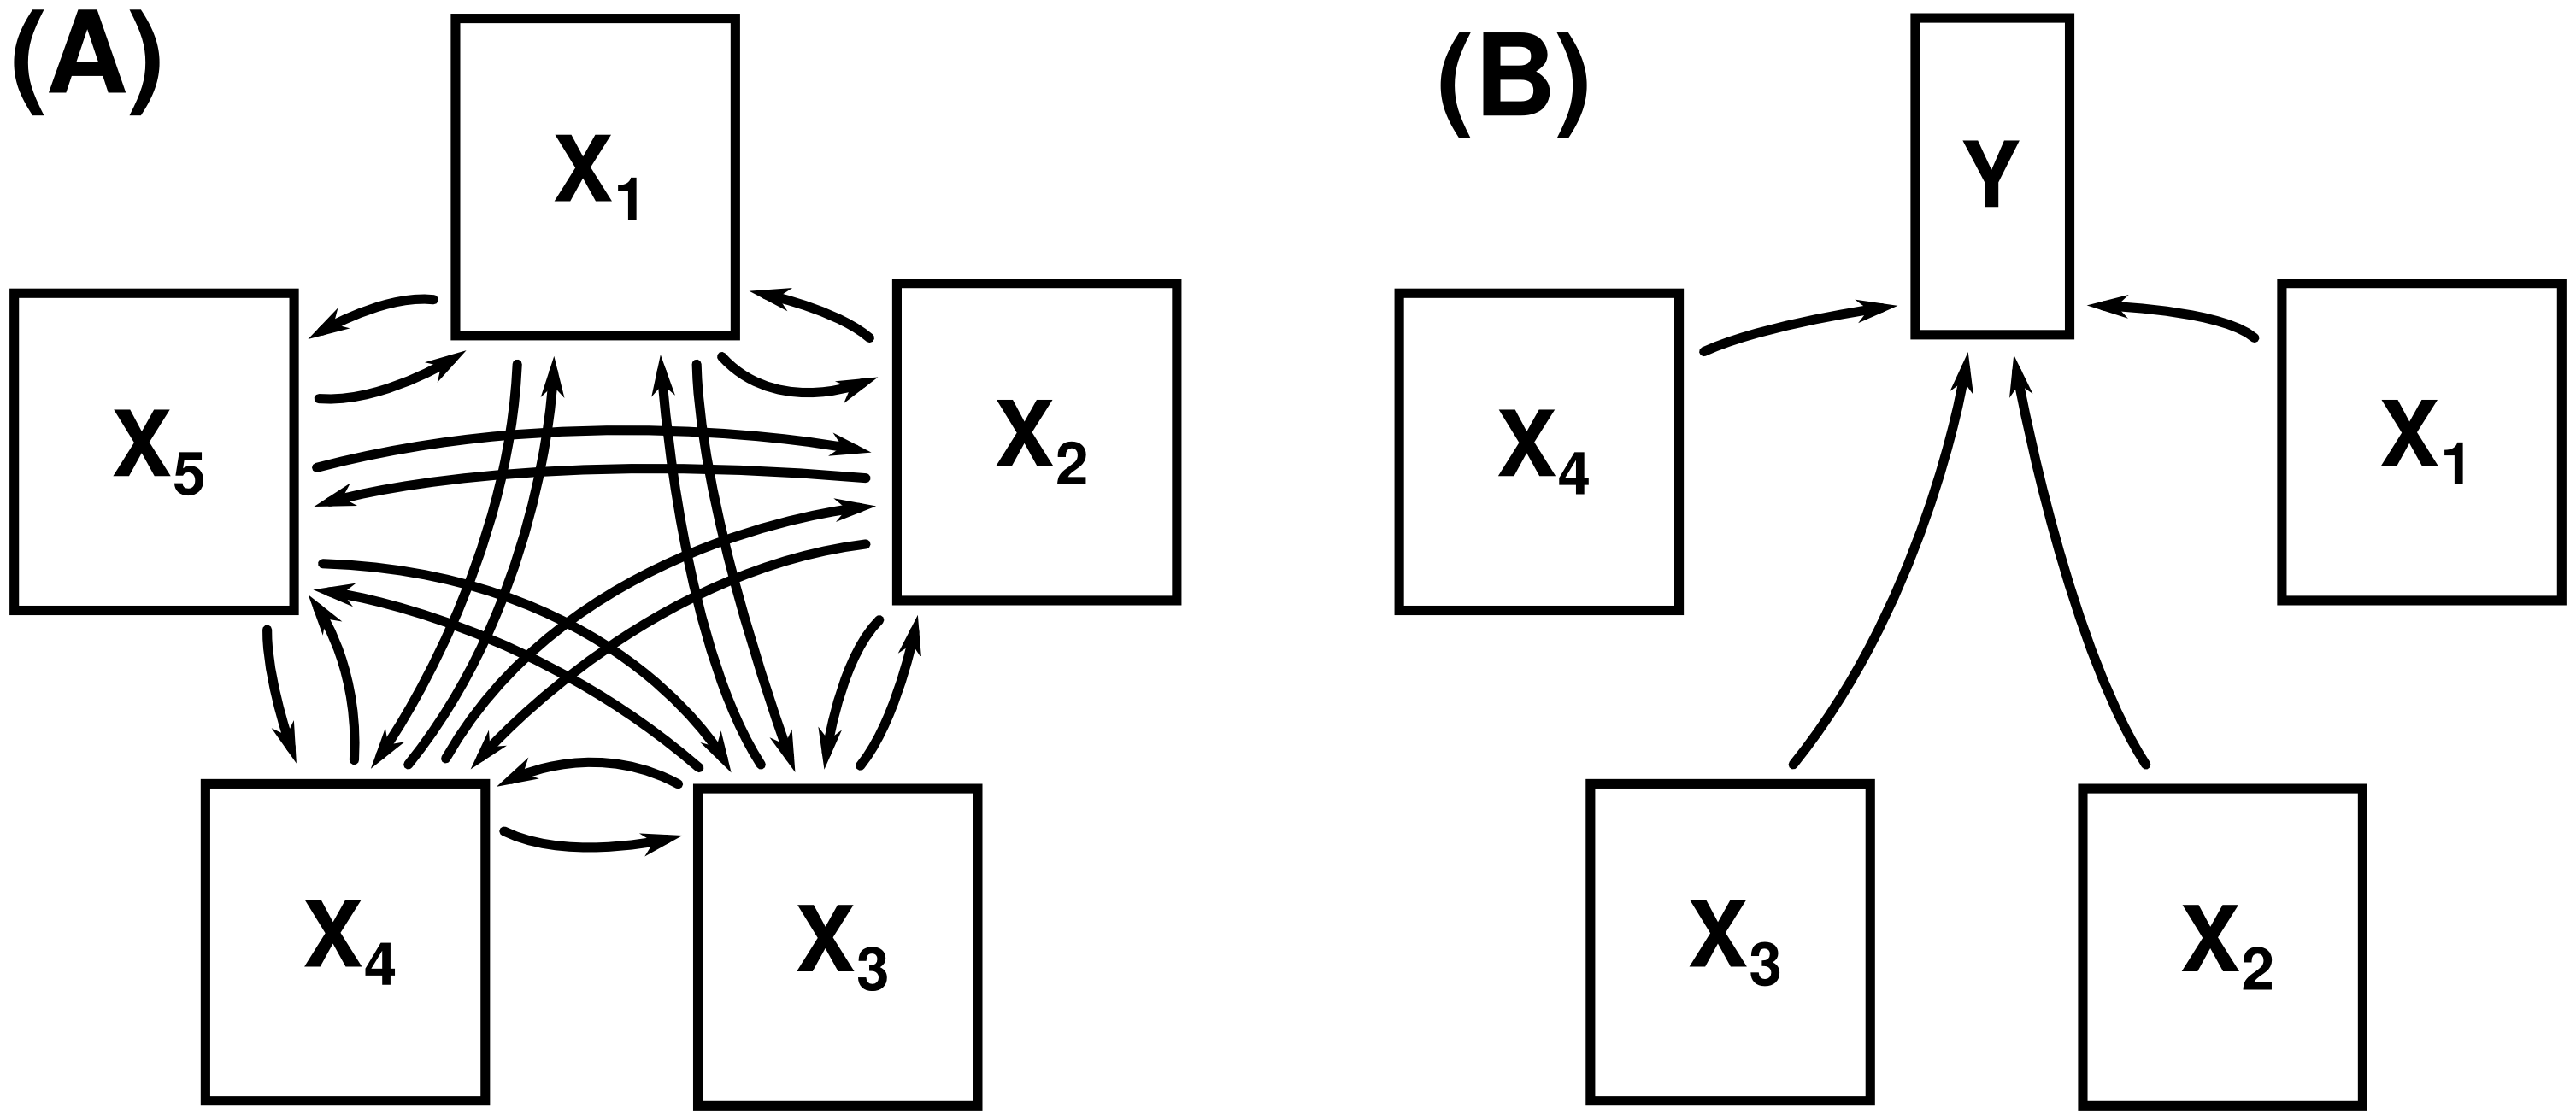
\includegraphics[width=5.5in]{figs/mva/13-assoc.png}
\end{center}
\caption
      [Association Graphs for OnPLS and MB-OPLS.]{
  {\bf Association Graphs for OnPLS and MB-OPLS.}
  \\
  ({\bf A}) Completely connected graph of nPLS and OnPLS regression models,
  illustrating how no single matrix is considered unique during training.
  ({\bf B}) Sparsely connected acyclic graph of MB-PLS and MB-OPLS regression
  models, where each data block $\mathbf{X}_b$ predicts a set of responses held
  in the unique matrix $\mathbf{Y}$.
}
\end{figure}

\begin{algorithm}[H]
\caption{Extraction of MB-OPLS Factors from OPLS}
\label{algorithm.3.7}
\begin{algorithmic}[1]
\REQUIRE $\mathbf{X}_b \in \mathbb{R}^{N \times K_b}
          \quad \forall b \in \ints{1}{B}$,%
       $\:\mathbf{Y} \in \mathbb{R}^{N \times M}$
\ENSURE $\mathbf{t} \in \mathbb{R}^N$,%
      $\:\mathbf{p} \in \mathbb{R}^K$,%
      $\:\mathbf{u} \in \mathbb{R}^N$,%
      $\:\mathbf{c} \in \mathbb{R}^M$,%
      $\:\mathbf{T_o} \in \mathbb{R}^{N \times a}$,%
      $\:\mathbf{P_o} \in \mathbb{R}^{K \times a}$, \\
      $\:\mathbf{t}_b \in \mathbb{R}^N$,%
      $\:\mathbf{p}_b \in \mathbb{R}^K$,%
      $\:\mathbf{T_o}_b \in \mathbb{R}^{N \times a}$,%
      $\:\mathbf{P_o}_b \in \mathbb{R}^{K \times a}
       \quad \forall b \in \ints{1}{B}$
\STATE $\{\mathbf{t}, \: \mathbf{p}, \: \mathbf{u}, \: \mathbf{c}, \:
        \mathbf{T_o}, \: \mathbf{P_o}\} \gets
        \mathrm{OPLS}(\mathbf{X}, \mathbf{Y})$
\FORALL{$b \in \ints{1}{B}$}
  \FORALL{$a_o \in \ints{1}{a}$}
    \STATE $\mathbf{t_o} \gets \mathbf{T_o}_{a_o}$ \COMMENT{
      Extract the $a_o$-th column of $\mathbf{T_o}$ }
    \STATE $\mathbf{w_o}_b \gets [\mathbf{W_o}_{a_o}]_b$ \COMMENT{
      Extract the $b$-th block of of $\mathbf{W_o}_{a_o}$ }
    \STATE $\mathbf{t_o}_b \gets \mathbf{X}_b \mathbf{w_o}_b$
    \STATE $\mathbf{p_o}_b \gets
            \tfrac{{\mathbf{X}_b}^T \mathbf{t_o}}
                  {\mathbf{t_o}^T \mathbf{t_o}}$
    \STATE $\mathbf{P_o}_b \gets [\mathbf{P_o}_b, \: \mathbf{p_o}_b]$
    \STATE $\mathbf{T_o}_b \gets [\mathbf{T_o}_b, \: \mathbf{t_o}_b]$
    \STATE $\mathbf{X}_b \gets \mathbf{X}_b - \mathbf{t_o} {\mathbf{p_o}_b}^T$
  \ENDFOR
  \STATE $\mathbf{w}_b \propto {\mathbf{X}_b}^T \mathbf{u}$
  \STATE $\mathbf{t}_b \gets \mathbf{X}_b \mathbf{w}_b$
  \STATE $\mathbf{p}_b \gets
          \tfrac{{\mathbf{X}_b}^T \mathbf{t}}
                {\mathbf{t}^T \mathbf{t}}$
  \STATE $\mathbf{X}_b \gets \mathbf{X}_b - \mathbf{t} {\mathbf{p}_b}^T$
\ENDFOR
\end{algorithmic}
\end{algorithm}

\begin{figure}[ht!]
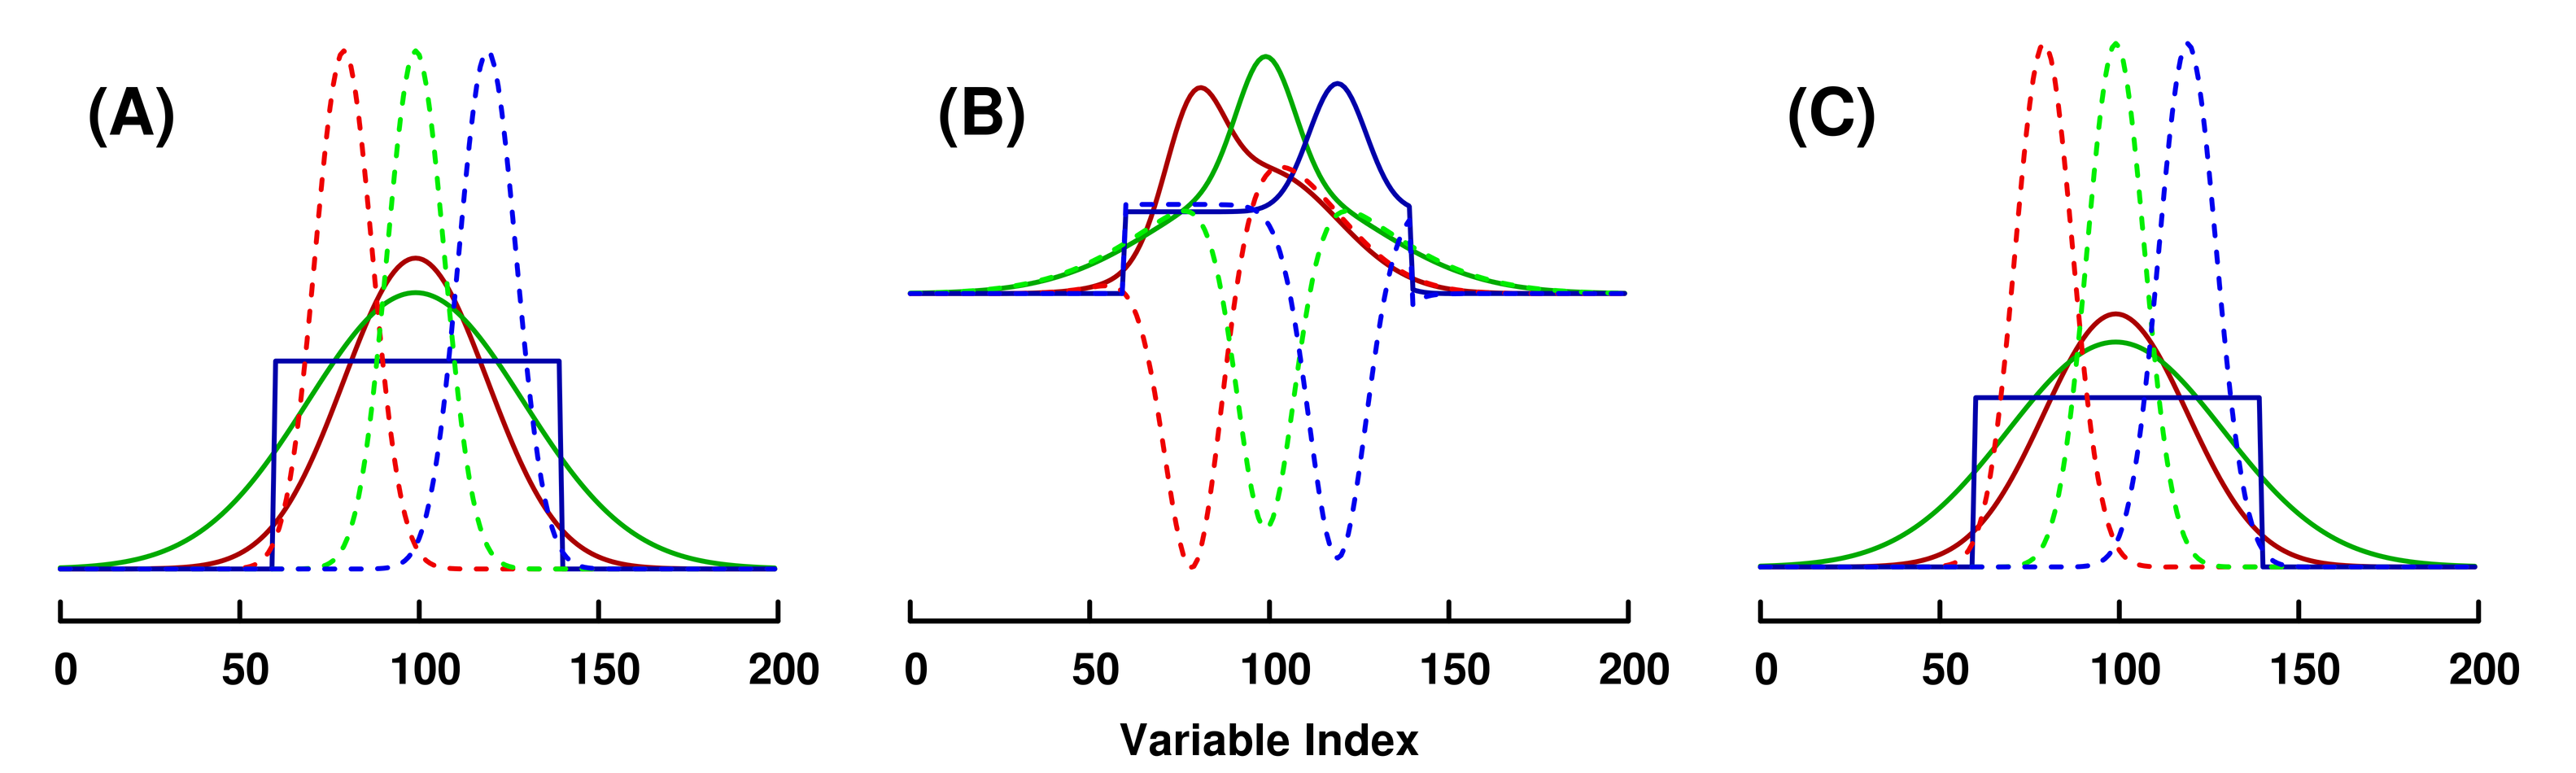
\includegraphics[width=6.5in]{figs/mva/14-mbopls.png}
\caption
      [Comparison of MB-PLS and MB-OPLS Loadings.]{
  {\bf Comparison of MB-PLS and MB-OPLS Loadings.}
  \\
  ({\bf A}) Original predictive (solid lines) and orthogonal (dashed lines)
  block loadings used to construct a toy three-block data structure having
  100 observations and 200 variables per block.
  ({\bf B}) Resulting MB-PLS block loadings from a two-component model,
  illustrating how the PLS algorithm mixes predictive information between
  multiple components in the presence of orthogonal variation.
  ({\bf C}) Resulting MB-OPLS predictive (solid) and orthogonal (dashed)
  block loadings from a one-component ($1+1$) model, effectively illustrating
  how MB-OPLS achieves the same segregation of predictive and orthogonal
  variation as OPLS and OnPLS on a per-block basis.
}
\end{figure}

\begin{doublespace}
For each of the $B$ data blocks, the extraction procedure first computes
orthogonal block loadings and scores, and deflates them from the block. Then,
predictive block scores and loadings are computed using the method outlined
previously \cite{westerhuis:jchemo1998} for extracting MB-PLS block components
from a PLS model (steps 12--14). The resulting block scores and loadings from
algorithm 3.7 are identical to those produced by algorithm 3.6.
\end{doublespace}

\section{Validation}

\begin{figure}[ht!]
\includegraphics[width=6.5in]{figs/mva/15-overfit.png}
\caption
      [Demonstration of PLS Overfit Based on Variable Count.]{
  {\bf Demonstration of PLS Overfit Based on Variable Count.}
  \\
  ({\bf A}) Scores from a two-component PLS model of unit-variance scaled
  Gaussian white noise ($N = 10$, $K = 5$). Inset: \rsqy{} (blue) and \qsq{}
  (green) statistics for each component in the model, computed from 100
  iterations of seven-fold Monte Carlo cross-validation.
  ({\bf B}) Same scenario as ({\bf A}) with $K = 10$.
  ({\bf C}) Same scenario as ({\bf A}) with $K = 20$.
  ({\bf D}) Same scenario as ({\bf A}) with $K = 100$.
}
\end{figure}

\begin{doublespace}
Application of the above bilinear factorization methods to one or more
spectral data matrices yields valuable insights into both general chemical
trends and relationships (e.g. from PCA) and response-predictive spectral
features (e.g. from OPLS) in those matrices. However, wanton use of these
multivariate methods without validation or knowledge of algorithmic intent
can quickly lead to statistically insignificant conclusions about the
underlying chemistry. The NIPALS-based algorithms described above are
highly numerically stable, even in the presence of multicollinearity,
noise, and missing data \cite{wold:cils2001,andersson:jchemo2009}. This
numerical stability almost guarantees that PCA, PLS and OPLS will return
a set of scores and loadings, even when those scores and loadings are only
based on a small fraction of the total variation in the data. PLS and OPLS
return biased regression coefficient estimates ($\hat{\mathbf{B}}_{PLS}$)
and force separation based on responses in scores space. OPLS is especially
adept at forcing scores-space separation, because its integrated OSC filter
removes systematic data matrix variation that does not ``agree'' with the
responses. These powerful modeling features make PLS and OPLS fully capable
of producing results based on noise alone, if so requested
\cite{westerhuis:metab2008a}. As the number of variables in the data increases
over the number of observations, the danger of overfitting also increases
(Figure 3.15). In effect, the probability of observing correlations to the
responses increases with variable count, just as the probability of observing
long runs of heads or tails increases with the number of fair coin tosses.
\\\\
In chemometric studies of spectroscopic datasets, where $N \ll K$, the tendency
of bilinear models to over-fit must be balanced by rigorous application of
several validation methods. When sufficient validation is lacking, any
conclusions drawn from these models should automatically be treated as
suspect from a statistical viewpoint. Therefore, all efforts must be taken
during experimental design, data collection and handling in order to obtain
data and models that acceptably withstand cross-validation.
\end{doublespace}

\subsection{Explained Variation}

\begin{doublespace}
In general, the amount of variation explained by a bilinear factorization of
a matrix is quantified by its sum of squares:
\begin{equation*}
SS \left\{ \mathbf{t} \mathbf{p}^T \right\} = \frosq{\mathbf{t} \mathbf{p}^T}
\end{equation*}
where $\frosq{\cdot}$ denotes the squared Frobenius norm, which will be used
as a shorthand for the sum of squares. Because the raw sum of squares is not
scale-invariant, it is normally reported as a ratio relative to the total sum
of squares. In the context of a PCA (equation 3.20), this ratio is referred
to as \rsqx{} (or simply \rsq{}):
\begin{align}
R^2_X
 =& \: \frac{\ssfit{}}{\sstot{}}
     = \frac{\frosq{\mathbf{T} \mathbf{P}^T}}{\frosq{\mathbf{X}}} \\
 =& \: 1 - \frac{\sserr{}}{\sstot{}}
     = 1 - \frac{\frosq{\mathbf{E}}}{\frosq{\mathbf{X}}}
\end{align}
where the second set of equalities arises from the fact that PCA loadings are
eigenvectors of $\mathbf{X}^T \mathbf{X}$ and right singular vectors of
$\mathbf{X}$ \cite{jolliffe2002}. The cumulative \rsqx{} statistic may be
broken into sums of per-component \rsqx{} statistics, due to the orthonormality
properties of principal components:
\begin{equation}
R^2_X =
 \sum_{a=1}^A
 \frac{\frosq{\mathbf{t}_a {\mathbf{p}_a}^T}}
      {\frosq{\mathbf{X}}}
\end{equation}

In the case of PLS modeling (equation 3.37), a similar ratio exists (\rsqy{})
that quantifies the amount of variation explained in the responses:
\begin{align}
R^2_Y
 =& \: \frac{\frosq{\mathbf{T} \mathbf{C}^T}}{\frosq{\mathbf{Y}}} \\
 =& \: 1 - \frac{\frosq{\mathbf{F}}}{\frosq{\mathbf{Y}}}
\end{align}

Similar expressions exist for the predictive and orthogonal factorizations of
$\mathbf{X}$ in OPLS models, which are referred to as \rsqxp{} and \rsqxo{},
respectively. While these \rsq{} statistics provide valuable first insights
into the amount of variation that may be explained by a given model framework,
they are gross over-estimations of model reliability and should not be used
during model selection as a means of determining the optimal component count,
$A^\ast$. Cross-validatory methods discussed in later sections provide more
effective means of identifying $A^\ast$ during model training.
\end{doublespace}

\subsection{External Cross-validation}

\begin{doublespace}
In its most traditional form, cross-validation involves the division of $N$
observations in a dataset (i.e. $\mathbf{X}$ and $\mathbf{Y}$) into a training
set ($\mathbf{X}_t$ and $\mathbf{Y}_t$) having $N_t$ observations and a
validation set ($\mathbf{X}_v$ and $\mathbf{Y}_v$) having $N_v$ observations.
The training and validation datasets are then processed and treated separately
using identical methods, and models are constructed on the training dataset.
In the case of PLS modeling, the analyst will arrive at the following equation:
\begin{equation}
\mathbf{Y}_t = \mathbf{X}_t \mathbf{W}^\ast \mathbf{C}^T + \mathbf{F}
\end{equation}

Assessment of model reliability is then performed by estimating the responses
of the validation dataset using the trained model, like so:
\begin{equation}
\hat{\mathbf{Y}}_v = \mathbf{X}_v \mathbf{W}^\ast \mathbf{C}^T
\end{equation}
where the predicted residual sum of squares (PRESS) statistic is now readily
computable from the sum of squares of the difference between true and estimated
validation-set responses:
\begin{equation}
\mathrm{PRESS} = \frosq{\mathbf{Y}_v - \hat{\mathbf{Y}}_v}
\end{equation}

A scale-invariant reporter of reliability (\qsq{}) is obtained from the PRESS
statistic as follows:
\begin{equation}
Q^2
 = 1 - \frac{\mathrm{PRESS}}{\sstot{}}
 = 1 - \frac{\frosq{\mathbf{Y}_v - \hat{\mathbf{Y}}_v}}{\frosq{\mathbf{Y}_v}}
\end{equation}

This model reliability statistic is often referred to as a ``cross-validated''
\rsq{} statistic, and provides a relative measure of how well a given model
will generalize to the estimation of future observations. Like \rsq{}
statistics, \qsq{} is also computable on a per-component basis.
\end{doublespace}

\subsection{Internal Cross-validation}

\subsubsection{Supervised Models}

\begin{doublespace}
Due to the severely limited number of observations in most chemometric studies,
the practice of external cross-validation is rare, and all observations are
usually retained for model training. Nevertheless, model reliability statistics
may be obtained from the similar practice of \emph{internal} cross-validation.
In any internal cross-validation scheme, the $N$ observations of a given
dataset are divided into $G$ groups, referred to as $G$-fold or
leave-$n$-out cross-validation (where $n = \lfloor N / G \rfloor$). Each
group is then left out in turn, and its responses are estimated from a model
trained on the remainder of the data. To more succinctly introduce internal
cross-validation procedures, the set of all partitionings of $N$ elements into
$G$ groups, denoted $\mathbb{P}(N, G)$, shall be introduced:
\begin{equation}
\mathbb{P}(N, G) \equiv \big\{
 \mathbf{p} \mid \mathbf{p} \in \mathbb{Z}^N
 \wedge
 1 \le p_n \le G
 \quad \forall n \in \ints{1}{N}
\big\}
\end{equation}

As an example, one member of the set $\mathbb{P}(7, 3)$ is $(1,2,3,1,2,3,1)$.
Given a partitioning $\boldsymbol{\sigma} \in \mathbb{P}(N, G)$, the following
algorithm demonstrates the computation of \qsq{} for a single PLS component:
\end{doublespace}

\begin{algorithm}[H]
\caption{Internal PLS Component Cross-validation}
\label{algorithm.3.8}
\begin{algorithmic}[1]
\REQUIRE $\mathbf{X} \in \mathbb{R}^{N \times K}$,%
       $\:\mathbf{Y} \in \mathbb{R}^{N \times M}$,%
       $\:G$, $\:\boldsymbol{\sigma} \in \mathbb{P}(N, G)$
\ENSURE $Q^2 \in \mathbb{R}$
\FORALL{$g \in \ints{1}{G}$}
  \STATE $n_g \gets \{ n \mid n \in \ints{1}{N} \wedge \sigma_n = g \}$
  \STATE $\{\mathbf{t}, \mathbf{p}, \mathbf{u}, \mathbf{c}, \mathbf{w}\}
          \gets \mathrm{PLS}(\mathbf{X}^{(-n_g)},
                             \mathbf{Y}^{(-n_g)})$ \COMMENT{
 $\mathbf{X}^{(-n_g)}$, $\mathbf{Y}^{(-n_g)}$ contain no rows from group $g$
}
  \STATE $\mathbf{B}^{(g)} \gets \tfrac{\mathbf{w} \mathbf{c}^T}
                                       {\mathbf{p}^T \mathbf{w}}$
\ENDFOR
\FORALL{$n \in \ints{1}{N}$}
  \STATE $\hat{\mathbf{y}}_n \gets
          \mathbf{x}_n \mathbf{B}^{(\sigma_n)}$ \COMMENT{
 $\hat{\mathbf{y}}_n$, $\mathbf{x}_n$ are the $n$-th rows of
 $\hat{\mathbf{Y}}$, $\mathbf{X}$
}
\ENDFOR
\STATE $Q^2 \gets 1 - \frac{\frosq{\mathbf{Y} - \hat{\mathbf{Y}}}}
                           {\frosq{\mathbf{Y}}}$
\end{algorithmic}
\end{algorithm}

\begin{doublespace}
In the simplest case where $G = N$, known as leave-one-out cross-validation
(LOOCV), only one observation is left out at a time. It has been shown,
however, that leave-one-out methods do not identify optimal models as
effectively as leave-$n$-out methods as $N$ increases \cite{shao:jasa1993},
so $G$ should be less than the number of observations whenever possible.
Within a leave-$n$-out cross-validation of $N$ observations, there are
$\binom{N}{n}$ different ways to partition the dataset into the desired
number of groups. A complete cross-validation would require the evaluation
of all possible partitions, which is computationally intractable even for
small (e.g. $N \ge 20$) datasets. While it is possible to arbitrarily select
a single partitioning, such as a regular pattern of group assignment, it is
much more attractive to randomly resample a number of partitionings ($n_p$)
from the set of $\binom{N}{n}$ possibilities
($\boldsymbol{\sigma} \sim \mathbb{P}(N,G)$) in a
Monte Carlo leave-$n$-out cross-validation approach \cite{xu:cils2001}. Monte
Carlo cross-validation offers the possibility of assigning confidence regions
to reported \qsq{} values for a given dataset, which provides the analyst with
further information on model reliability estimates.
\\\\
In practice, per-component \qsq{} statistics provide a means of determining
$A^\ast$, the optimal component count. When new components are added to the
model that fail to reliably estimate the responses under cross-validation,
their \qsq{} values will become negative. Thus, a practical rule during model
training is to only retain components having positive \qsq{} statistics.
\end{doublespace}

\begin{figure}[h!]
\begin{center}
  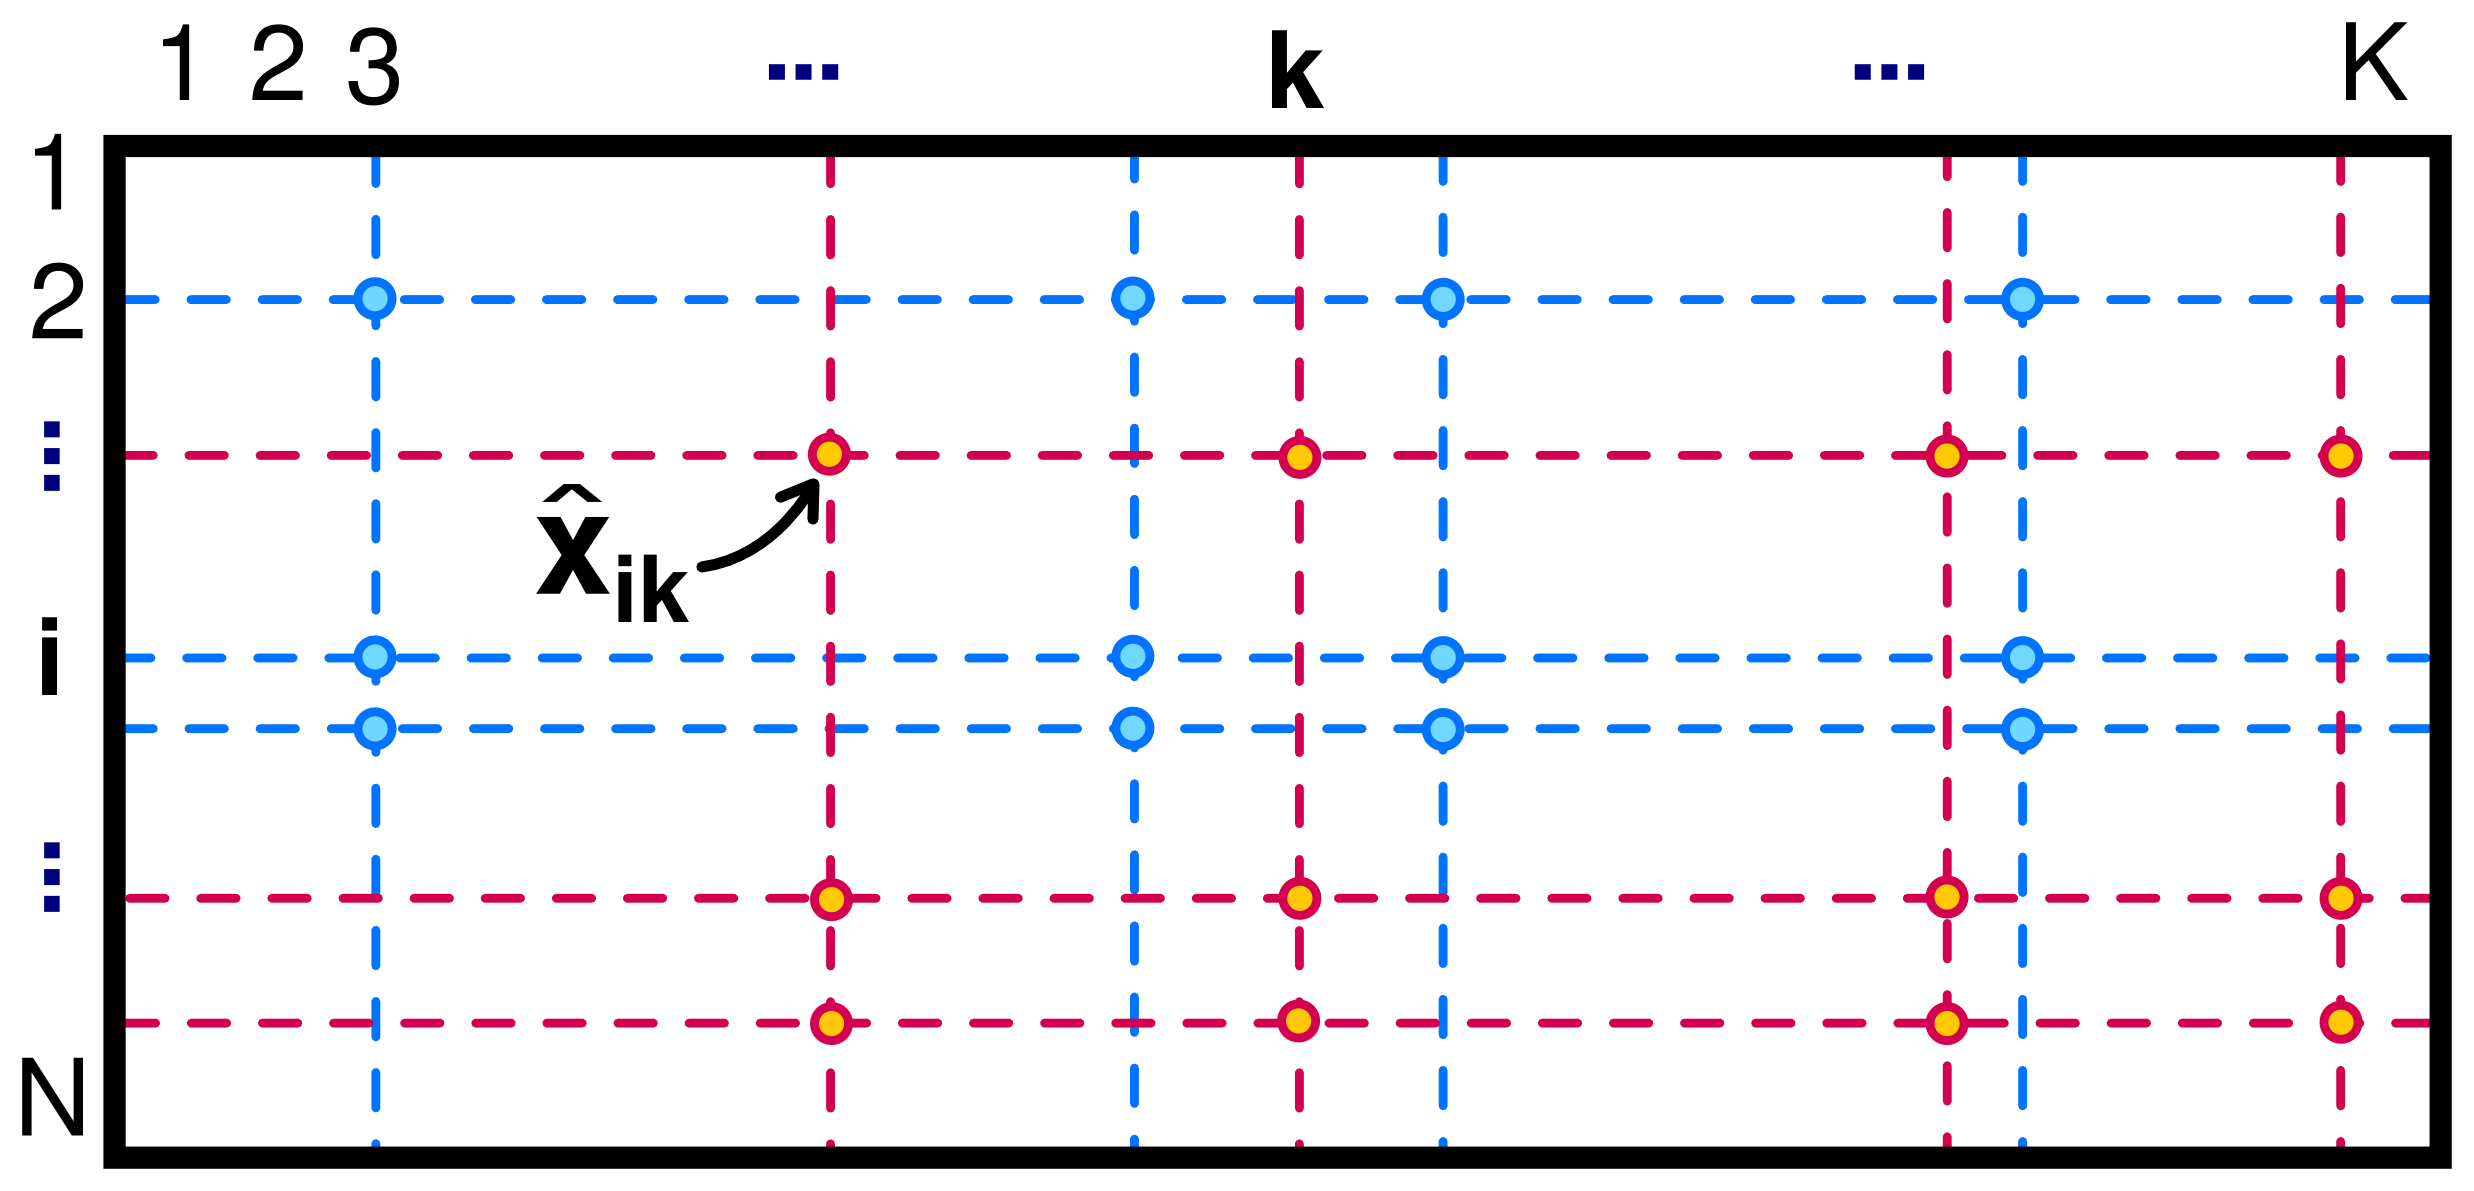
\includegraphics[width=4.5in]{figs/mva/16-pcacv.png}
\end{center}
\caption
      [Partitioning in Leave-$n$-out PCA Cross-validation.]{
  {\bf Partitioning in Leave-$n$-out PCA Cross-validation.}
  \\
  Graphical illustration of two different partitionings (red and blue) of a
  data matrix. Each partitioning (group) requires the computation of a set of
  scores ($\hat{\mathbf{t}}$) and loadings ($\hat{\mathbf{p}}$) in order to
  estimate it's left-out values, indicated by filled circles. Estimation of
  $\hat{x}_{ik}$ requires computation of $\hat{\mathbf{t}}$ with variable $k$
  left out and $\hat{\mathbf{p}}$ with observation $i$ left out. The value of
  $\hat{x}_{ik}$ is then obtained from the $(i,k)$-th index of
  $\hat{\mathbf{t}} \hat{\mathbf{p}}^T$
}
\end{figure}

\subsubsection{Unsupervised Models}

\begin{doublespace}
Internal cross-validation of unsupervised PCA models poses a unique challenge
in comparison to PLS and OPLS, as it does not involve prediction of a set of
responses \cite{eastment:tech1982,krzanowski:biom1987,eshghi:cils2014}. Eshghi
\cite{eshghi:cils2014} provides a more comprehensive review of internal
cross-validation practices for PCA models. In short, leave-$n$-out
cross-validation of PCA models requires that both observations \emph{and}
variables be partitioned into $G$ groups. The resulting pair of partitionings
allows groups of data matrix elements to be left out and recomputed during
cross-validation. For each group, a score vector $\hat{\mathbf{t}}$ is
computed after leaving out variables in the group, and a loading vector
$\hat{\mathbf{p}}$ is computed after leaving out observations in the group.
The outer product of $\hat{\mathbf{t}}$ and $\hat{\mathbf{p}}$ is then used
in estimating the data matrix elements located at the intersections of the
left-out variables and observations (Figure 3.16). The following algorithm
demonstrates the computation of \qsq{} for a single principal component, given
a row partitioning $\boldsymbol{\sigma}$ and a column partitioning
$\boldsymbol{\rho}$:
\end{doublespace}

\begin{algorithm}[H]
\caption{Internal PCA Component Cross-validation}
\label{algorithm.3.9}
\begin{algorithmic}[1]
\REQUIRE $\mathbf{X} \in \mathbb{R}^{N \times K}$, $\:G$,
       $\:\boldsymbol{\sigma} \in \mathbb{P}(N, G)$,%
       $\:\boldsymbol{\rho} \in \mathbb{P}(K, G)$
\ENSURE $Q^2 \in \mathbb{R}$
\FORALL{$g_1 \in \ints{1}{G}$}
  \STATE $n_g \gets \{ n \mid n \in \ints{1}{N} \wedge \sigma_n = g_1 \}$
    \STATE $\hat{\mathbf{p}} \gets \mathrm{PCA}(\mathbf{X}^{(-n_g)})$ \COMMENT{
    $\mathbf{X}^{(-n_g)}$ contains no rows from group $g$}

  \FORALL{$g_2 \in \ints{1}{G}$}
    \STATE $k_g \gets \{ k \mid k \in \ints{1}{K} \wedge \rho_k = g_2 \}$
    \STATE $\hat{\mathbf{t}} \gets \mathrm{PCA}(\mathbf{X}^{(-k_g)})$ \COMMENT{
    $\mathbf{X}^{(-k_g)}$ contains no columns from group $g$}
    \STATE $\hat{\mathbf{t}} \gets \hat{\mathbf{t}}
            \sqrt{\tfrac{K}{K - |k_g|}}$
    \FORALL{$n \in n_g$}
      \FORALL{$k \in k_g$}
        \STATE $\hat{\mathbf{X}}_{n,k} \gets
                \hat{\mathbf{t}}_n \hat{\mathbf{p}}_k$
      \ENDFOR
    \ENDFOR
  \ENDFOR
\ENDFOR
\STATE $Q^2 \gets 1 - \frac{\frosq{\mathbf{X} - \hat{\mathbf{X}}}}
                           {\frosq{\mathbf{X}}}$
\end{algorithmic}
\end{algorithm}

\subsection{Response Permutation Testing}

\begin{doublespace}
While internal cross-validation metrics such as \qsq{}, number of
misclassifications, and AUROC \cite{westerhuis:metab2008a} are a good first
insight into model reliability, they do not provide a robust mechanism for
discriminating between low- and high-quality models. Methods that report a
degree of statistical significance in the form of a $p$ value are preferred,
as they may be compared to a threshold (e.g. $\alpha = 0.05$). One such method,
known as response permutation testing, establishes a distribution of models
representing the null hypothesis ($H_0$) that no relationship exists between
the data and responses \cite{westerhuis:metab2008a}. For a number of
iterations, the rows of the response matrix $\mathbf{Y}$ are randomly permuted
to yield a null response matrix $\tilde{\mathbf{Y}}$, upon which a supervised
PLS or OPLS model is trained. The set of models generated after response
permutation -- more specifically their \rsq{} and \qsq{} parameters -- may be
compared against those of the original model to obtain a $p$ value. Provided
the resulting $p$ value is less than the defined threshold $\alpha$, the
analyst may reject the null hypothesis that the original model is based on
random correlations between $\mathbf{X}$ and $\mathbf{Y}$.
\end{doublespace}

\subsection{CV-ANOVA Testing}

\begin{doublespace}
Response permutation testing capably reports $p$ values via hypothesis testing
of model reliability, but it requires significant computation time to train
the 100 -- 1,000 models required for an accurate result. The alternative
CV-ANOVA testing method effectively requires no additional computation time
after internal cross-validation, as it compares the fitted $\mathbf{Y}$
residuals obtained from cross-validation procedures \cite{eriksson:jchemo2008}.
In effect, CV-ANOVA tests whether the mean square error of fitted residuals
from PLS and OPLS models is significantly smaller than the total mean square
variation in $\mathbf{Y}$. By comparing the ratio of these mean square values
to an $F$ distribution, CV-ANOVA reports its own $p$ value which may again be
compared to a threshold.
\end{doublespace}

\section{Conclusions}

\begin{doublespace}
Multivariate bilinear factorizations such as PCA, PLS and OPLS provide an
essential platform for rapid information extraction of rich spectral datasets.
Through proper application of processing and treatment, optimal choice of
modeling algorithms, and judicious administration of validation metrics,
multivariate analysis can lend a powerful hand in biochemical examination of
complex, multiparametric metabolic systems. Specific applications of
multivariate analysis in metabolomics are discussed in further detail in the
following chapter.
\end{doublespace}

\bibliographystyle{abbrv}
\bibliography{bworley}



\chapter{Applications of Multivariate Analysis in Metabolomics}

\section{Introduction}

\begin{doublespace}
This chapter details several varied applications of multivariate analysis
within the field of metabolomics, from the simplest examples of constructing
multivariate calibration models of \hnmr{} NMR spectral data for determination
of caffeine concentration in coffee, to more complex examples of multiblock
statistical modeling of joint \hnmr{} NMR and electrospray MS data. A final
note on the relationship between PCA scores-space class separations and OPLS-DA
model reliability is also presented to conclude the chapter.
\end{doublespace}

\section{\hnmr{} NMR Fingerprinting of Brewed Coffees}

\begin{doublespace}
To provide an initial illustration of the capabilities of the MVAPACK software
suite \cite{worley:acscb2014}, four roasts of brewed coffee were purchased from
a local coffee shop. In this study, \hnmr{} NMR and UV/Vis absorbance spectra
were collected in order to construct a multivariate calibration of \hnmr{} NMR
spectral information against caffeine concentration.
\end{doublespace}

\subsection{Materials and Methods}

\subsubsection{Coffee Sample Preparation}

\begin{doublespace}
Four freshly brewed roasts of coffee (Light, Dark, Medium Regular and Medium
Decaffeinated) were purchased from a local coffee shop. From each roast,
sixteen 1.2 mL samples were drawn while the coffee was still hot and stored
at $-80^\circ$C for 24 hours. The samples were then lyophilized at
$-50^\circ$C and 0.1 mBar for 24 hours and subsequently redissolved in 1.0 mL
of 99.8\% D$_2$O (Isotec, St. Louis, MO) without pH adjustment. Following
redissolution, the samples were centrifuged at 12,000 RPM and $25^\circ$C
for 5 minutes and 800 $\mu$L of the supernatant was collected into NMR tubes.
The samples were stored in their NMR tubes at $4^\circ$C for 36 hours prior
to data collection.
\end{doublespace}

\subsubsection{Caffeine Extraction}

\begin{doublespace}
Measurement of the caffeine concentration in each coffee roast was performed
based on previously outlined procedures \cite{belay:food2008}. Triplicate
standards of caffeine were made by dissolving 2.9 mg of caffeine
(Sigma-Aldrich, St. Louis, MO) into 100.0 mL of 99.5\% CH$_2$Cl$_2$
(Sigma-Aldrich, St. Louis, MO) for a final concentration of 149 $\mu$M.
From each purchased coffee roast, 25 mL of brewed coffee were combined with
25 mL of CH$_2$Cl$_2$ in a separatory funnel in a two-step liquid-liquid
extraction. Extracted caffeine in CH$_2$Cl$_2$ was diluted 20-fold into 1.0
mL and subjected to UV/Vis absorption spectroscopy for caffeine quantitation.
\end{doublespace}

\begin{figure}[ht!]
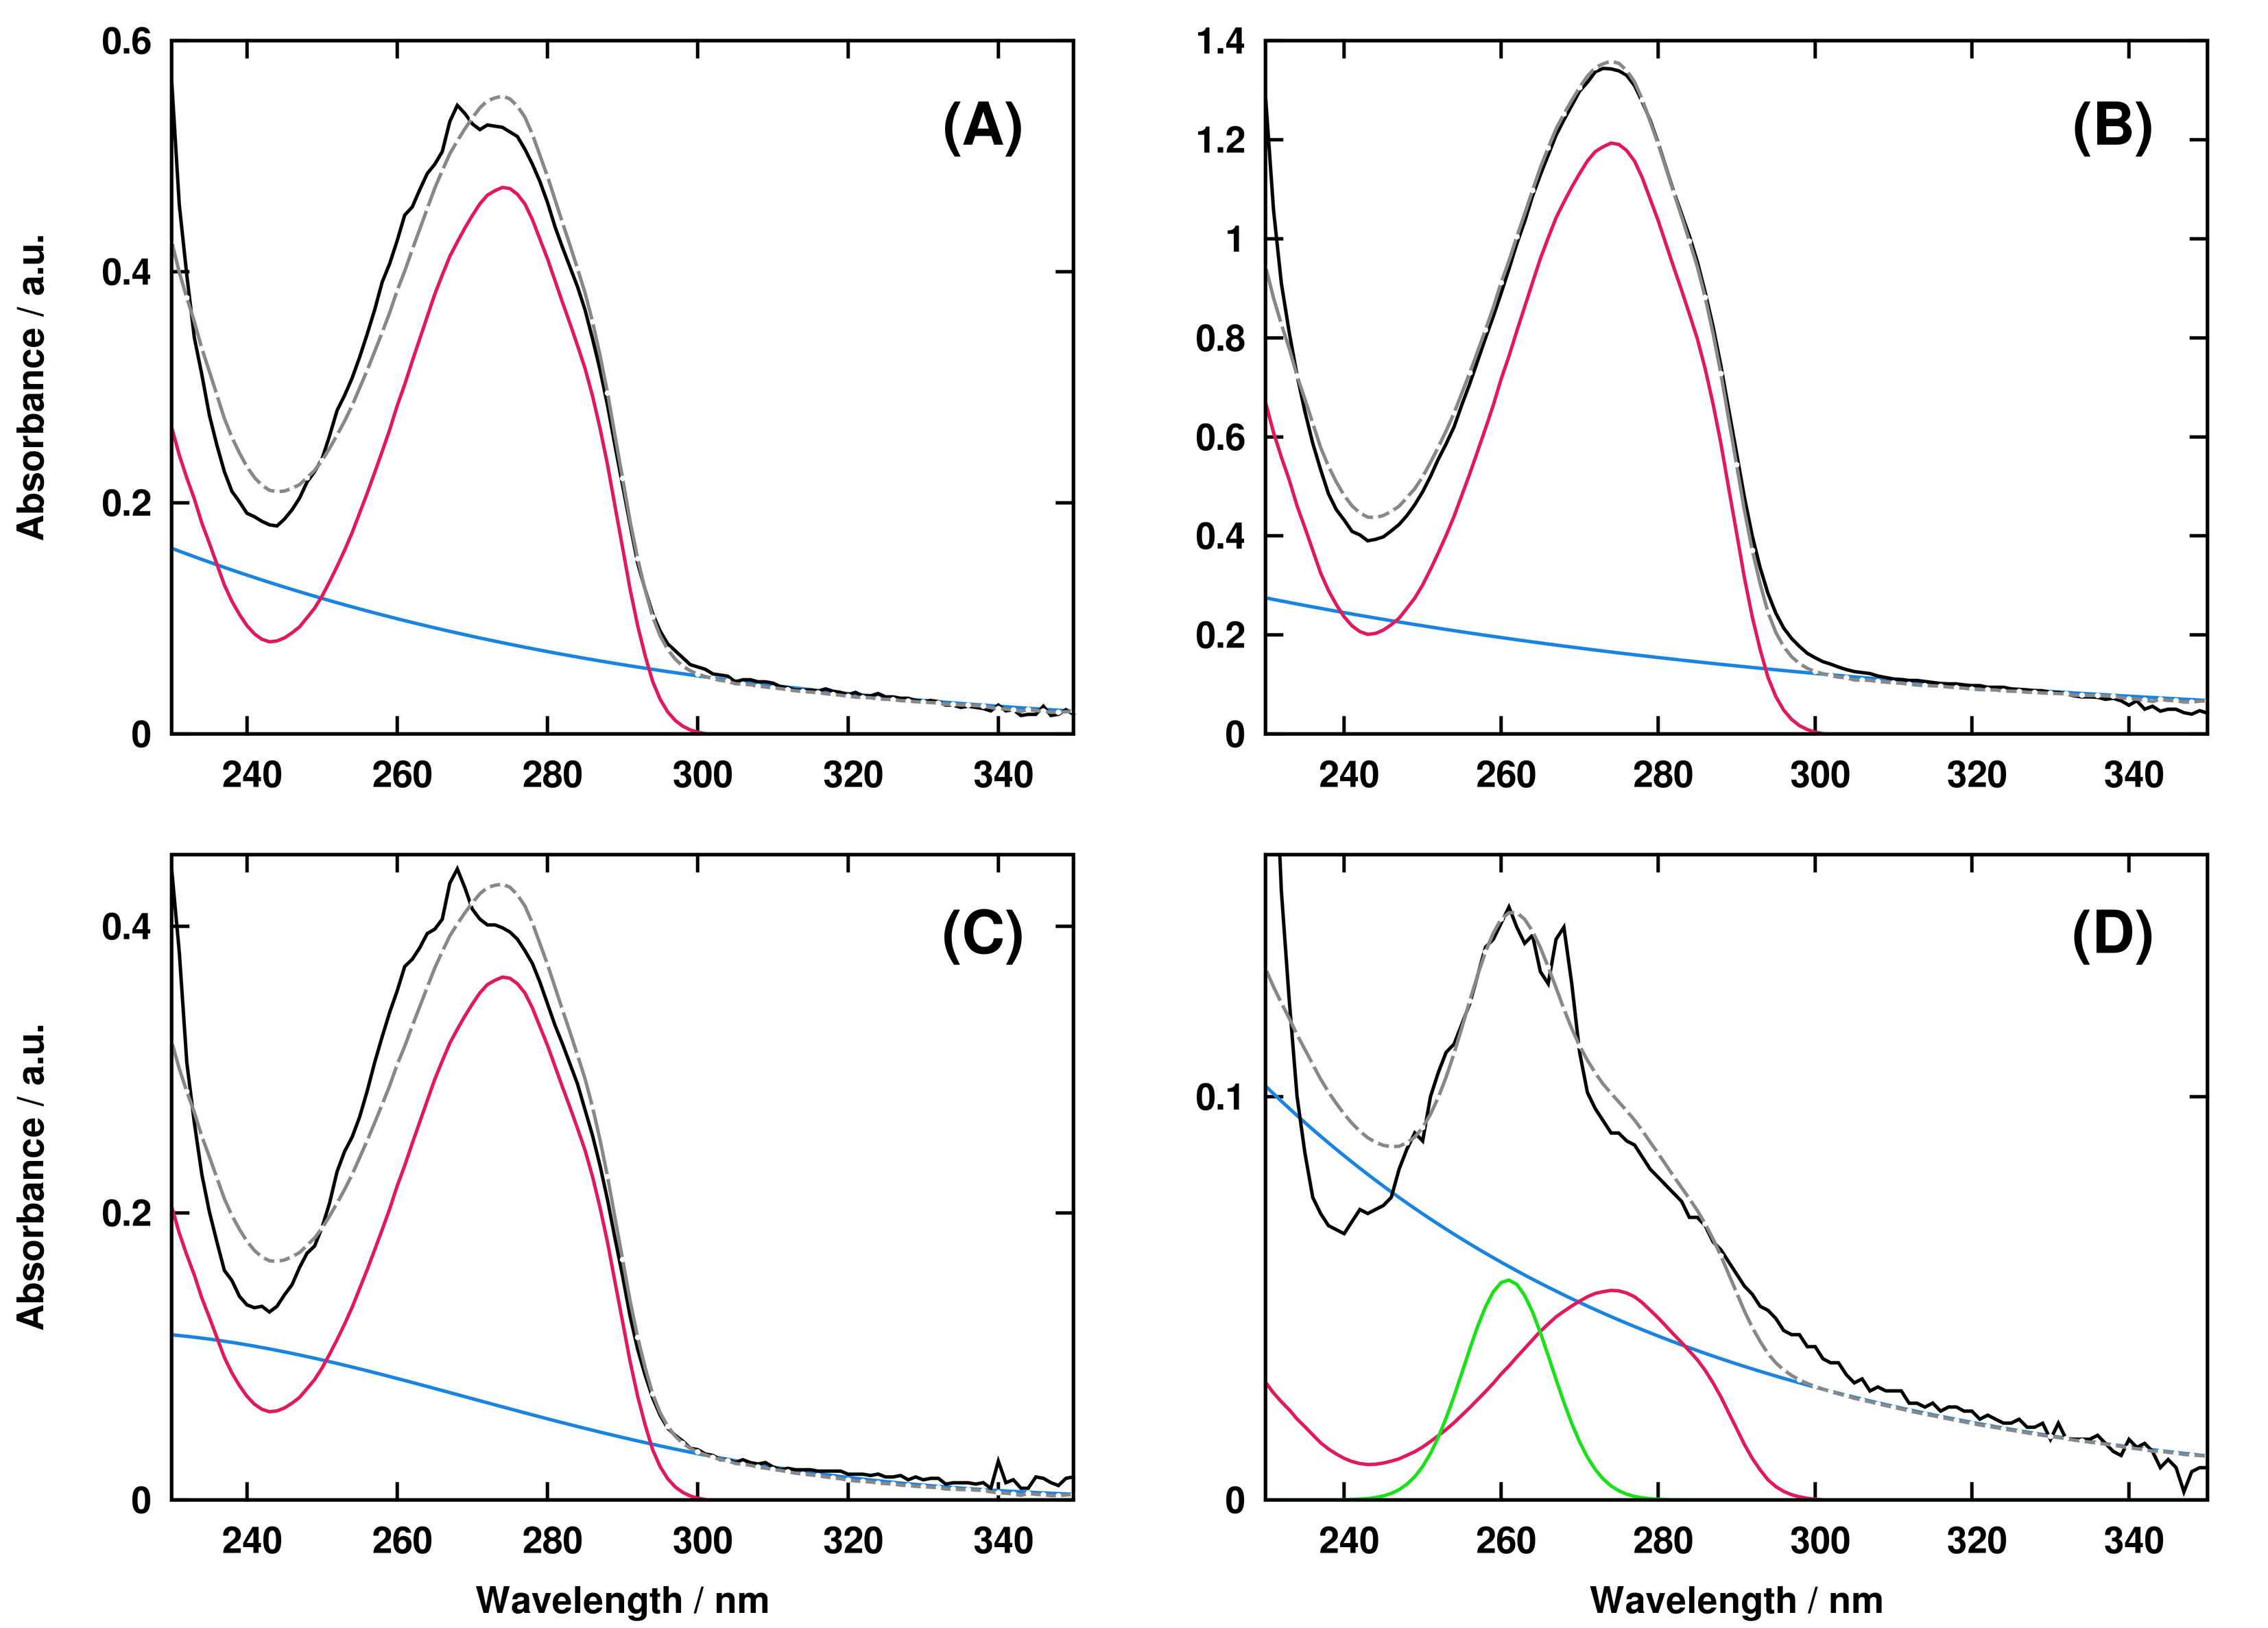
\includegraphics[width=6.5in]{figs/apps/01-uvfit.png}
\caption
      [UV/Vis Caffeine Quantitation Band-fitting Results.]{
  {\bf UV/Vis Caffeine Quantitation Band-fitting Results.}
  \\
  UV/Vis absorbance band-fitting results for caffeine concentration estimation
  of dark roast ({\bf A}), light roast ({\bf B}), regular medium roast
  ({\bf C}), and decaffeinated medium roast ({\bf D}). Black lines represent
  observed spectra, dashed grey lines represent fitted spctra, red lines
  represent fitted caffeine, and blue and green lines represent additional
  Gaussian bands required for fitting.
}
\end{figure}

\subsubsection{UV/Vis Spectroscopy}

\begin{doublespace}
Absorption spectra of caffeine standards and extracts were collected on a
Shimadzu UV-2501PC with a 1.0 nm slit width and 1.0 cm quartz cuvettes. Spectra
were collected between the wavelengths of 500 nm and 230 nm.
\end{doublespace}

\subsubsection{NMR Spectroscopy}

\begin{doublespace}
All NMR experiments were collected on a Bruker Avance DRX 500 MHz spectrometer
equipped with a 5 mm inverse triple-resonance (\hnmr{}, \cnmr{}, \nnmr{})
cryoprobe with a $z$-axis gradient. A Bruker BACS-120 sample changer and
ICON-NMR software were used to automate NMR data collection. A standard 1D
\hnmr{} NMR spectrum using a SOGGY pulse sequence
\cite{hwang:jmr1995,nguyen:jmr2007} and a $T_2$-filtered 1D \hnmr{} NMR
spectrum using a $z$-filtered Carr-Purcell-Meiboom-Gill (CPMG) sequence
\cite{rastrelli:jacs2009} with an identical SOGGY water suppression element
were acquired for each sample. All experiments were performed at $20^\circ$C
with 128 scans, 32 dummy scans, a carrier frequency offset of 2,351 Hz, a
6,009 Hz spectral width, and a 1.0 s inter-scan delay. For $T_2$ filtered
spectra, 20 repetitions of a CPMG-$z$ element having a delay ($\tau$) of 5.0
ms were performed per scan, for a total filter time ($2n\tau$) of 200.0 ms.
Free induction decays were collected with 32,768 total data points resulting
in a total acquisition time of 10 minutes per experiment.
\end{doublespace}

\subsubsection{Caffeine Quantitation}

\begin{doublespace}
A reference spectrum of caffeine in CH$_2$Cl$_2$ was generated from the three
standard UV/Vis absorption spectra by taking the mean of the spectra after
multiplicative scatter correction (MSC, \cite{fearn:cils2009}). To quantify
caffeine in the extracts, the absorption spectrum of each extract was fit by
nonlinear least squares \cite{marquardt:jsiam1963} to the sum of the scaled
caffeine reference spectrum and no more than two extra `background' Gaussian
bands (Figure 4.1). The ratio of the fit caffeine reference spectrum in each
extract to that of the known samples was used as an estimate of caffeine
concentration in the extracts. Concentrations of the medium regular, medium
decaffeinated, dark and light roasts were 1.526 mM, 0.217 mM, 1.979 mM and
4.993 mM, respectively.
\end{doublespace}

\subsubsection{Multivariate Analysis}

\begin{doublespace}
All NMR spectra were loaded, processed, treated and modeled inside the GNU
Octave 3.6 programming environment \cite{eaton2008} using functions available
in the MVAPACK software suite for chemometrics \cite{worley:acscb2014}.
Free induction decays were loaded in from Bruker DMX binary format and
corrected for group delay errors by a circular shift of their time-domain
data points. All decays were Fourier transformed, automatically phase-corrected
and referenced to match the chemical shifts of caffeine with known database
values. Spectral regions upfield of 0.44 ppm and downfield of 9.16 ppm were
removed from the dataset, as they contained no informative signals. As solvent
resonances were adequately suppressed by the excitation sculpting pulse
sequence, no spectral regions were removed around the water resonance.
Figure 4.2 illustrates the final result of spectral processing of the coffees
dataset using MVAPACK.
\end{doublespace}

\begin{figure}[ht!]
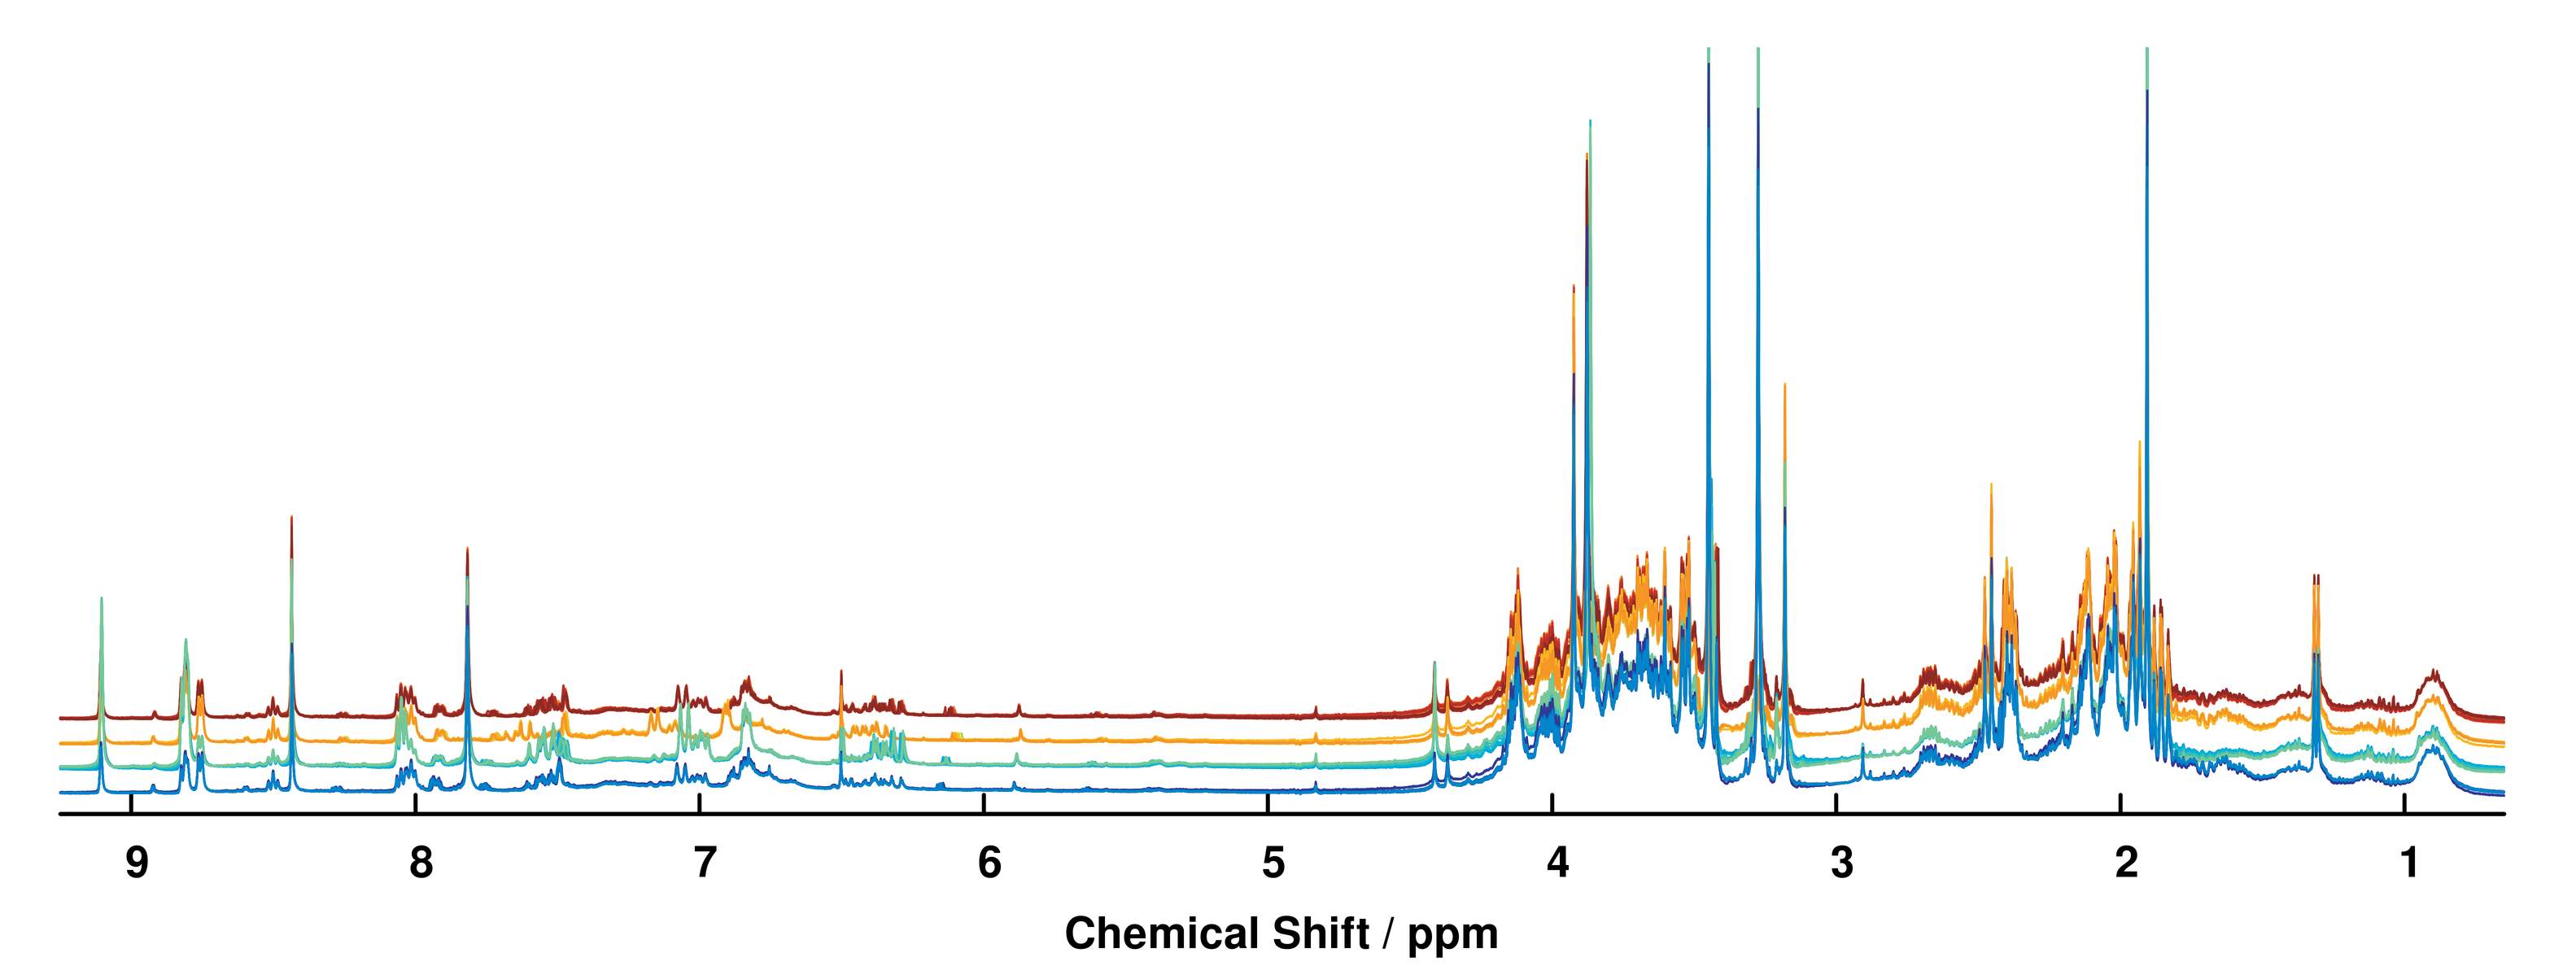
\includegraphics[width=6.5in]{figs/apps/02-spectra.png}
\caption
      [Processed \hnmr{} NMR Spectra of Coffee Roasts.]{
  {\bf Processed \hnmr{} NMR Spectra of Coffee Roasts.}
  \\
  Representative processed 1D \hnmr{} NMR spectra for all spectra of each
  coffee roast, acquired using the water-suppressed CPMG-$z$ pulse sequence
  and processed in MVAPACK. To reach this point, free induction decays were
  simply Fourier transformed and automatically phased. No manual phase
  corrections were applied after autophasing.
}
\end{figure}

\begin{doublespace}
For principal component analysis (PCA), the dataset was normalized by the
method of probabilistic quotients (PQ, \cite{dieterle:anchem2006}) and
subjected to adaptive intelligent binning \cite{demeyer:anchem2008}.
Low-variation `noise' bins were automatically removed from the dataset
\cite{zhang:opin2008}, resulting in a final data matrix having 64 observations
and 284 variables. The data matrix was scaled to unit variance
\cite{vandenberg:bmcg2006} prior to NIPALS PCA modeling \cite{jolliffe2002},
which produced six significant components having cumulative \rsqx{} and
\qsq{} statistics of 0.9689 and $0.8965 \pm 0.0105$, respectively
\cite{eshghi:cils2014}.
\\\\
Linear discriminant analysis (LDA) was performed on the first three dimensions
of resulting PCA scores to yield a two-component model that best
captured the between-class variation present in the three orthonormal PCA
score vectors. LDA modeling yielded a model having a cumulative \rsqx{}
statistic of 0.9950 and cumulative \rsqy{} and \qsq{} statistics of 1.0.
Scores from the PCA model of the coffees \hnmr{} NMR spectral data, and
their corresponding LDA projection, are shown in Figure 4.3.
\end{doublespace}

\begin{figure}[ht!]
\includegraphics[width=6.5in]{figs/apps/03-pca-lda.png}
\caption
      [Principal Component Scores of the Coffees Spectra.]{
  {\bf Principal Component Scores of the Coffees Spectra.}
  \\
  PCA ({\bf A}) and LDA ({\bf B}) scores of the four coffee roasts. Red,
  green, blue and violet points represent dark, light, decaffeinated medium,
  and regular medium roasts, respectively. Ellipsoids and ellipses enclose
  the 95\% confidence intervals estimated by the sample means and covariances
  of scores from each class. Axis labels in panels ({\bf A}) and ({\bf B})
  indicate scores in PCA and LDA bases, respectively, and not the same set
  of scores.
}
\end{figure}

\begin{doublespace}
For orthogonal projections to latent structures regression
(OPLS-R, \cite{trygg:jchemo2002}), the full-resolution dataset was aligned
using a per-class application of interval correlation-optimized shifting
(\emph{i}COshift, \cite{savorani:jmr2010}) and PQ normalization, resulting
in a final data matrix having 64 observations and 11,888 variables. The
Pareto-scaled data matrix was regressed by OPLS against a response vector
containing caffeine concentrations estimated by UV/Vis analysis of the four
coffee roasts, yielding a model with one predictive component and one
orthogonal component (\rsqxp{} = 0.5294, \rsqxo{} = 0.1288, \rsqy{} = 0.9822,
\qsq{} = $0.9502 \pm 0.0008$). CV-ANOVA significance testing returned a $p$
value equal to zero ($F$ = 2258.8) to within double-precision floating point
error, indicating a reliable model. The OPLS-R and LDA models were further
validated using response permutation tests having 1,000 iterations each. The
permutation tests of both models resulted in $p$ values less than 0.001 for
both \rsqy{} and \qsq{}, a further indication of high model reliability.
\end{doublespace}

\subsubsection{Validation against SIMCA-P+}

\begin{doublespace}
Correctness of the PCA and OPLS-R models generated by MVAPACK was verified by
exporting the final processed and treated data matrices from GNU Octave and
modeling them in SIMCA-P+ 13.0 (Umetrics AB, Umea, Sweden). The scores
extracted from SIMCA and MVAPACK were found to have coefficients of
determination (\rsq{}) of 0.999976 and 0.999989 for the PCA and OPLS models,
respectively. The `imperfect' non-unity values of \rsq{} reflect the fact that
SIMCA-P+ 13.0 only permits the export of scores with no more than four decimal
places.
\end{doublespace}

\begin{SCfigure}
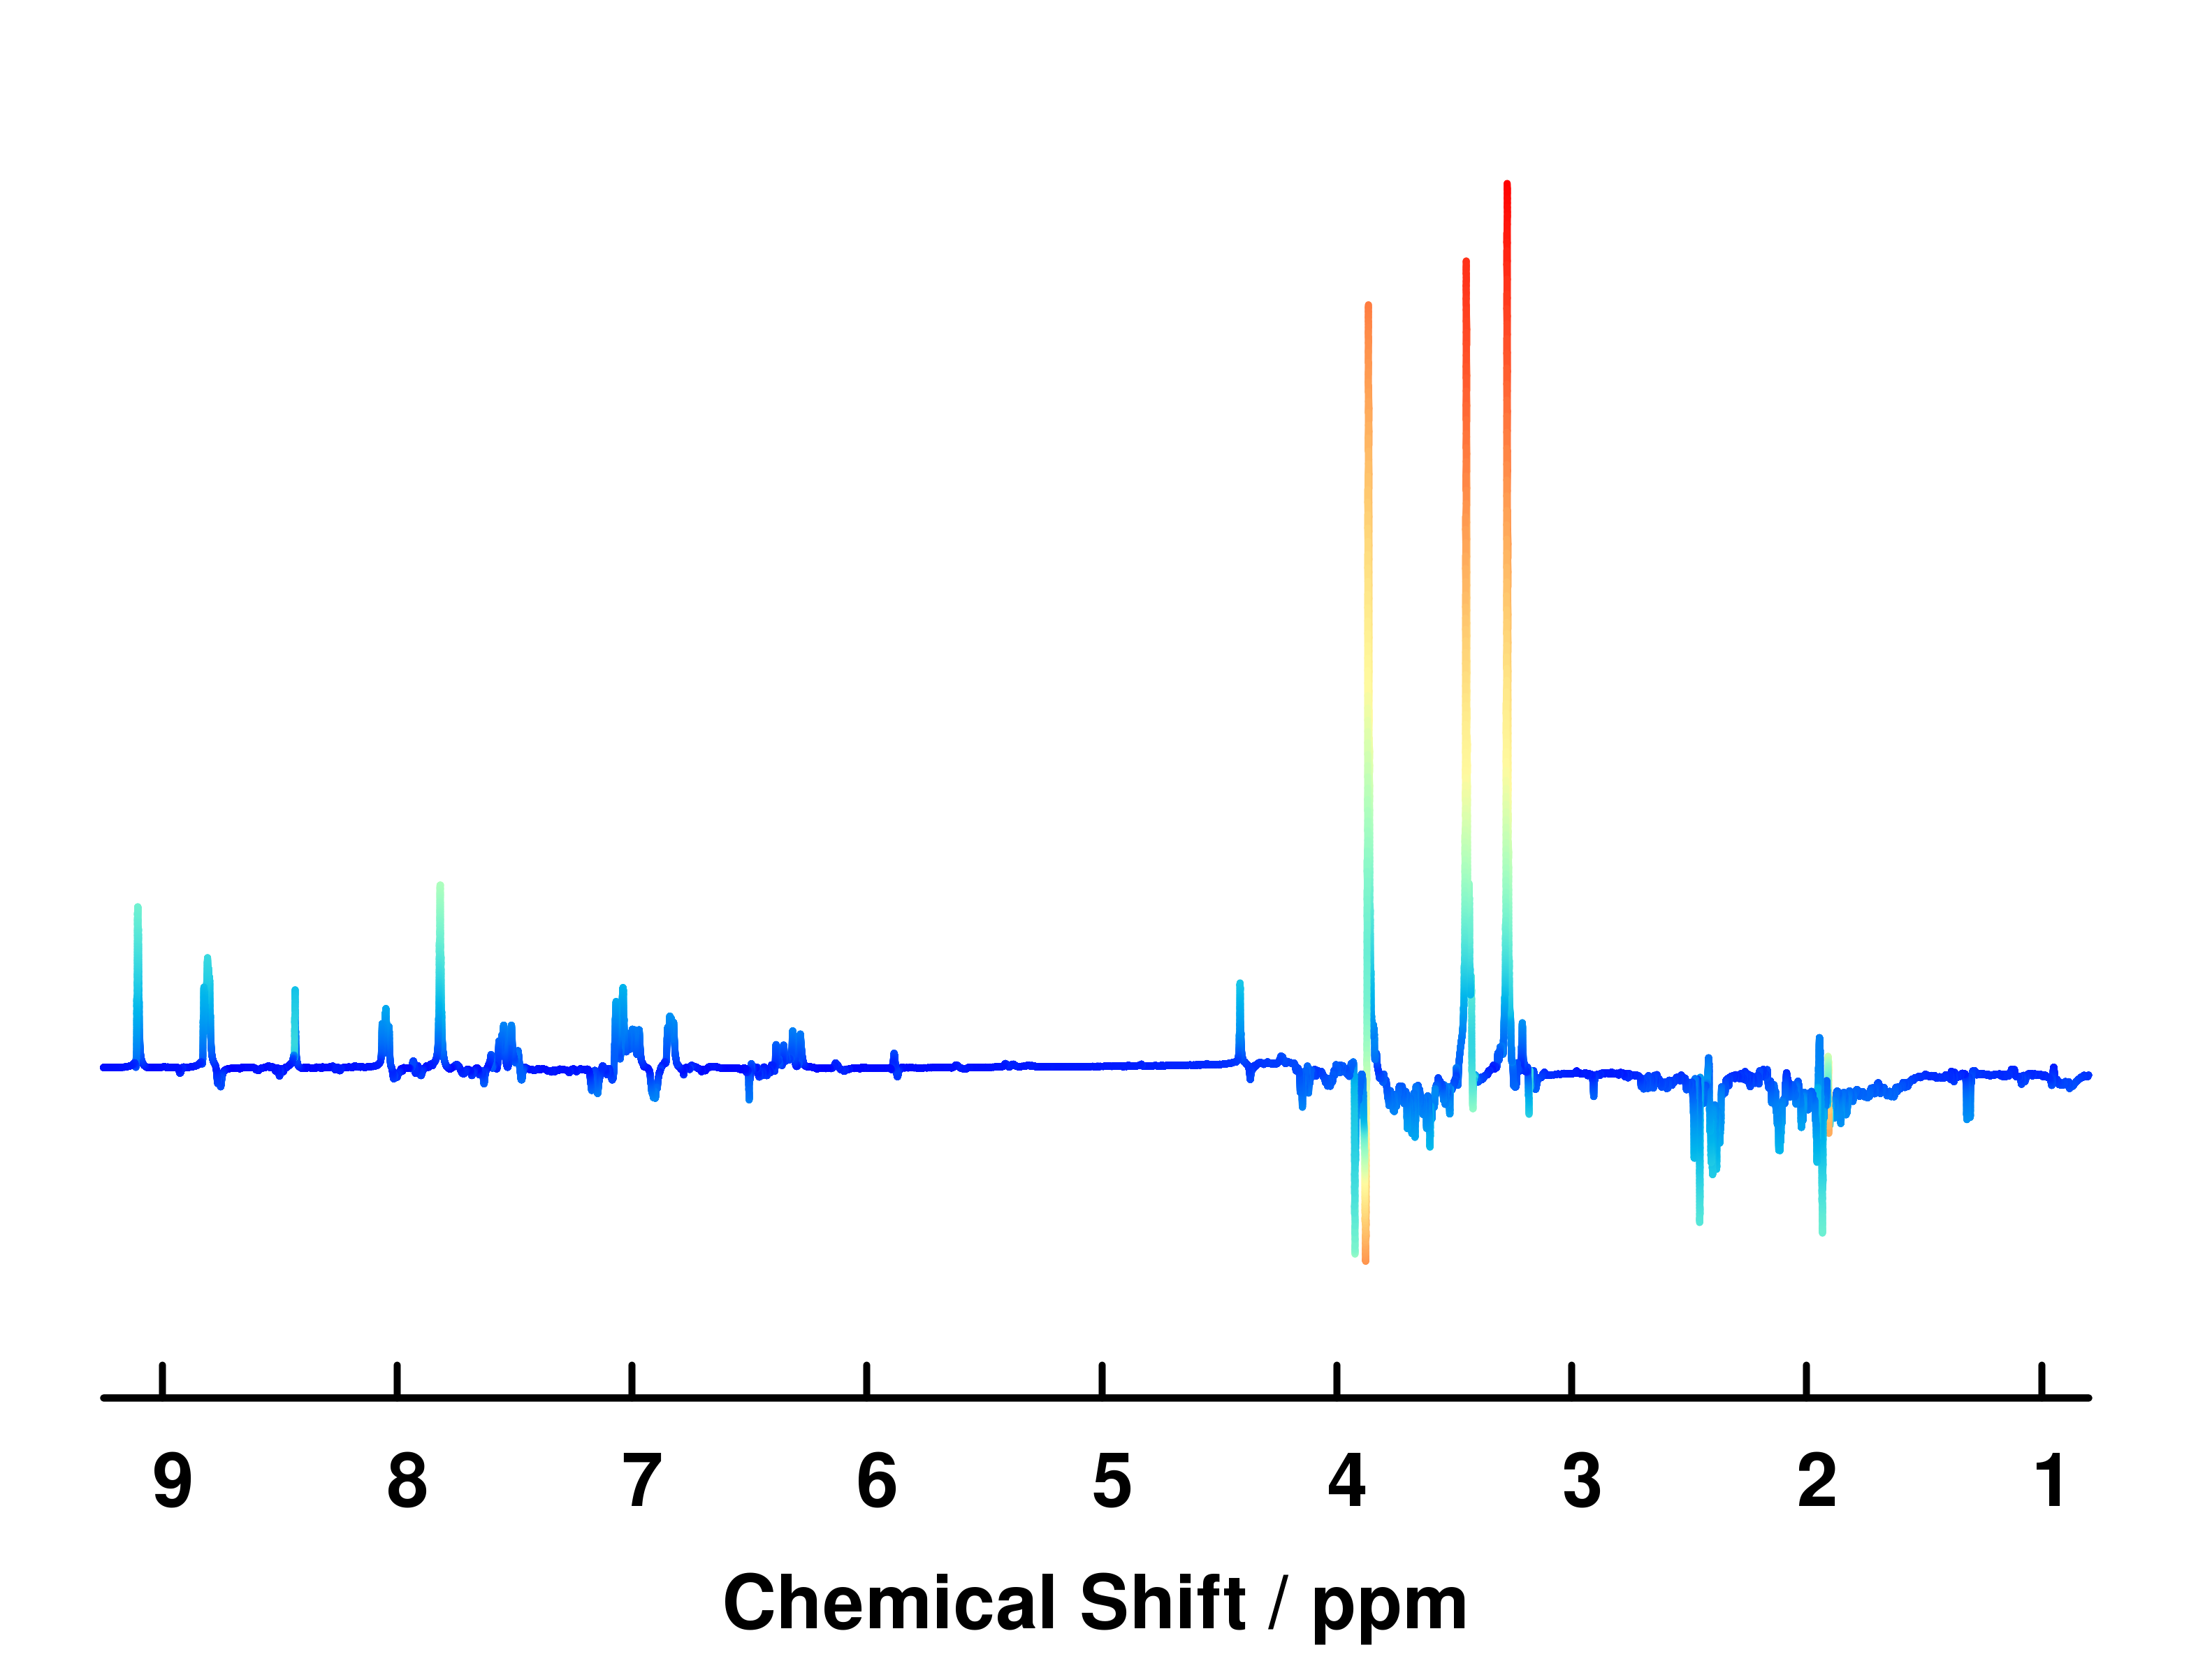
\includegraphics[width=3.5in]{figs/apps/04-oplsr-p.png}
\caption
      [Backscaled Coffees OPLS-R Model Loadings.]{
  {\bf Backscaled Coffees OPLS-R Model Loadings.}
  \\
  Backscaled OPLS-R predictive loadings of the four coffee roasts regressed
  according to estimated caffeine concentration. The pseudospectral nature of
  backscaled loadings facilitates analysis of model results by any
  spectroscopist. The four most intense positive positive peaks in the
  loadings pseudospectrum correspond directly to caffeine NMR resonances
  archived in the BMRB, indicating a fairly successful regression against
  caffeine concentration.
}
\end{SCfigure}

\subsection{Results and Discussion}

\begin{doublespace}
Use of MVAPACK during analysis of the coffees dataset arguably facilitated
rapid identification of ideal processing, treatment and modeling parameters
during data handling. Use of automatic phase correction, adaptive intelligent
binning, and PQ normalization yielded a dataset in which three principal
components were sufficient to fully separate all classes in scores space,
and subsequent LDA modeling resulted in complete class separation in only
two components (Figure 4.3).
\\\\
As opposed to the PCA modeling procedure, which utilized binned spectra,
OPLS-R model training was performed using full-resolution 1D \hnmr{} NMR
spectra in order to reap the interpretive advantages of full-resolution
backscaled loadings (Figure 4.4). The availability of \emph{i}COshift
alignment \cite{savorani:jmr2010} in MVAPACK effectively makes the modeling
of full-resolution NMR spectral data possible by correcting positional noise
\cite{aberg:abc2009} in the spectra that corrupts the bilinear nature of the
data. By regressing the NMR data against estimates of caffeine concentration
obtained by UV/Vis spectroscopy (Figure 4.1), a loading pseudo-spectrum of
caffeine was obtained that matched almost perfectly with spectral data
deposited in the Biological Magnetic Resonance Bank \cite{ulrich:nar2008}.
It is conceivable that spectral features coextracted with caffeine in the
loadings correspond to coffee bean metabolites lost alongside caffeine during
roasting or decaffeination.
\end{doublespace}

\begin{figure}[H]
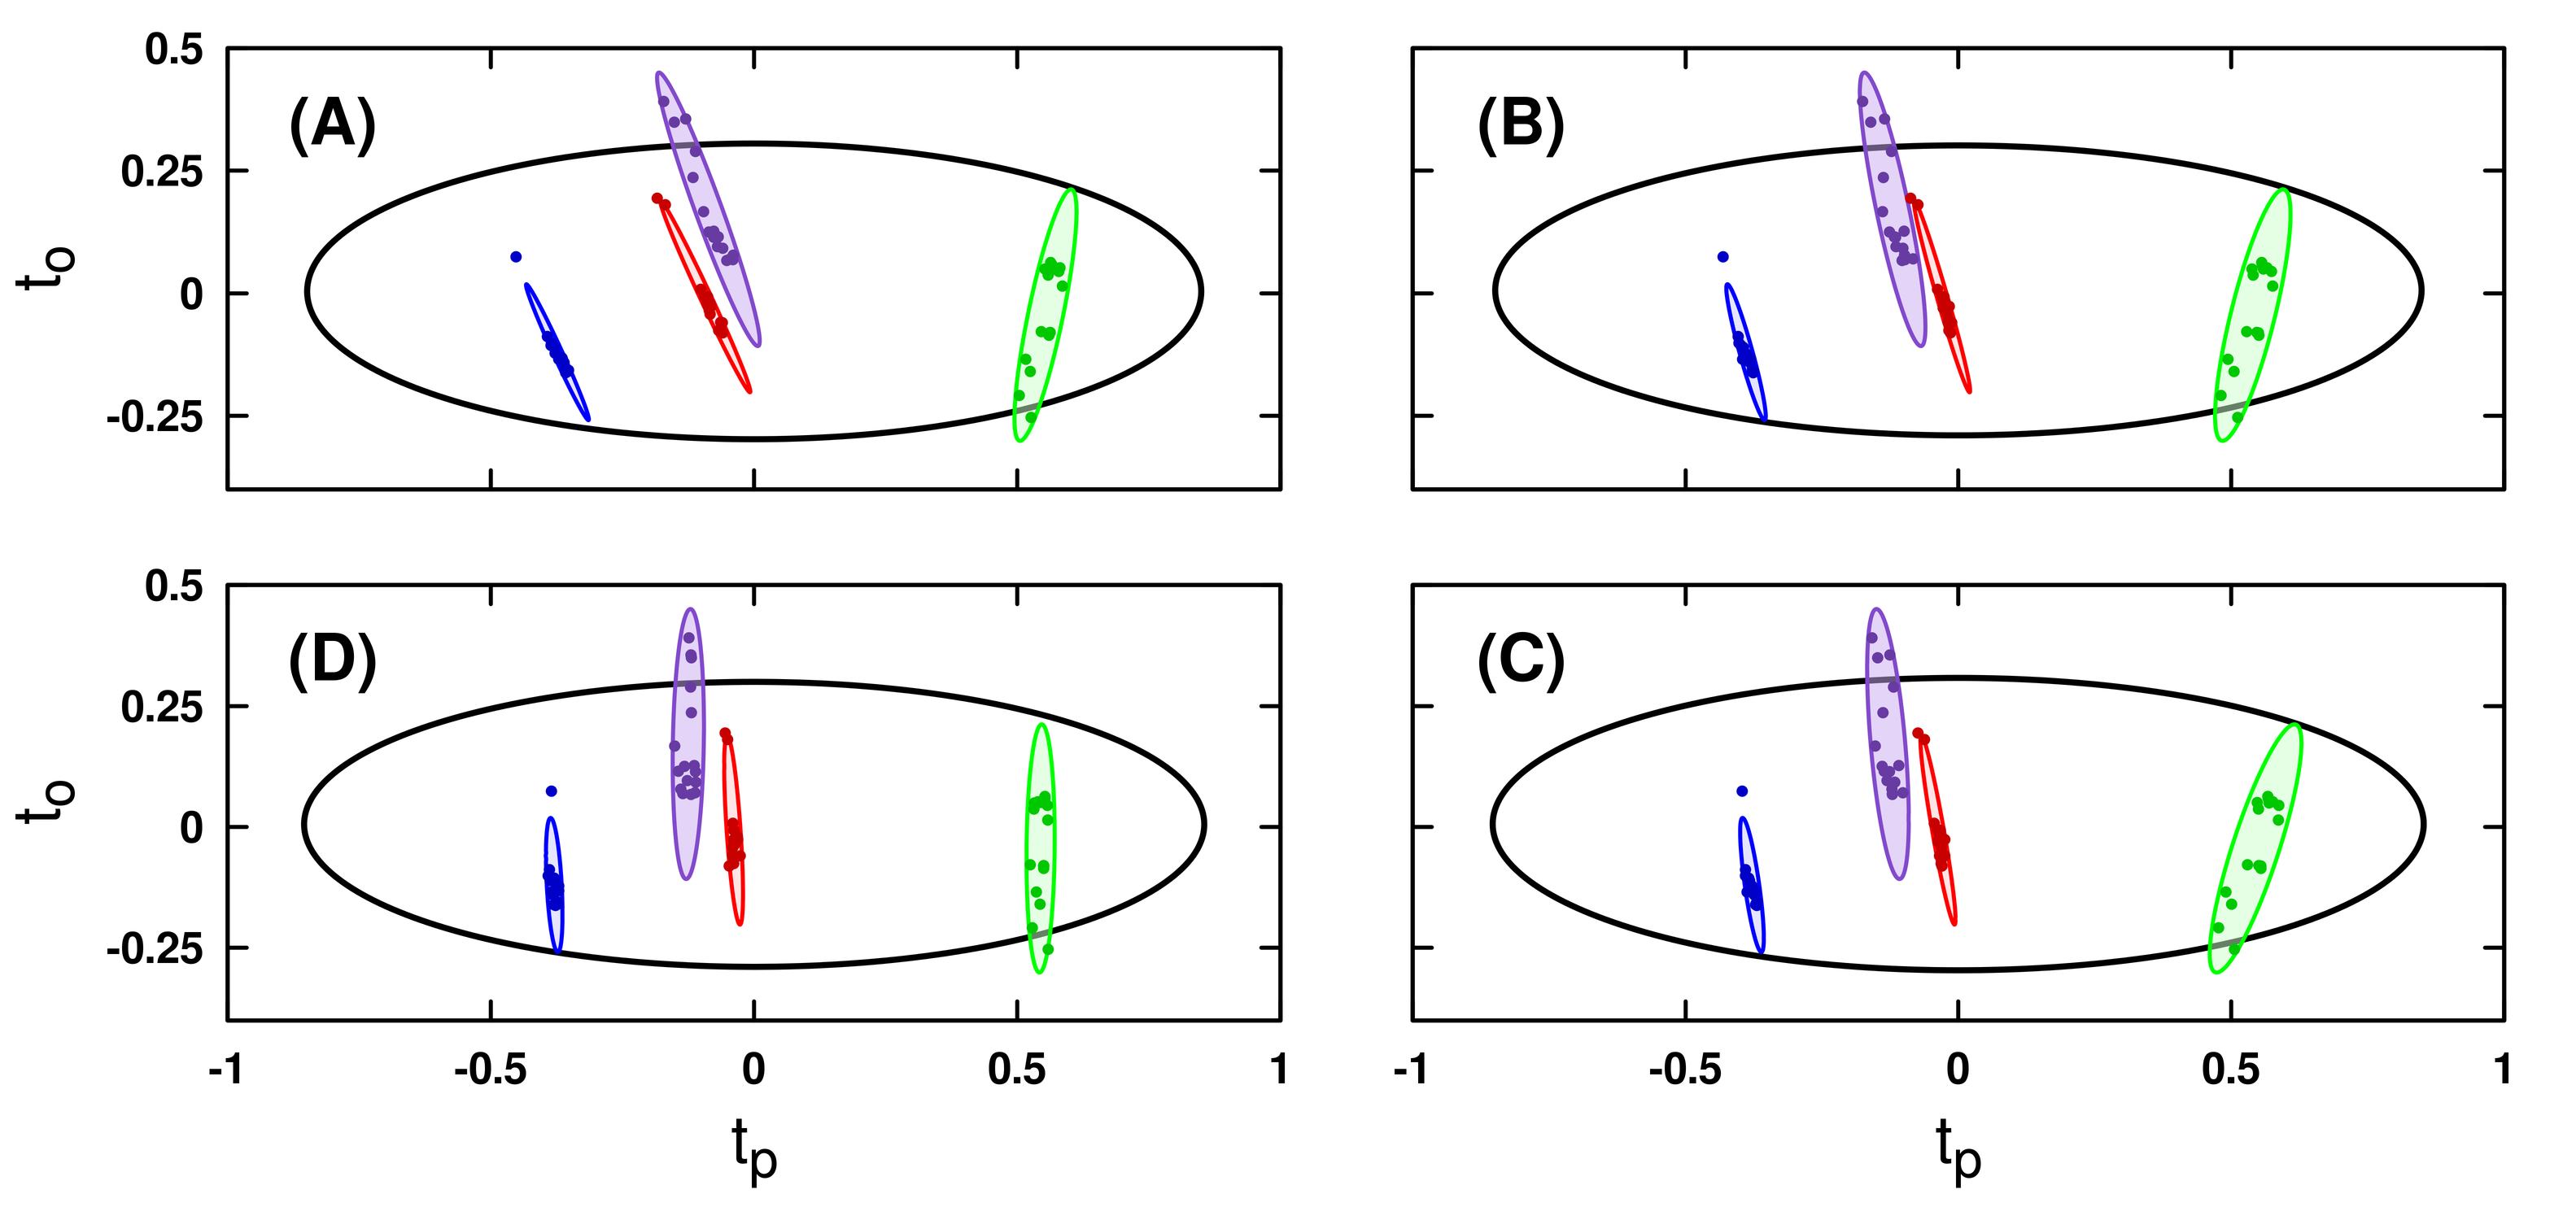
\includegraphics[width=6.5in]{figs/apps/05-oplsr-t.png}
\caption
      [Coffees OPLS-R Scores as Evidence of Overfit.]{
  {\bf Coffees OPLS-R Scores as Evidence of Overfit.}
  \\
  OPLS-R scores of the four coffee roasts, where each roast was regressed
  against its caffeine concentration estimated by UV/Vis absorbance
  spectroscopy. Scores in panels ({\bf A}) through ({\bf D}) were computed
  from models having 1 through 4 orthogonal components, respectively.
}
\end{figure}

\begin{figure}[H]
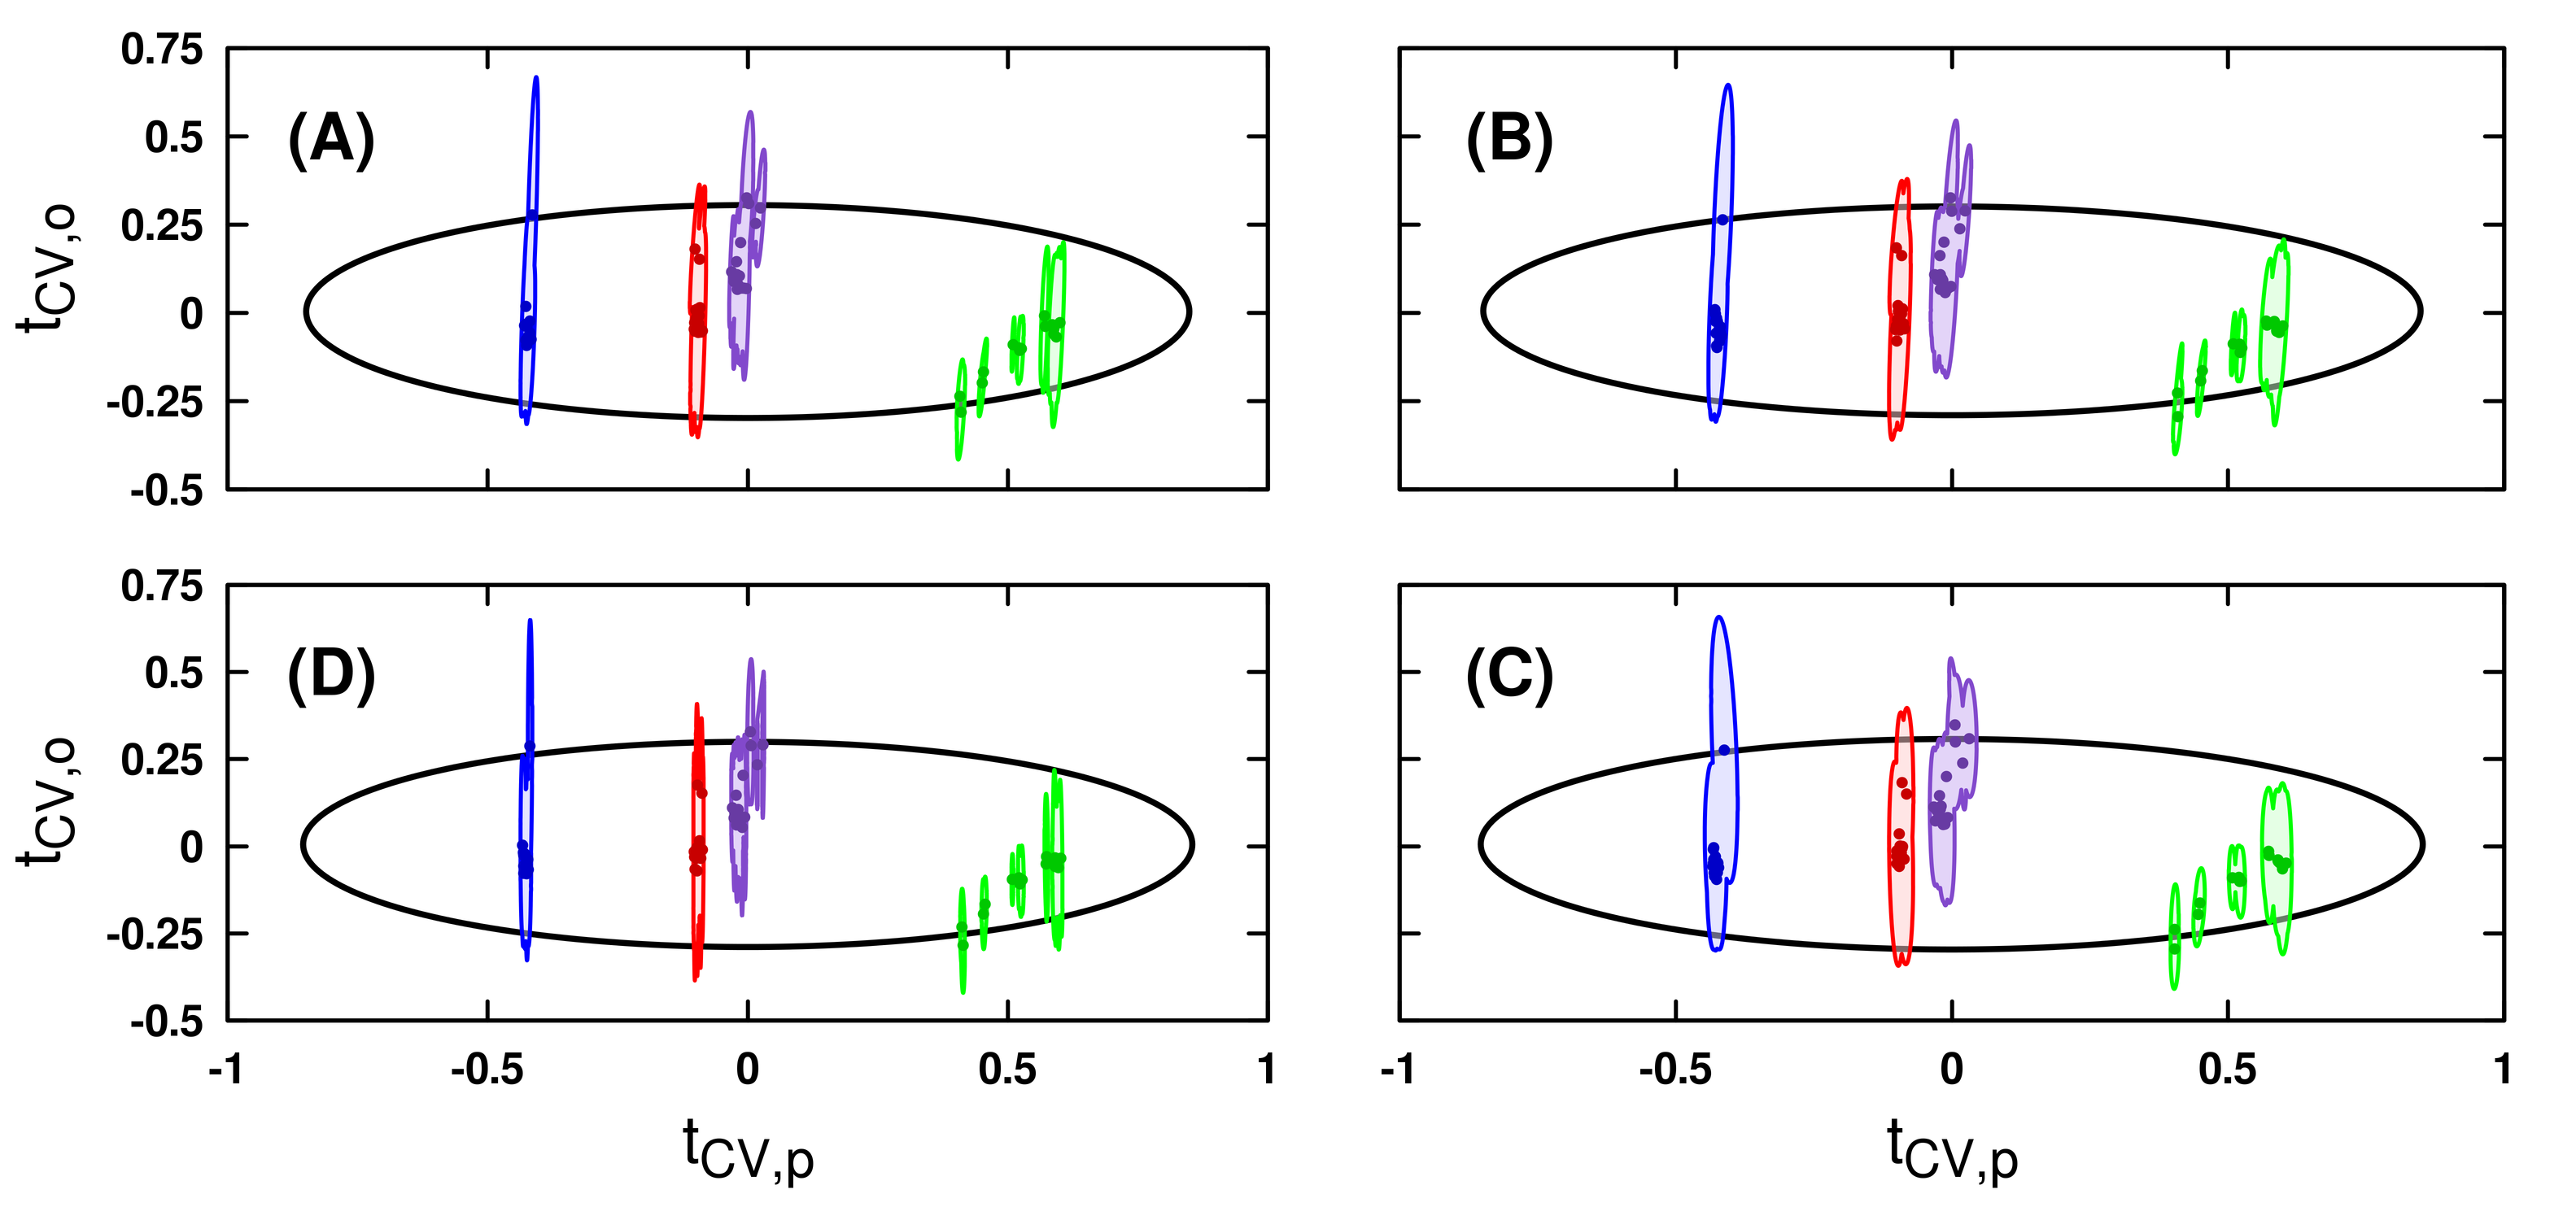
\includegraphics[width=6.5in]{figs/apps/06-oplsr-tcv.png}
\caption
      [Coffees OPLS-R Cross-validated Scores.]{
  {\bf Coffees OPLS-R Cross-validated Scores.}
  \\
  OPLS-R scores of the four coffee roasts, where each roast was regressed
  against its caffeine concentration, as in Figure 4.5. Mean score values
  and confidence ellipses for each observation were computed from 100
  iterations of seven-fold Monte Carlo internal cross-validation.
}
\end{figure}

\begin{doublespace}
Notably, the UV/Vis-estimated caffeine concentration of the dark roast coffee
was slightly higher than that of the medium roast, which is contrary to
expectation given that the coffees were brewed using equal volumes of
grounds. However, OPLS-R of the NMR data using the estimated caffeine
concentrations correctly ranked the roasts according to expectation
(Figure 4.5A). When more orthogonal components were allowed into the OPLS-R
model, the dark roast again shifted to a higher caffeine concentration,
beautifully indicating the presence of overfitting (Figure 4.5B--D).
Monte Carlo cross-validated scores further supported the fact that a $1+1$
OPLS model was the most appropriate (Figure 4.6). Therefore, an OPLS-R model
having only a single orthogonal component was chosen, given the fact that it
more faithfully modeled the underlying NMR data at the expense of
contradicting the more uncertain UV/Vis measurements.
\\\\
Finally, no discernable difference was observed between the 1D \hnmr{} NMR
spectra acquired with and without $T_2$-filtering. Spectra collected on
in-house brewed coffee exhibited high levels of protein background signal,
which were readily suppressed using the CPMG-$z$ pulse sequence element. On
the other hand, the spectra of the four purchased roasts showed no such
background signal, possibly due to more correct brewing technique.
\end{doublespace}

\section{Fingerprinting of Joint \hnmr{} NMR and DI-ESI-MS Data}

\begin{doublespace}
Multiblock bilinear factorizations such as CPCA, MB-PLS and MB-OPLS provide a
powerful framework for analyzing a set of multivariate observations from
multiple analytical measurements containing potentially correlated variables
\cite{westerhuis:jchemo1997,westerhuis:jchemo1998,smilde:jchemo2003}. Such
algorithms provide analogous information to PCA, PLS and OPLS in situations
where extra knowledge is available to subdivide the measured variables into
multiple ``blocks''. As a result, the correlation structures of each block
\emph{and} the between-block correlations may be simultaneously utilized.
Due to the existence of common trends among all blocks, this use of
between-block correlations during modeling will ideally bring the model
loadings (latent variables) into better agreement with the true underlying
biochemistry (hidden variables). In short, multiblock algorithms provide an
ideal means of integrating 1D \hnmr{} NMR and direct injection electrospray
mass spectrometry (DI-ESI-MS) datasets for metabolic fingerprinting
\cite{xu:abc2013}.
\\\\
Consensus PCA (\hyperlink{subsection.3.5.4}{CPCA-W}),
Multiblock PLS (\hyperlink{subsection.3.5.5}{MB-PLS}), and
Multiblock OPLS (\hyperlink{subsection.3.5.6}{MB-OPLS}) were used to analyze
1D \hnmr{} NMR and DI-ESI-MS data collected on metabolite extracts from
human dopaminergic neuroblastoma cells (SK-N-SH) after different neurotoxin
treatments \cite{marshall:metab2015}. Each dataset was also individually
subjected to single-block modeling by PCA and PLS in order to highlight the
information gained by jointly modeling the data within multiblock frameworks.
\end{doublespace}

\subsection{Materials and Methods}

\subsubsection{NMR Acquisition and Processing}

\begin{doublespace}
NMR data were collected and processed according to previously described
procedures \cite{zhang:jiomic2013}. A Bruker Avance DRX 500 MHz spectrometer
equipped with a 5 mm inverse triple-resonance cryoprobe (\hnmr{}, \cnmr{},
\nnmr{}) with a $z$-axis gradient, a BACS-120 sample changer, and an automatic
tuning and matching accessory were utilized for automated NMR data collection.
Free induction decays were collected into 32$k$ complex data points over a
spectral window of $2,342 \pm 2,741$ ppm, using the SOGGY water suppression
pulse sequence (\emph{zgesgp}, \cite{hwang:jmr1995,nguyen:jmr2007}).
\\\\
Following acquisition, the 1D \hnmr{} NMR free induction decays were processed
in the MVAPACK toolbox \cite{worley:acscb2014}. A 1.0 Hz exponential
apodization fuction and a single round of zero-filling were applied prior to
Fourier transformation. Spectra were then automatically phased and normalized
using phase-scatter correction (PSC, \cite{worley:cils2014},
cf. \hyperlink{chapter.6}{Chapter 6}). Finally, chemical shift regions
containing spectral baseline noise or solvent signals were manually removed.
Binning of the processed NMR spectra was performed using the Adaptive
Intelligent (AI) binning algorithm that avoids splitting signals into
multiple bins \cite{demeyer:anchem2008}.
\end{doublespace}

\subsubsection{MS Acquisition and Processing}

\begin{doublespace}
Mass spectra of the SK-N-SH metabolite extracts were acquired in positive ion
mode over a mass range of $m/z$ 50--1,200. Spectra were acquired for 30 s each
using the following source conditions: 2.5 kV electrospray capillary voltage,
60 V sampling cone voltage, 4.0 V extraction voltage, $80^\circ$C source
temperature, $250^\circ$C desolvation temperature, 500 L/h desolvation gas
flow rate, and 15 $\mu$L/min injection flow rate.
\\\\
The initial stages of mass spectral data processing were performed using
MassLynx V4.1 (Waters Corp., Milford, MA). A background subtraction was
performed on all spectra: reference spectra of either paraquat,
1-methyl-4-phenylpyridinium (MPP$^+$), rotenone, or 6-hydroxydopamine (6-OHDA)
in H$_2$O/CH$_3$OH/HCO$_2$H (49.75:49.75:0.5) at 10 ppm were used as
backgrounds. Background subtraction of each spectrum was performed in a
class-dependent manner (e.g. the MPP$^+$ reference mass spectrum was used as
background for MPP$^+$-treated cell samples). As a result, mass spectral
signals from the drugs themselves were guaranteed to not influence subsequent
analyses. The background-subtracted mass spectra were then loaded into MVAPACK
for binning and normalization. All mass spectra were linearly re-interpolated
onto a common axis that spanned from $m/z$ 50--1,200 in 0.003 $m/z$ steps,
resulting in 383,334 variables prior to processing. Based on the low
probability of observing a metabolite in the mass range $m/z$ 1,100--1,200,
the region was removed prior to binning. Mass spectra were uniformly binned
using a bin width of 0.5 $m/z$, resulting in a data matrix of 2,095 variables.
Finally, the MS data matrix observations were normalized using probabilistic
quotient (PQ) normalization \cite{dieterle:anchem2006}.
\end{doublespace}

\subsubsection{Multivariate Statistical Analysis}

\begin{doublespace}
Using functions available in the latest version of MVAPACK, the NMR and MS
data were joined into a single multiblock data structure and modeled using
CPCA-W, MB-PLS and MB-OPLS. Both blocks were scaled to unit variance prior
to modeling, and equal contribution of each block to the models (fairness)
was ensured by further scaling each block by the square root of its variable
count \cite{smilde:jchemo2003}. For the purposes of comparison, PCA and PLS
models of the independent NMR and MS data matrices were also constructed.
All PLS models were trained on a binary discriminant response matrix
(i.e. PLS-DA), in which untreated cells were assigned for one class,
and all neurotoxin-treated cells were assigned to a second class.
\end{doublespace}

\subsubsection{Cross-validation of Multivariate Models}

\begin{doublespace}
Initially, all PCA and CPCA-W models were internally cross-validated using a
leave-one-out (LOOCV) procedure in MVAPACK during model training
\cite{eshghi:cils2014}. A subsequent set of PCA models was trained and
cross-validated using a Monte Carlo seven-fold (MCCV) procedure that
produced less optimistic \qsq{} statistics. All PLS-DA, MB-PLS-DA and
MB-OPLS-DA models were internally cross-validated using a Monte Carlo
seven-fold procedure \cite{wold:cils2001}. All MCCV rounds involved 50
iterations per tested model component. The results of cross-validation
were summarized by per-component \qsq{} statistics, and the number of model
components was chosen such that the cumulative \qsq{} was a strictly increasing
function of component count. Response permutation tests of all supervised
models were performed with 1,000 permutations each to assess the statistical
significance of \rsqy{} and \qsq{} values \cite{westerhuis:metab2008a}.
CV-ANOVA significance tests \cite{eriksson:jchemo2008} were also performed
to supplement the results of the permutation tests.
\end{doublespace}

\begin{SCfigure}
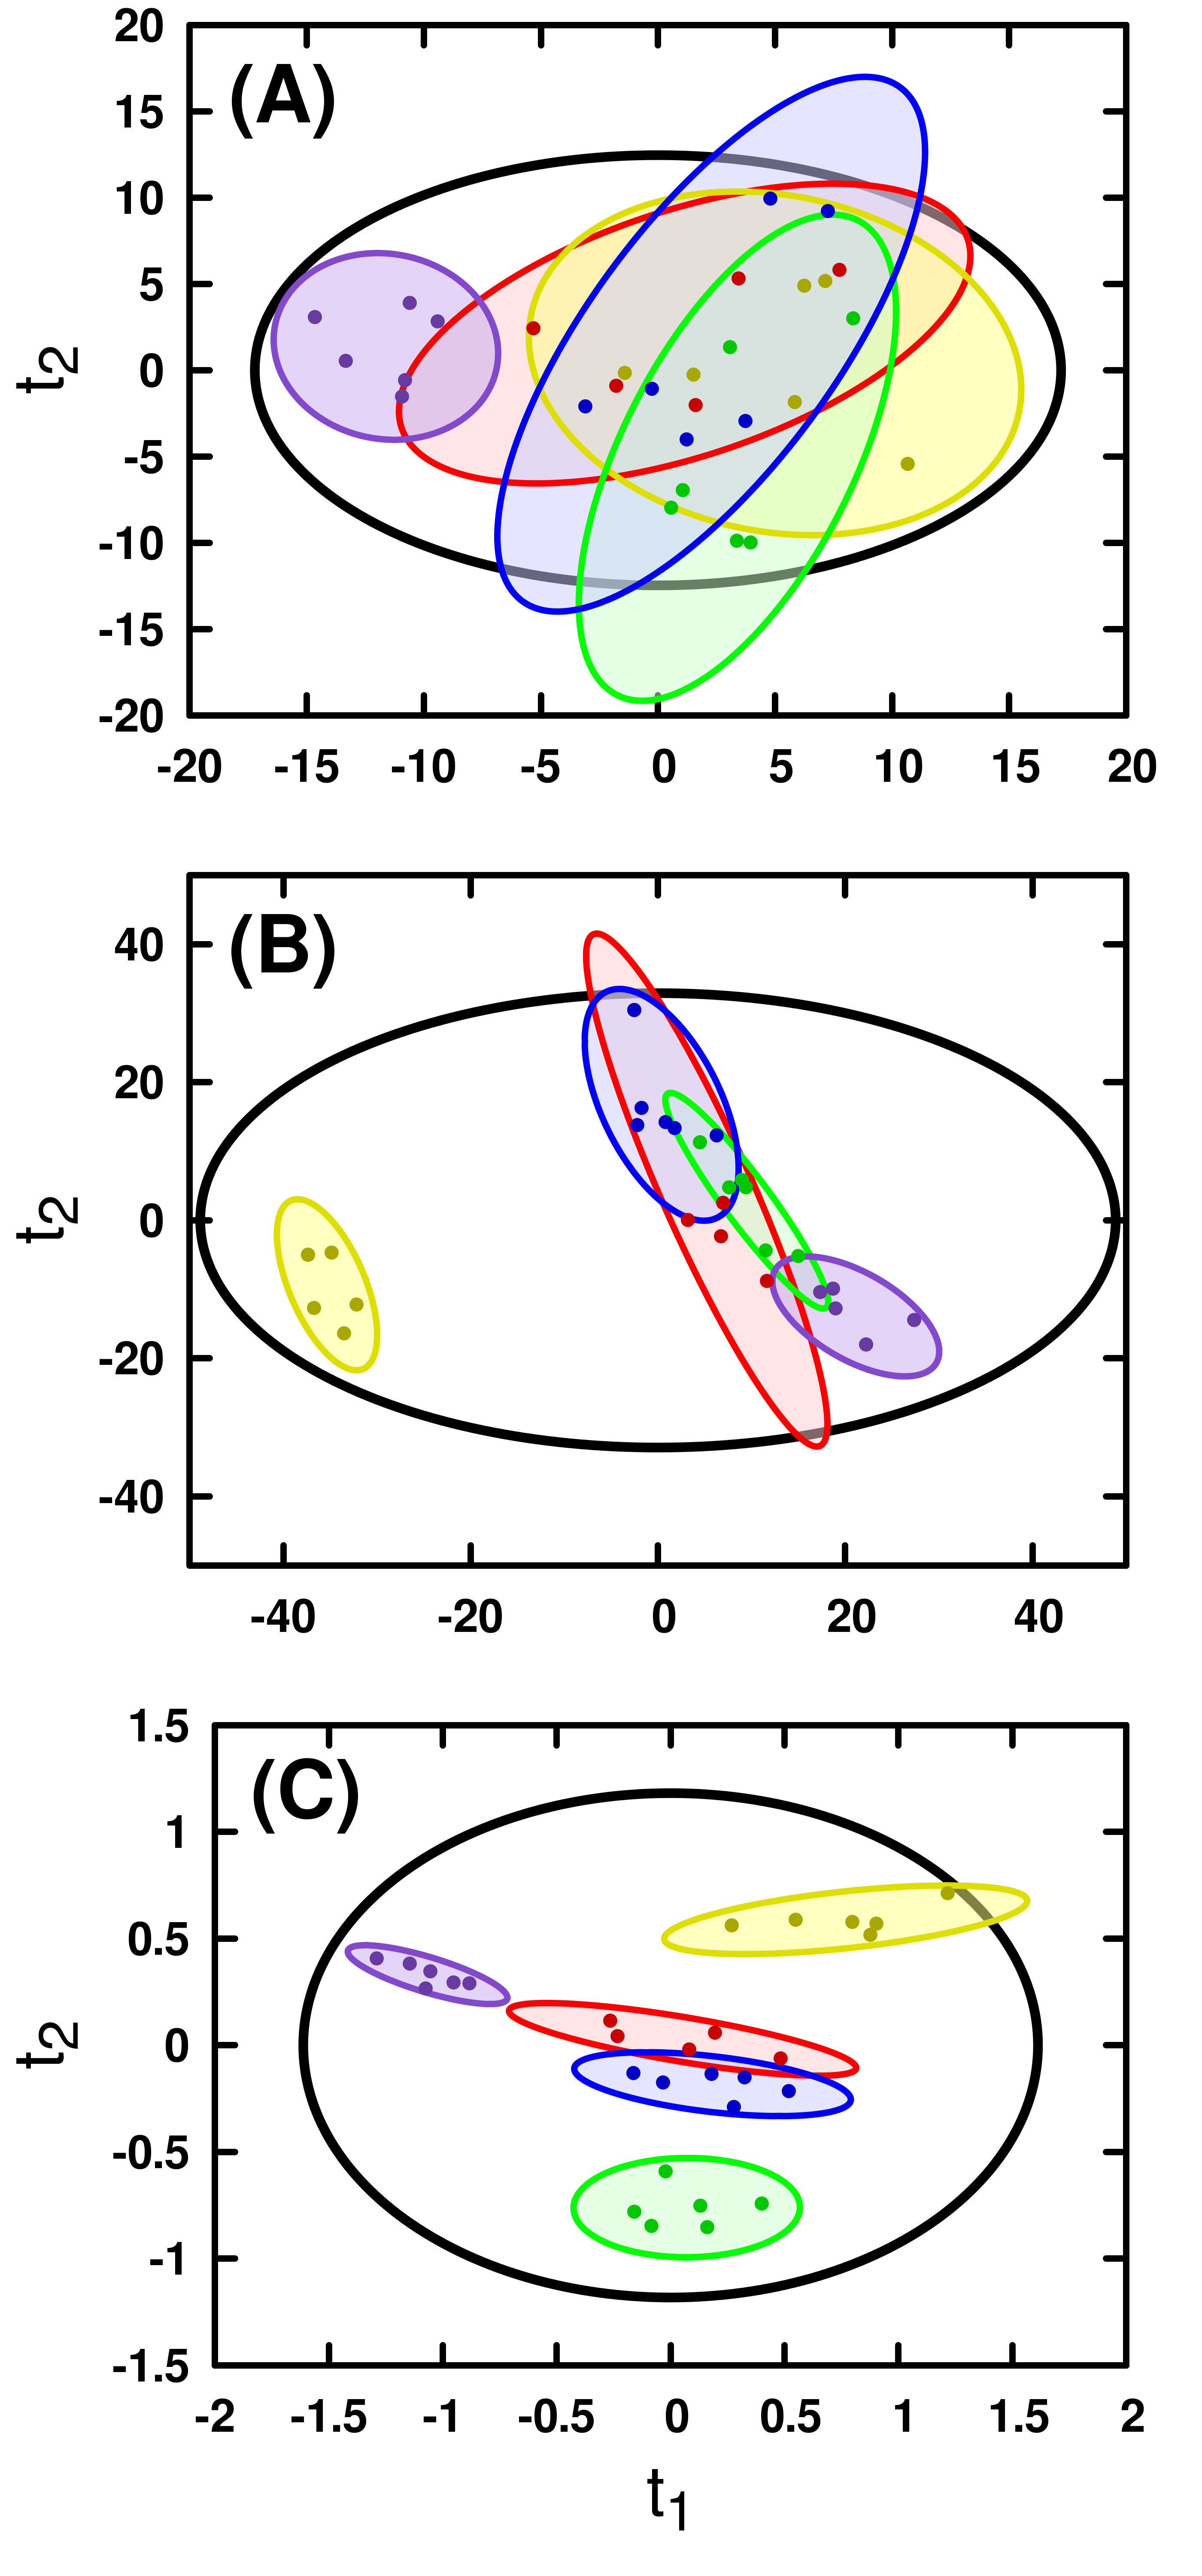
\includegraphics[width=3.5in]{figs/apps/07-mbpca-t.png}
\caption
      [Comparison of PCA and MB-PCA Scores.]{
  {\bf Comparison of PCA and MB-PCA Scores.}
  \\
  Scores generated from ({\bf A}) PCA of \hnmr{} NMR in vacuo, ({\bf B}) PCA
  of DI-ESI-MS in vacuo, and ({\bf C}) MB-PCA of \hnmr{} NMR and DI-ESI-MS.
  Separations between classes are increased upon combination of the two
  data matrices via MB-PCA. Yellow, red, green, violet and blue scores
  correspond to the control, 6-OHDA, MPP$^+$, paraquat and rotenone classes,
  respectively.
}
\end{SCfigure}

\begin{SCfigure}
\includegraphics[width=2.5in]{figs/apps/08-mbpca-d.png}
\caption
      [Dendrograms of PCA and MB-PCA Scores.]{
  {\bf Dendrograms of PCA and MB-PCA Scores.}
  \\
  Dendrograms computed from scores-space class separations
  \cite{worley:abio2013} in the in vacuo PCA and MB-PCA models. Panels
  ({\bf A--C}) correspond to scores in panels ({\bf A--C}) in Figure 4.7,
  above.
}
\end{SCfigure}

\subsection{Results and Discussion}

\subsubsection{Classical Modeling}

\begin{doublespace}
PCA of the binned NMR data matrix ($N = 29, K = 159$) resulted in 10 principal
components having cumulative \rsqx{} and \qsq{} statistics of 0.9485 and
0.4591, respectively, based on LOOCV. Overall, no patterns were readily
discernable in the NMR PCA scores (Figure 4.7A) due to high within-class
variation in the data. However, scores for paraquat treatment were found
to significantly separate from all other classes ($p < 0.002$) along the
first principal component. Scores from PCA of the binned MS data matrix
($N = 29, K = 2,095$) were found to exhibit markedly less within-class
variation compared to the NMR data (Figure 4.7B). Using LOOCV, three
significant components were identified from the binned MS data, yielding
fairly low cumulative \rsqx{} and \qsq{} statistics of 0.3397 and 0.1590.
While paraquat treatment still separated from other drug treatments in MS
PCA scores space, the greatest separations were observed between treated
and untreated (control) cells ($p < 1.0 \times 10^{-9}$). These differing
patterns of separation in NMR and MS PCA scores suggested that multiblock
analyses could provide further information, ideally separating both control
and paraquat scores from all other classes. Figure 4.8 contains dendrograms
of scores-space class separation for each scores plot in Figure 4.7.
\\\\
Per-component \qsq{} statistics computed from LOOCV of the NMR and MS PCA
models suggested fairly marginal model reliability at component counts greater
than one, so follow-up analyses were performed using MCCV on the same data
matrices to obtain less optimistic estimates of reliability. In both cases,
MCCV produced single-component PCA models, indicating that the LOOCV had
substantially over-estimated the number of principal components in each
matrix. A comparison of the resulting \qsq{} statistics from LOOCV and MCCV
is shown in Figure 4.9.
\\\\
PLS-DA of the full-resolution NMR ($N = 29, K = 16,138$) and
MS ($N = 29, K = 2,095$) data matrices both resulted in two-component models.
With the exception of the algorithmically forced separation between control
and treatment classes, similar clustering patterns were observed when compared
to the PCA scores (cf. Figure 4.10A--B). MCCV results from the
NMR ($R^2_Y = 0.9519, Q^2 = 0.7303 \pm 0.0517$) and
MS ($R^2_Y = 0.9951, Q^2 = 0.9440 \pm 0.01142$) PLS-DA models indicated
reasonable levels of response fit and predictive ability. Further validation
by CV-ANOVA \cite{eriksson:jchemo2008} indicated reliable models with $p$
values of 0.002 and $9.8 \times 10^{-6}$ for NMR and MS data, respectively.
Response permutation tests for both PLS-DA models returned $p < 0.001$,
supporting the CV-ANOVA test results.
\end{doublespace}

\begin{SCfigure}
\includegraphics[width=3.5in]{figs/apps/09-rqpca.png}
\caption
      [Comparison of LOOCV and MCCV \qsq{} Statistics for PCA.]{
  {\bf Comparison of LOOCV and MCCV \qsq{} Statistics for PCA.}
  \\
  \rsq{} (red), $Q^2_{\mathrm{LOOCV}}$ (green) and $Q^2_{\mathrm{MCCV}}$ (blue)
  statistics from ({\bf A}) PCA of \hnmr{} NMR in vacuo, ({\bf B}) PCA of
  DI-ESI-MS in vacuo, and ({\bf C}) MB-PCA of \hnmr{} NMR and DI-ESI-MS.
  In all cases, MCCV indicates that both datasets contain a single significant
  principal component, while LOOCV over-estimates the number of significant
  components.
}
\end{SCfigure}

\begin{SCfigure}
\includegraphics[width=3.5in]{figs/apps/10-mbpls-t.png}
\caption
      [Comparison of PLS-DA and MB-PLS-DA Scores.]{
  {\bf Comparison of PLS-DA and MB-PLS-DA Scores.}
  \\
  Cross-validated scores generated from ({\bf A}) PLS-DA of \hnmr{} NMR in
  vacuo, ({\bf B}) PLS-DA of DI-ESI-MS in vacuo, and ({\bf C}) MB-PLS-DA of
  \hnmr{} NMR and DI-ESI-MS. Consensus directions in MB-PLS-DA scores space
  show decreased rotation during cross-validation when compared to PLS-DA
  scores of the in vacuo PCA model. Yellow, red, green, violet and blue scores
  correspond to the control, 6-OHDA, MPP$^+$, paraquat and rotenone classes,
  respectively.
}
\end{SCfigure}

\subsubsection{Multiblock Modeling}

\begin{doublespace}
Identification of consensus directions in the NMR and MS data matrices that
maximally captured overall variation (MB-PCA) or response correlations (MB-PLS)
resulted in more informative models than those calculated against either NMR
or MS in vacuo. Using MB-PCA with LOOCV, five significant components were
identified ($Q^2 = 0.2322$) that cumulatively explained comparable amounts
of variation in the NMR ($R^2_X = 0.8528$) and MS ($R^2_X = 0.5015$) blocks
relative to the individual PCA models. As expected, MB-PCA combined the
information from both blocks to dramatically increase class separations in
super-scores space (Figure 4.7C). More specifically, both control and paraquat
classes were separated from other neurotoxin treatments, predominantly along
the first principal component. Furthermore, MPP$^+$ treatment exhibited
significant separation from 6-OHDA and rotenone treatments, which was not
expected from examination of the individual NMR or MS PCA scores.
\end{doublespace}

\begin{figure}[ht!]
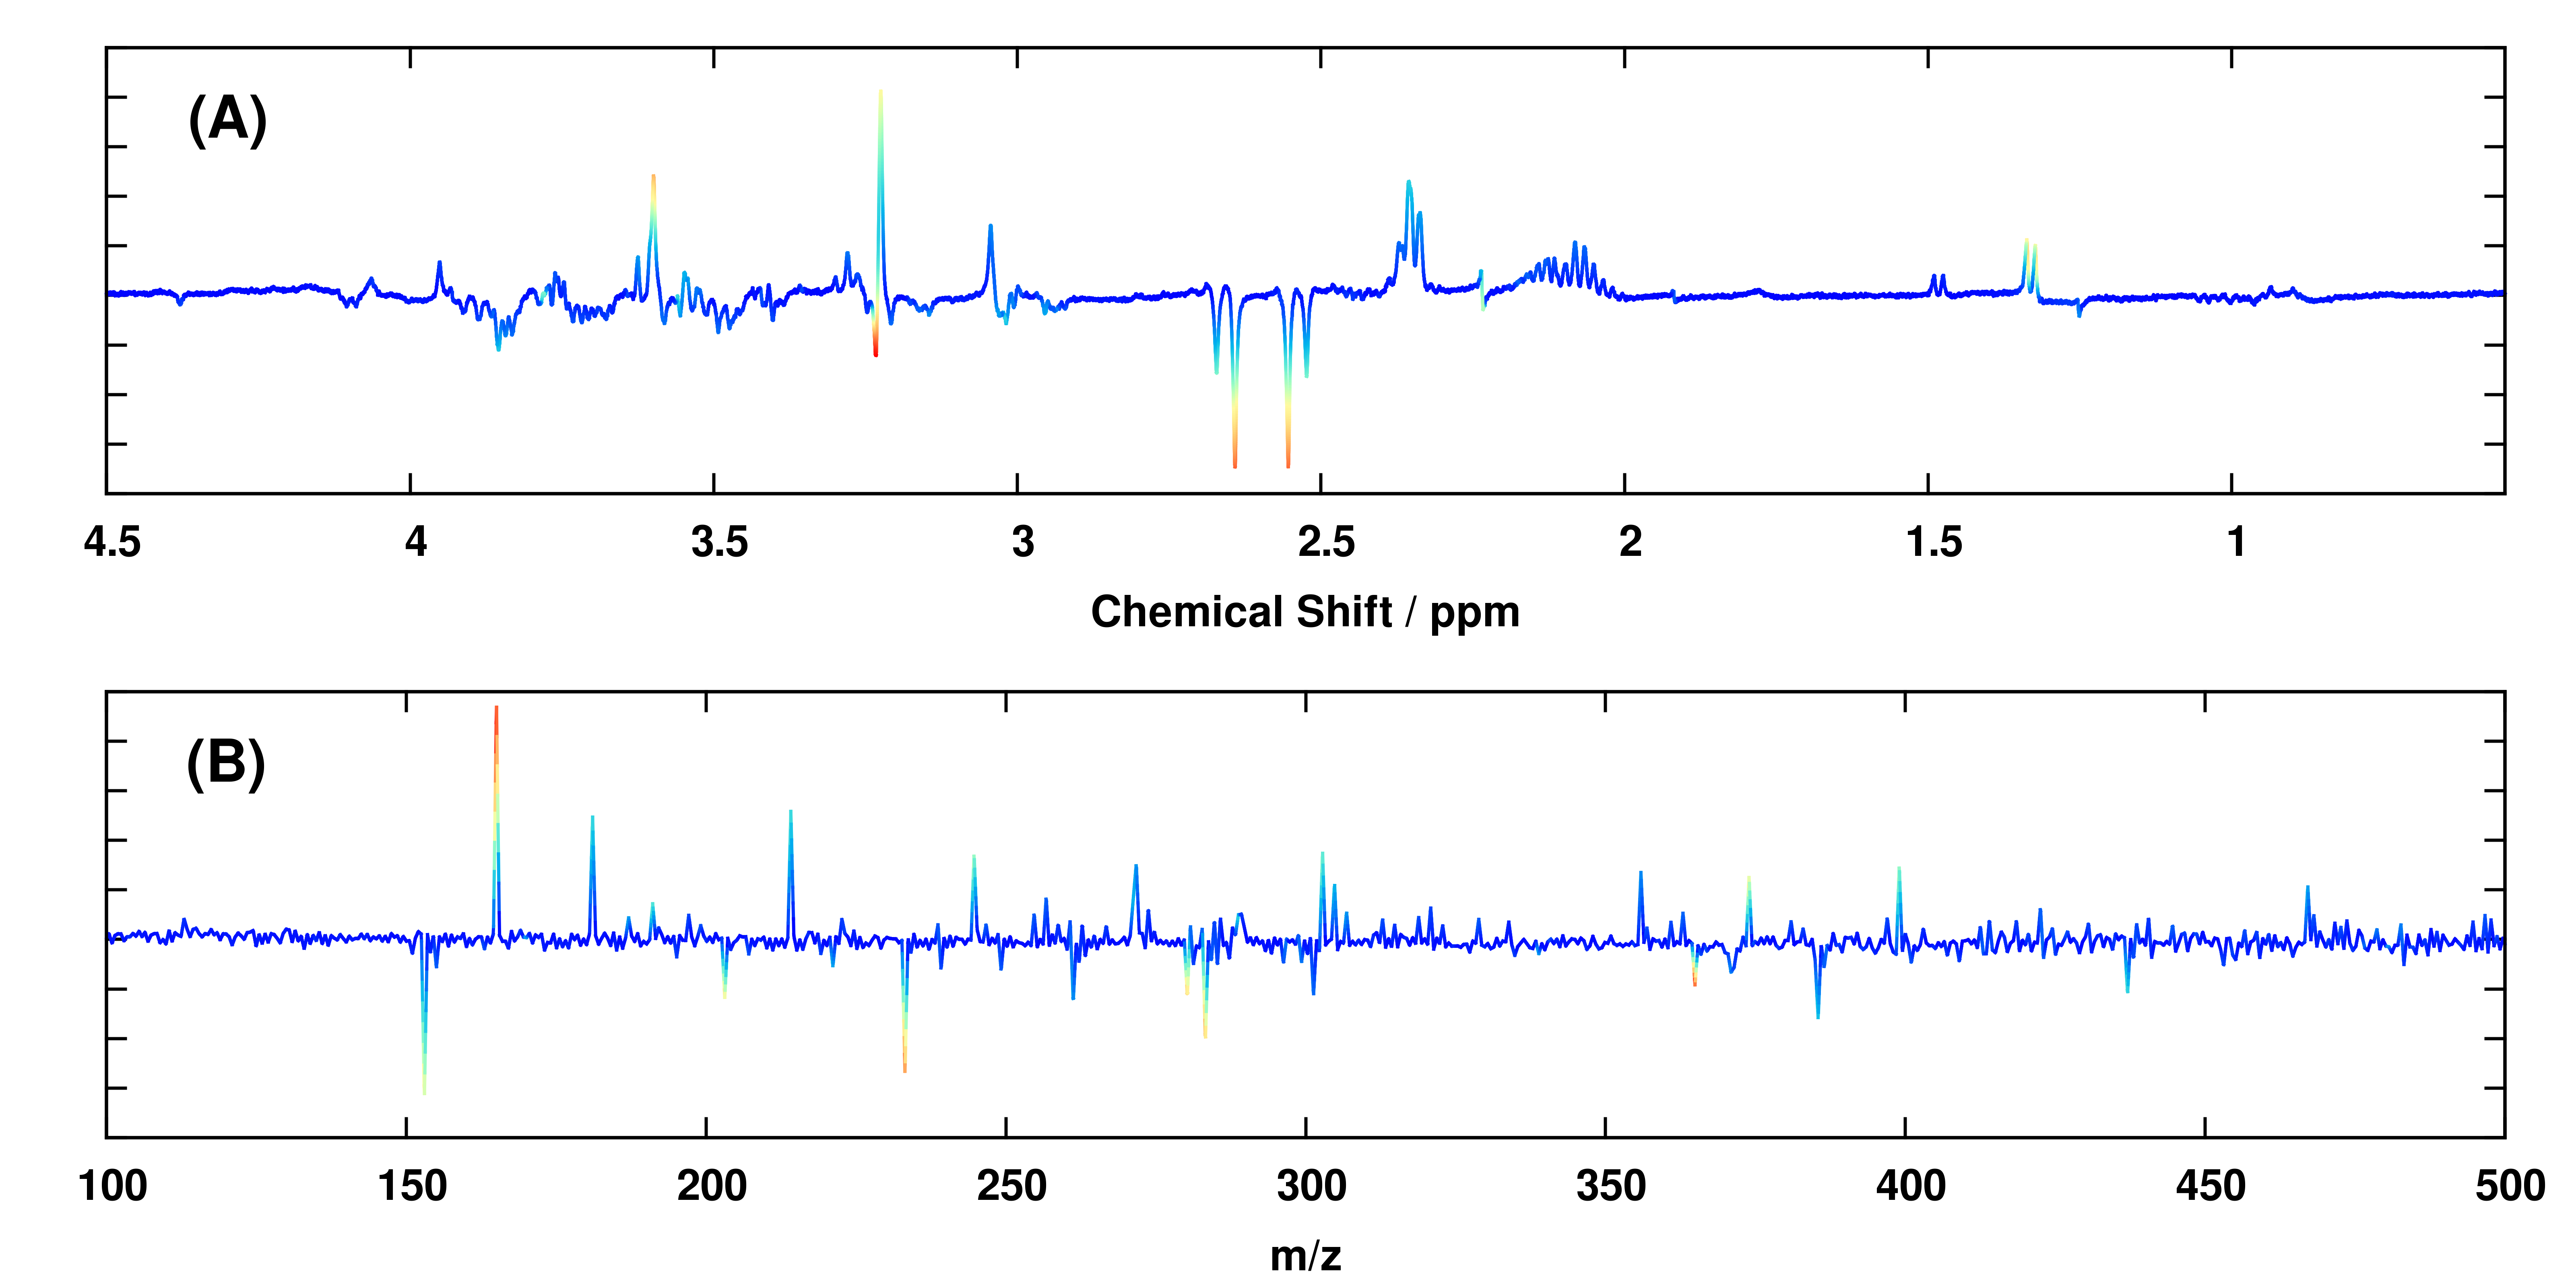
\includegraphics[width=6.5in]{figs/apps/11-mbpls-p.png}
\caption
      [Backscaled NMR and MS Block Loadings.]{
  {\bf Backscaled NMR and MS Block Loadings.}
  \\
  Backscaled ({\bf A}) \hnmr{} NMR block and ({\bf B}) DI-ESI-MS block loadings
  from MB-PLS-DA. Comparison of the above panels to those from MB-OPLS-DA
  (Figures 4.12, 4.13) reveals the mixed predictive and orthogonal variation
  present in MB-PLS loadings. It is also important to note that a second
  PLS component exists, and thus complete interpretation of the joint NMR
  and MS data requires simultaneous examination of \emph{two} sets of
  block loadings.
}
\end{figure}

\begin{doublespace}
Subsequent re-evaluation of the MB-PCA model's reliability using MCCV reduced
the number of expected significant components to two (Figure 4.9C). However,
secondary and higher components' \qsq{} statistics were still found to be
statistically indistinguishable from zero, which further suggests that only
one principal direction exists in the binned NMR and MS data matrices that
captures any substantial variation.
\end{doublespace}

\begin{figure}[ht!]
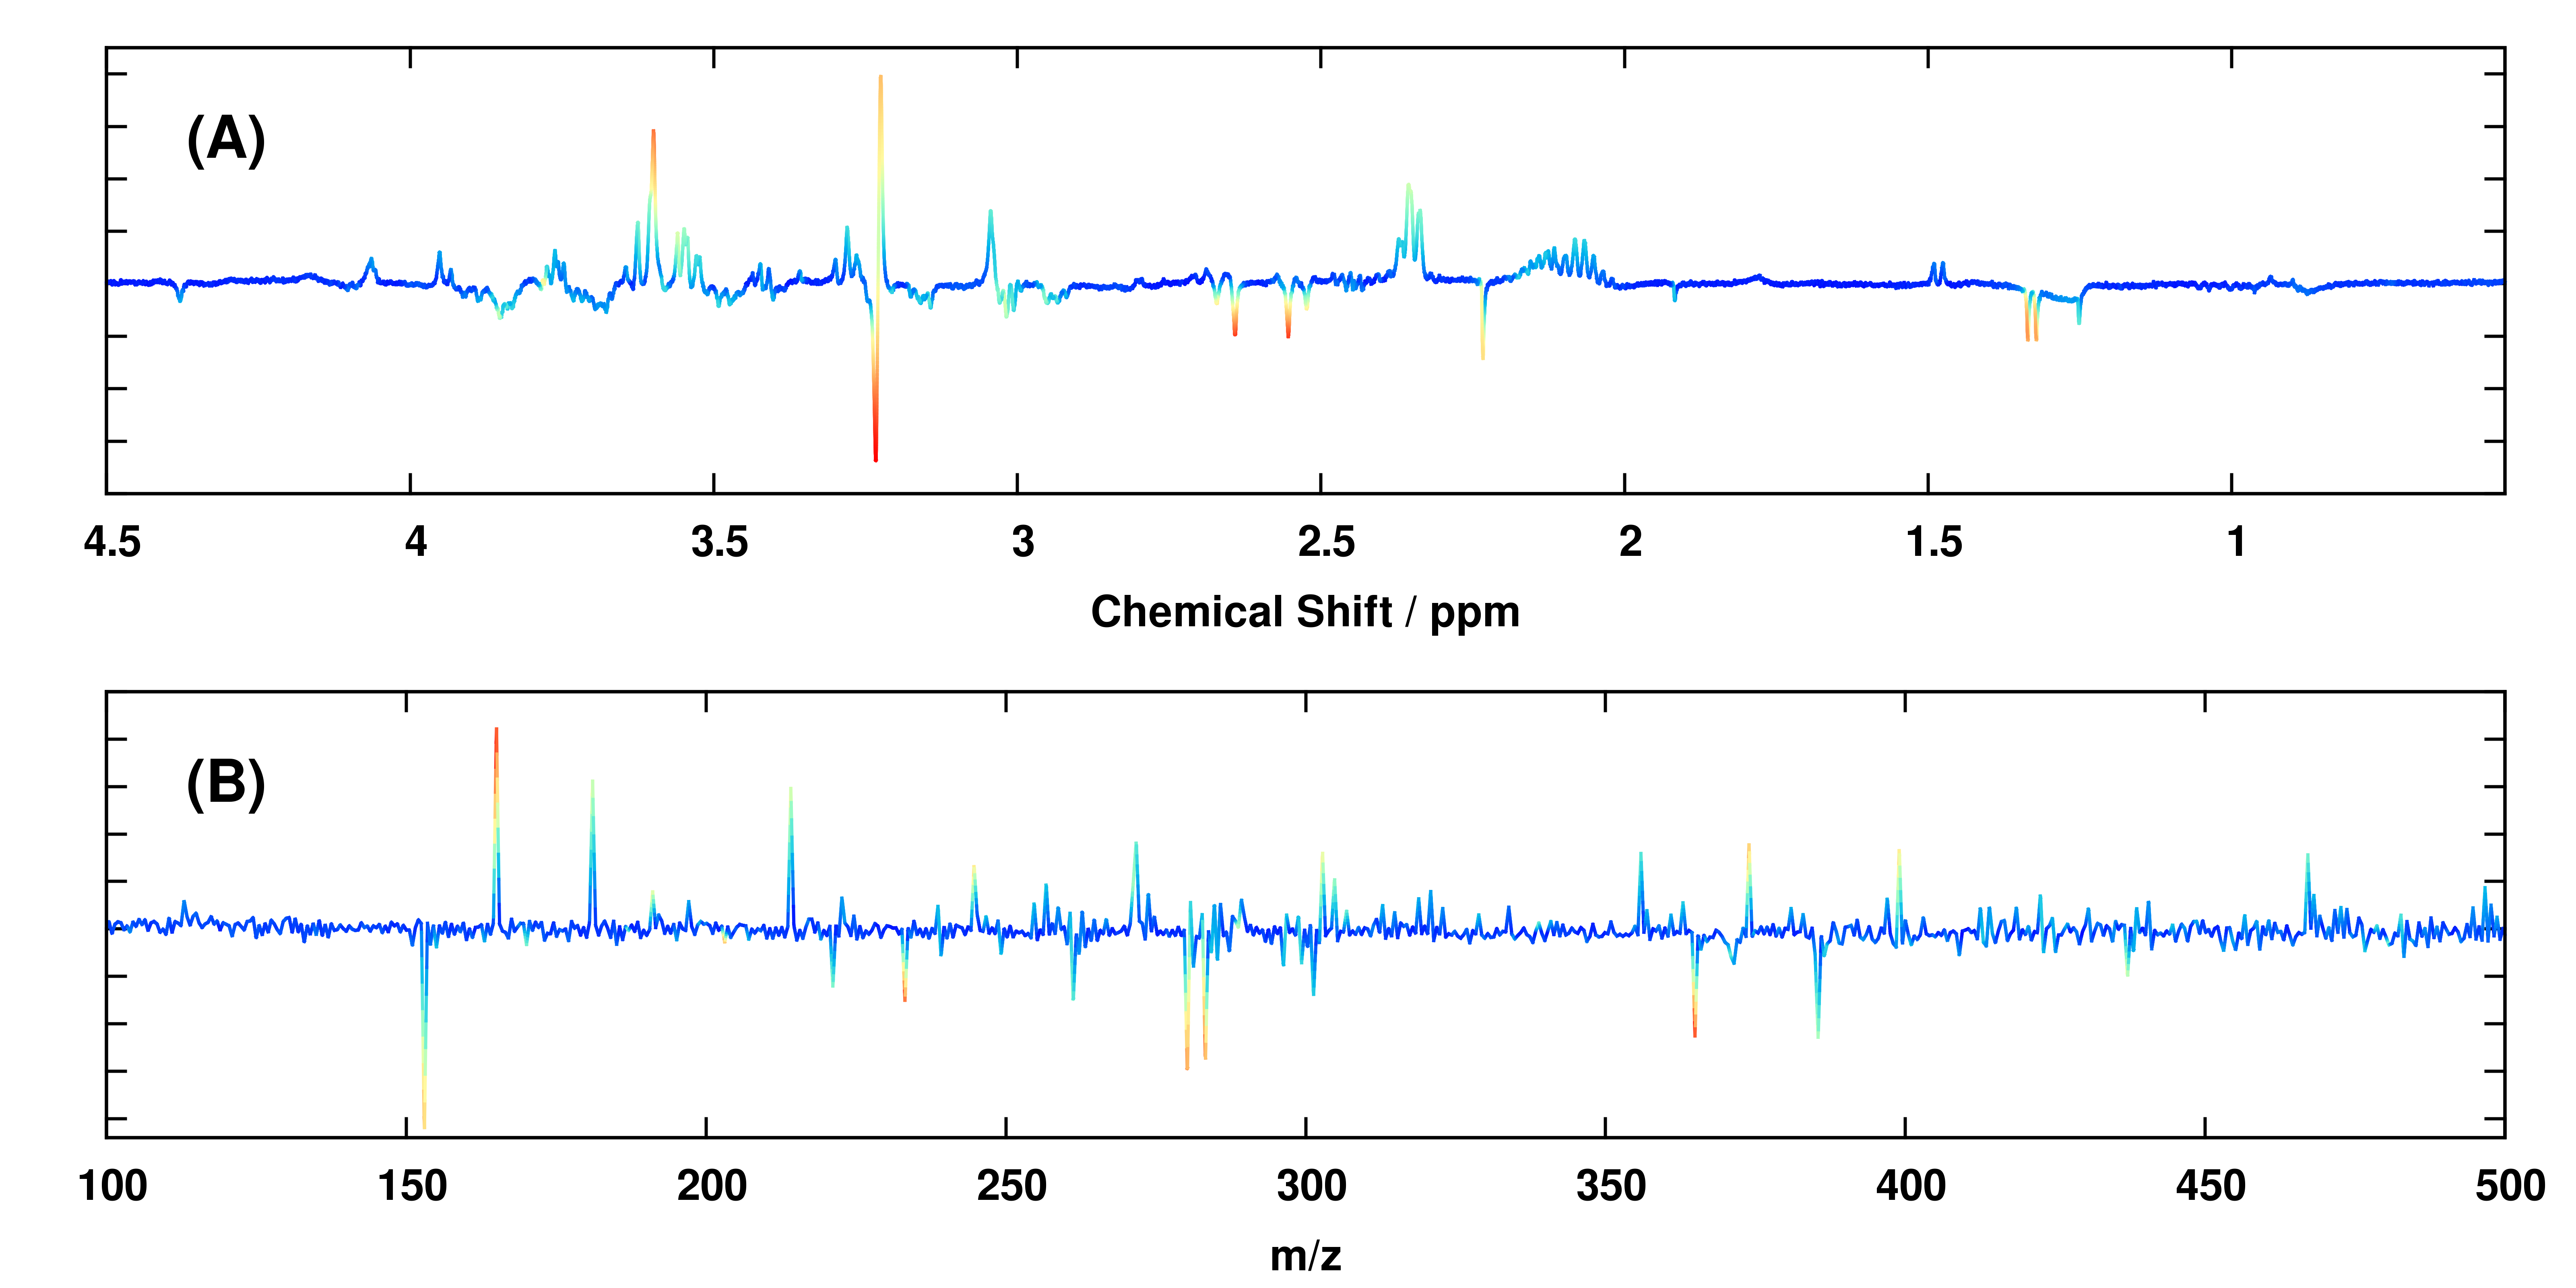
\includegraphics[width=6.5in]{figs/apps/12-mbopls-p.png}
\caption
      [Backscaled NMR and MS Predictive Block Loadings.]{
  {\bf Backscaled NMR and MS Predictive Block Loadings.}
  \\
  Backscaled predictive ({\bf A}) \hnmr{} NMR block and ({\bf B}) DI-ESI-MS
  block loadings from MB-OPLS-DA.
}
\end{figure}

\begin{figure}[ht!]
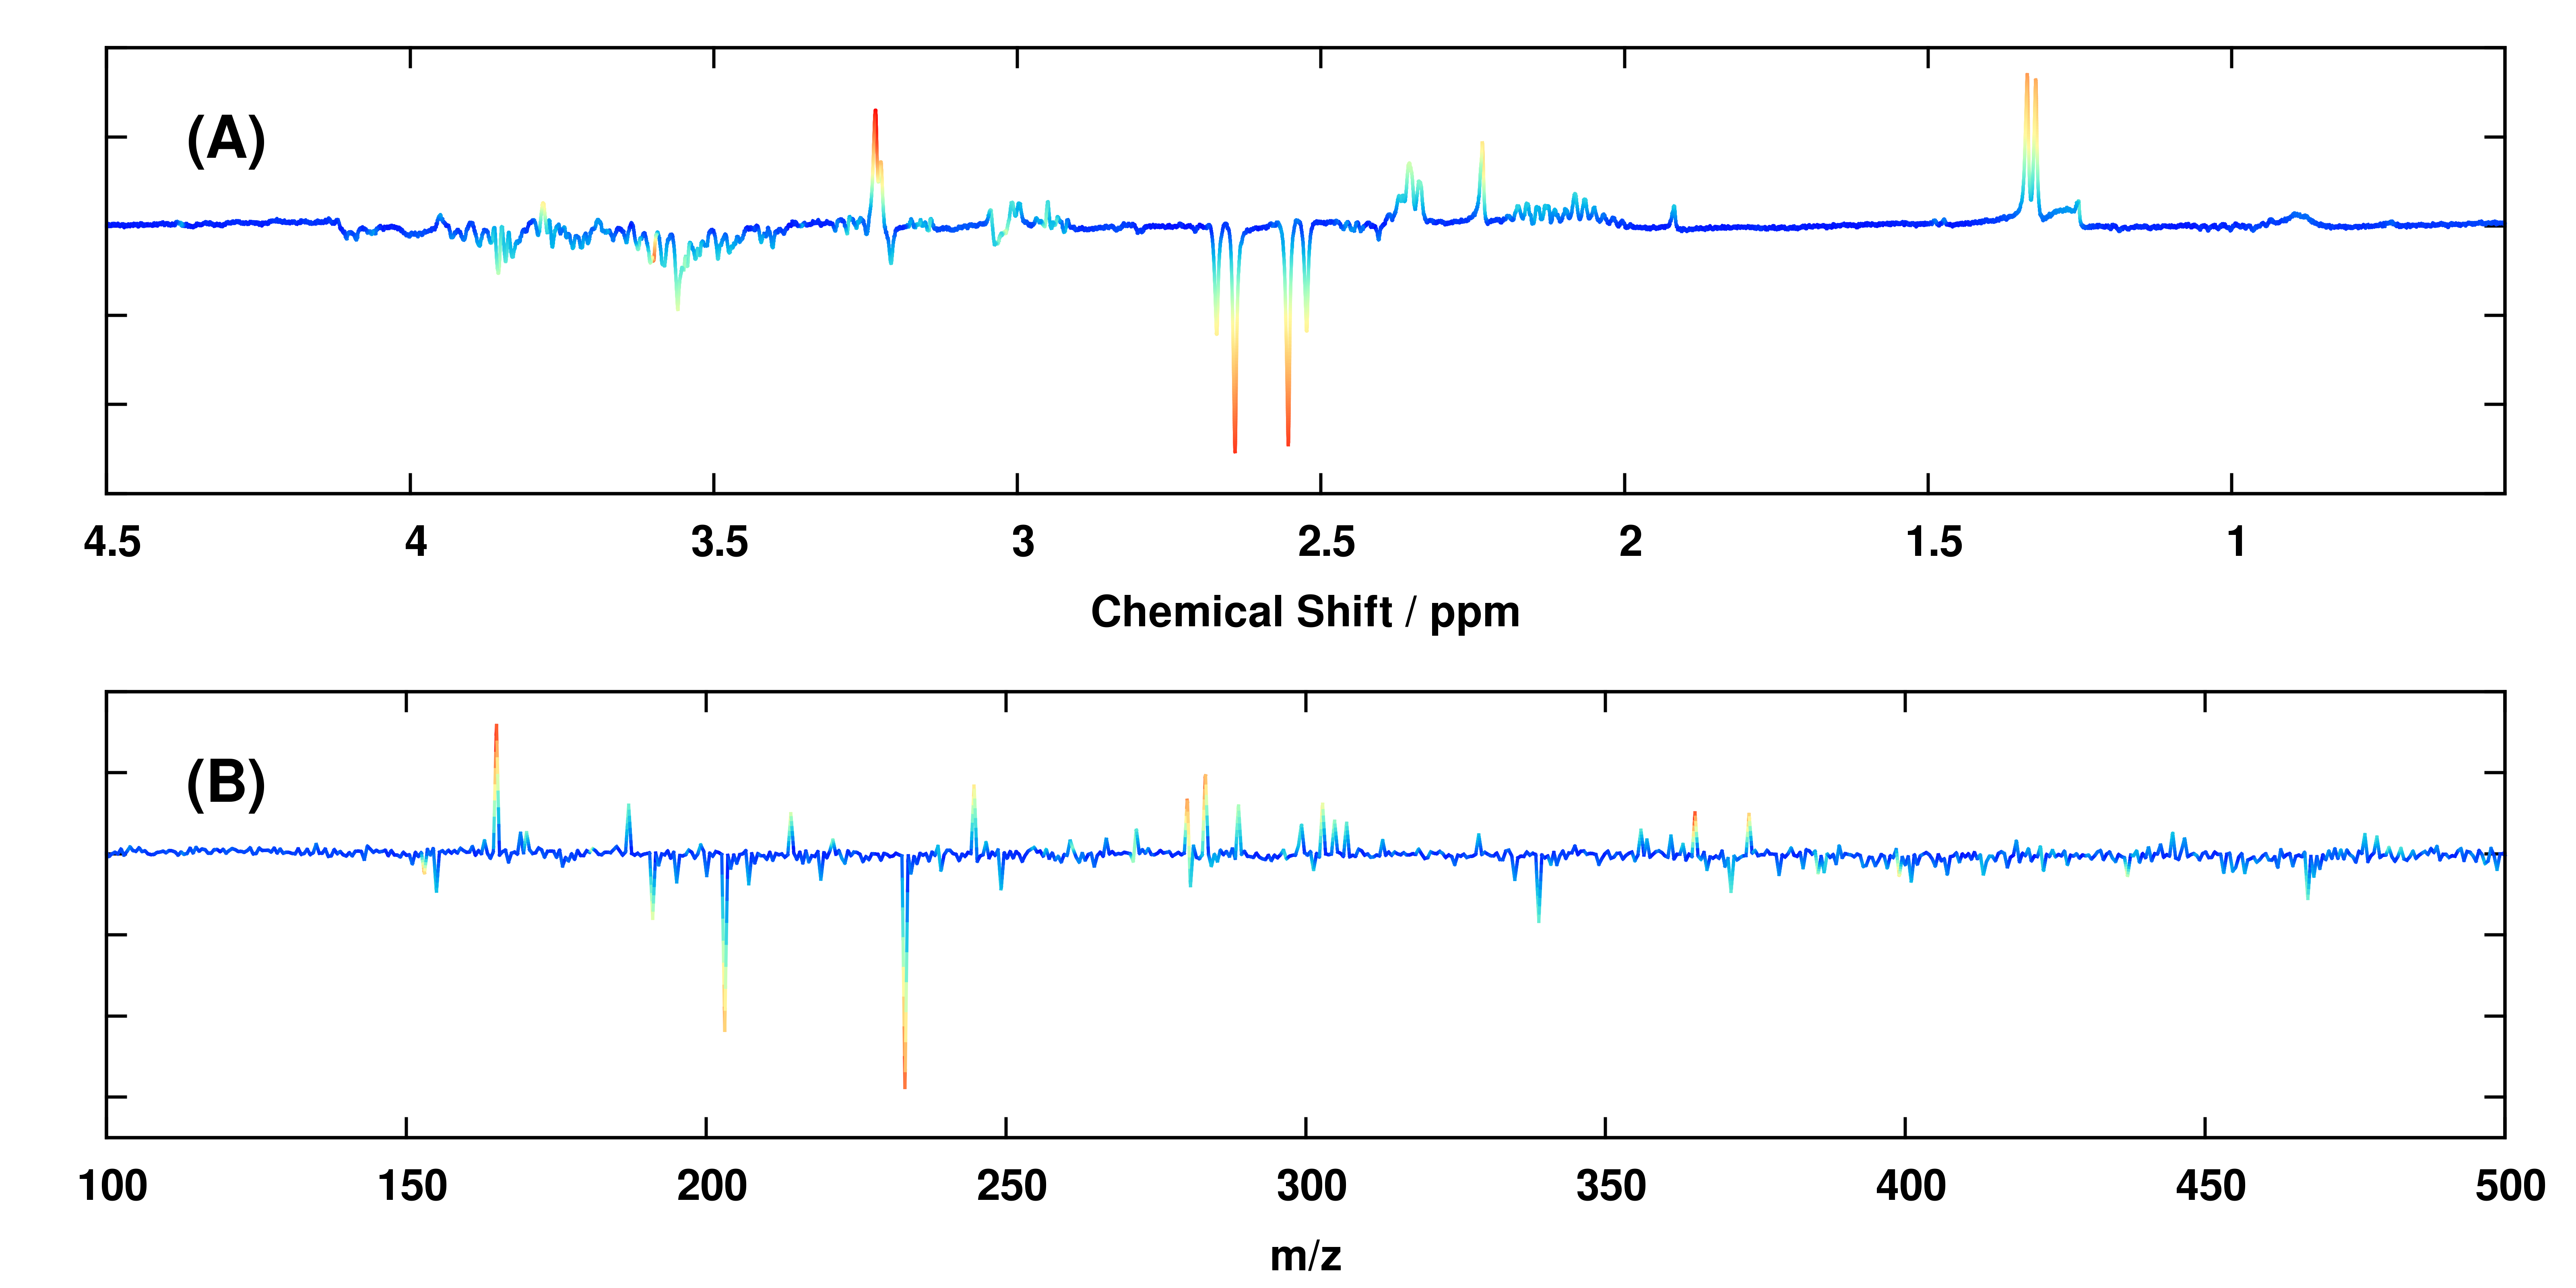
\includegraphics[width=6.5in]{figs/apps/13-mbopls-po.png}
\caption
      [Backscaled NMR and MS Orthogonal Block Loadings.]{
  {\bf Backscaled NMR and MS Orthogonal Block Loadings.}
  \\
  Backscaled orthogonal ({\bf A}) \hnmr{} NMR block and ({\bf B}) DI-ESI-MS
  block loadings from MB-OPLS-DA.
}
\end{figure}

\begin{doublespace}
MB-PLS of the data yielded similar improvements in model information content.
Two significant components were identified
($R^2_Y = 0.9876, Q^2 = 0.9014 \pm 0.0185$) that clearly separated control and
paraquat treatment classes from all other classes in scores space
(Figure 4.10). CV-ANOVA testing produced a $p$ value of $3.4 \times 10^{-4}$
and response permutation testing yielded $p < 0.001$, indicating a reliable
MB-PLS-DA model. Backscaled first-component MB-PLS-DA loadings are shown in
Figure 4.11. Modeling the multiblock data with MB-OPLS and MCCV produced a
single predictive component and a single orthogonal component
($R^2_Y = 0.9031, Q^2 = 0.7084 \pm 0.0241$), making later interpretation
markedly simpler (cf. Figures 4.12 and 4.13). Examination of cross-validated
MB-OPLS-DA scores (Figure 4.14) provides an excellent example of how PLS mixes
predictive and compensatory variation. In MB-OPLS super-scores, paraquat
treatment is distinctly separated from other neurotoxin treatment classes along
the orthogonal component ($\mathbf{t_o}$). In the MB-PLS model, this
distinction between paraquat and other drug treatments becomes mixed with the
variation that separates the control class from all drug treatments. In effect,
the two effects have been disentagled in the MB-OPLS model, providing richer
information about the differing mechanisms of each neurotoxic drug. Additional
orthogonal components would serve to further disentangle the two effects, at
the slight expense of model reliability. Validation of the MB-OPLS model by
CV-ANOVA resulted in a $p$ value equal to $5.5 \times 10^{-6}$, and permutation
testing corroborated CV-ANOVA with $p < 0.001$, once again indicating a
reliable supervised model.
\end{doublespace}

\begin{SCfigure}
\includegraphics[width=3.5in]{figs/apps/14-mbopls-t.png}
\caption
      [MB-OPLS-DA Cross-validated Scores.]{
  {\bf MB-OPLS-DA Cross-validated Scores.}
  \\
  Cross-validated scores generated from MB-OPLS-DA of the joint \hnmr{} NMR
  and DI-ESI-MS data. The OPLS filter within MB-OPLS has effectively rotated
  the super-scores of the MB-PLS model (Figure 4.10C) to better differentiate
  between class-predictive and class-orthogonal variation.
}
\end{SCfigure}

\subsection{Conclusions}

\begin{doublespace}
The use of multiblock bilinear factorizations that capitalize on the
availability of blocking information afforded greater model interpretability
with the NMR and MS data than what was provided by single-block methods. The
neurotoxins dataset provided an opportunity to compare the results of LOOCV
and MCCV for optimal principal component count determination when marginally
predictive data is being modeled. As expected, MCCV was a less optimistic
estimator of model reliability than LOOCV, and produced more parsimonious PCA
decompositions. Finally, the dataset was an ideal proving ground for the new
MB-OPLS algorithm, as MB-PLS-DA had clearly mixed class-predictive variation
into multiple components. The use of MB-OPLS-DA resulted in more easily
interpretable backscaled loadings, and provided more information relating to
separations between control and drug treatment \emph{and} separations between
paraquat and other drug treatments (Figure 4.13).
\end{doublespace}

\section{Monte Carlo Analysis of Scores-space Separations}

\begin{doublespace}
FIXME \cite{worley:anchem2015}.
\end{doublespace}

\subsection{Materials and Methods}

\begin{doublespace}
FIXME.
\end{doublespace}

\subsubsection{Initial Datasets}

\begin{doublespace}
Two classes of observations (Light and Medium Decaffeinated) from the binned
data matrix were extracted from the latest version of the Coffees
dataset \cite{worley:acscb2014}. The resulting data matrix (referred to as
$\mathbf{X}$: $N = 32, K = 284$) contains a highly significant separation
between the two classes based on caffeine 1D \hnmr{} NMR spectral features.
A second dataset, generated from a comparison of two chemically defined cell
growth media, was used to provide further support for the trends observed
during Monte Carlo analysis of the Coffees data matrix. The resulting Media
data matrix ($N = 50, K = 238$) also contains highly significant separation
between two classes based on 1D \hnmr{} NMR spectral features.
\\\\
Prior to Monte Carlo simulation, the $\ell_2$ norm (largest singular value) of
each data matrix $\mathbf{X}$ was computed and stored as $\sigma_{max}$. A set
of 50 noise standard deviations ($\sigma$) where each value ranged from
$\sigma_{max}/500$ to $\sigma_{max}/10$. For each noise standard deviation,
a set of 200 Monte Carlo iterations was performed. Another set of 200
iterations was also performed on each original data matrix $\mathbf{X}$ without
any added noise.
\end{doublespace}

\subsubsection{Monte Carlo Simulation}

\begin{doublespace}
At each Monte Carlo iteration, an $N \times K$ real matrix of noise values was
drawn as $NK$ independently and identically distributed samples from a
zero-mean normal distribution having a standard deviation of $\sigma$,
corresponding to the current noise value as described above. The data matrix
$\mathbf{X}$ was summed with the noise matrix, and a three-component ($A = 3$)
PCA model was computed on the resulting sum ($\mathbf{X'}$) after unit variance
scaling \cite{vandenberg:bmcg2006} using a NIPALS algorithm
\cite{jolliffe2002}. The explained variation (\rsq{}) of each principal
component was computed as described in \hyperlink{section.3.6}{Section 3.6}.
A Monte Carlo leave-$n$-out cross-validation (MCCV) was performed based on the
modified method of Krzanowski and Eastment \cite{eshghi:cils2014} in order to
obtain a per-component predictive ability (\qsq{}) statistic. A seven-fold
partitioning of observations and variables, randomly resampled ten times, was
performed for each PCA MCCV run. Following PCA model training, the Mahalanobis
distance between the two classes was computed using PCA scores
\cite{demaesschalck:cils2000}.
\\\\
After computation of the Mahalanobis distance, the noisy data matrix
$\mathbf{X'}$ was Pareto-scaled and subjected to OPLS-DA using a Pareto-scaled
binary $(0,1)$ response vector ($\mathbf{y}$) and a NIPALS OPLS algorithm
\cite{trygg:jchem2002}. A one-component ($A_p = 1, A_o = 1$) OPLS model was
constructed, from which backscaled predictive loadings were extracted by
dividing by the coefficients obtained from Pareto scaling
\cite{cloarec:anchem2005b}. The Pearson correlation coefficient between
backscaled loadings and the known `true' loadings --
$\mathrm{corr}(\mathbf{p},\mathbf{p_0})$ -- was computed for later
visualization. Explained variation (\rsqy{}) was computed as described in
\hyperlink{section.3.6}{Section 3.6}. A Monte Carlo leave-$n$-out internal
cross-validation of the OPLS model was performed using a seven-fold
partitioning of the data matrix that was randomly resampled ten times
\cite{xu:cils2001}. Predictive ability (\qsq{}) statistics were computed as
the mean \qsq{} obtained from MCCV results. Thus, each OPLS model contained
a set of ten fitted residual matrices from cross-validation available for use
in CV-ANOVA significance testing \cite{eriksson:jchemo2008}. During CV-ANOVA
calculations, the median values of mean square error (MSE) was computed from
all residual matrices, and the ratio of median fitted MSE to median residual
MSE was calculated to yield an $F$-statistic for $p$ value generation.
\end{doublespace}

\subsection{Results and Discussion}

\begin{doublespace}
FIXME.
\end{doublespace}

\section{Conclusions}

\begin{doublespace}
FIXME.
\end{doublespace}

\bibliographystyle{abbrv}
\bibliography{bworley}



\chapter{The MVAPACK Suite for NMR Chemometrics}

\section{Introduction}

\begin{doublespace}
The biochemical laboratory procedures involved in metabolomics experiments
are potentially straightforward and inexpensive, depending on the biological
systems and pathways under study \cite{zhang:jiomic2013}. The minimal sample
handling requirements of 1D \hnmr{} NMR spectroscopy and the immense
sensitivity of multivariate bilinear factorizations such as principal component
analysis (PCA) and partial least squares (PLS) make NMR metabolic
fingerprinting especially attainable. This low barrier to entry has no doubt
contributed to the rapid recent growth of the field. Unfortunately, the data
handling tasks of NMR metabolomics are far more difficult to properly execute.
Commercial software packages available for multivariate analysis (e.g. SIMCA,
PLS Toolbox, The Unscrambler, etc.) tend to be expensive and require more
software for upstream processing and treatment of spectral data. Analysts are
thus required to first open and process NMR data in packages such as ACD/1D NMR
Manager (Advanced Chemistry Development), Mnova NMR (Mestrelabs Research) and
perform further statistical treatment in MATLAB (The Mathworks, Natick, MA), R,
or Microsoft Excel. This results in an unnecessarily cumbersome and
time-consuming data handling pipeline by forcing the analyst to pass data
between multiple software packages. As a result, the field of metabolomics
research is littered with unpublished ``in-house'' software solutions created
for processing, treating or modeling NMR datasets
\cite{viant:bbrc2003,
      verhoeckx:immpc2004,
      cloarec:anchem2005a,
      cloarec:anchem2005b,
      dieterle:anchem2006,
      kang:food2008,
      wiklund:anchem2008}. This continued reinvention of the wheel impedes
progress in the field and complicates the tasks of standardization and
communication of protocols that the metabolomics community is desperately
attempting to achieve \cite{lindon:nbiot2005,goodacre:metab2007}. Insult is
then added to injury, as these in-house solutions are far less likely than
their commercial counterparts to include proper means of validating trained
multivariate models, further contributing to the general lack of model
validation already present in the field \cite{westerhuis:metab2008a}. While
the community has released several official software packages targeted at
metabolomics
\cite{jarvis:binf2006,
      daszykowski:cils2007,
      wang:bmcb2009,
      izquierdo:bmcb2009,
      xia:nar2012,
      gaude:cmb2013,
      alonso:anchem2014}, none provide a complete, well-validated data path.
At the time of this writing, no single software package existed to bring raw
NMR data along its complete journey to validated, interpretable multivariate
models.
\\\\
These issues motivated the development of a free and open-source software
package, MVAPACK, that provides a complete pipeline of functions for NMR
chemometrics and metabolomics. MVAPACK is written in the GNU Octave
mathematical programming language \cite{eaton2008}, which is also open-source
and nearly syntactically identical to MATLAB. Thus, the installation of
GNU/Linux, Octave and MVAPACK onto a commodity workstation provides a uniform
environment in which a data analyst may truly work ``from FIDs to models'' in
a few minutes using a set of well-documented, open-source, high-level data
handling functions.
\end{doublespace}

\begin{figure}[ht!]
\begin{center}
  \includegraphics[width=6in]{figs/mvapack/01-flow.png}
\end{center}
\caption
      [Example Data Handling Flow in MVAPACK.]{
  {\bf Example Data Handling Flow in MVAPACK.}
  \\
  A general NMR metabolic fingerprinting data handling flow diagram ({\bf A})
  and its associated minimum working example MVAPACK scripts ({\bf B}). This
  minimalist data handling script is a simple starting point for using
  MVAPACK; much greater flexibility and functionality are present in the
  software than may be shown here. All functions in bold typeface are provided
  in MVAPACK.
}
\label{figure.5.1}
\end{figure}

\section{Materials and Methods}

\subsection{Software Implementation}

\begin{doublespace}
The MVAPACK software package is written in GNU Octave, an open-source
mathematical programming language that uses MATLAB syntax \cite{eaton2008}.
Every function available in MVAPACK is realized as a single Octave function
file that may be examined or changed using any text editor. Most functions in
MVAPACK follow a similar input-to-output template, where an input data matrix
$\mathbf{A}$ is modified and returned as an output data matrix $\mathbf{B}$.
Other input arguments, required or optional, may accompany $\mathbf{A}$, and
extra output values may accompany $\mathbf{B}$, depending on the specific
needs of the analyst. Models produced by PCA, PLS, OPLS, LDA, MB-PCA and
MB-PLS are all similarly organized into Octave structures (i.e. ``structs'')
that all follow scalar, vector, and matrix notations of Wold et al.
\cite{wold:cils2001}. Thus, functions in MVAPACK are highly modular, often
allowing drop-in replacement of one processing, treatment or modeling method
for another by a simple change of function name and arguments. For instance,
all modeling algorithms allow the specification of a scaling method at the
time they are trained, so all available scaling functions conform to the
same interface: for any input data matrix, a scaled data matrix is returned
alongside the centering and scaling vectors used to compute the matrix.
\\\\
Data may be handled in MVAPACK in either interactive mode, in which the user
types commands into the Octave interpreter one at a time, or in batch mode,
where a complete processing scheme has been laid out in an Octave script to
be executed non-interactively. Once an ideal set of data handling steps is
determined by interactive manipulation of any given dataset, it may be
immortalized in an Octave script, thus providing documentation of procedures
and allowing for rapid recalculation of all associated results.
\\\\
\figref{5.1}{Figure 5.1} illustrates a simple MVAPACK script capable of taking
1D \hnmr{} NMR data from raw free induction decays to validated PCA and
OPLS-DA models. In section 1, a binary class matrix $\mathbf{Y}$ and an
accompanying set of class labels are built, and the time-domain raw data
are loaded into the complex data matrix $\mathbf{F}$. In section 2, the
time-domain data matrix $\mathbf{F}$ is zero-filled once and
Fourier-transformed to produce the complex spectral data
matrix $\mathbf{S}$. Section 3 automatically phase corrects each spectrum in
$\mathbf{S}$, normalizes and corrects for between-spectrum phase differences,
and corrects the chemical shift abscissa to center the reference peak at $0.0$
ppm. In sections 4 and 5, data handling splits into two pathways, where
icoshift alignment \cite{savorani:jmr2010} is used to generate a data matrix
$\mathbf{A}$ fit for full-resolution OPLS-DA and AI-binning
\cite{demeyer:anchem2008} is used to generate a data matrix $\mathbf{B}$ for
PCA. In section 6, a PCA model is built and assigned classes and labels, and
a model quality plot and a scores plot are produced. In section 7, similar
functions are used to train an OPLS-DA model and produce summary plots.
Finally, section 8 performs CV-ANOVA \cite{eriksson:jchemo2008} and response
permutation \cite{westerhuis:metab2008a} significance tests to fully validate
the supervised OPLS-DA model. While \figref{5.1}{Figure 5.1} is completely
functional, it is still an extremely bare-bones approach to metabolic
fingerprinting. MVAPACK provides countless other functions and schemes
for handling data.
\end{doublespace}

\subsection{Feature Set}

\begin{doublespace}
The functions available in MVAPACK span the following general categories:
data loading and processing (Table 5.1), treatment (Table 5.2),
modeling (Table 5.3), and validation (Table 5.4) \cite{goodacre:metab2007}.
Specific features in each category are discussed in the following sections.
\end{doublespace}

\begin{table}[h!]
\caption{MVAPACK Processing Feature Matrix.}
\begin{center}
\begin{tabular}{l l | l l l l l l l l l l l l l l l l}
  \hline
  & &
  \rot{Topspin} &
  \rot{VnmrJ} &
  \rot{nmrPipe} &
  \rot{NMRViewJ} &
  \rot{MNova} &
  \rot{ACD/NMR} &
  \rot{Automics} &
  \rot{Chenomx} &
  \rot{KnowItAll} &
  \rot{Metabonomic} &
  \rot{MetaboAnalyst} &
  \rot{AMIX} &
  \rot{SIMCA} &
  \rot{PLS Toolbox} &
  \rot{PyChem} &
  \rot{\bf MVAPACK} \\
  \hline
  \multicolumn{2}{l|}{{\bf Loading}} & & & & & & & & & & & & & & & & \\
  & Bruker, 1D
  & * &   & * & * & * & * & * & * & * & * &   & * &   &   &   & * \\
  & Bruker, 2D
  & * &   & * & * & * & * &   &   &   &   &   &   &   &   &   & * \\
  & Varian, 1D
  &   & * & * & * & * & * & * & * & * &   &   & * &   &   &   & * \\
  \multicolumn{2}{l|}{{\bf Apodization}} & & & & & & & & & & & & & & & & \\
  & Exponential, 1D
  & * & * & * &   & * & * &   & * & * &   &   &   &   &   &   & * \\
  & Exponential, 2D
  & * & * & * &   & * & * &   &   &   &   &   &   &   &   &   & * \\
  & Gaussian, 1D
  & * & * & * &   & * & * &   &   & * &   &   &   &   &   &   & * \\
  & Gaussian, 2D
  & * & * & * &   & * & * &   &   &   &   &   &   &   &   &   & * \\
  & Sine, 1D
  & * & * & * &   & * & * &   &   &   &   &   &   &   &   &   & * \\
  & Sine, 2D
  & * & * & * &   & * & * &   &   &   &   &   &   &   &   &   & * \\
  \multicolumn{2}{l|}{{\bf Zero-filling}} & & & & & & & & & & & & & & & & \\
  & ZF, 1D
  & * & * & * &   & * & * & * & * & * &   &   &   &   &   &   & * \\
  & ZF, 2D
  & * & * & * &   & * & * &   &   &   &   &   &   &   &   &   & * \\
  \multicolumn{2}{l|}{{\bf Transforms}} & & & & & & & & & & & & & & & & \\
  & DFT, 1D
  & * & * & * &   & * & * & * & * & * & * &   &   &   &   &   & * \\
  & DFT, 2D
  & * & * & * &   & * & * &   &   &   &   &   &   &   &   &   & * \\
  & CWT, 1D
  &   &   &   &   & * &   &   &   &   &   &   &   & * &   &   & * \\
  & IST, 2D
  & * & * &   &   & * &   &   &   &   &   &   &   &   &   &   & * \\
  \multicolumn{2}{l|}{{\bf Phase correction}} & & & & & & & & & & & & & & & & \\
  & Manual, 1D
  & * & * & * &   & * & * & * & * & * & * &   & * &   &   &   & * \\
  & Manual, 2D
  & * & * & * &   & * & * &   &   &   &   &   & * &   &   &   & * \\
  & Automatic, 1D
  & * & * &   &   & * & * & * & * & * &   &   & * &   &   &   & * \\
  & Automatic, 2D
  & * & * &   &   & * & * &   &   &   &   &   &   &   &   &   & *
\end{tabular}
\end{center}
\end{table}

\subsubsection{Processing}

\begin{doublespace}
Loading of Bruker raw data is available using either a high-performance
DMX-format loading routine or nmrPipe \cite{delaglio:jbnmr1995} as a backend,
and loading of Varian data is available using an nmrPipe backend. Additionally,
data in a variety of structured text formats may be read into MVAPACK using
standard GNU Octave routines. The NMR spectral processing functions in MVAPACK
follow the traditional paradigms of NMR processing \cite{hoch1996} and include
methods for apodization, zero-filling, Fourier transformation, Iterative Soft
Thresholding (IST) reconstruction \cite{hyberts:jacs2007}, manual and automatic
phase correction
\cite{siegel:aca1981,chen:jmr2002,balacco:mrc2009}, region of interest
selection and manipulation, peak picking \cite{du:binf2006}, integration and
referencing.
\end{doublespace}

\begin{table}[h!]
\caption{MVAPACK Treatment Feature Matrix.}
\begin{center}
\begin{tabular}{l l | l l l l l l l l l l l l l l l l}
  \hline
  & &
  \rot{Topspin} &
  \rot{VnmrJ} &
  \rot{nmrPipe} &
  \rot{NMRViewJ} &
  \rot{MNova} &
  \rot{ACD/NMR} &
  \rot{Automics} &
  \rot{Chenomx} &
  \rot{KnowItAll} &
  \rot{Metabonomic} &
  \rot{MetaboAnalyst} &
  \rot{AMIX} &
  \rot{SIMCA} &
  \rot{PLS Toolbox} &
  \rot{PyChem} &
  \rot{\bf MVAPACK} \\
  \hline
  \multicolumn{2}{l|}{{\bf Binning}} & & & & & & & & & & & & & & & & \\
  & Uniform, 1D
  &   &   &   &   & * & * & * &   & * & * &   & * &   &   &   & * \\
  & Uniform, 2D
  &   &   &   &   &   & * & * &   & * &   &   & * &   &   &   & * \\
  & Optimized, 1D
  &   &   &   &   &   &   &   &   &   &   &   & * &   &   &   & * \\
  & Adaptive, 1D
  &   &   &   &   &   &   &   &   &   &   &   & * &   &   &   & * \\
  & Adaptive, 2D
  &   &   &   &   &   &   &   &   &   &   &   &   &   &   &   & * \\
  \multicolumn{2}{l|}{{\bf Alignment}} & & & & & & & & & & & & & & & & \\
  & Global
  &   &   &   &   &   &   & * &   &   &   &   &   &   &   &   & * \\
  & Interval
  &   &   &   &   &   &   & * &   &   &   &   &   &   &   &   & * \\
  \multicolumn{2}{l|}{{\bf Normalization}} & & & & & & & & & & & & & & & & \\
  & CS
  &   &   &   &   &   &   &   &   &   &   & * & * &   & * & * & * \\
  & PQ
  &   &   &   &   &   &   &   &   &   &   & * &   &   &   &   & * \\
  & HM
  &   &   &   &   &   &   &   &   &   &   &   &   &   &   &   & * \\
  & SNV
  &   &   &   &   &   &   & * &   & * & * &   & * &   & * & * & * \\
  & MSC
  &   &   &   &   &   &   & * &   & * &   &   &   &   & * & * & * \\
  & PSC
  &   &   &   &   &   &   &   &   &   &   &   &   &   &   &   & * \\
  \multicolumn{2}{l|}{{\bf Scaling}} & & & & & & & & & & & & & & & & \\
  & UV
  &   &   & * &   &   &   & * &   & * & * & * & * & * & * & * & * \\
  & Pareto
  &   &   &   &   & * &   & * &   & * & * & * &   & * &   &   & * \\
  & Range
  &   &   &   &   & * &   &   &   & * & * & * &   & * &   &   & * \\
  & Level
  &   &   &   &   & * &   &   &   &   &   &   &   & * &   &   & * \\
  & VAST
  &   &   &   &   & * &   &   &   & * &   &   &   & * &   &   & *
\end{tabular}
\end{center}
\end{table}

\subsubsection{Treatment}

\begin{doublespace}
Functions for statistical data treatment in MVAPACK include binning
\cite{sousa:cils2013,demeyer:anchem2008}, alignment \cite{savorani:jmr2010},
normalization \cite{barnes:aspec1989,dieterle:anchem2006,torgrip:metab2008},
scaling \cite{vandenberg:bmcg2006}, and direct orthogonal signal correction
\cite{westerhuis:cils2001}. In addition, MVAPACK supports uniform binning
and AI-binning (\hyperlink{chapter.6}{Chapter 6}) of third-order data tensors
stored as arrays of real matrices in Octave.
\end{doublespace}

\begin{table}[h!]
\caption{MVAPACK Modeling Feature Matrix.}
\begin{center}
\begin{tabular}{l l | l l l l l l l l l l l l l l l l}
  \hline
  & &
  \rot{Topspin} &
  \rot{VnmrJ} &
  \rot{nmrPipe} &
  \rot{NMRViewJ} &
  \rot{MNova} &
  \rot{ACD/NMR} &
  \rot{Automics} &
  \rot{Chenomx} &
  \rot{KnowItAll} &
  \rot{Metabonomic} &
  \rot{MetaboAnalyst} &
  \rot{AMIX} &
  \rot{SIMCA} &
  \rot{PLS Toolbox} &
  \rot{PyChem} &
  \rot{\bf MVAPACK} \\
  \hline
  \multicolumn{2}{l|}{{\bf Bilinear}} & & & & & & & & & & & & & & & & \\
  & PCA
  &   &   & * &   & * &   & * &   & * & * & * & * & * & * & * & * \\
  & LDA
  &   &   &   &   &   &   & * &   &   &   &   & * &   &   &   & * \\
  & PLS
  &   &   &   &   &   &   & * &   &   & * & * & * & * & * &   & * \\
  & OPLS
  &   &   &   &   &   &   &   &   &   &   &   &   & * & * &   & * \\
  \multicolumn{2}{l|}{{\bf Multiblock}} & & & & & & & & & & & & & & & & \\
  & MB-PCA
  &   &   &   &   &   &   &   &   &   &   &   &   &   & * &   & * \\
  & MB-PLS
  &   &   &   &   &   &   &   &   &   &   &   &   &   & * &   & * \\
  & MB-OPLS
  &   &   &   &   &   &   &   &   &   &   &   &   &   &   &   & *
\end{tabular}
\end{center}
\end{table}

\subsubsection{Modeling}

\begin{doublespace}
MVAPACK provides complete support for building PCA \cite{jolliffe2002},
LDA \cite{hardle2012}, PLS \cite{wold1993,geladi:aca1986,wold:cils2001},
OPLS \cite{trygg:jchemo2002,bylesjo:jchemo2006}, MB-PCA and MB-PLS
\cite{westerhuis:jchemo1998,smilde:jchemo2003} models from processed
and treated datasets. At the current time, only bilinear factorizations
are supported within MVAPACK.
\end{doublespace}

\begin{table}[h!]
\caption{MVAPACK Validation Feature Matrix.}
\begin{center}
\begin{tabular}{l l | l l l l l l l l l l l l l l l l}
  \hline
  & &
  \rot{Topspin} &
  \rot{VnmrJ} &
  \rot{nmrPipe} &
  \rot{NMRViewJ} &
  \rot{MNova} &
  \rot{ACD/NMR} &
  \rot{Automics} &
  \rot{Chenomx} &
  \rot{KnowItAll} &
  \rot{Metabonomic} &
  \rot{MetaboAnalyst} &
  \rot{AMIX} &
  \rot{SIMCA} &
  \rot{PLS Toolbox} &
  \rot{PyChem} &
  \rot{\bf MVAPACK} \\
  \hline
  \multicolumn{2}{l|}{{\bf Validation}} & & & & & & & & & & & & & & & & \\
  & \rsq{}, \qsq{}
  &   &   &   &   &   &   & * &   & * & * & * & * & * & * & * & * \\
  & Permutation
  &   &   &   &   &   &   &   &   &   &   & * &   & * & * &   & * \\
  & CV-ANOVA
  &   &   &   &   &   &   &   &   &   &   &   &   & * &   &   & * \\
  \multicolumn{2}{l|}{{\bf Visualization}} & & & & & & & & & & & & & & & & \\
  & 2D Scores
  &   &   &   &   & * &   & * &   & * & * & * & * & * & * & * & * \\
  & 3D Scores
  &   &   &   &   &   &   &   &   & * & * & * &   & * & * &   & * \\
  & Loadings
  &   &   &   &   & * &   & * &   & * & * & * & * & * & * & * & * \\
  & Backscaling
  &   &   &   &   &   &   &   &   &   &   &   &   &   &   &   & * \\
  & S-plot
  &   &   &   &   &   &   &   &   &   &   &   &   & * &   &   & * \\
  & SUS-plot
  &   &   &   &   &   &   &   &   &   &   &   &   & * &   &   & * \\
  & Data Ellipsoid
  &   &   &   &   &   &   &   &   &   & * & * & * & * & * &   & * \\
  & Class Ellipsoid
  &   &   &   &   &   &   &   &   &   &   &   &   &   &   &   & *
\end{tabular}
\end{center}
\end{table}

\subsubsection{Validation}

\begin{doublespace}
All PCA and MB-PCA models are validated as they are built based on the results
of a Monte Carlo leave-$n$-out (Modified $K+E$) internal cross-validation
\cite{eastment:tech1982,eshghi:cils2014}, and all PLS, OPLS and MB-PLS models
are validated during training based on results of a Monte Carlo leave-$n$-out
internal cross-validation \cite{xu:cils2001,xu:jchemo2004}. In all cases, a
set of \rsq{} (i.e. \rsqx{} and \rsqy{}) statistics are generated to assess
how well each data and response matrix is approximated by the models, and
\qsq{} statistics are generated to describe self-consistency and predictive
ability of each data matrix in PCA and PLS models, respectively. Per-component
\rsq{} and \qsq{} statistics are utilized by MVAPACK to estimate the optimal
number of model components. Because cross-validation is performed using a
Monte Carlo scheme in MVAPACK, all \qsq{} statistics are reported with
confidence intervals, regardless of model type. Further validation of
supervised models is available in the form of CV-ANOVA
\cite{eriksson:jchemo2008} and response permutation
\cite{westerhuis:metab2008a} significance testing, both of which report
$p$ values that indicate model validity.
\end{doublespace}

\section{Discussion and Conclusions}

\begin{doublespace}
This chapter presents MVAPACK, a completely free and open-source data handling
environment tailor-suited to NMR chemometrics and \hnmr{} NMR and MS metabolic
fingerprinting applications. Unlike data handling chains composed of multiple
commercial software packages, MVAPACK is free to use, modify and distribute
according to the GNU General Public License \cite{gpl3} and provides a single
consistent data handling environment. Because MVAPACK is written for GNU
Octave, researchers already familiar with MATLAB syntax will also be familiar
with MVAPACK without a considerable learning curve. Datasets and results
obtained using MVAPACK are readily saved and exchanged using GNU Octave
built-in support for the MATLAB \emph{mat}-file format.
\\\\
A recent review \cite{izquierdo:pnmrs2011} of software packages targeted at
metabolomics highlights the piecemeal nature of 1D \hnmr{} NMR data handling
in the field, where no single package is capable of performing all the tasks
required by the analyst. MVAPACK addresses this need by providing a complete
pipeline that is tuned for metabolic fingerprinting. Use of MVAPACK reduces
data analysis time in metabolic fingerprinting from days to minutes, simply
by collecting all the required functions into a single scriptable environment.
In fact, the example script in \figref{5.1}{Figure 5.1} would execute in under
five minutes on a modern GNU/Linux or Mac OS X computer system.
\\\\
The routine processing of {\it any} 1D and 2D NMR spectral data may be readily
done with MVAPACK, and processing routines are easily batched. The MVAPACK
scripts written to analyze the datasets in \hyperlink{chapter.4}{Chapter 4}
are composed of intuitive, modular commands that logically subdivide the script
into recognizable tasks like automatic phase correction, spectral alignment,
normalization, and so forth. Furthermore, aside from physical memory
limitations of the host computer, MVAPACK does not impose any limit
on the number of NMR observations that may be simultaneously handled.
\\\\
A major advantage of MVAPACK is the seamless transfer of the processed, treated
NMR data to multivariate statistical analyses. The PCA, PLS, OPLS and LDA
bilinear modeling algorithms, now ubiquitous in the metabolomics community,
are all implemented in MVAPACK using a consistent under-the-hood framework.
Model results may be visualized and interpreted using MVAPACK routines that
provide scatter, line and bar plots of model scores, loadings and validation
statistics. Critically, MVAPACK automatically ensures that {\it all} trained
models are valid using leave-one-out and Monte Carlo leave-$n$-out internal
cross-validation routines and provides further means of validating supervised
models in the form of CV-ANOVA and response permutation significance testing.
Several powerful examples of MVAPACK applied to real datasets are presented in
\hyperlink{chapter.4}{Chapter 4}. Because it implements well-established
algorithms available from peer-reviewed chemometrics literature, MVAPACK
generates identical results when compared to expensive software packages
like Umetrics SIMCA-P+.
\\\\
In short, MVAPACK provides a complete platform for NMR chemometric data
handling that is ideal for both routine handling of metabolomics datasets and
development of novel algorithms. Unlike its closed-source predecessors, the
modular, open-source design of MVAPACK readily accepts new functionality,
allowing it to grow and maintain pace with the state-of-the-art in the
chemometrics literature. MVAPACK is freely available for download at
\url{http://bionmr.unl.edu/mvapack.php}. Detailed documentation of MVAPACK,
all datasets presented in \hyperlink{chapter.4}{Chapter 4}, and the scripts
used to handle them are also available for download.
\end{doublespace}

\bibliographystyle{abbrv}
\bibliography{bworley}



\chapter{Phase-Scatter Correction of NMR Datasets}

\section{Introduction}

\begin{doublespace}
As previously introduced in \hyperlink{chapter.3}{Chapter 3}, normalization
of data tensors is a commonly performed procedure aimed at minimizing the
within-class variation of two or more groups of observations, relative to
the total or between-class variation in the dataset. Irrespective of whether
separations between classes are obtained using an unsupervised PCA model or a
supervised (O)PLS-DA model, greater statistical significance and increased
biological relevance may be ascribed to separations between classes having
greater variation between groups than within them \cite{worley:abio2013}.
\\\\
Normalization applied directly to hypercomplex NMR data (or its real component)
is sub-optimal, as even small phase differences between observations can
frustrate the estimation of normalization factors
(See \hyperlink{section.3.3}{Section 3.3}). Possibly worse, blind
normalization of poorly phased spectral data can accentuate experimentally
irrelevant spectral features in a data tensor during multivariate modeling,
leading the analyst to erroneous conclusions. These difficulties motivated
the development of phase-scatter correction (PSC, \cite{worley:cils2014}) as
a means of simultaneously correcting the coupled phase errors and dilution
errors that are present in hypercomplex NMR data tensors. When hypercomplex
NMR data must be normalized prior to multivariate analyses within the confines
of a metabolomics study, the interrelation of phase and dilution errors is best
handled using phase-scatter correction.
\end{doublespace}

\section{Theory}

\subsection{Multiplicative Scatter Correction}

\begin{doublespace}
Phase-scatter correction (PSC) is effectively an extension of multiplicative
scatter correction (MSC) to handle phase errors during normalization. In MSC,
each real spectrum is scaled around its mean intensity and shifted to match a
reference spectrum, typically the mean of the dataset \cite{fearn:cils2009}.
Optimal normalization factors ($\mathbf{b}$) of a data matrix $\mathbf{X}$ are
determined by a linear regression of the mean-centered reference vector onto
the mean-centered matrix:
\begin{equation}
\big( \mathbf{X} - \langle \mathbf{X} \rangle \big)^T \mathbf{b}
 = \big( \mathbf{r} - \langle \mathbf{r} \rangle \big)^T
\end{equation}
where observations are stored as row vectors in $\mathbf{X}$, and $\mathbf{r}$
is the reference observation row vector. The equation above represents an
overdetermined system of linear equations, therefore the least-squares estimate
of $\mathbf{b}$ may be computed rapidly, and MSC is rather computationally
efficient.
\end{doublespace}

\subsection{Phase-scatter Correction}

\begin{doublespace}
PSC additionally corrects zero- and first-order phase errors during
normalization, requiring a nonlinear optimization of the following objective:
\begin{equation}
Q(\mathbf{X} \mid \mathbf{p})
 = \sum_{n=1}^N \| \mathbf{z}_n \circ \mathbf{x}_n - \mathbf{r} \|_2^2
\end{equation}
where $\circ$ denotes the element-wise product, the mean-centered matrix
$\mathbf{X}$ lies in $\mathbb{H}_1^{N \times K}$, the mean-centered reference
$\mathbf{r}$ lies in $\mathbb{H}_1^K$, and the set of parameters $\mathbf{p}$
includes a normalization factor and two phase errors per observation
in $\mathbf{X}$:
\begin{equation}
\mathbf{p} = \{
  b_1, \dots b_N,
  \theta_{0,1}, \dots \theta_{0,N},
  \theta_{1,1}, \dots \theta_{1,N} \}
\end{equation}
and each vector $\mathbf{z}_n$ contains the normalization and phase corrections
for the $n$-th observation $\mathbf{x}_n$:
\begin{equation}
z_{n,k} = b_n e^{u_1 (\theta_{0,n} + \theta_{1,n} k)}
\end{equation}

Because the reference observation $\mathbf{r}$ is fixed during optimization,
minimization of $Q(\mathbf{X} \mid \mathbf{p})$ may be achieved by
independently minimizing each observation's contributions. Minimization is
carried out for every observation in the data matrix using Levenberg-Marquardt
nonlinear least squares \cite{marquardt:jsiam1963} as implemented by the
{\it leasqr} function in GNU Octave, a function similar to MATLAB's
{\it nlinfit}. Each corrected spectrum $\hat{\mathbf{x}}_n$ is then returned
from optimization as follows:
\begin{equation}
\hat{\mathbf{x}}_n
 = \mathbf{z}_n \circ \mathbf{x}_n
 + \langle \mathbf{r} \rangle
\end{equation}

Phase-scatter correction of 50 1D \hnmr{} NMR spectra having 32$k$ complex
points each requires approximately 30 seconds on a single-core 3.2 GHz Intel
workstation running GNU Octave 3.6.
\end{doublespace}

\subsection{Ensemble Phase Correction}

\begin{doublespace}
It is important recognize that the phase-scatter correction objective function
$Q(\mathbf{X} \mid \mathbf{p})$ provides no measure of ideal phase values,
meaning that PSC requires an additional phase correction step prior to its
execution in order to ensure adequate initial conditions. Even when
$\mathbf{X}$ has been suitably phase-corrected, PSC may still attempt to
minimize scatter between spectra by re-introducing phase errors. This
undesirable behavior of PSC may be observed when large disparities in
spectral intensities are present between observations. To correct this,
a standard phase correction objective
$f : \mathbb{H}_D^{K} \to \mathbb{R}$ may be combined with
the PSC objective using a Lagrange multiplier, like so:
\begin{equation}
\Lambda(\mathbf{X} \mid \mathbf{p}) =
 -\sum_{n=1}^N f(\boldsymbol{\theta}_n \circ \mathbf{x}_n) +
 \lambda \sum_{n=1}^N \| \mathbf{z}_n \circ \mathbf{x}_n -
            \langle \mathbf{Z} \circ \mathbf{X} \rangle \|_2^2
\end{equation}
where the correction matrix $\mathbf{Z}$ has the same form as in PSC, expressed
as a real diagonal matrix of normalization factors $\mathbf{B}$ and a
hypercomplex matrix of phase factors $\mathbf{\Theta}$:
\begin{equation}
\mathbf{Z} = \mathbf{B} \mathbf{\Theta}
\end{equation}
and $\boldsymbol{\theta}_n$ is the $n$-th row of $\mathbf{\Theta}$. The new
ensemble phase correction (EPC) objective function
$\Lambda(\mathbf{X} \mid \mathbf{p})$ balances the potentially opposing goals
of phase correction and scatter correction through the Lagrange multiplier
$\lambda$, and does not require the specification of a reference observation
$\mathbf{r}$. In effect, EPC allows its scatter correction reference to float
as the current mean of the data, $\langle \mathbf{Z} \circ \mathbf{X} \rangle$.
This floating reference requires the simultaneous optimization of all the
parameters in $\mathbf{p}$, unlike phase-scatter correction. Efficient
minimization of $\Lambda(\mathbf{X} \mid \mathbf{p})$ may be accomplished by
a modified Nelder-Mead simplex optimization procedure \cite{nelder:compj1964},
which serially updates the simplices of all observations at each global
iteration and maintains the current mean vector
$\langle \mathbf{Z} \circ \mathbf{X} \rangle$ at each update.
\\\\
In contrast to phase-scatter correction, which seeks to minimize the scatter
of data matrix observations around a fixed reference, ensemble phase correction
approaches the dilemma of entwined phase and normalization errors from an
opposing direction by introducing a scatter term into a standard automatic
phase correction procedure. The amount of normalization achieved by EPC is
directly controlled by the magnitude of $\lambda$: in the opposite limits of
$\lambda = 0$ and $\lambda \to \infty$, EPC becomes equivalent to standard
phase correction and phase-scatter correction with a floating reference,
respectively.
\end{doublespace}

\section{Materials and Methods}

\begin{SCfigure}
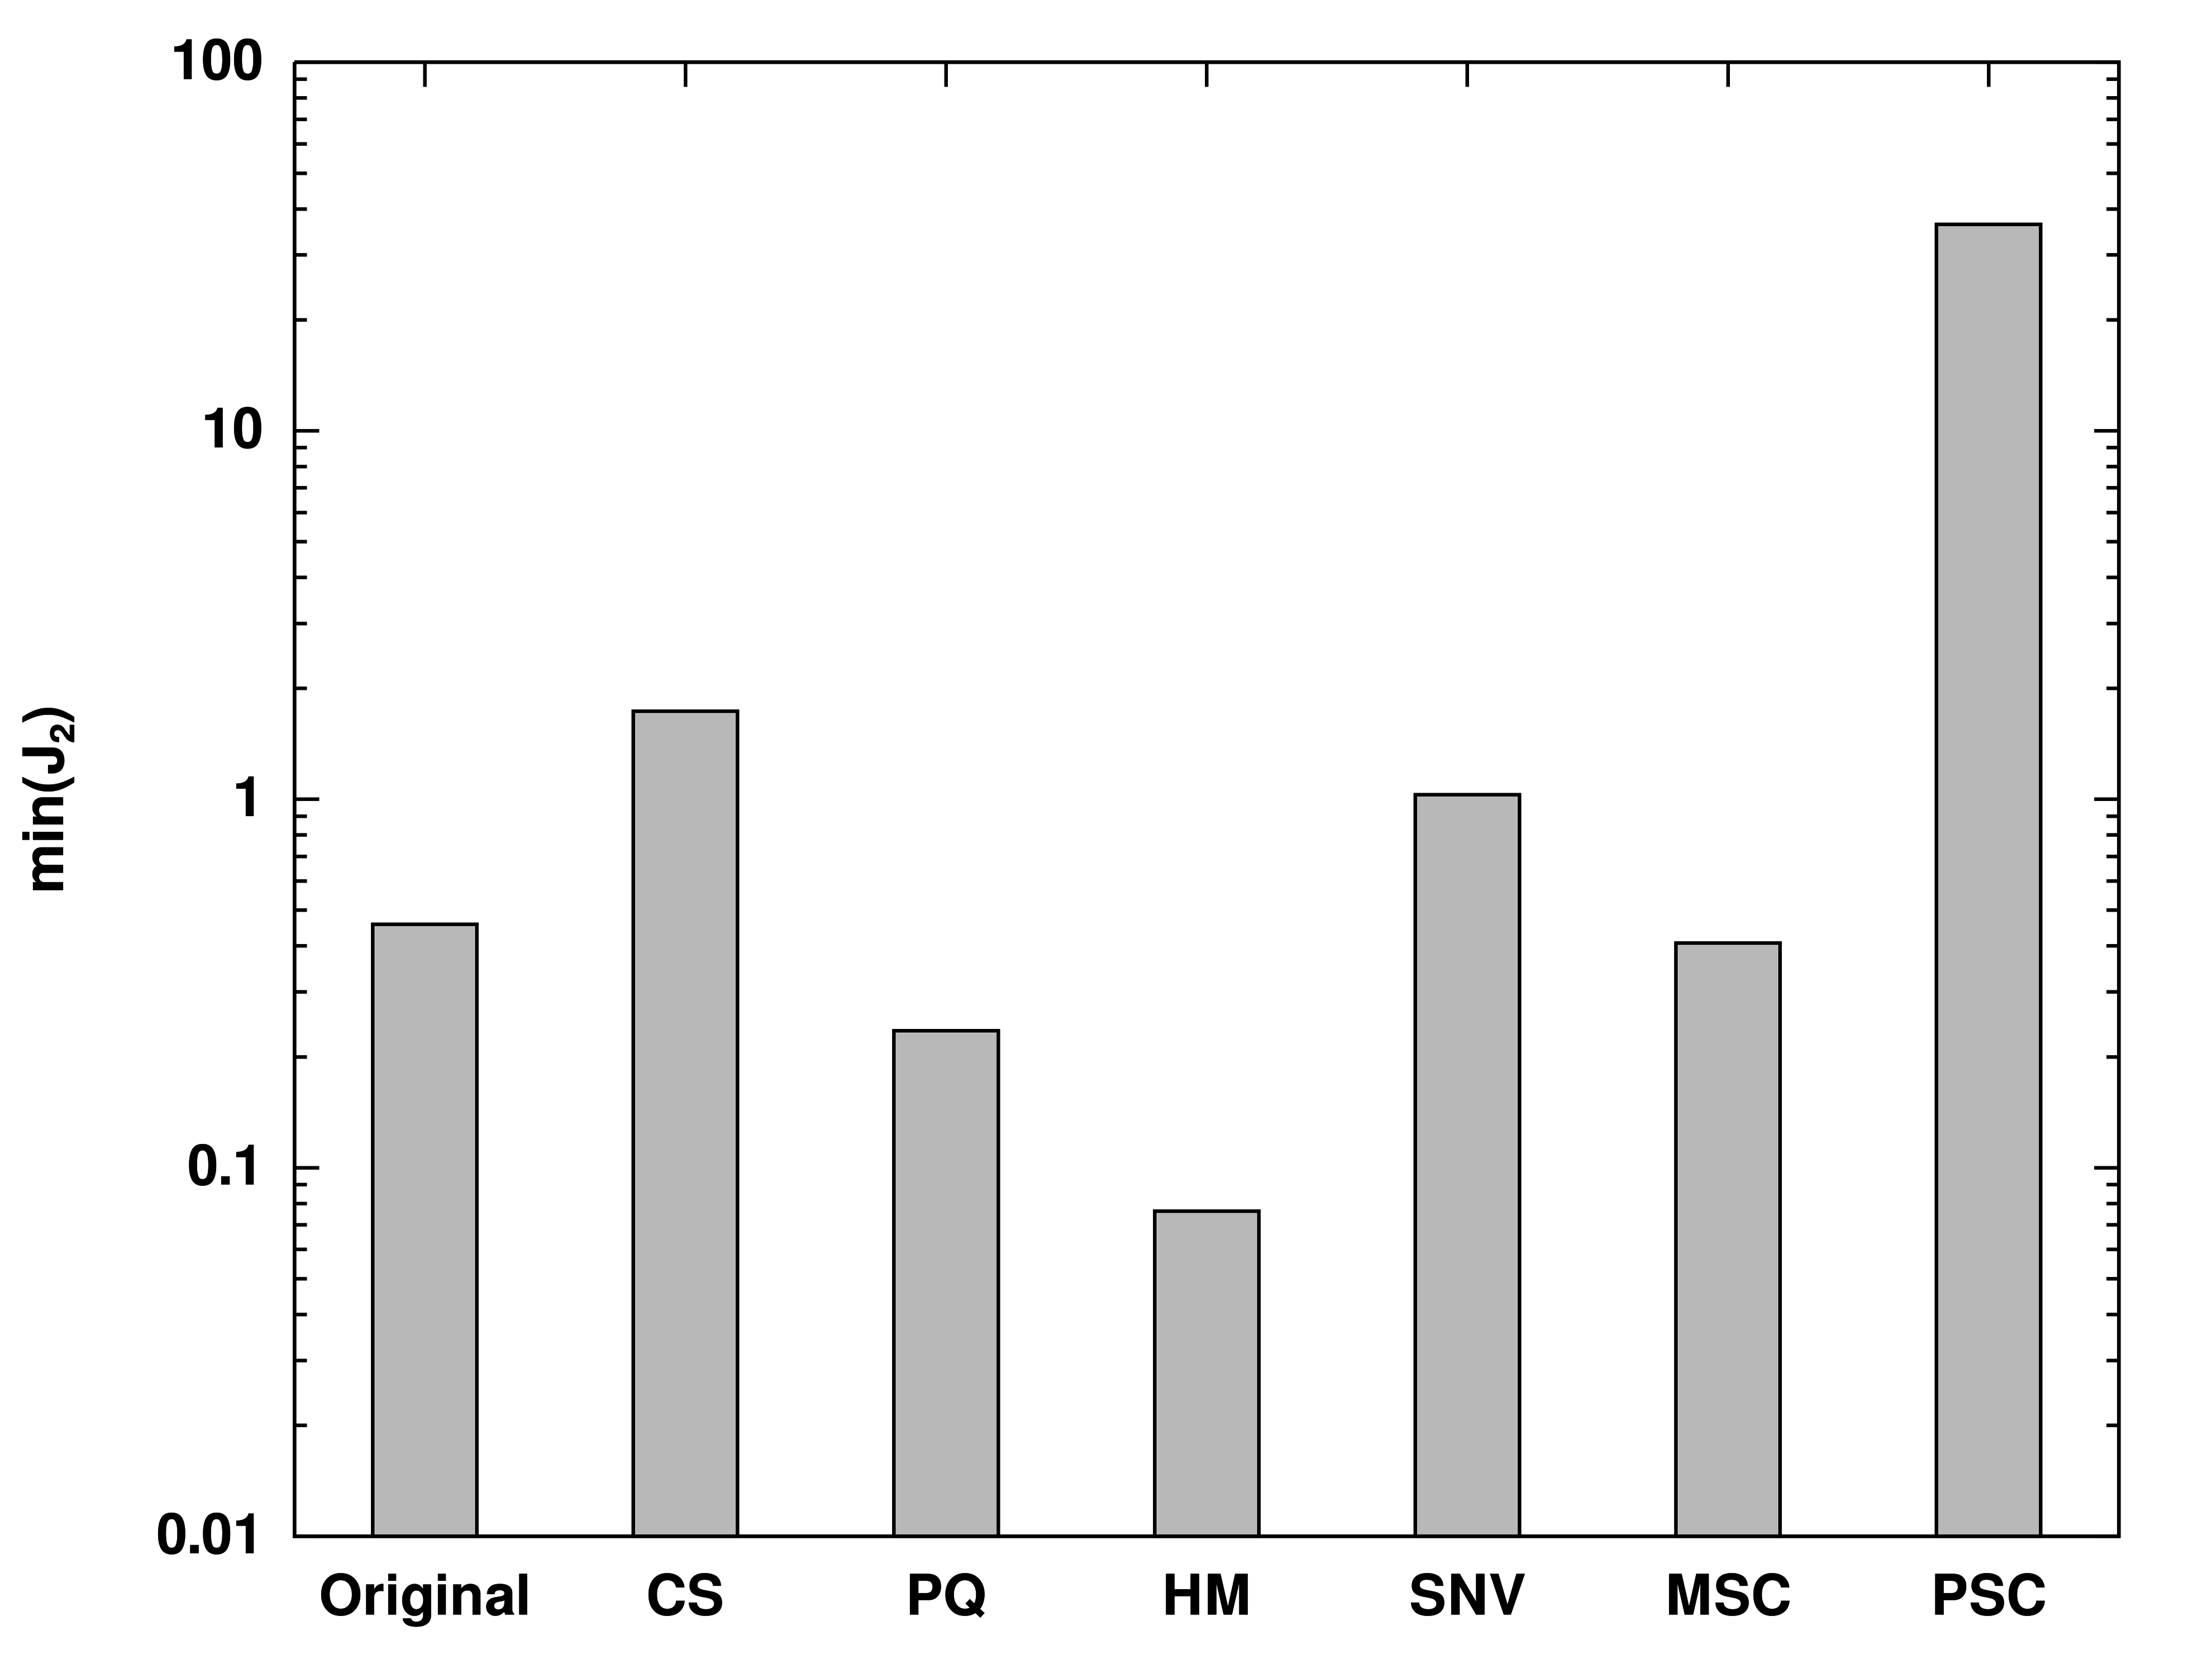
\includegraphics[width=3.5in]{figs/pscorr/01-minj2.png}
\caption
      [Cluster Quality after Normalization and PCA Modeling.]{
  {\bf Cluster Quality after Normalization and PCA Modeling.}
  \\
  Comparison of PCA cluster quality for \hnmr{} NMR metabolomics data
  normalized using different algorithms. The minimum $J_2$ value (worst
  cluster quality) for each model is reported here, as it is a more effective
  indicator of overall model and cluster quality than the mean or median.
}
\end{SCfigure}

\subsection{NMR Data Processing}

\begin{doublespace}
Previously collected \hnmr{} NMR spectral data from published work
\cite{halouska:acscb2012} was leveraged as a typical metabolomics dataset
for performance analysis of PSC versus other normalization methods. Free
induction decays were loaded into GNU Octave 3.6 \cite{eaton2008} for
processing using MVAPACK routines \cite{worley:acscb2014}. Time-domain signals
were zero-filled to 32$k$ points and Fourier transformed, resulting in
a complex data matrix of 177 spectra divided amongst 16 classes
($N = 177, K = 32768, M = 16$). Spectra were both automatically phase corrected
by simplex entropy minimization \cite{chen:jmr2002} and manually phase
corrected by applying a constant phase shift to all spectra. Both automatically
and manually phase corrected datasets were then normalized using the CS, PQ,
HM, SNV, MSC and PSC methods (cf. \hyperlink{subsection.3.4.3}{Normalization}).
Each normalized data matrix was binned using a uniform 0.04 ppm bin width,
scaled per-variable to unit variance, and subjected to PCA. The $J_2$ statistic
\cite{koutroumbas2006} was calculated for each class to provide a measure of
cluster quality for the PCA scores from each normalization method, as follows:
\begin{equation}
J_{2,m} = \frac{|\mathbf{C}|}{|\mathbf{C}_m|}
\end{equation}
where $\mathbf{C}_m$ is the covariance matrix of the scores in class $m$,
$\mathbf{C}$ is the covariance matrix of all scores, and the vertical bars
represent the matrix determinant. Thus, as a cluster shrinks relative to the
entirety of the scores-space data, its $J_2$ statistic will increase. While
$J_2$ provides a measure of individual cluster tightness, it does not capture
the degree of cluster overlap within a dataset. Figures 6.1 and 6.2 show the
results of the $J_2$ calculation for normalization methods applied to real
\hnmr{} NMR metabolomics data.
\end{doublespace}

\begin{SCfigure}
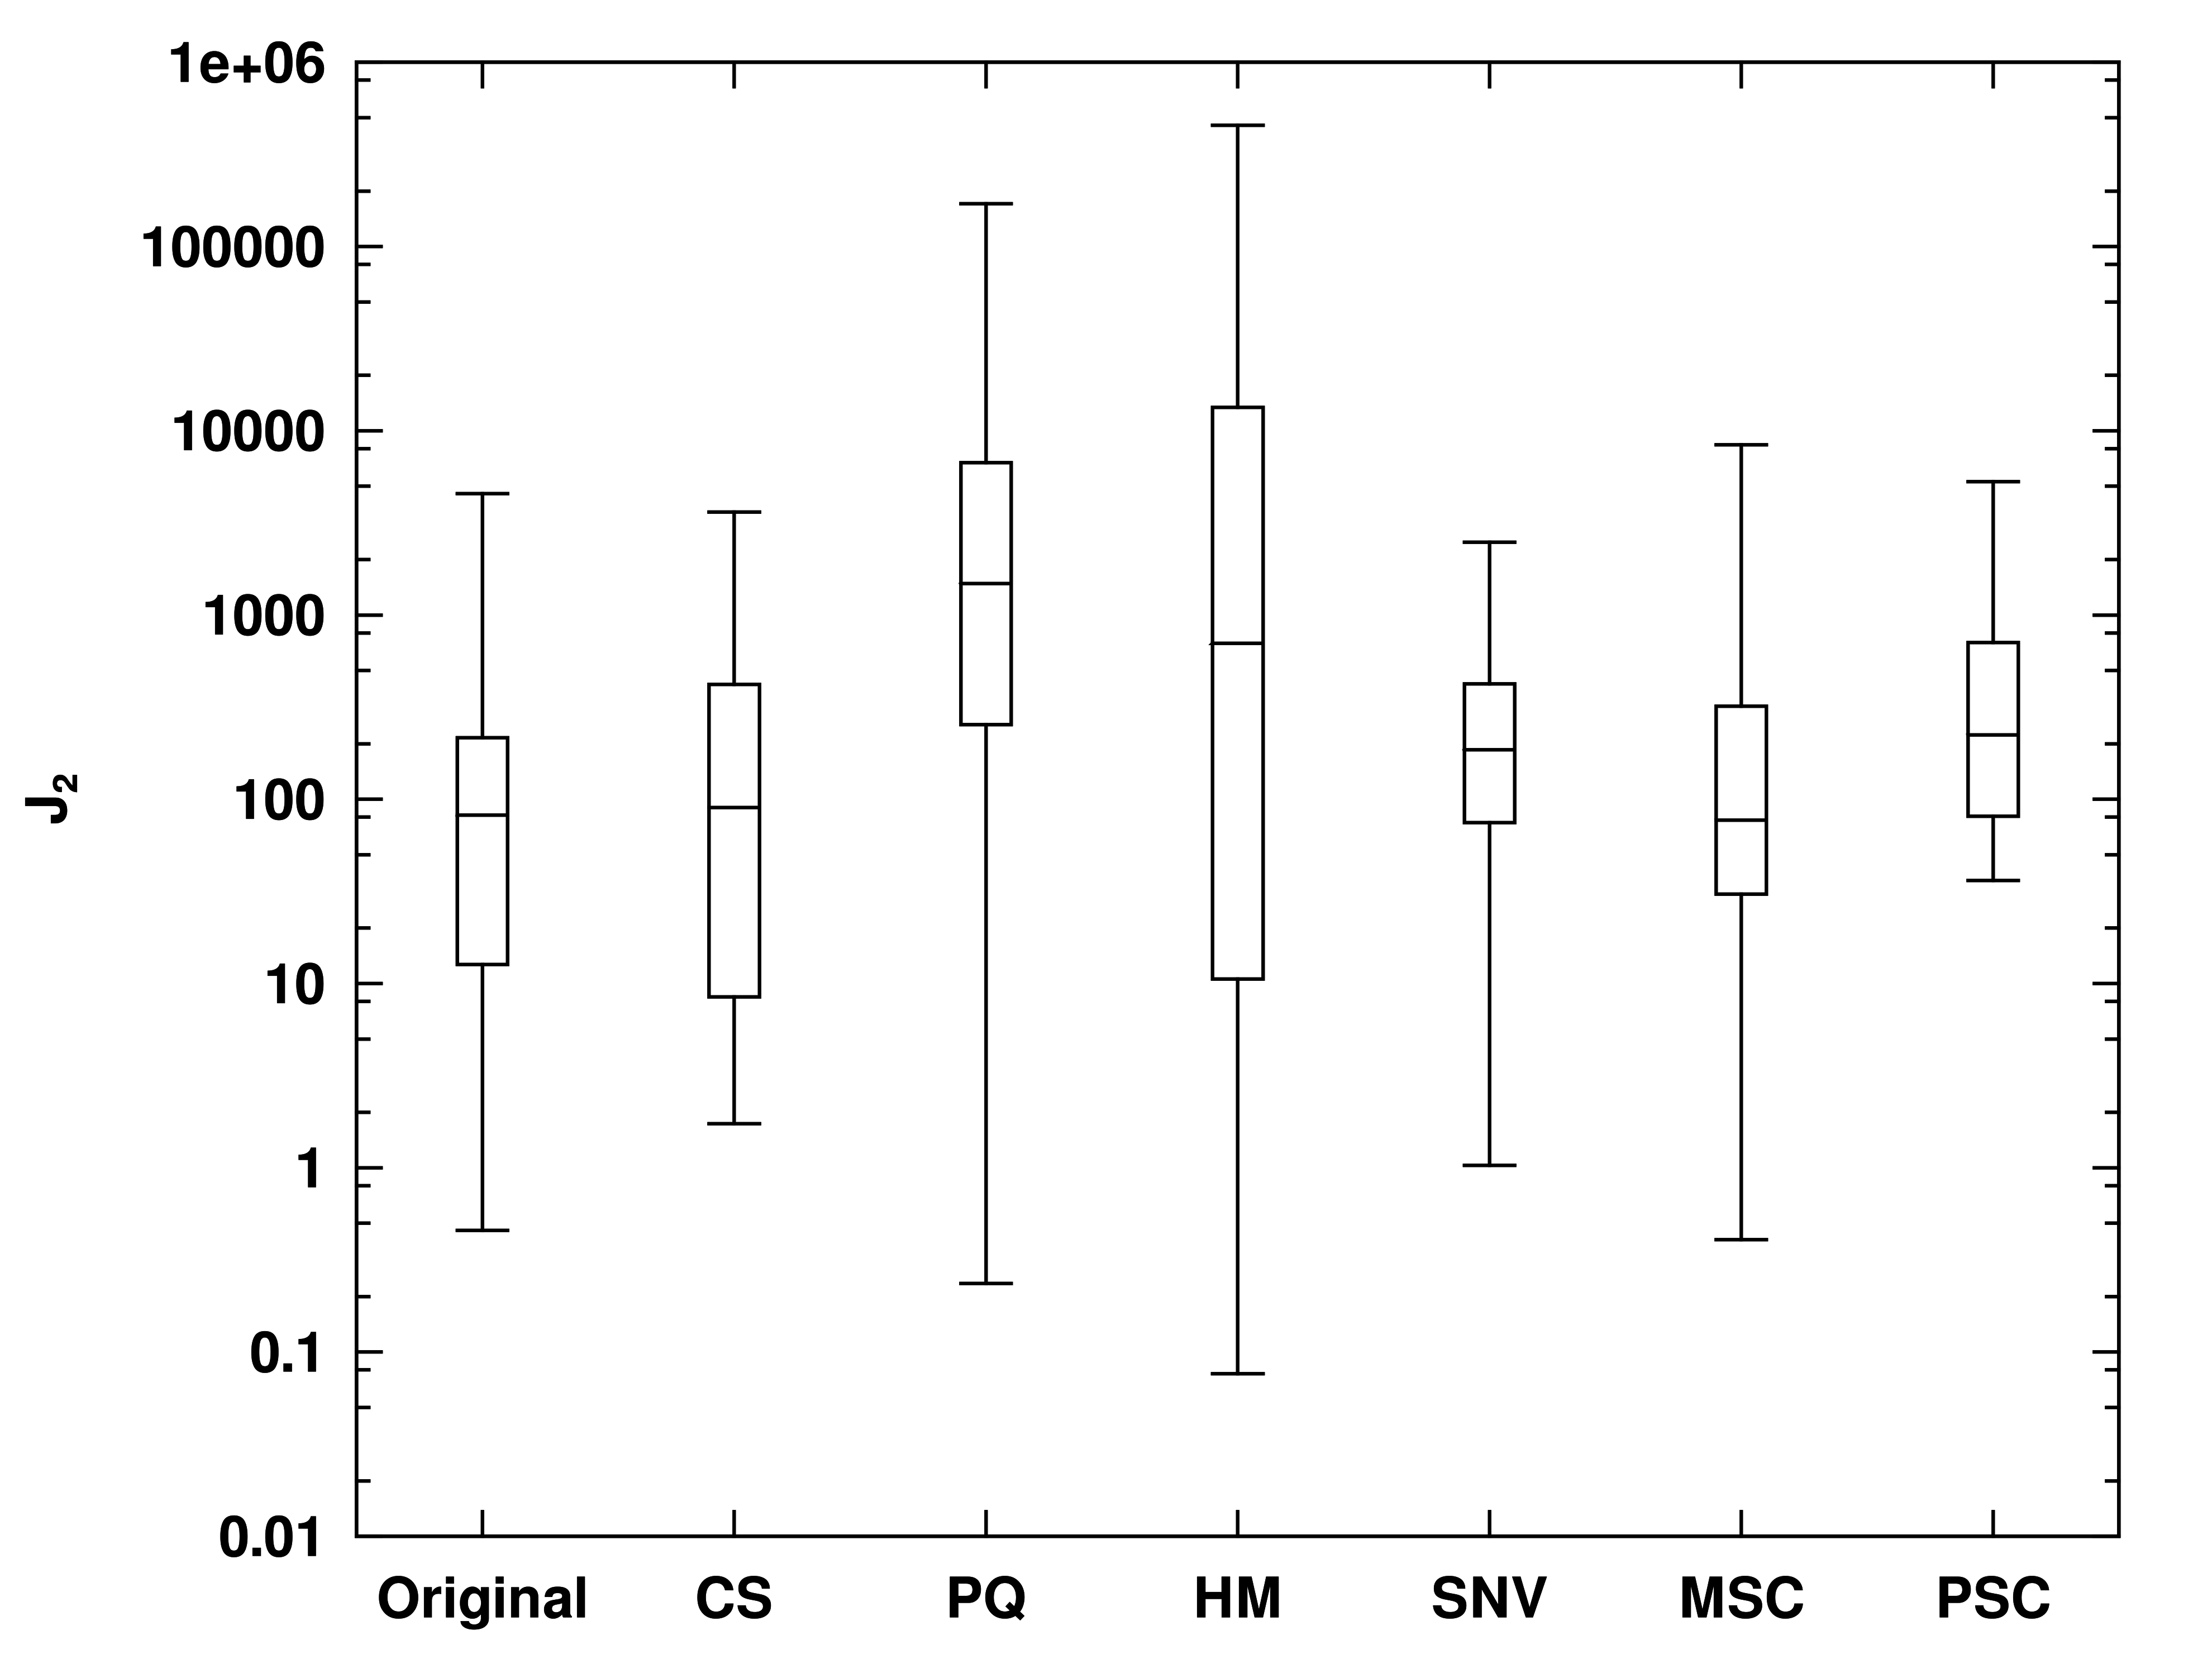
\includegraphics[width=3.5in]{figs/pscorr/02-allj2.png}
\caption
      [Cluster Quality after Normalization and PCA Modeling.]{
  {\bf Cluster Quality after Normalization and PCA Modeling.}
  \\
  Comparison of PCA cluster quality for \hnmr{} NMR metabolomics data
  normalized using different algorithms. For each normalization method, a
  box is defined by the estimated first and third quartiles of $J_2$ for the
  clusters and whiskers are defined by the range of the $J_2$ values for the
  clusters. For this dataset, the minimum $J_2$ value is most instructive,
  given the fact that overall model quality is not well-reflected by the
  $J_2$ metric in the case of distorted principal components.
}
\end{SCfigure}

\begin{doublespace}
To quantify differences between extracted principal components of automatically
and manually phase corrected datasets, the angle between the first principal
component loading vector of each pair of models ($\varphi$) was calculated as
follows:
\begin{equation}
\varphi = \cos^{-1}\left( {\mathbf{p}_{auto}}^T \mathbf{p}_{man} \right)
\end{equation}
where $\mathbf{p}_{auto}$ and $\mathbf{p}_{man}$ are the first-component
loadings computed from a given normalization method's data after automatic
and manual phase correction, respectively. The loading angle $\varphi$ for a
given normalization method is a reflection on that method's ability to properly
normalize data and produce consistent PCA models from different initial phase
error conditions.
\end{doublespace}

\begin{table}[h!]
\caption{Metabolite Spectra Used in Monte Carlo Simulations.}
\begin{center}
\begin{tabular}{l l l l}
  \hline
  Aminobutyrate & Adenosine & Alanine     & Arginine   \\
  Asparagine    & Aspartate & Choline     & Citrulline \\
  Ethanolamine  & Fructose  & Galactose   & Glucose    \\
  Glutamate     & Glutamine & Glycine     & Histidine  \\
  Isoleucine    & Lactate   & Leucine     & Lysine     \\
  Malate        & Maltose   & Myoinositol & Ornithine  \\
  Phenylalanine & Proline   & Putrescine  & Serine     \\
  Succinate     & Sucrose   & Threonine   & Valine
\end{tabular}
\end{center}
\end{table}

\subsection{Simulated NMR Datasets}

\begin{doublespace}
The \hnmr{} NMR spectra of 100 mM samples of 32 metabolites (Table 6.1) at
pH 7.4 were downloaded from the Biological Magnetic Resonance Bank
(BMRB, \cite{ulrich:nar2008}) and fit to mixtures of complex Lorentzian
functions using ACD/1D NMR Processing (Advanced Chemistry Development).
Peak amplitudes ($A$), chemical shifts ($\omega_0$), and widths ($\lambda$)
returned from fitting were loaded into GNU Octave to generate simulated spectra
having 64$k$ data points and a spectral width of 11 ppm, centered at
4.7 ppm, based on the following model function:
\begin{equation}
s(\omega_k) =
 \sum_{p=1}^P
 \frac{A_p \lambda_p}
      {\lambda_p + u_1 (\omega_k - \omega_{0,p})}
\end{equation}
where $s(\omega_k)$ is the $k$-th data point of the spectrum, $P$ equals the
number of peaks, and $u_1$ equals the imaginary unit. Spectra were referenced
and normalized to the DSS peak, and peaks corresponding to HOD and DSS were
subsequently removed, resulting in a basis set of 32 perfectly-phased,
noise-free metabolite spectra. Finally, the basis metabolite spectra were
stored row-wise in a matrix $\mathbf{S}$ for later use in Monte Carlo
calculations.
\end{doublespace}

\begin{figure}[ht!]
\includegraphics[width=6.5in]{figs/pscorr/03-rmse.png}
\caption
      [Monte Carlo Normalization Results.]{
  {\bf Monte Carlo Normalization Results.}
  \\
  Results of 100 Monte Carlo iterations at 0.2$^\circ$ zero-order phase error,
  indicating the ability of all normalization methods to recover the true
  dilution factor of a nearly perfectly phased dataset. Red points reflect the
  dilution factors calculated by integrated the DSS peak and blue points
  reflect the dilution factor estimates from normalization. Upper panels show
  the dilution factors recovered from automatically phased data after
  normalization, and lower panels show dilution factors recovered from
  unphased data after normalization.
}
\end{figure}

\subsection{Monte Carlo Experiments}

\begin{doublespace}
Using the basis metabolite spectra, a dataset of 48 simulated metabolomics
spectra ($\mathbf{X} \in \mathbb{H}_1^{N \times K}$) was generated according
to the following equation:
\begin{equation}
\mathbf{X}
 = \mathbf{A} \left( \mathbf{C} \mathbf{S} + \mathbf{1} \mathbf{r}^T \right)
 + \mathbf{E}
\end{equation}
where $\mathbf{A} \in \mathbb{R}^{N \times N}$ is a diagonal matrix of dilution
factors $\alpha_n$, $\mathbf{C} \in \mathbb{R}^{N \times P}$ is a matrix of
metabolite concentrations, $\mathbf{S} \in \mathbb{H}_1^{P \times K}$ is the
previously created metabolite basis set, $\mathbf{r} \in \mathbb{H}_1^K$ is a
spectrum of the DSS reference peak, $\mathbf{1} \in \mathbb{R}^N$ is a vector
of ones, and $\mathbf{E} \in \mathbb{H}_1^{N \times K}$ is a matrix of complex
Gaussian white noise. Dilution factors were drawn from a log-normal
distribution having zero mean and $\sigma = 0.25$. Concentrations in
$\mathbf{C}$ were drawn from normal distributions with parameters chosen to
mimic those in Torgrip et al. (Table 6.2) \cite{torgrip:metab2008}. The
resultant data in $\mathbf{X}$ is a simulated set of $N = 48$ metabolite
extracts, spiked with 100 $\mu$M DSS, where six distinct classes arise from
differences in the concentrations of alanine, asparagine, glutamate, malate,
proline, sucrose and valine. All other metabolites were assigned concentrations
from a normal distribution having $\mu = 5$ $\mu$M and $\sigma = 0.5$ $\mu$M.
\end{doublespace}

\begin{table}[h!]
\caption{Metabolite Concentrations Altered in Monte Carlo Simulations.}
\begin{center}
\begin{tabular}{l | l l l l l l}
  \hline
  {\bf Metabolite} & $\mathbf{C_A}$ ($\mu$M) & $\mathbf{C_B}$ ($\mu$M) &
                     $\mathbf{C_C}$ ($\mu$M) & $\mathbf{C_D}$ ($\mu$M) &
                     $\mathbf{C_E}$ ($\mu$M) & $\mathbf{C_F}$ ($\mu$M) \\
  \hline
  Alanine    &  $9.2 \pm 1.4$    &  $19.6 \pm 1.6$    &  $16.9 \pm 1.2$  &
                $6.5 \pm 0.66$   &  $26.2 \pm 3.6$    &  $13.5 \pm 1.1$  \\
  Asparagine &  $6.8 \pm 0.86$   &  $11.7 \pm 1.8$    &  $19.0 \pm 1.9$  &
               $14.7 \pm 1.2$    &  $24.8 \pm 2.6$    &  $17.4 \pm 1.0$  \\
  Glutamate  & $13.3 \pm 1.7$    &   $9.2 \pm 1.5$    &  $18.8 \pm 1.9$  &
               $16.9 \pm 2.1$    &  $25.0 \pm 3.5$    &   $6.9 \pm 1.0$  \\
  Malate     & $14.2 \pm 1.2$    &  $11.9 \pm 1.4$    &  $22.0 \pm 5.1$  &
                $6.7 \pm 0.68$   &   $9.4 \pm 0.72$   &  $18.0 \pm 2.4$  \\
  Proline    & $11.4 \pm 1.5$    &  $18.4 \pm 3.1$    &  $14.7 \pm 2.4$  &
                $6.9 \pm 0.62$   &   $9.8 \pm 1.5$    &  $23.7 \pm 2.9$  \\
  Sucrose    &  $7.1 \pm 0.9$    &  $17.2 \pm 2.1$    &  $19.3 \pm 2.0$  &
               $13.2 \pm 1.9$    &   $9.3 \pm 0.56$   &  $23.3 \pm 2.7$  \\
  Valine     &  $9.0 \pm 0.85$   &  $26.3 \pm 2.3$    &  $13.4 \pm 1.2$  &
               $20.4 \pm 1.7$    &   $6.7 \pm 0.90$   &  $17.0 \pm 1.5$  \\
\end{tabular}
\end{center}
\end{table}

\begin{doublespace}
Monte Carlo simulations were run to assess the performance of all discussed
normalization methods over various amounts of phase error added to
$\mathbf{X}$. Forty-six phase error points were calculated, in which the
standard deviation of $\theta_0$ was linearly increased from $0^\circ$ to
$5^\circ$. The standard deviation of $\theta_1$ at each point was equal to
one tenth that of $\theta_0$. Both $\theta_0$ and $\theta_1$ were assigned
zero mean. For each phase error point, 100 Monte Carlo iterations were
performed with different sets of random dilution factors. Spectra in the
de-phased $\mathbf{X}$ matrix were automatically phase corrected using simplex
entropy minimization and normalized each time using CS, PQ, HM, SNV, MSC and
PSC methods. Normalization to unit DSS integral was also performed for
reference. An identical set of normalization calculations was performed on the
unphased data. Estimated dilution factors were compared to the true values
to produce a root-mean-square dilution error, $RMSE(\alpha)$, for each method.
Figure 6.3 shows the $RMSE(\alpha)$ result of Monte Carlo simulation at
$0.2^\circ$ phase error. To assess normalization effects on multivariate model
quality, spectra from each method were uniformly binned with 0.04 ppm bin
widths, each bin scaled to unit variance, and subjected to PCA. Values of
$J_2$ for each of the six classes were then calculated, and the median of the
values was reported for each Monte Carlo iteration. The $\varphi$ values
between automatically phased and unphased principal component loadings were
also calculated at each iteration to asses each normalization method's ability
to produce consistent models in the presence of phase errors. Figure 6.4
summarizes the results of Monte Carlo simulation over all phase errors based
on $RMSE(\alpha)$, $J_2$ and $\varphi$.
\end{doublespace}

\begin{figure}[ht!]
\includegraphics[width=6.5in]{figs/pscorr/04-montecarlo.png}
\caption
      [Summary of Monte Carlo Simulation Results.]{
  {\bf Summary of Monte Carlo Simulation Results.}
  \\
  Results of the Monte Carlo simulation over all phase error points.
  ({\bf A}) As phase error increases, dilution factor estimates from all
  methods except PQ remain fairly stable. Estimates from PSC compete with
  MSC, but suffer in comparison with HM.
  ({\bf B}) However, $J_2$ values indicate that PSC outperforms all other
  normalization methods at producing tight clusters at any realistic
  phase error.
  ({\bf C}) Finally, values of $\varphi$ calculated from PCA loadings indicate
  that PSC maintains the highest model consistency in the face of imperfectly
  phased data. Phase error on the $x$-axis refers to zero-order error; it
  should be noted that each point also contains first-order phase error as
  discussed in the Methods.
}
\end{figure}

\section{Results}

\begin{doublespace}
FIXME.
\end{doublespace}

\section{Discussion}

\begin{doublespace}
FIXME.
\end{doublespace}

\section{Conclusions}

\begin{doublespace}
FIXME.
\end{doublespace}

\bibliographystyle{abbrv}
\bibliography{bworley}



\chapter{Generalized Adaptive Intelligent Binning of Multiway Data}

\begin{quote}
{\it
  The art of doing mathematics consists in finding that special case which
  contains all the germs of generality.}
\\\\
 -- David Hilbert
\end{quote}

\section{Introduction}

\begin{figure}[hb!]
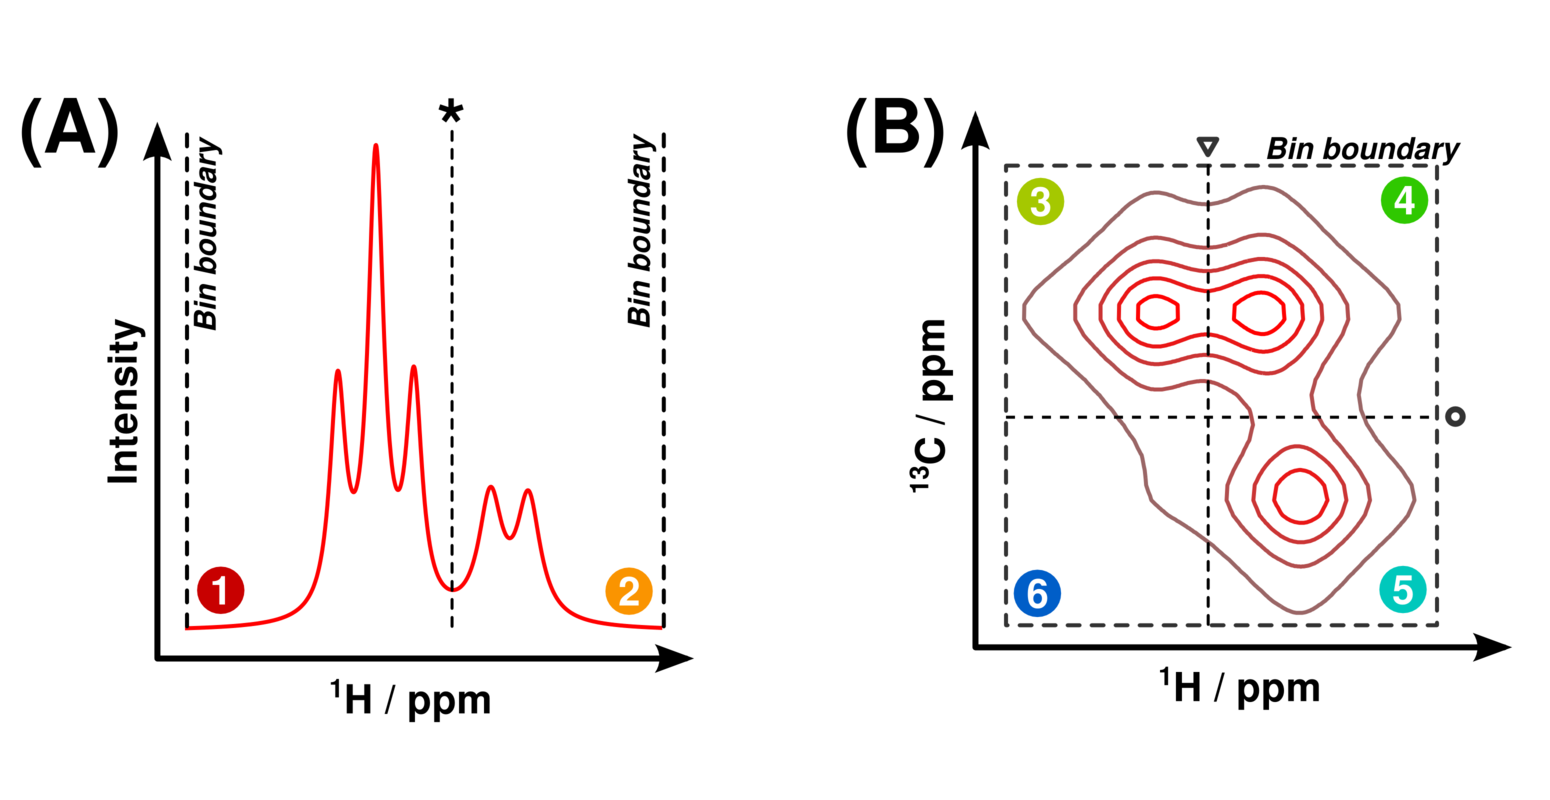
\includegraphics[width=6.5in]{figs/gaibin/01.png}
\caption
      [Generalization of Adaptive Intelligent Binning.]{
  {\bf Generalization of Adaptive Intelligent Binning.}
  \\
  ({\bf A}) In the one-dimensional case, the bin containing regions 1 and 2
  is optimally subdivided ({\it asterisk}) when the sum of the objective values
  in regions 1 and 2 is maximal and greater than the original bin's objective
  value. ({\bf B}) In the $D$-dimensional case, there are now $D$ possible
  dimensions along which an optimal subdivision may exist. The optimal
  subdivision along the \hnmr{} dimension ({\it triangle}) occurs when the sum
  of the objective values in regions 3+6 and 4+5 is maximal and greater than
  that of the original bin. Similarly, the optimal subdivision along the
  \cnmr{} dimension ({\it circle}) occurs when the sum of the objective values
  in regions 3+4 and 5+6 is maximal and above the original bin objective. A
  comparison between all possible optimal subdivisions along all dimensions
  yields the best possible subdivision (\cnmr{}, {\it circle}).
}
\end{figure}

\begin{doublespace}
By and large, the phase ``NMR metabolic fingerprinting'' implies the use of
one-dimensional (1D) \hnmr{} NMR spectroscopic methods, due in no small part
to the ease and speed of 1D data collection and the large natural abundance
of NMR-active protons found in metabolomics samples
\cite{lindon:cmr2000,worley:cmb2013}. Before processed spectra are
submitted to PCA or PLS for modeling, they are often subdivided into bins
to simplify multivariate analyses. Spectral binning, introduced and described
in detail in \hyperlink{chapter.3}{Chapter 3}, reduces the dimensionality of
a data matrix and masks chemical shift variability between samples at the
expense of decreased model interpretability: any given bin in a 1D \hnmr{} NMR
spectral dataset may contain several overlapped signals from multiple distinct
metabolites \cite{aberg:abc2009}. Thus, without utilizing
computationally intensive methods of deconvolution to tease apart signal
contributions from individual metabolites
\cite{astle:jasa2012,zheng:binf2011}, the resulting fingerprint from a
binned 1D dataset is usually limited to high-level inference about metabolic
trends.
\\\\
By leveraging the connectivities between \hnmr{} and \cnmr{} nuclei in
metabolites, two-dimensional (2D) heteronuclear NMR methods reduce spectral
overlap by spreading \hnmr{} information over a second (\cnmr) chemical shift
dimension \cite{mandal:cmr2004}. Heteronuclear single quantum coherence (HSQC)
experiments are commonly performed in NMR metabolic profiling studies, and
provide an NMR singlet or multiplet for each directly bonded \hcnmr{} pair
in the sample. Developments in NMR hardware and acquisition techniques have
brought natural abundance \hcnmr{} HSQC experiment times down to values
compatible with high-throughput metabolic fingerprinting studies
\cite{motta:anchem2010,rai:anchem2012}. However, multivariate analysis
of 2D NMR datasets is still a nontrivial undertaking that requires either
vectorization \cite{hedenstrom:cils2008}, which breaks the inherent
structure of the data, or the use of multilinear factorizations
\cite{lu:ieee2009,lu:pr2011}, which are more computationally intensive
and difficult to cross-validate.
\\\\
Spectral binning is another potential means of preparing 2D NMR datasets for
multivariate analysis that holds several advantages over binning 1D spectra.
First, multiple integration of bins maps each spectrum to an observation
vector regardless of its original dimensionality, allowing bilinear PCA and
PLS algorithms to be used without concern for loss of the inherent structure
of the data. Second, binning of 2D spectral data yields more well-conditioned
data matrices than simple vectorization. Finally, because signals are better
resolved in 2D spectra, each bin contains substantially fewer signals from
distinct metabolites. Multiple different algorithms have been developed to
bin 1D NMR data \cite{
  anderson:metab2008,
  anderson:metab2011,
  davis:cils2007,
  demeyer:anchem2008,
  sousa:cils2013}, and the use of uniform binning on 2D NMR data has also been
reported \cite{van:jpr2008}. However, to our knowledge, no methods
exist to {\it intelligently} bin multidimensional data for use in multivariate
analyses. This motivated the development of a generalization of Adaptive
Intelligent (AI) binning \cite{demeyer:anchem2008} to spectral data
of any dimensionality, called Generalized Adaptive Intelligent (GAI) binning
(Figure 6.1).
\end{doublespace}

\section{Theory}

\subsection{AI-binning}

\begin{doublespace}
Generalized AI-binning (GAI-binning) is a logical extension of AI-binning to
two or more dimensions. In the AI algorithm (Figure 6.1A), bins are recursively
subdivided until a stopping criterion or minimum bin width is reached
\cite{demeyer:anchem2008}. For a 1D dataset containing $N$ spectra,
the following objective function is used to assess the quality of each bin:

\begin{equation}
V_b = \frac{1}{N}
  \sum_{n=1}^N \left[
    (max_{n,b} - I_{n,b,1})
    (max_{n,b} - I_{n,b,end}) \right]^\frac{R}{2}
\end{equation}

where $max_{n,b}$ is the maximum intensity inside the bin $b$ in spectrum $n$,
and $I_{n,b,1}$ and $I_{n,b,end}$ are the bin edge intensities. The exponent
$R$ in the AI objective function is referred to as a `resolution parameter',
which offers a means of tuning the binning result based on signal-to-noise and
peak resolution of a dataset. The replacement of $R$ with $\frac{R}{2}$ in the
exponent of equation 6.1, enables a slightly modified interpretation of each
summed term in the AI objective function as a relaxed form of a geometric mean
of the differences between the bin edge intensities and the maximum bin
intensity. At each subdivision step, new bin edges are chosen to maximize the
combined (summed) objective values of the two resulting bins over the objective
value of the original bin. If no bin subdivision exists with a combined
objective value greater than that of the original bin, recursive subdivision
within that bin is terminated, and the AI algorithm terminates once all bins
may no longer be subdivided.
\end{doublespace}

\subsection{GAI-binning}

\begin{doublespace}
In two or more dimensions, the set of bin boundary points expands to include
all points that lie on the edges (or faces, hyperfaces, {\it etc.}) of the bin.
By denoting the set of all edge points in bin $b$ as $E_b$, a new objective
function may be constructed:

\begin{equation}
V_b = \frac{1}{N}
  \sum_{n=1}^N \left[
    \prod_{e \in E_b} (max_{n,b} - I_e)
  \right]^\frac{R}{||E_b||}
\end{equation}

Thus, the GAI algorithm computes the `relaxed' geometric mean of the
differences between the bin maximum and all points on the boundary. In the
case of one-dimensional data, it is apparent that equation 6.2 reduces to
equation 6.1, and GAI-binning operates identically to AI-binning. As
dimensionality increases, the risk of floating-point overflow or underflow
increases due to the larger bin edge set $E_b$. To avoid this, the following
`log-objective' may be used in lieu of equation 6.2:

\begin{equation}
V_{b,ln} = \frac{R}{N ||E_b||}
  \sum_{n=1}^N \sum_{e \in E_b}
    \ln(max_{n,b} - I_e)
\end{equation}

Like AI-binning, GAI-binning initializes a bin around the entire dataset and
proceeds to recursively subdivide each bin until a minimum bin size is reached
or no bin may be divided to yield an increase in the objective value. Because
the number of ways to subdivide each bin increases with dimensionality, all
possible dimensions are tested, and the new bin boundary that maximizes the
objective over all possible subdivision dimensions is selected (Figure 6.1B).
Therefore, the GAI algorithm may be considered a form of binary space
partitioning (BSP) which limits its partition hyperplanes to lying orthogonally
to the basis vectors of the coordinate system \cite{deberg2000}.
\end{doublespace}

\subsection{Noise Bin Elimination}

\begin{doublespace}
It is important that noise bins be removed from the data matrix prior to
multivariate analysis, as their presence is known to negatively impact the
interpretability and reliability of multivariate models
\cite{halouska:jmr2006,bro:anmeth2014}. Because the integration of a
noisy space of increasing dimensionality ({\it i.e.} double or triple
integration) results in a random variable having a similarly increasing
variance, the importance of noise removal is compounded in multidimensional
binning. Therefore, a noise bin removal step based on spectral intensity was
added to the GAI algorithm. A running mean and variance calculation was
performed to estimate the noise floor of each spectrum. The initial mean
$\mu_n$ and standard deviation $\sigma_n$ of the noise were computed using the
first 32 points on one edge of the spectrum, which were assumed to contain only
baseline noise. Every other data point was then classified as signal or noise
based on whether its intensity exceeded the current running noise floor,
$\mu_n + 3 \sigma_n$. Upon inclusion of a new noise data point, the mean and
standard deviation of the noise were appropriately updated. Once the estimated
noise floor was determined for each spectrum in the dataset, a threshold for
bin removal was computed as the median noise floor of all the spectra:

\begin{equation}
I_{th} = \mathrm{med}_n (\mu_n + k \sigma_n)
\end{equation}

where $k$ is a user-selectable parameter to adjust the noise threshold. Only
bins whose maximum intensity fell above $I_{th}$ were retained in the final
data matrix.
\end{doublespace}

\section{Materials and Methods}

\subsection{Human Liver Dataset}

\begin{doublespace}
Two independently collected \hcnmr{} HSQC NMR datasets from ongoing
metabolomics studies were used as test cases for the GAI-binning algorithm.
For the first dataset, twenty-four 1.0 mL samples of SK-Hep1 human liver cells
were provided for metabolic fingerprinting, half of which were treated with
50 $\mu$M tetrathiomolybdate (TTM). The cells were extracted into 80:20
methanol:water to collect the water-soluble metabolites, spun in a rotary
evaporator for two hours, lyophilized at -50 $^\circ$C and 0.02 mBar for 24
hours, and finally redissolved in 600 $\mu$L of 50.0 mM phosphate buffer in
99.8\% D$_2$O (Isotec, St. Louis, MO) adjusted to pH 7.4. The redissolved,
pH-adjusted samples were then collected into NMR tubes.
\\\\
Experiments were collected on a Bruker Avance III HD 700 MHz spectrometer
equipped with a 5 mm inverse quadruple-resonance (\hnmr{}, \cnmr{}, \nnmr{},
\pnmr{}) cryoprobe with cooled \hnmr{} and \cnmr{} channels and a {\it z}-axis
gradient. A Bruker SampleJet and ICON-NMR were used to automate NMR data
collection. A 2D gradient-enhanced \hcnmr{} HSQC with improved sensitivity
\cite{palmer:jmr1991,kay:jacs1992} ({\it hsqcetgpsi}) was collected for
each sample. Spectra were collected with 4 scans and 16 dummy scans over a
uniform Nyquist grid of 512 and 64 complex points along the \hnmr{} and \cnmr{}
dimensions, respectively. Spectral windows were set to 3,285 $\pm$ 4,545 Hz
along \hnmr{} and 12,677 $\pm$ 14,620 Hz along \cnmr{}. All spectra were
collected at a sample temperature of 298.0 K.
\end{doublespace}

\begin{figure}[hb!]
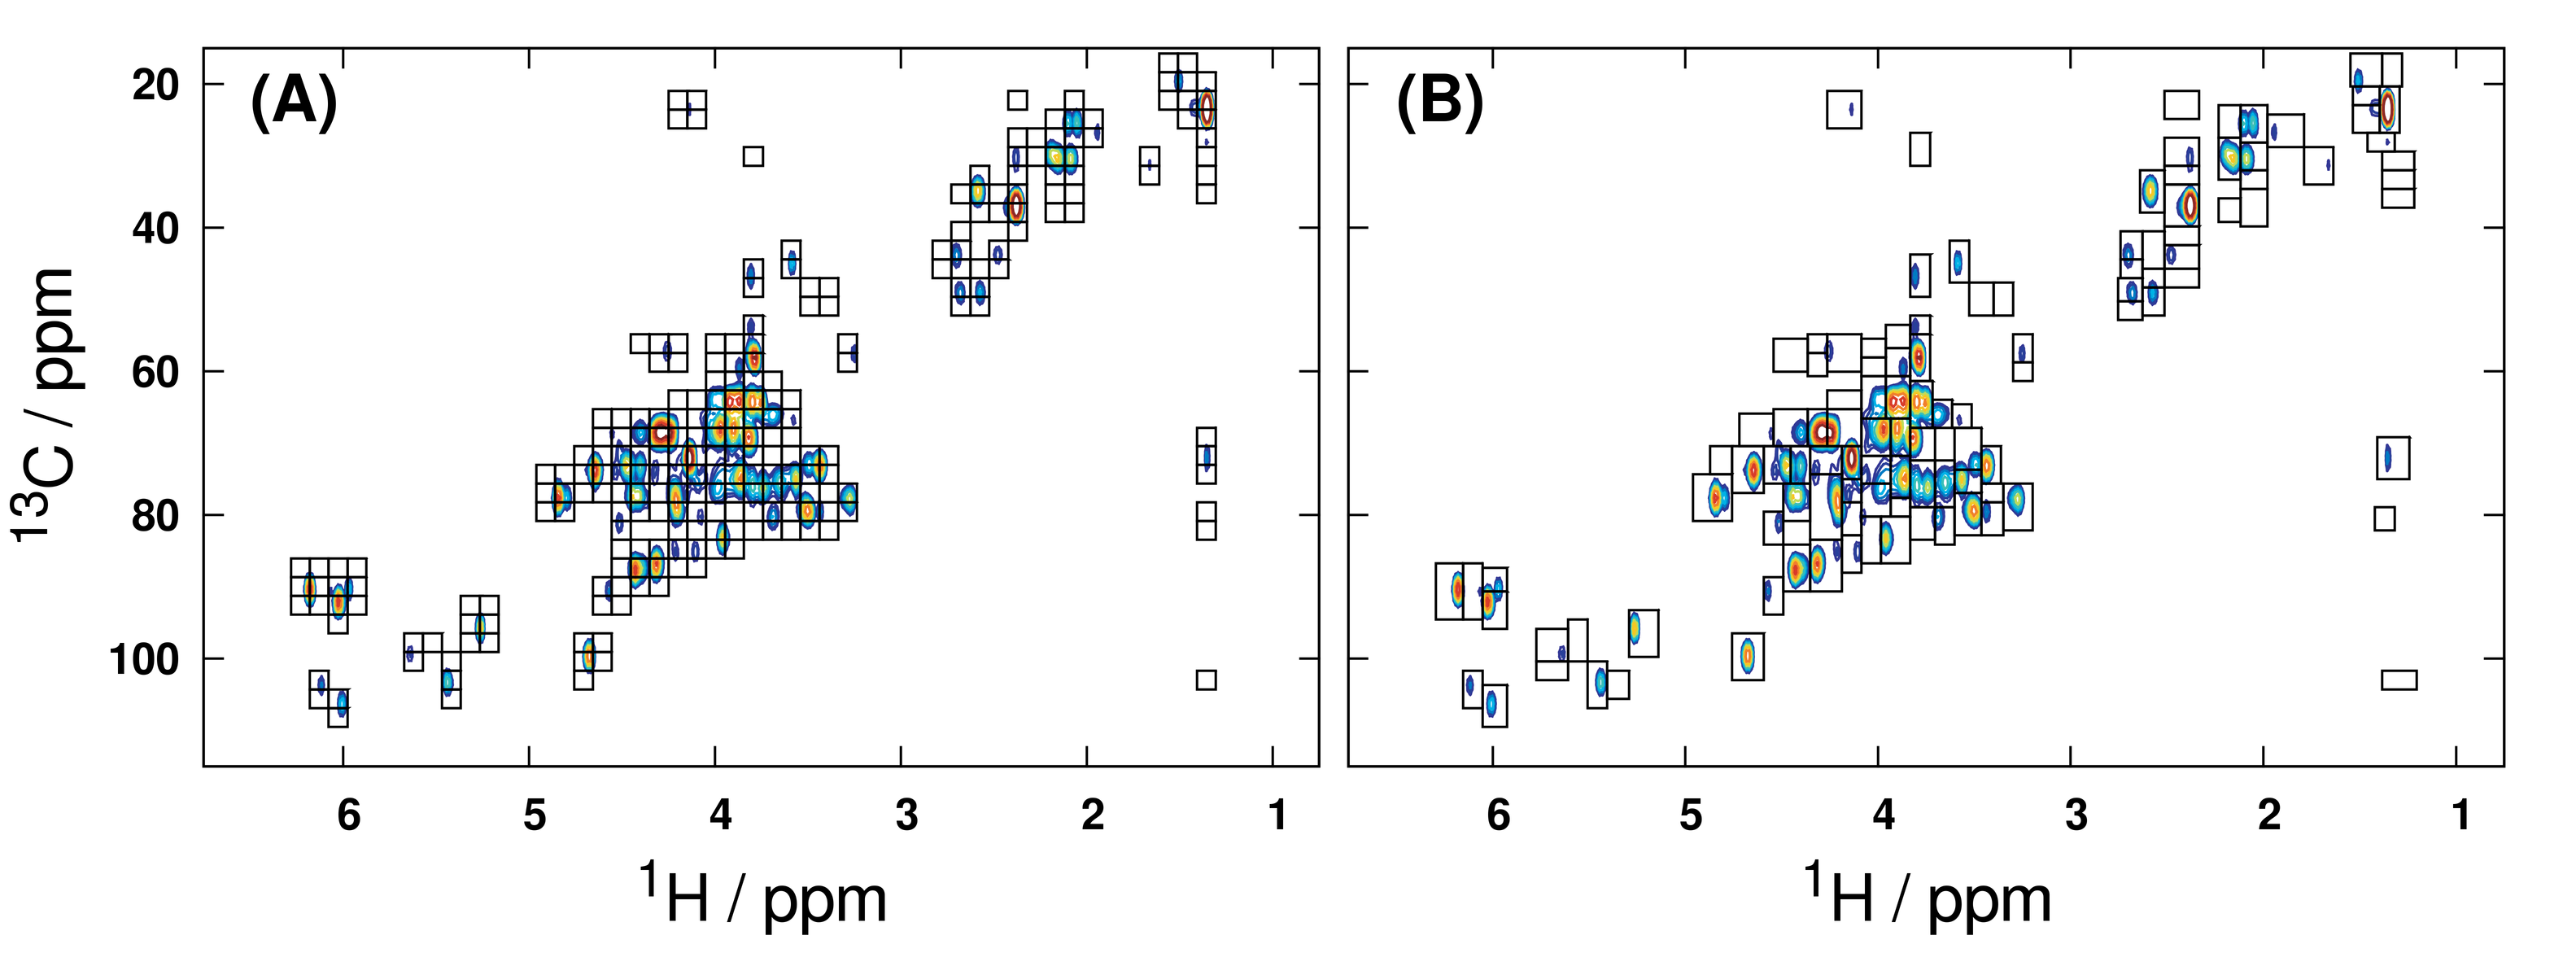
\includegraphics[width=6.5in]{figs/gaibin/02.png}
\caption
      [Binned Liver Dataset.]{
  {\bf Binned Liver Dataset.}
  \\
  Processed \hcnmr{} HSQC mean spectrum of the liver data tensor, with
  overlaid uniform ({\bf A}) and GAI ({\bf B}) bin boundaries.
}
\end{figure}

\subsection{Mouse Embryonic Fibroblast Dataset}

\begin{doublespace}
A second set of samples from kinase suppressor of Ras 1 (KSR1) knockout mouse
embryonic fibroblast (MEF) cells was also provided to generate a test
\hcnmr{} HSQC dataset for GAI-binning. For this second dataset, ten cell
samples from $ksr^{-/-}$ MEFs and ten samples from KSR1-rescued $ksr^{-/-}$
MEFs were used to produce metabolite extracts. The cells were washed, extracted
into 80:20 methanol:water, spun in a rotary evaporator, lyophilized and
redissolved according to the procedures used to extract metabolites from the
liver cell samples.
\\\\
Experiments were collected on a Bruker Avance DRX 500 MHz spectrometer equipped
with a 5 mm inverse triple-resonance (\hnmr{}, \cnmr{}, \nnmr{}) cryoprobe with
a {\it z}-axis gradient. A Bruker BACS-120 sample changer and ICON-NMR software
were used to automate data collection. A 2D gradient-enhanced \hcnmr{}
HSQC ({\it hsqcetgp}) was collected for each sample. Spectra were collected
with 128 scans and 16 dummy scans over a uniform grid of 1024 and 32 complex
points along the \hnmr{} and \cnmr{} dimensions, respectively. Spectral windows
were set to 2,359 $\pm$ 2,367 Hz along \hnmr{} and 8,174 $\pm$ 8,803 Hz along
\cnmr{}. All spectra were collected at a sample temperature of 293 K.
\end{doublespace}

\begin{figure}[ht!]
\includegraphics[width=6.5in]{figs/gaibin/03.png}
\caption
      [Binned Fibroblast Dataset.]{
  {\bf Binned Fibroblast Dataset.}
  \\
  Processed \hcnmr{} HSQC mean spectrum of the MEF data tensor, with
  overlaid uniform ({\bf A}) and GAI ({\bf B}) bin boundaries.
}
\end{figure}

\subsection{NMR Processing and Multivariate Analysis}

\begin{doublespace}
All processing, treatment and statistical modeling were performed in GNU Octave
3.6 \cite{eaton2008} using routines currently available in the MVAPACK
toolbox for NMR chemometrics \cite{worley:acscb2014}, discussed in
\hyperlink{chapter.4}{Chapter 4}. The 2D raw serial files were loaded
\cite{delaglio:jbnmr1995}, apodized with a squared-sine window,
zero-filled once along \hnmr{} and twice along \cnmr{}, and
Fourier-transformed. Spectra from the liver cell extracts were manuall
phase-corrected and cropped (1.0 -- 6.6 ppm along \hnmr{}; 16 -- 112 ppm
along \cnmr{}), and spectra from the MEF extracts were similarly phase
corrected and cropped (1.25 -- 6.2 ppm along \hnmr{}; 8 -- 102 ppm
along \cnmr{}). Both uniform and GAI-binning were performed on each data tensor
using minimum \hnmr{} and \cnmr{} bin widths of 0.025 and 2.5
ppm, respectively, and a GAI resolution parameter of 0.1. Binned regions
identified to be less intense than three times the standard deviation of the
spectral noise ($k = 3$) were removed after binning. The mean spectra of the
entire processed liver and MEF datasets, superimposed with bins identified by
both uniform and GAI-binning, are shown in Figure 6.2 and Figure 6.3.
\\\\
The applicability of GAI-binning to bilinear factorizations was demonstrated
by modeling the data tensors using both PCA and OPLS-DA. For PCA modeling of
the data, the spectral regions identified by each binning method were doubly
integrated. Scores and loadings were then calculated using the Nonlinear
Iterative Partial Least Squares (NIPALS) algorithm
\cite{jolliffe2002}. Internal leave-one-out cross-validation (LOOCV)
of each computed PCA model was performed to yield model fit (\rsqx{}) and
predictive ability (\qsq{}) statistics
\cite{krzanowski:biom1987,eshghi:cils2014}. For OPLS-DA, spectral data
points within the identified bins were vectorized row-wise into a data matrix
as previously described \cite{hedenstrom:cils2008}. During
vectorization, all data points within each binned region are stacked into an
observation vector, and data points not within bins are excluded. The use of
vectorization prior to supervised modeling facilitates the creation of
backscaled pseudospectral OPLS loadings, which hold greater ease of
interpretation over binned loadings \cite{wiklund:anchem2008}.
Modeling by an OSC-filtered NIPALS algorithm
\cite{trygg:jchemo2002} and 100 rounds of seven-fold Monte Carlo
cross-validation (MCCV) \cite{xu:jchemo2004} were performed to
compute data fit (\rsqx{}), response fit (\rsqy{}) and model predictive ability
(\qsq{}) statistics. The binned data matrices produced via double integration
were also subjected to OPLS-DA modeling in the same manner as the vectorized
data. All OPLS-DA models were further validated using CV-ANOVA
\cite{eriksson:jchemo2008} and 1,000 iterations of response
permutation testing \cite{westerhuis:metab2008a} to rigorously ensure
model reliability. Backscaled predictive OPLS loadings were computed from the
vectorized bins according to previously published works
\cite{cloarec:anchem2005a,hedenstrom:cils2008}. During backscaling,
OPLS loading vectors were scaled by the inverse of their original Pareto
scaling coefficients and then unstacked into a two-dimensional pseudospectrum
using bin information. Data points not included in the vectorized loadings were
set to zero in the backscaled pseudospectrum. All data matrices were normalized
using Probabilistic Quotients (PQ) \cite{dieterle:anchem2006} and then
Pareto scaled \cite{vandenberg:bmcg2006} prior to modeling.
\end{doublespace}

\section{Results and Discussion}

\begin{doublespace}
Processing of the liver extract spectra yielded a real data tensor of 24
\hcnmr{} HSQC spectra having 442$\times$149 points each, and processing of the
fibroblast spectra yielded a tensor of 17 spectra having 1,071$\times$172
real data points each. The observation counts ($N$), variable counts ($K$)
and PCA/OPLS cross-validation statistics (\rsq{}, \qsq{}) for each dataset and
variable reduction method are summarized in Table 6.1. Further validation
results from the OPLS models, all of which indicate varying degrees of high
model reliability, are also summarized in Table 6.2. Through examination of the
variable counts within Table 6.1, it is readily apparent that GAI-binning is
dramatically more effective than uniform binning at discriminating between
signal and noise regions within spectral data. On average, GAI-binning
segmented each data tensor into less than half the number of bins produced by
uniform binning, and produced PCA models with markedly higher \rsqx{} and
\qsq{} statistics. Moreover, even with the greatly reduced variable counts
produced by GAI-binning relative to uniform binning, the OPLS \qsq{} statistics
between the two methods are statistically indistinguishable. In fact, the
variable counts resulting from GAI-binning these third-order tensors are
substantially lower than the few hundred variables typically produced by
binning {\it one}-dimensional spectra. Resulting scores from PCA modeling
of the GAI-binned liver data tensor are shown in Figure 6.4.
\end{doublespace}

\begin{table}[h!]
\caption{Data Matrices and PCA/OPLS Model Statistics.}
\begin{center}
\begin{tabular}{l l | l l l l l | l l l}
  \hline
              &         &
    \multicolumn{5}{c|}{{\bf Integration}} &
    \multicolumn{3}{c}{{\bf Vectorization}} \\
              &         &
    \multicolumn{3}{c}{PCA} &
    \multicolumn{2}{c|}{OPLS} & &
    \multicolumn{2}{c}{OPLS} \\
  \hline
              &         &
    $K$       & \rsqx{} & \qsq{} & \rsqy{} & \qsq{} &
    $K$                          & \rsqy{} & \qsq{} \\
  \hline
  {\bf Liver} & Unif.   &
    248       & 0.82    & 0.71   & 0.993   & 0.938 $\pm$ 0.002 &
    11,160                       & 0.993   & 0.929 $\pm$ 0.003 \\
  $N = 24$    & GAI     &
    113       & 0.89    & 0.75   & 0.991   & 0.928 $\pm$ 0.003 &
    10,474                       & 0.994   & 0.933 $\pm$ 0.003 \\
  \hline
  {\bf MEF}   & Unif.   &
    334       & 0.48    & 0.40   & 0.994   & 0.974 $\pm$ 0.004 &
    18,348                       & 0.994   & 0.963 $\pm$ 0.005 \\
  $N = 17$    & GAI     &
    93        & 0.71    & 0.56   & 0.994   & 0.973 $\pm$ 0.005 &
    18,789                       & 0.996   & 0.962 $\pm$ 0.006
\end{tabular}
\end{center}
\end{table}

\begin{table}[h!]
\caption{OPLS-DA Cross Validation $p$-values.}
\begin{center}
\begin{tabular}{l l | l l | l l}
  \hline
              &       &
    \multicolumn{2}{c|}{{\bf Integration}} &
    \multicolumn{2}{c}{{\bf Vectorization}} \\
              &       & Permutation & CV-ANOVA & Permutation & CV-ANOVA \\
  \hline
  {\bf Liver} & Unif. &
    $< 0.001$ & $3.24 \times 10^{-11}$ & $< 0.001$ & $4.70 \times 10^{-11}$ \\
  $N = 24$    & GAI   &
    $< 0.001$ & $3.34 \times 10^{-10}$ & $< 0.001$ & $9.74 \times 10^{-11}$ \\
  \hline
  {\bf MEF}   & Unif. &
    $< 0.001$ & $3.56 \times 10^{-10}$ & $< 0.001$ & $1.73 \times 10^{-9}$ \\
  $N = 24$    & GAI   &
    $< 0.001$ & $1.37 \times 10^{-9}$  & $< 0.001$ & $2.34 \times 10^{-9}$
\end{tabular}
\end{center}
\end{table}

\begin{SCfigure}
\includegraphics[width=3.5in]{figs/gaibin/04.png}
\caption
      [PCA Scores of a GAI-binned Tensor.]{
  {\bf PCA Scores of a GAI-binned Tensor.}
  \\
  Principal component analysis scores resulting from modeling the GAI-binned
  \hcnmr{} HSQC liver data matrix, indicating a high degree of separation
  between experimental groups. Model \rsqx{} and \qsq{} were 0.68 and 0.64 for
  the first principal component ($t_1$) and 0.12 and 0.09 for the second
  ($t_2$). Class separations of this magnitude are readily achievable using
  data matrices generated by GAI-binning, due in large part to the low variable
  counts it generally produces.
}
\end{SCfigure}

\begin{doublespace}
Backscaled predictive OPLS-DA loadings of the vectorized \hcnmr{} HSQC spectral
data tensors (Figure 6.5) lend further support for the use of multidimensional
binning in metabolic fingerprinting studies. Even when vectorization is
performed in place of integration to produce a data matrix, binning offers an
effective means of variable selection: only 10,474 of 65,858 variables (16\%)
were retained when GAI-binning was used as a pre-filter prior to modeling the
liver data. A similar reduction was observed in the fibroblast dataset, where
GAI-binning retained 18,789 of 184,212 total variables for a 90\% reduction in
dimensionality. These substantially reduced variable counts offered by binning
translate to more well-conditioned bilinear modeling problems. As the
dimensionality of the input dataset is increased further, the reductions in
variable count afforded by multidimensional binning are expected to become even
more dramatic. While the variable counts produced by vectorization of uniformly
binned data tensors are comparable to those from GAI-binning, it is critical to
recognize that the uniformly binned regions contain more noise data points than
their GAI-binned counterparts, and thus offer a less efficient dimensionality
reduction.
\\\\
Spectral regions produced by GAI-binning (Figure 6.2) demonstrate several
important properties of the combined binning and noise removal processes.
Because $t_1$ noise and truncation artifacts yield phase-incoherent negative
spectral excursions after Fourier transformation, `unrelaxed' GAI-binning
($R = 1$) tends to preferentially subdivide near such regions, producing
elongated bins along the $F_1$ dimension. Decreasing the resolution parameter
from its maximum value shrinks these bins to contain only true signals. Thus,
an objective rule for determining an optimal resolution parameter during
binning is to decrease $R$ until all bins shrink to contain a minimal amount
of noise. Once an optimal resolution parameter has been identified, a suitable
noise threshold ($k$) must be determined such that all noise bins are removed
without loss of bins containing weak signals. However, once $R$ and $k$ have
been determined for a given set of experimental conditions, they may be applied
during GAI-binning to any data collected at later times under the same
conditions to achieve ideal results. The selections of resolution parameter
($R = 0.1$) and noise threshold ($k = 3$) made in this work were identified
according to the above criteria through a manual visual examination of the
binning results, but it is conceivable that objective metrics of these criteria
could be constructed that facilitate automated determination of these
parameters.
\\\\
Finally, like AI-binning, the execution time of GAI-binning scales
quadratically with the number of spectral data points, and scales approximately
linearly with both the number of spectral dimensions and the number of
observations. Typical runtimes for binning two-dimensional datasets range from
seconds to a few minutes, depending mostly on the data point count. Thus,
while zero-filling may be used to increase the digital resolution of data
being input into GAI-binning, it should be applied sparingly to avoid
unnecessarily long computation times during bin region determination.
\end{doublespace}

\begin{figure}[hb!]
\includegraphics[width=6.5in]{figs/gaibin/05.png}
\caption
      [Pseudospectral HSQC Loadings.]{
  {\bf Pseudospectral HSQC Loadings.}
  \\
  Backscaled full-resolution pseudospectral loadings from OPLS-DA modeling of
  the GAI-reduced ({\bf A}) liver and ({\bf B}) fibroblast \hcnmr{} HSQC data
  tensors. Positive and negative loadings are represented by red and blue
  contours, respectively.
}
\end{figure}

\section{Conclusions}

\begin{doublespace}
Generalized Adaptive Intelligent binning is a logical extension of the
previously described Adaptive Intelligent binning algorithm
\cite{demeyer:anchem2008} to multidimensional datasets, and provides a
model-free alternative to peak-fitting and peak-picking as a means of variable
selection in multivariate analyses. Furthermore, GAI-binning is a more
intelligent method to extract signal regions from multidimensional spectral
data tensors than uniform binning, and may be used to generate very
low-dimensionality data matrices via multiple integration or efficiently
noise-filtered data matrices via vectorization. The C++ implementations of
1D and 2D GAI-binning used in this work are freely available as part of the
MVAPACK software package \cite{worley:acscb2014} introduced in
\hyperlink{chapter.4}{Chapter 4}.
\end{doublespace}

\section{Permutation Test Results}

\begin{figure}[ht!]
\includegraphics[width=6.5in]{figs/gaibin/06.png}
\caption
      [Response Permutation Test: Uniform integration.]{
  {\bf Response Permutation Test: Uniform integration.}
  \\
  Response permutation test results for OPLS-DA models from the uniformly
  binned (integrated) liver ({\bf A}, {\bf B}) and fibroblast
  ({\bf C}, {\bf D}) data tensors. Model fit (\rsqy{}) statistics
  ({\bf A}, {\bf C}) are shown in blue, and model predictive ability (\qsq{})
  statistics ({\bf B}, {\bf D}) are shown in green. True values of \rsqy{} and
  \qsq{} are represented by vertical bars, and null distributions are computed
  through kernel density estimation of the values from permutation. Scatter
  plots of the permutation (null) \rsqy{} and \qsq{} statistics are shown in
  the lower panes.
}
\end{figure}

\begin{figure}[ht!]
\includegraphics[width=6.5in]{figs/gaibin/07.png}
\caption
      [Response Permutation Test: GAI-integration.]{
  {\bf Response Permutation Test: GAI-integration.}
  \\
  Response permutation test results for OPLS-DA models from the GAI-binned
  (integrated) liver ({\bf A}, {\bf B}) and fibroblast
  ({\bf C}, {\bf D}) data tensors. See the caption of Figure 6.6 for a
  complete description of the figure contents.
}
\end{figure}

\begin{figure}[ht!]
\includegraphics[width=6.5in]{figs/gaibin/08.png}
\caption
      [Response Permutation Test: Uniform vectorization.]{
  {\bf Response Permutation Test: Uniform vectorization.}
  \\
  Response permutation test results for OPLS-DA models from the uniformly
  binned (vectorized) liver ({\bf A}, {\bf B}) and fibroblast
  ({\bf C}, {\bf D}) data tensors. See the caption of Figure 6.6 for a
  complete description of the figure contents.
}
\end{figure}

\begin{figure}[ht!]
\includegraphics[width=6.5in]{figs/gaibin/09.png}
\caption
      [Response Permutation Test: GAI-vectorization.]{
  {\bf Response Permutation Test: GAI-vectorization.}
  \\
  Response permutation test results for OPLS-DA models from the GAI-binned
  (vectorized) liver ({\bf A}, {\bf B}) and fibroblast
  ({\bf C}, {\bf D}) data tensors. See the caption of Figure 6.6 for a
  complete description of the figure contents.
}
\end{figure}

\pagebreak
\bibliographystyle{abbrv}
\bibliography{bworley}



\chapter{Quantification of PCA/PLS-DA Class Separations}

\begin{quote}
{\it
  People want to see patterns in the world. ... So important is this skill
  that we apply it everywhere, warranted or not.}
\\\\
 -- Benoit Mandelbrot
\end{quote}

\section{Introduction}

\begin{doublespace}
The importance placed on interpretation of PCA, PLS-DA and OPLS-DA scores plots
necessitates the use of quantitative procedures to determine the significance
of separations between multiple experimental groups in scores space. However,
no de facto protocol or metric exists to provide a means of reporting the
degree or significance of group separation
\cite{werth:abio2010,goodpaster:abio2010,goodpaster:cils2011}.
Anderson et al. used the $J_2$ criterion
\cite{anderson:metab2008,koutroumbas2006} to assess the quality of
resulting scores clusters according to the average withing-group and
between-group scatters for all groups. However, the $J_2$ metric only provides
an overall estimate of group separation without fine-grained information on
each pair of groups \cite{koutroumbas2006}. A similar problem exists
with the related Davies-Bouldin index \cite{davies:ieee1979}, which
chooses a worst-case estimate of group overlap as its figure of merit. Dixon
et al. \cite{dixon:jchemo2009} also comprehensively reported the
performances of four cluster separation indices based on modifications of
metrics used to validate separation for unsupervised clustering algorithms.
Alternatively, the PCAtoTree protocol constructs dendrograms from Euclidean
distance matrices computed from PCA scores for the PHYLIP
\cite{felsenstein:clad1989} software suite using a bootstrapping routine to
determine branch node significance \cite{werth:abio2010,retief:mmbio2000}.
However, it was recently shown that hypothesis testing using a Mahalanobis
distance metric and the $T^2$ and $F$ distributions can provide a statistical
means of quantifying group similarity \cite{goodpaster:cils2011}, suggesting
the possibility of returning $p$ values for full statistical quantitation of
group separations in scores space.
\end{doublespace}

\section{Materials and Methods}

\begin{doublespace}
The methods described below were implemented in software using the C
programming language with minimal external dependencies, so the programs
may be compiled and executed on any modern GNU/Linux distribution.
\end{doublespace}

\subsection{Probability Calculation}

\begin{doublespace}
Under the assumption that each group in the scores space is distributed as a
multivariate normal random variable, the separations between groups may be
calculated using the squared Mahalanobis distance metric
\cite{mahalanobis:pnisi1936}:

\begin{equation}
D_M^2 =
  (\mathbf{u}_j - \mathbf{u}_i)^T
  \mathbf{S}_p^{-1}
  (\mathbf{u}_j - \mathbf{u}_i)
\end{equation}

In the above equation, $\mathbf{u}_i, \mathbf{u}_j \in \mathbb{R}^p$ are the
$p$-variate sample means of groups $i$ and $j$, respectively, and
$\mathbf{S}_p \in \mathbb{R}^{p \times p}$ is the pooled variance-covariance
matrix, a weighted sum of the covariance matrices from groups $i$ and
$j$:

\begin{equation}
\mathbf{S}_p = \frac{n_i \mathbf{S}_i + n_j \mathbf{S}_j}{n_i + n_j}
\end{equation}

where $n_i$ and $n_j$ are the number of observations in groups $i$ and $j$,
respectively. The Mahalanobis distance may then be related to a Hotelling's
$T^2$ statistic by the following scaling \cite{mardia1979}:

\begin{equation}
T^2 = \left( \frac{n_i n_j}{n_i + n_j} \right) D_M^2
\end{equation}

This $T^2$ statistic is an extension of the Student's $t$ statistic to
hypothesis tests in multiple dimensions, and may be related to an $F$
distribution by a final scaling \cite{mardia1979}:

\begin{equation}
x_F =
  \frac{n_i + n_j - p - 1}{p (n_i + n_j - 2)} T^2 \sim
  F(p, n_i + n_j - p - 1)
\end{equation}

It can be seen from this final relation that evaluation of the complement of
the cumulative $F$-distribution function at $x_F$ yields the $p$ value for
accepting the null hypothesis: the points in groups $i$ and $j$ are in fact
drawn from the same distribution.
\end{doublespace}

\begin{figure}[ht!]
\includegraphics[width=6.5in]{figs/utils/01.png}
\caption
      [Confidence Ellipses and $p$-dendrogram of Example OPLS-DA Scores.]{
  {\bf Confidence Ellipses and $p$-dendrogram of Example OPLS-DA Scores.}
  \\
  ({\bf A}) 2D OPLS-DA scores plot illustrating 95\% confidence ellipses for
  a model having one predictive (PLS) and one orthogonal (OSC) component. The
  symbol shape and color each point correpond to the groups in ({\bf B}).
  Discrimination in the first component is between wild-type and
  antibiotic-treated {\it Mycobacterium smegmatis}, and separations along the
  second component indicate metabolic differences between different antibiotic
  treatments. The antibiotics cluster together based on a shared biological
  target (cell wall synthesis, mycolic acid biosynthesis, or transcription,
  translation and DNA supercoiling). ({\bf B}) Dendrogram generated from the
  scores in ({\bf A}) using Mahalanobis distances, with $p$ values for the null
  hypothesis reported at each branch.
}
\end{figure}

\subsection{Dendrogram Generation}

\begin{doublespace}
The implementation of the tree-generation procedure is a classical UPGMA
algorithm \cite{sokal:uksci1958}. When $p$ values are reported at
each branch point, a single tree is generated based on the matrix of
Mahalanobis distances between groups. In the case of bootstrapped trees, the
groups are randomly resampled with replacement while preserving group size.
The desired number of trees is then generated using Euclidean distances
between group means. The final tree used to report bootstrap probabilities
is built using a Euclidean distance matrix calculated from the original
(non-resampled) dataset.
\end{doublespace}

\subsection{Confidence Ellipse Calculation}

\begin{doublespace}
When viewing PCA and PLS-DA scores plots, it was common practice to apply
hand-drawn ellipses to inform group membership, or even to omit such ellipses
entirely. This may lead to inconsistent or erroneous interpretation of
experimental results. Instead, the fact that the Mahalanobis distances of a
set of $p$-variate points from their sample mean follow a $\chi^2$ distribution
having $p$ degrees of freedom \cite{hotelling:ams1931} may be leveraged
to estimate 95\% confidence ellipses for scores in any number of dimensions.
The sample mean $\mathbf{u}$ and sample covariance matrix $\mathbf{S}$ for each
group must first be calculated from its scores-space data. Then, each group
covariance matrix is decomposed into its eigenvalues and eigenvectors,

\begin{equation}
\mathbf{S} = \mathbf{Q} \mathbf{\Lambda} \mathbf{Q}^{-1}
\end{equation}

where $\mathbf{Q} \in \mathbb{R}^{p \times p}$ is an orthogonal matrix holding
the eigenvectors of $\mathbf{S}$, and
$\mathbf{\Lambda} \in \mathbb{R}^{p \times p}$ is a diagonal matrix holding the
corresponding eigenvalues of $\mathbf{S}$.

For the case of two-dimensional scores data, the 95\% confidence ellipse for a
group is as follows:
\end{doublespace}

\begin{equation}
\begin{bmatrix}
x(t) \\
y(t)
\end{bmatrix}
 = \mathbf{u} + \mathbf{Q} \sqrt{\mathbf{\Lambda} F_{0.95,2}^{-1}}
\begin{bmatrix}
\cos(t) \\
\sin(t)
\end{bmatrix}
\end{equation}

\begin{doublespace}
where $F_{0.95,2}^{-1}$ is the value of the inverse $\chi^2$ cumulative
distribution function at $\alpha = 0.05$ and two degrees of freedom, and the
square-root is taken element-wise over $\mathbf{\Lambda}$. Similarly, a
three-dimensional (3D) confidence ellipsoid may be obtained from the
following parametric equation:
\end{doublespace}

\begin{equation}
\begin{bmatrix}
x(u,v) \\
y(u,v) \\
z(u,v)
\end{bmatrix}
 = \mathbf{u} + \mathbf{Q} \sqrt{\mathbf{\Lambda} F_{0.95,3}^{-1}}
\begin{bmatrix}
\cos(u) \cos(v) \\
\cos(u) \sin(v) \\
\sin(v)
\end{bmatrix}
\end{equation}

\begin{doublespace}
where the parameters $t$, $u$ and $v$ are all evaluated on $(0,2\pi)$. These
methods allow for the inclusion of confidence regions onto two- and
three-dimensional scores plots that reflect the 95\% membership boundaries
for each group. The approach assumes normally distributed within-group errors.
Figures 7.1A and 7.2 illustrate the inclusion of these group confidence regions
in representative PCA and OPLS-DA scores, respectively. The ellipses and
ellipsoids clearly define statistically significant class separation and also
provide an example in which multiple groups actually belong to the same
underlying biological classification.
\end{doublespace}

\begin{SCfigure}
\includegraphics[width=3.5in]{figs/utils/02.png}
\caption
      [Confidence Ellipsoids from PCA Scores.]{
  {\bf Confidence Ellipsoids from PCA Scores.}
  \\
  3D PCA scores plot with superimposed 95\% confidence ellipsoids drawn as
  meshes containing group points. The ellipsoids define the statistical
  significance of class separation and provide an illustration where two
  groups are distinct in three-dimensional scores space.
}
\end{SCfigure}

\section{Results and Discussion}

\begin{doublespace}
The described PCA utilities software package consists of a set of standalone
C programs that generate dendrograms from PCA, PLS-DA and OPLS-DA scores,
report $p$ values and boostrap numbers on tree branches, and incorporate
confidence ellipses/ellipsoids into scores plots. The $p$ values reported for
every pair of distinct groups in scores space provide a truly quantitative
means to discuss group separations. Support for the generation of dendrograms
with these $p$ values at each branch point is also included as an alternative
answer to the bootstrap for answering the question of tree uniqueness. This
eliminates the prior dependence on PHYLIP \cite{retief:mmbio2000}
reported for the original PCAtoTree \cite{werth:abio2010} software
package. The reporting of $p$ values is complementary to bootstrapping methods
in cases of highly overlapped groups, in that it provides a more direct,
interpretable quantitation of group separation.
\\\\
In comparison with PCAtoTree, the PCA utilities software package now uses
Mahalanobis distances because this metric is more appropriate for multivariate
data. De Maesschalck et al. \cite{demaesschalck:cils2000} provide an
exceptional introduction to the use of Mahalanobis distances with PCA.
Specifically, Mahalanobis distances account for different variances in each
scores-space direction ($t_1$, $t_2$, $t_3$, \emph{etc.}) and are invariant
to scaling transformations. This accounting for variances-covariance structure
ensures that the use of a Mahalanobis distance metric for dendrogram generation
includes cluster shape and orientation in the analysis of group separation.
Also, Mahalanobis distances calculated between groups in PCA scores space will
closely approximate those calculated from the original data matrix while
avoiding possible multicollinearities among the original variables. This is
not true of Mahalanobis distances in PLS or OPLS scores space, because of the
underlying supervision of the PLS algorithm. These features differ from the
Euclidean distance metric, which is a special case of the Mahalanobis metric
that arises when the group covariance matrices equal the identity matrix.
Figure 7.1B illustrates the dendrogram structure based on the use of
Mahalanobis distances determined from a set of scores, and Figure 7.3 shows the
dendrogram structure based on Euclidean distances from the same scores.
\end{doublespace}

\begin{SCfigure}
\includegraphics[width=3.5in]{figs/utils/03.png}
\caption
      [Dendrogram Generated using Euclidean Distances.]{
  {\bf Dendrogram Generated using Euclidean Distances.}
  \\
  Bootstrapped dendrogram generated from the scores data in Figure 7.1A using
  a Euclidean distance metric. Bootstrap statistics reported at each branch
  were computed from 5,000 bootstrap iterations.
}
\end{SCfigure}

\begin{doublespace}
It is important to note that our software is not a means of determining the
reliability of PCA or PLS-DA models, but only a toolset for quantifying the
scores that those models produce. In the case of PCA scores, significance of
the principal components used must be inferred based on the explained sum of
squares or another cross-validation technique
\cite{eastment:tech1982,krzanowski:biom1987}. PLS-DA models require
rigorous cross-validation to ensure model reliability, as they almost always
yield perfect separations between the scores of different groups
\cite{kjeldahl:jchemo2010}. With that in mind, separations between
groups not under discrimination may be due to true experimental differences in
PLS-DA scores plots, as opposed to the forced separations between discriminated
groups. Thus, the interpretation of any results from the PCA utilities must be
done with the knowledge of the underlying algorithm's mathematical intent, and
only after the model has been validated. While we demonstrated confidence
region generation using only 2D and 3D scores plots, it is important to note
that the PCA utilities software package places no restriction on the number of
components or on which components may be used during dendrogram generation and
$p$ value calculation. Any dimensionality or choice of scores may be used with
the described methods, provided all components are suitably validated.
\\\\
The updated and enhanced version of PCAtoTree, called PCA utilities, provides
a novel means of quantifying and visualizing separation significance in PCA,
PLS-DA and OPLS-DA scores plots. Importantly, PCA utilities enables single-step
methodologies for generating informative scores plots and dendrograms of
experimental groups in {\it any} study utilizing PCA, PLS-DA or OPLS-DA to
elucidate group structure in complex datasets, including metabolic
fingerprinting and nontargeted metabolic profiling. The tools are distributed
under version 3.0 of the GNU General Public License \cite{gpl3} and are freely
available at \url{http://bionmr.unl.edu/pca-utils.php}.
\end{doublespace}

\bibliographystyle{abbrv}
\bibliography{bworley}



\chapter{Quantification of PCA/PLS-DA Class Separations}

\begin{quote}
{\it
  People want to see patterns in the world. ... So important is this skill
  that we apply it everywhere, warranted or not.}
\\\\
 -- Benoit Mandelbrot
\end{quote}

\section{Introduction}

\begin{doublespace}
The importance placed on interpretation of PCA, PLS-DA and OPLS-DA scores plots
necessitates the use of quantitative procedures to determine the significance
of separations between multiple experimental groups in scores space. However,
no de facto protocol or metric exists to provide a means of reporting the
degree or significance of group separation
\cite{werth:abio2010,goodpaster:abio2010,goodpaster:cils2011}.
Anderson et al. used the $J_2$ criterion
\cite{anderson:metab2008,koutroumbas2006} to assess the quality of
resulting scores clusters according to the average withing-group and
between-group scatters for all groups. However, the $J_2$ metric only provides
an overall estimate of group separation without fine-grained information on
each pair of groups \cite{koutroumbas2006}. A similar problem exists
with the related Davies-Bouldin index \cite{davies:ieee1979}, which
chooses a worst-case estimate of group overlap as its figure of merit. Dixon
et al. \cite{dixon:jchemo2009} also comprehensively reported the
performances of four cluster separation indices based on modifications of
metrics used to validate separation for unsupervised clustering algorithms.
Alternatively, the PCAtoTree protocol constructs dendrograms from Euclidean
distance matrices computed from PCA scores for the PHYLIP
\cite{felsenstein:clad1989} software suite using a bootstrapping routine to
determine branch node significance \cite{werth:abio2010,retief:mmbio2000}.
However, it was recently shown that hypothesis testing using a Mahalanobis
distance metric and the $T^2$ and $F$ distributions can provide a statistical
means of quantifying group similarity \cite{goodpaster:cils2011}, suggesting
the possibility of returning $p$ values for full statistical quantitation of
group separations in scores space.
\end{doublespace}

\section{Materials and Methods}

\begin{doublespace}
The methods described below were implemented in software using the C
programming language with minimal external dependencies, so the programs
may be compiled and executed on any modern GNU/Linux distribution.
\end{doublespace}

\subsection{Probability Calculation}

\begin{doublespace}
Under the assumption that each group in the scores space is distributed as a
multivariate normal random variable, the separations between groups may be
calculated using the squared Mahalanobis distance metric
\cite{mahalanobis:pnisi1936}:

\begin{equation}
D_M^2 =
  (\mathbf{u}_j - \mathbf{u}_i)^T
  \mathbf{S}_p^{-1}
  (\mathbf{u}_j - \mathbf{u}_i)
\end{equation}

In the above equation, $\mathbf{u}_i, \mathbf{u}_j \in \mathbb{R}^p$ are the
$p$-variate sample means of groups $i$ and $j$, respectively, and
$\mathbf{S}_p \in \mathbb{R}^{p \times p}$ is the pooled variance-covariance
matrix, a weighted sum of the covariance matrices from groups $i$ and
$j$:

\begin{equation}
\mathbf{S}_p = \frac{n_i \mathbf{S}_i + n_j \mathbf{S}_j}{n_i + n_j}
\end{equation}

where $n_i$ and $n_j$ are the number of observations in groups $i$ and $j$,
respectively. The Mahalanobis distance may then be related to a Hotelling's
$T^2$ statistic by the following scaling \cite{mardia1979}:

\begin{equation}
T^2 = \left( \frac{n_i n_j}{n_i + n_j} \right) D_M^2
\end{equation}

This $T^2$ statistic is an extension of the Student's $t$ statistic to
hypothesis tests in multiple dimensions, and may be related to an $F$
distribution by a final scaling \cite{mardia1979}:

\begin{equation}
x_F =
  \frac{n_i + n_j - p - 1}{p (n_i + n_j - 2)} T^2 \sim
  F(p, n_i + n_j - p - 1)
\end{equation}

It can be seen from this final relation that evaluation of the complement of
the cumulative $F$-distribution function at $x_F$ yields the $p$ value for
accepting the null hypothesis: the points in groups $i$ and $j$ are in fact
drawn from the same distribution.
\end{doublespace}

\begin{figure}[ht!]
\includegraphics[width=6.5in]{figs/utils/01-opls.png}
\caption
      [Confidence Ellipses and $p$-dendrogram of Example OPLS-DA Scores.]{
  {\bf Confidence Ellipses and $p$-dendrogram of Example OPLS-DA Scores.}
  \\
  ({\bf A}) 2D OPLS-DA scores plot illustrating 95\% confidence ellipses for
  a model having one predictive (PLS) and one orthogonal (OSC) component. The
  symbol shape and color each point correpond to the groups in ({\bf B}).
  Discrimination in the first component is between wild-type and
  antibiotic-treated {\it Mycobacterium smegmatis}, and separations along the
  second component indicate metabolic differences between different antibiotic
  treatments. The antibiotics cluster together based on a shared biological
  target (cell wall synthesis, mycolic acid biosynthesis, or transcription,
  translation and DNA supercoiling). ({\bf B}) Dendrogram generated from the
  scores in ({\bf A}) using Mahalanobis distances, with $p$ values for the null
  hypothesis reported at each branch.
}
\end{figure}

\subsection{Dendrogram Generation}

\begin{doublespace}
The implementation of the tree-generation procedure is a classical UPGMA
algorithm \cite{sokal:uksci1958}. When $p$ values are reported at
each branch point, a single tree is generated based on the matrix of
Mahalanobis distances between groups. In the case of bootstrapped trees, the
groups are randomly resampled with replacement while preserving group size.
The desired number of trees is then generated using Euclidean distances
between group means. The final tree used to report bootstrap probabilities
is built using a Euclidean distance matrix calculated from the original
(non-resampled) dataset.
\end{doublespace}

\subsection{Confidence Ellipse Calculation}

\begin{doublespace}
When viewing PCA and PLS-DA scores plots, it was common practice to apply
hand-drawn ellipses to inform group membership, or even to omit such ellipses
entirely. This may lead to inconsistent or erroneous interpretation of
experimental results. Instead, the fact that the Mahalanobis distances of a
set of $p$-variate points from their sample mean follow a $\chi^2$ distribution
having $p$ degrees of freedom \cite{hotelling:ams1931} may be leveraged
to estimate 95\% confidence ellipses for scores in any number of dimensions.
The sample mean $\mathbf{u}$ and sample covariance matrix $\mathbf{S}$ for each
group must first be calculated from its scores-space data. Then, each group
covariance matrix is decomposed into its eigenvalues and eigenvectors,

\begin{equation}
\mathbf{S} = \mathbf{Q} \mathbf{\Lambda} \mathbf{Q}^{-1}
\end{equation}

where $\mathbf{Q} \in \mathbb{R}^{p \times p}$ is an orthogonal matrix holding
the eigenvectors of $\mathbf{S}$, and
$\mathbf{\Lambda} \in \mathbb{R}^{p \times p}$ is a diagonal matrix holding the
corresponding eigenvalues of $\mathbf{S}$.

For the case of two-dimensional scores data, the 95\% confidence ellipse for a
group is as follows:
\end{doublespace}

\begin{equation}
\begin{bmatrix}
x(t) \\
y(t)
\end{bmatrix}
 = \mathbf{u} + \mathbf{Q} \sqrt{\mathbf{\Lambda} F_{0.95,2}^{-1}}
\begin{bmatrix}
\cos(t) \\
\sin(t)
\end{bmatrix}
\end{equation}

\begin{doublespace}
where $F_{0.95,2}^{-1}$ is the value of the inverse $\chi^2$ cumulative
distribution function at $\alpha = 0.05$ and two degrees of freedom, and the
square-root is taken element-wise over $\mathbf{\Lambda}$. Similarly, a
three-dimensional (3D) confidence ellipsoid may be obtained from the
following parametric equation:
\end{doublespace}

\begin{equation}
\begin{bmatrix}
x(u,v) \\
y(u,v) \\
z(u,v)
\end{bmatrix}
 = \mathbf{u} + \mathbf{Q} \sqrt{\mathbf{\Lambda} F_{0.95,3}^{-1}}
\begin{bmatrix}
\cos(u) \cos(v) \\
\cos(u) \sin(v) \\
\sin(v)
\end{bmatrix}
\end{equation}

\begin{doublespace}
where the parameters $t$, $u$ and $v$ are all evaluated on $(0,2\pi)$. These
methods allow for the inclusion of confidence regions onto two- and
three-dimensional scores plots that reflect the 95\% membership boundaries
for each group. The approach assumes normally distributed within-group errors.
Figures 9.1A and 9.2 illustrate the inclusion of these group confidence regions
in representative PCA and OPLS-DA scores, respectively. The ellipses and
ellipsoids clearly define statistically significant class separation and also
provide an example in which multiple groups actually belong to the same
underlying biological classification.
\end{doublespace}

\begin{SCfigure}
\includegraphics[width=3.5in]{figs/utils/02-pca.png}
\caption
      [Confidence Ellipsoids from PCA Scores.]{
  {\bf Confidence Ellipsoids from PCA Scores.}
  \\
  3D PCA scores plot with superimposed 95\% confidence ellipsoids drawn as
  meshes containing group points. The ellipsoids define the statistical
  significance of class separation and provide an illustration where two
  groups are distinct in three-dimensional scores space.
}
\end{SCfigure}

\section{Results and Discussion}

\begin{doublespace}
The described PCA utilities software package consists of a set of standalone
C programs that generate dendrograms from PCA, PLS-DA and OPLS-DA scores,
report $p$ values and boostrap numbers on tree branches, and incorporate
confidence ellipses/ellipsoids into scores plots. The $p$ values reported for
every pair of distinct groups in scores space provide a truly quantitative
means to discuss group separations. Support for the generation of dendrograms
with these $p$ values at each branch point is also included as an alternative
answer to the bootstrap for answering the question of tree uniqueness. This
eliminates the prior dependence on PHYLIP \cite{retief:mmbio2000}
reported for the original PCAtoTree \cite{werth:abio2010} software
package. The reporting of $p$ values is complementary to bootstrapping methods
in cases of highly overlapped groups, in that it provides a more direct,
interpretable quantitation of group separation.
\\\\
In comparison with PCAtoTree, the PCA utilities software package now uses
Mahalanobis distances because this metric is more appropriate for multivariate
data. De Maesschalck et al. \cite{demaesschalck:cils2000} provide an
exceptional introduction to the use of Mahalanobis distances with PCA.
Specifically, Mahalanobis distances account for different variances in each
scores-space direction ($t_1$, $t_2$, $t_3$, \emph{etc.}) and are invariant
to scaling transformations. This accounting for variances-covariance structure
ensures that the use of a Mahalanobis distance metric for dendrogram generation
includes cluster shape and orientation in the analysis of group separation.
Also, Mahalanobis distances calculated between groups in PCA scores space will
closely approximate those calculated from the original data matrix while
avoiding possible multicollinearities among the original variables. This is
not true of Mahalanobis distances in PLS or OPLS scores space, because of the
underlying supervision of the PLS algorithm. These features differ from the
Euclidean distance metric, which is a special case of the Mahalanobis metric
that arises when the group covariance matrices equal the identity matrix.
Figure 9.1B illustrates the dendrogram structure based on the use of
Mahalanobis distances determined from a set of scores, and Figure 9.3 shows the
dendrogram structure based on Euclidean distances from the same scores.
\end{doublespace}

\begin{SCfigure}
\includegraphics[width=3.5in]{figs/utils/03-tree.png}
\caption
      [Dendrogram Generated using Euclidean Distances.]{
  {\bf Dendrogram Generated using Euclidean Distances.}
  \\
  Bootstrapped dendrogram generated from the scores data in Figure 9.1A using
  a Euclidean distance metric. Bootstrap statistics reported at each branch
  were computed from 5,000 bootstrap iterations.
}
\end{SCfigure}

\begin{doublespace}
It is important to note that our software is not a means of determining the
reliability of PCA or PLS-DA models, but only a toolset for quantifying the
scores that those models produce. In the case of PCA scores, significance of
the principal components used must be inferred based on the explained sum of
squares or another cross-validation technique
\cite{eastment:tech1982,krzanowski:biom1987}. PLS-DA models require
rigorous cross-validation to ensure model reliability, as they almost always
yield perfect separations between the scores of different groups
\cite{kjeldahl:jchemo2010}. With that in mind, separations between
groups not under discrimination may be due to true experimental differences in
PLS-DA scores plots, as opposed to the forced separations between discriminated
groups. Thus, the interpretation of any results from the PCA utilities must be
done with the knowledge of the underlying algorithm's mathematical intent, and
only after the model has been validated. While we demonstrated confidence
region generation using only 2D and 3D scores plots, it is important to note
that the PCA utilities software package places no restriction on the number of
components or on which components may be used during dendrogram generation and
$p$ value calculation. Any dimensionality or choice of scores may be used with
the described methods, provided all components are suitably validated.
\\\\
The updated and enhanced version of PCAtoTree, called PCA utilities, provides
a novel means of quantifying and visualizing separation significance in PCA,
PLS-DA and OPLS-DA scores plots. Importantly, PCA utilities enables single-step
methodologies for generating informative scores plots and dendrograms of
experimental groups in {\it any} study utilizing PCA, PLS-DA or OPLS-DA to
elucidate group structure in complex datasets, including metabolic
fingerprinting and nontargeted metabolic profiling. The tools are distributed
under version 3.0 of the GNU General Public License \cite{gpl3} and are freely
available at \url{http://bionmr.unl.edu/pca-utils.php}.
\end{doublespace}

\bibliographystyle{abbrv}
\bibliography{bworley}



\chapter{Quantification of PCA/PLS-DA Class Separations}

\begin{quote}
{\it
  People want to see patterns in the world. ... So important is this skill
  that we apply it everywhere, warranted or not.}
\\\\
 -- Benoit Mandelbrot
\end{quote}

\section{Introduction}

\begin{doublespace}
The importance placed on interpretation of PCA, PLS-DA and OPLS-DA scores plots
necessitates the use of quantitative procedures to determine the significance
of separations between multiple experimental groups in scores space. However,
no de facto protocol or metric exists to provide a means of reporting the
degree or significance of group separation
\cite{werth:abio2010,goodpaster:abio2010,goodpaster:cils2011}.
Anderson et al. used the $J_2$ criterion
\cite{anderson:metab2008,koutroumbas2006} to assess the quality of
resulting scores clusters according to the average withing-group and
between-group scatters for all groups. However, the $J_2$ metric only provides
an overall estimate of group separation without fine-grained information on
each pair of groups \cite{koutroumbas2006}. A similar problem exists
with the related Davies-Bouldin index \cite{davies:ieee1979}, which
chooses a worst-case estimate of group overlap as its figure of merit. Dixon
et al. \cite{dixon:jchemo2009} also comprehensively reported the
performances of four cluster separation indices based on modifications of
metrics used to validate separation for unsupervised clustering algorithms.
Alternatively, the PCAtoTree protocol constructs dendrograms from Euclidean
distance matrices computed from PCA scores for the PHYLIP
\cite{felsenstein:clad1989} software suite using a bootstrapping routine to
determine branch node significance \cite{werth:abio2010,retief:mmbio2000}.
However, it was recently shown that hypothesis testing using a Mahalanobis
distance metric and the $T^2$ and $F$ distributions can provide a statistical
means of quantifying group similarity \cite{goodpaster:cils2011}, suggesting
the possibility of returning $p$ values for full statistical quantitation of
group separations in scores space.
\end{doublespace}

\section{Materials and Methods}

\begin{doublespace}
The methods described below were implemented in software using the C
programming language with minimal external dependencies, so the programs
may be compiled and executed on any modern GNU/Linux distribution.
\end{doublespace}

\subsection{Probability Calculation}

\begin{doublespace}
Under the assumption that each group in the scores space is distributed as a
multivariate normal random variable, the separations between groups may be
calculated using the squared Mahalanobis distance metric
\cite{mahalanobis:pnisi1936}:
\begin{equation}
D_M^2 =
  (\mathbf{u}_j - \mathbf{u}_i)^T
  \mathbf{S}_p^{-1}
  (\mathbf{u}_j - \mathbf{u}_i)
\end{equation}

In the above equation, $\mathbf{u}_i, \mathbf{u}_j \in \mathbb{R}^p$ are the
$p$-variate sample means of groups $i$ and $j$, respectively, and
$\mathbf{S}_p \in \mathbb{R}^{p \times p}$ is the pooled variance-covariance
matrix, a weighted sum of the covariance matrices from groups $i$ and
$j$:
\begin{equation}
\mathbf{S}_p = \frac{n_i \mathbf{S}_i + n_j \mathbf{S}_j}{n_i + n_j}
\end{equation}
where $n_i$ and $n_j$ are the number of observations in groups $i$ and $j$,
respectively. The Mahalanobis distance may then be related to a Hotelling's
$T^2$ statistic by the following scaling \cite{mardia1979}:
\begin{equation}
T^2 = \left( \frac{n_i n_j}{n_i + n_j} \right) D_M^2
\end{equation}

This $T^2$ statistic is an extension of the Student's $t$ statistic to
hypothesis tests in multiple dimensions, and may be related to an $F$
distribution by a final scaling \cite{mardia1979}:
\begin{equation}
x_F =
  \frac{n_i + n_j - p - 1}{p (n_i + n_j - 2)} T^2 \sim
  F(p, n_i + n_j - p - 1)
\end{equation}

It can be seen from this final relation that evaluation of the complement of
the cumulative $F$-distribution function at $x_F$ yields the $p$ value for
accepting the null hypothesis: the points in groups $i$ and $j$ are in fact
drawn from the same distribution.
\end{doublespace}

\begin{figure}[ht!]
\includegraphics[width=6in]{figs/utils/01-opls.png}
\caption
      [Confidence Ellipses and $p$-dendrogram of Example OPLS-DA Scores.]{
  {\bf Confidence Ellipses and $p$-dendrogram of Example OPLS-DA Scores.}
  \\
  ({\bf A}) 2D OPLS-DA scores plot illustrating 95\% confidence ellipses for
  a model having one predictive (PLS) and one orthogonal (OSC) component. The
  symbol shape and color each point correpond to the groups in ({\bf B}).
  Discrimination in the first component is between wild-type and
  antibiotic-treated {\it Mycobacterium smegmatis}, and separations along the
  second component indicate metabolic differences between different antibiotic
  treatments. The antibiotics cluster together based on a shared biological
  target (cell wall synthesis, mycolic acid biosynthesis, or transcription,
  translation and DNA supercoiling). ({\bf B}) Dendrogram generated from the
  scores in ({\bf A}) using Mahalanobis distances, with $p$ values for the null
  hypothesis reported at each branch.
}
\label{figure.10.1}
\end{figure}

\subsection{Dendrogram Generation}

\begin{doublespace}
The implementation of the tree-generation procedure is a classical UPGMA
algorithm \cite{sokal:uksci1958}. When $p$ values are reported at
each branch point, a single tree is generated based on the matrix of
Mahalanobis distances between groups. In the case of bootstrapped trees, the
groups are randomly resampled with replacement while preserving group size.
The desired number of trees is then generated using Euclidean distances
between group means. The final tree used to report bootstrap probabilities
is built using a Euclidean distance matrix calculated from the original
(non-resampled) dataset.
\end{doublespace}

\subsection{Confidence Ellipse Calculation}

\begin{doublespace}
When viewing PCA and PLS-DA scores plots, it was common practice to apply
hand-drawn ellipses to inform group membership, or even to omit such ellipses
entirely. This may lead to inconsistent or erroneous interpretation of
experimental results. Instead, the fact that the Mahalanobis distances of a
set of $p$-variate points from their sample mean follow a $\chi^2$ distribution
having $p$ degrees of freedom \cite{hotelling:ams1931} may be leveraged
to estimate 95\% confidence ellipses for scores in any number of dimensions.
The sample mean $\mathbf{u}$ and sample covariance matrix $\mathbf{S}$ for each
group must first be calculated from its scores-space data. Then, each group
covariance matrix is decomposed into its eigenvalues and eigenvectors,
\begin{equation}
\mathbf{S} = \mathbf{Q} \mathbf{\Lambda} \mathbf{Q}^{-1}
\end{equation}
where $\mathbf{Q} \in \mathbb{R}^{p \times p}$ is an orthogonal matrix holding
the eigenvectors of $\mathbf{S}$, and
$\mathbf{\Lambda} \in \mathbb{R}^{p \times p}$ is a diagonal matrix holding the
corresponding eigenvalues of $\mathbf{S}$.

For the case of two-dimensional scores data, the 95\% confidence ellipse for a
group is as follows:
\end{doublespace}

\begin{equation}
\begin{bmatrix}
x(t) \\
y(t)
\end{bmatrix}
 = \mathbf{u} + \mathbf{Q} \sqrt{\mathbf{\Lambda} F_{0.95,2}^{-1}}
\begin{bmatrix}
\cos(t) \\
\sin(t)
\end{bmatrix}
\end{equation}

\begin{doublespace}
where $F_{0.95,2}^{-1}$ is the value of the inverse $\chi^2$ cumulative
distribution function at $\alpha = 0.05$ and two degrees of freedom, and the
square-root is taken element-wise over $\mathbf{\Lambda}$. Similarly, a
three-dimensional (3D) confidence ellipsoid may be obtained from the
following parametric equation:
\end{doublespace}

\begin{equation}
\begin{bmatrix}
x(u,v) \\
y(u,v) \\
z(u,v)
\end{bmatrix}
 = \mathbf{u} + \mathbf{Q} \sqrt{\mathbf{\Lambda} F_{0.95,3}^{-1}}
\begin{bmatrix}
\cos(u) \cos(v) \\
\cos(u) \sin(v) \\
\sin(v)
\end{bmatrix}
\end{equation}

\begin{doublespace}
where the parameters $t$, $u$ and $v$ are all evaluated on $(0,2\pi)$. These
methods allow for the inclusion of confidence regions onto two- and
three-dimensional scores plots that reflect the 95\% membership boundaries
for each group. The approach assumes normally distributed within-group errors.
\figref{10.1}{Figures 10.1A} and \figref{10.2}{10.2} illustrate the inclusion
of these group confidence regions in representative PCA and OPLS-DA scores,
respectively. The ellipses and ellipsoids clearly define statistically
significant class separation and also provide an example in which multiple
groups actually belong to the same underlying biological classification.
\end{doublespace}

\begin{SCfigure}
\includegraphics[width=3.25in]{figs/utils/02-pca.png}
\caption
      [Confidence Ellipsoids from PCA Scores.]{
  {\bf Confidence Ellipsoids from PCA Scores.}
  \\
  3D PCA scores plot with superimposed 95\% confidence ellipsoids drawn as
  meshes containing group points. The ellipsoids define the statistical
  significance of class separation and provide an illustration where two
  groups are distinct in three-dimensional scores space.
}
\label{figure.10.2}
\end{SCfigure}

\section{Results and Discussion}

\begin{doublespace}
The described PCA utilities software package consists of a set of standalone
C programs that generate dendrograms from PCA, PLS-DA and OPLS-DA scores,
report $p$ values and boostrap numbers on tree branches, and incorporate
confidence ellipses/ellipsoids into scores plots. The $p$ values reported for
every pair of distinct groups in scores space provide a truly quantitative
means to discuss group separations. Support for the generation of dendrograms
with these $p$ values at each branch point is also included as an alternative
answer to the bootstrap for answering the question of tree uniqueness. This
eliminates the prior dependence on PHYLIP \cite{retief:mmbio2000}
reported for the original PCAtoTree \cite{werth:abio2010} software
package. The reporting of $p$ values is complementary to bootstrapping methods
in cases of highly overlapped groups, in that it provides a more direct,
interpretable quantitation of group separation.
\\\\
In comparison with PCAtoTree, the PCA utilities software package now uses
Mahalanobis distances because this metric is more appropriate for multivariate
data. De Maesschalck et al. \cite{demaesschalck:cils2000} provide an
exceptional introduction to the use of Mahalanobis distances with PCA.
Specifically, Mahalanobis distances account for different variances in each
scores-space direction ($t_1$, $t_2$, $t_3$, etc.) and are invariant
to scaling transformations. This accounting for variances-covariance structure
ensures that the use of a Mahalanobis distance metric for dendrogram generation
includes cluster shape and orientation in the analysis of group separation.
Also, Mahalanobis distances calculated between groups in PCA scores space will
closely approximate those calculated from the original data matrix while
avoiding possible multicollinearities among the original variables. This is
not true of Mahalanobis distances in PLS or OPLS scores space, because of the
underlying supervision of the PLS algorithm. These features differ from the
Euclidean distance metric, which is a special case of the Mahalanobis metric
that arises when the group covariance matrices equal the identity matrix.
\figref{10.1}{Figure 10.1B} illustrates the dendrogram structure based on the
use of Mahalanobis distances determined from a set of scores, and
\figref{10.3}{Figure 10.3} shows the dendrogram structure based on
Euclidean distances from the same scores.
\end{doublespace}

\begin{SCfigure}
\includegraphics[width=3.25in]{figs/utils/03-tree.png}
\caption
      [Dendrogram Generated using Euclidean Distances.]{
  {\bf Dendrogram Generated using Euclidean Distances.}
  \\
  Bootstrapped dendrogram generated from the scores data in Figure 10.1A using
  a Euclidean distance metric. Bootstrap statistics reported at each branch
  were computed from 5,000 bootstrap iterations.
}
\label{figure.10.3}
\end{SCfigure}

\begin{doublespace}
It is important to note that our software is not a means of determining the
reliability of PCA or PLS-DA models, but only a toolset for quantifying the
scores that those models produce. In the case of PCA scores, significance of
the principal components used must be inferred based on the explained sum of
squares or another cross-validation technique
\cite{eastment:tech1982,krzanowski:biom1987}. PLS-DA models require
rigorous cross-validation to ensure model reliability, as they almost always
yield perfect separations between the scores of different groups
\cite{kjeldahl:jchemo2010}. With that in mind, separations between
groups not under discrimination may be due to true experimental differences in
PLS-DA scores plots, as opposed to the forced separations between discriminated
groups. Thus, the interpretation of any results from the PCA utilities must be
done with the knowledge of the underlying algorithm's mathematical intent, and
only after the model has been validated. While we demonstrated confidence
region generation using only 2D and 3D scores plots, it is important to note
that the PCA utilities software package places no restriction on the number of
components or on which components may be used during dendrogram generation and
$p$ value calculation. Any dimensionality or choice of scores may be used with
the described methods, provided all components are suitably validated.
\\\\
The updated and enhanced version of PCAtoTree, called PCA utilities, provides
a novel means of quantifying and visualizing separation significance in PCA,
PLS-DA and OPLS-DA scores plots. Importantly, PCA utilities enables single-step
methodologies for generating informative scores plots and dendrograms of
experimental groups in {\it any} study utilizing PCA, PLS-DA or OPLS-DA to
elucidate group structure in complex datasets, including metabolic
fingerprinting and nontargeted metabolic profiling. The tools are distributed
under version 3.0 of the GNU General Public License \cite{gpl3} and are freely
available at \url{http://bionmr.unl.edu/pca-utils.php}.
\end{doublespace}

\bibliographystyle{abbrv}
\bibliography{bworley}



\chapter{Analysis of Protein \npistar{} Interactions}

\begin{quote}
{\it
  Whether you can observe a thing or not depends on the theory which you use.
  It is the theory which decides what can be observed.}
\\\\
 -- Albert Einstein
\end{quote}

\section{Introduction}

\begin{doublespace}
Proteins exhibit a diversity of structures, with 2,738 folds or topologies
present in the CATH database \cite{knudsen:hugen2010}. Each unique
structure is defined by its amino acid composition, where sequence identities
greater than 40\% imply homologous structures \cite{rost:proteng1999}.
Predicting the three-dimensional conformation of a protein from its primary
sequence is a fundamental challenge of structural biology, and achieving this
goal requires a thorough understanding of the underlying interactions and
forces that stabilize protein structures \cite{zhang:opin2008}.
\\\\
Hydrophobic interactions and hydrogen bonds are two of the most common forces
attributed to the overall stability of protein structures
\cite{robertson:chemrev1997,dill:bioc1990}. The burial of hydrophobic
residues is generally considered a major driving force in protein folding
\cite{kauzmann:apc1959} and has been predicted to contribute roughly
8 kJ/mol per buried residue. Conversely, the contribution of hydrogen bonds to
protein structure stability has been controversial
\cite{pace:nsmb2009}. Hydrogen bonds have been described as
destabilizing, partially stabilizing or important driving forces. Of course,
hydrogen bonds are a defining feature of $\alpha$-helices, $\beta$-sheets and
turns. Thus, the generally accepted view is that hydrogen bonds within a
protein structure are marginally favored over hydrogen bonds to water.
Hydrogen bonds are estimated to contribute roughly 4 kJ/mol to protein
stability, but can vary based on the polarity of the microenvironment
\cite{gao:nsmb2009}. Despite these observations, a satisfying
general mechanism for protein folding has not yet been described
\cite{shakhnovich:pnas2009,shaw:sci2010}, which strongly implies
that our understanding of the factors involved in protein folding and stability
is incomplete.
\end{doublespace}

\begin{figure}[ht!]
\includegraphics[width=6.5in]{figs/npistar/01-geometry.png}
\caption
      [Predicted \npistar{} Interaction and Associated Carbonyl \cnmr{}
       Chemical Shifts.]{
  {\bf Predicted \npistar{} Interaction and Associated Carbonyl \cnmr{}
       Chemical Shifts.
  }
  \\
  ({\bf A}) Residues Asn155 and Phe189 from the x-ray structure of
  \emph{Bacillus amyloliquefaciens} subtillisin BPN' (PDB ID: 1v5i)
  illustrating the structural features for an optimal \npistar{} interaction
  between carbonyl groups.
  ({\bf B}) 2D contour plot of carbonyl \cnmr{} chemical shift differences
  relative to random coil values as a function of the distance ($d$) and
  angle ($\theta$) between carbonyls. A Gaussian smoothing function was
  applied to the data with $\Delta x$ and $\Delta y$ of 0.3 \r{A} and
  1.5$^\circ$, respectively. A transparency mask based on the density of
  experimental data (Figure 11.2) is overlaid on the
  contour plot. Regions lacking experimental data are white.
  Positive values indicate downfield shifts.
}
\label{figure.11.1}
\end{figure}

\begin{doublespace}
In a recent paper, Bartlett et al. proposed a new and potentially
important interaction analogous to the hydrogen bond
\cite{bartlett:ncb2010}. Unfortunately, the predicted \npistar{}
interaction was based on density functional theory and a relatively low-level
basis set. Conventional Kohn-Sham density functional theory does not properly
model virtual orbitals  \cite{mera:physrev2009} such as the \pistar{}
orbital proposed by Bartlett et al. to have a role in protein stabilization.
Moreover, the relatively low-level basis set used by the authors is inadequate
to model such orbitals, and likely gives rise to substantial basis-set
superposition errors. Experimental data in support of this prediction was also
not presented. Nevertheless, the predicted \npistar{} interaction was suggested
to aid in the stabilization of protein structures and contribute roughly 0.4
to 5.4 kJ/mol. This stabilization was predicted to occur through the electron
delocalization of the lone pair ($n$) of a carbonyl oxygen atom to the
antibonding \pistar{} orbital of a neighboring carbonyl carbon atom. An
optimal \npistar{} interaction was predicted to be restricted to a specific
range of structural parameters (\figref{11.1}{Figure 11.1A}) corresponding
roughly to the B\"{u}rgi-Dunitz trajectory \cite{burgi:jacs1973}.
The distance ($d$) between the donor oxygen and acceptor
carbon must be $\leq$ 3.2 \r{A}, and the angle between the
(donor O)$\cdots$(acceptor C) vector and the acceptor carbonyl vector,
$\theta$, must lie between 99$^\circ$ and 119$^\circ$. Interestingly, the
structural parameters required for an optimal \npistar{} interaction are
prevalent in a wide variety of common secondary structures, including
$\alpha$-helices, $3_{10}$-helices and twisted $\beta$-sheets, suggesting
a potential alternative explanation.
\\\\
Despite the presence of numerous conformations consistent with the \npistar{}
interaction in protein structures, no experimental evidence was presented
that supported the actual existence of this interaction. NMR chemical shifts of
$sp^2$-hybridized groups contain a paramagnetic component caused by mixing of
excited states with non-zero orbital angular momentum into the diamagnetic
ground state \cite{ramsey:physrev1950}. These excitations are
predominantly \npistar{} and \pipistar{} and are therefore highly sensitive to
perturbations of these orbitals. The predicted \npistar{} interactions between
neighboring carbonyls would be expected to modify the local electronic
environment of the acceptor carbonyl carbon nucleus, and the NMR \cnmr{}
chemical shift of the acceptor carbonyl carbon would experience a significant
chemical shift change in the presence of an \npistar{} interaction
\cite{abragam1961}. Indeed, a strong (roughly 20 ppm range) linear
relationship has been previously observed between carbonyl \cnmr{} chemical
shifts and the carbonyl \npistar{} transition energy
\cite{savitzky:anchem1964,de:mphys1970}.
\\\\
An extensive analysis of \cnmr{} chemical shifts correlated to high-resolution
x-ray structures combined with a detailed analysis of the molecular orbitals of
a formamide trimer model complex does not support the postulated \npistar{}
interaction. In fact, our model indicates that an \npistar{} interaction is
implausible. Instead, a simple dipole-dipole interaction better explains the
observed effects used in support of the \npistar{} interaction. While a prior
manuscript by the same authors dismissed the dipole-dipole interaction
explanation without elaboration \cite{choudhary:jacs2009}, this
work suggests it is a more plausible explanation of the observed data.
\end{doublespace}

\section{Materials and Methods}

\subsection{Analysis of Experimental Structures}

\begin{doublespace}
A detailed statistical analysis was performed to correlate experimentally
observed carbonyl \cnmr{} chemical shifts with structural parameters between
all possible pairs of carbonyls. Specifically, the angle between the carbonyls
($\theta$) and the distance ($d$) between the oxygen and carbon were compared
to experimental carbonyl \cnmr{} chemical shifts. The PISCES
\cite{wang:binf2003} (\url{http://dunbrack.fcc.edu/pisces}) set of
2,885 high-resolution ($<$ 1.6 \r{A}) x-ray crystal structures with less than
30\% pairwise sequence identity selected from the RCSB Protein Data Bank
(PDB) \cite{berman:nar2000} was used for this analysis. Each structure
was associated with assigned NMR \cnmr{} and \nnmr{} chemical shifts from the
Biological Magnetic Resonance Bank (BMRB: \url{http://www.bmrb.wisc.edu})
\cite{ulrich:nar2008} by FASTA \cite{pearson:mmbio2000}
sequence alignments. The best match with an E-value $\leq 1.0\times10^{-9}$
and sequence identity $\geq$ 95\% was chosen, where the median E-value was
$3.8\times10^{-40}$ . The aligned \cnmr{} and \nnmr{} chemical shifts were
uniformly referenced with the SHIFTCOR software tool
\cite{wishart:jbnmr2003}. The protein interfaces,
surfaces and assemblies software tool
(PISA, \url{http://www.ebi.ac.uk/pdbe/prot_int/pistart.html})
\cite{krissinel:acryst2004} was used to predict residues involved
in crystal packing interfaces. Residues with B-factors two standard deviations
from the mean within each structure were identified as dynamic. Also, 3,699 NMR
solution structures with PDB depositions cross-linked to the BMRB were
used as a validation dataset, with alignments performed in an identical
fashion to the analyzed x-ray structures.
\end{doublespace}

\begin{SCfigure}
\includegraphics[width=3.5in]{figs/npistar/02-dtheta.png}
\caption
      [Population of $(d,\theta)$-space by Experimental Structures.]{
  {\bf Population of $(d,\theta)$-space by Experimental Structures.}
  \\
  Plot of the distance ($d$) and angle ($\theta$) measured between each of
  the 45,792 pairs of carbonyls with a potential \npistar{} interaction. The
  relative density of points in the occupied $d$ and $\theta$ space was used
  to generate a transparency mask for Figure 11.1.
}
\label{figure.11.2}
\end{SCfigure}

\begin{doublespace}
A set of Perl scripts was written to extract structural parameters from
the x-ray structures. For each structure in the selected set, all pairs of
residues were analyzed for the possibility of an \npistar{} interaction. Values
of $d$ and $\theta$ were calculated for each residue pair, and torsional angles
$\phi$ and $\psi$ were calculated for the `acceptor' residue of each pair.
Pairs of carbonyls with $d$ and $\theta$ values within the optimal limits for
an \npistar{} interaction were labeled as interactors
(\figref{11.2}{Figure 11.2}). Standard random-coil chemical shifts were
subtracted from the experimental carbonyl \cnmr{} chemical shifts for each
residue.
\\\\
For all pairs of residues, a dipole-dipole potential ($V_{dd}$) was calculated
from the high-resolution x-ray structures using equation 11.1:
\begin{equation}
V_{dd} = \frac{
  \vec{\mu}_1 \cdot \vec{\mu}_2 - 3 
    (\vec{\mu}_1 \cdot \hat{r})
    (\vec{\mu}_2 \cdot \hat{r})}{
  4 \pi \epsilon_0 |\vec{r}|^3}
\end{equation}
where $\vec{\mu}_1$ and $\vec{\mu}_2$ are the two C=O bond vectors, $\vec{r}$
is the vector between the centers of the C=O bonds, and $\hat{r}$ is its unit
vector. The nominal value of 2.34 Debye was taken for the carbonyl dipole
moment. Similarly, for all residue pairs, the minimum possible hydrogen bond
length ($d_{O-H}$) was calculated from the high-resolution x-ray structures.
Hydrogen bond lengths were calculated based on the nearest non-neighboring
backbone amide hydrogen, with a maximal bonding angle of 60$^\circ$.
\figref{11.3}{Figure 11.3} illustrates the relationship between
$V_{dd}$ and \cnmr{} chemical shifts of all carbonyl pairs in the dataset.
\end{doublespace}

\begin{SCfigure}
\includegraphics[width=3.5in]{figs/npistar/03-vdd.png}
\caption
      [Carbonyl \cnmr{} Chemical Shifts and Dipole-Dipole Potential.]{
  {\bf Carbonyl \cnmr{} Chemical Shifts and Dipole-Dipole Potential.}
  \\
  Carbonyl \cnmr{} chemical shift differences relative to random coil are
  plotted against calculated dipole-dipole potential ($V_{dd}$). The
  dipole-dipole potential is calculated from the high-resolution x-ray
  structure using equation 11.1. Pairs of carbonyls with $d$ and $\theta$
  values within the optimal limits for an \npistar{} interaction are colored
  red.
}
\label{figure.11.3}
\end{SCfigure}

\subsection{Model Compound Calculations}

\begin{doublespace}
Quantum chemical calculations were performed using the program Gaussian-09
\cite{gaussian2009}. A nearly planar formamide head-to-tail dimer,
composed of a formamide monomer (molecule 1) hydrogen bonded through its C=O
group to the N-H group of a second, nearly parallel formamide (molecule 2) was
chosen to approximate the hydrogen bonding motif found in both $\alpha$-helices
and antiparallel $\beta$-sheets. The dimer was fully optimized at the
MP2/6-311++G(2d,p) level; M\"{o}ller-Plesset second order perturbation theory
(MP2) was chosen because it is superior in modeling long-range and dispersive
contributions to the electron correlation Hamiltonian. A third formamide
(molecule 3) was then added to generate the putative \npistar{} interaction
with molecule 1, imposing the following constraints:
(1) C$_3$=O$_3\cdots$C$_1$ angle fixed at 90$^\circ$, to ensure the $n_\pi$
orbital of molecule 3 points toward the carbonyl of molecule
1 (2) O$_3\cdots$C$_1$=O$_1$ constrained to a set of fixed angles $\theta$,
ranging from 70$^\circ$ to 120$^\circ$ (3) O$_3\cdots$C$_1$ constrained to
a set of fixed distances $d$, ranging from 2.9 \r{A} to 3.3 \r{A}
(5) O$_1\cdots$N$_2$ constrained to a set of fixed distances, ranging
from 2.8 \r{A} to 3.2 \r{A}, to vary the strength of the hydrogen bond. The
system of three molecules was then subjected to constrained optimization at the
same level as before. The optimized trimolecular system at an angle
$\theta = 90^\circ$ is shown in \figref{11.4}{Figure 11.4}. Finally, a full
set of shielding tensors was computed using standard Gauge-independent
atomic orbital methods.
\end{doublespace}

\begin{SCfigure}
\includegraphics[width=3.5in]{figs/npistar/04-orbitals.png}
\caption
      [Formamide Trimer Model.]{
  {\bf Formamide Trimer Model.}
  \\
  Molecular orbitals of ({\bf A}) the hydrogen bond donor, ({\bf B}) the
  putative \npipistar{} donor and ({\bf C}) the putative \npipistar{} acceptor,
  in the trimeric complex used in quantum chemical calculations.
}
\label{figure.11.4}
\end{SCfigure}

\section{Results}

\begin{doublespace}
A total of 2,516,360 residue pairs from a set of 164 high-resolution
($<$ 1.6 \r{A}) x-ray crystal structures with assigned and uniformly referenced
carbonyl \cnmr{} chemical shifts were analyzed for potential \npistar{}
interactions. Setting a maximal distance of 6.0 \r{A} between the donor oxygen
and acceptor carbon yielded 45,792 potential acceptor carbonyl carbon atoms.
The carbonyl \cnmr{} chemical shift differences relative to random coil values
for each of the 45,792 potential acceptor carbonyls were plotted against the
$d$ and $\theta$ values for each carbonyl pair (\figref{11.1}{Figure 11.1B}).
These chemical shift differences represent the contribution from the local
structural environment, and potentially the \npistar{} interaction. The
two-dimensional contour plot indicates a maximal downfield shift of 2.9 ppm
centered on the optimal structural parameters predicted for
an \npistar{} interaction.
\\\\
Of the 45,792 carbonyls, 5,378 had optimal $d$ and $\theta$ values for an
\npistar{} interaction and 40,414 were outside this optimal range. The mean
carbonyl \cnmr{} chemical shift difference for the 40,414 carbonyls labeled as
non-interactors is 0.58 $\pm$ 1.98 ppm. In contrast, the mean carbonyl \cnmr{}
chemical shift difference for the 5,378 interactors is 2.93 $\pm$ 2.41 ppm. A
Student's t-test indicates the difference of 2.35 ppm between the two means is
statistically significant at the 99.9\% confidence level. To address possible
errors introduced into the analysis by highly dynamic residues in the x-ray
structures, possible carbonyl interactors with B-factors greater than two
standard deviations above the mean were omitted from the dataset. In the
resultant set of 44,302 potential carbonyl interactors, the 2.33 ppm chemical
shift difference was statistically indistinguishable from the original
analysis. Similarly, possible interactors predicted at a 95\% confidence level
to participate in crystal-packing interfaces were also omitted from the
dataset. Again, the corresponding set of interactors yielded a chemical shift
difference of 2.33 ppm, which is still statistically significant at the 99.9\%
confidence level.
\\\\
To address the possiblity that differences between x-ray crystal structures
and NMR solution structures may lead to errors in the analysis, a replicate
analysis was performed on a set of 137 NMR solution structures corresponding
to the same set of \cnmr{} and \nnmr{} chemical shifts used previously.
Structural alignments using MAMMOTH showed a mean rmsd of 1.87 $\pm$ 0.57 \r{A}
between the pairs of x-ray and NMR structures. Of the 1,419,547 resulting
carbonyl pairs from the NMR structures, 38,534 pairs were found to be potential
interactors. Of the carbonyls in that set, 2,510 interactors were found with a
mean carbonyl \cnmr{} chemical shift difference of 2.84 $\pm$ 1.71 ppm. The
remaining 36,024 non-interactors had a mean carbonyl \cnmr{} chemical shift
difference of 1.02 $\pm$ 2.02 ppm. Again, the 1.82 ppm difference between the
two means is statistically significant at the 99.9\% confidence level, 
indicating that differences between x-ray and NMR structures cannot account
for the observed downfield \cnmr{} chemical shift.
\\\\
As predicted, a clear correlation is observed between structural regions
consistent with an optimal \npistar{} interaction and a downfield shift of the
accepting carbonyl \cnmr{} resonance. Interestingly, the potential \npistar{}
interactions were primarily observed between sequential ($|i-j|=1$) carbonyls.
Out of the 164 structures and 2,516,360 residue pairs, only four pairs of
carbonyls exhibited a through-space ($|i-j| > 5$) arrangement consistent with
an optimal \npistar{} interaction. This result implies any protein
stabilization energy obtained from the proposed \npistar{} interaction is
opportunistic, as opposed to a driving force for protein folding. Apparently,
the formation of through-space \npistar{} interactions is simply less favorable
than for other interactions, such as hydrogen bonds or salt-bridges. This also
implies that the predicted energy of 5.4 kJ/mol for an optimal \npistar{}
interaction is an over-estimate.
\\\\
In actuality, an \npistar{} interaction that imparts a stability of 5.4 kJ/mol
would likely fix adjacent pairs of carbonyl groups to preferred torsional
angles in order to maximize this interaction. Correspondingly, the existence
of these highly energetic \npistar{} interactions would likely be detrimental
to properly folding a protein structure. Folding a protein to its native fold
would require distorting the majority of carbonyl pairs away from the ideal
torsion angles for a proper \npistar{} interaction. Only ~12\% (5,378 out of
45,792) of carbonyls from the 164 x-ray structures adopted conformations with
optimal $d$ and $\theta$ values for an \npistar{} interaction. As a result,
folding every protein structure would incur an initial energetic penalty of
nearly 5.4 kJ/mol per carbonyl pair.
\end{doublespace}

\begin{SCfigure}
\includegraphics[width=3.5in]{figs/npistar/05-rama.png}
\caption
      [Population of $(\phi,\psi)$-space by Experimental Structures.]{
  {\bf Population of $(\phi,\psi)$-space by Experimental Structures.}
  \\
  Ramachandran plot of carbonyls with \cnmr{} chemical shift differences
  relative to random coil that are $>$ 2.5 ppm. The acceptor carbonyls from
  each pair of carbonyls with $d$ and $\theta$ values within the optimal
  limits for an \npistar{} interaction are colored red.
}
\label{figure.11.5}
\end{SCfigure}

\begin{doublespace}
A predominant number of the carbonyls consistent with an optimal \npistar{}
interaction and with a downfield shift of roughly 2.5 ppm fall within the
typical $\alpha$-helical region of a Ramachandran plot, where the remaining
residues are near the twisted $\beta$-sheet region
(\figref{11.5}{Figure 11.5}). Significant chemical shift changes
for carbonyl residues within secondary structures are well
documented \cite{wang:protsci2002}. Previous analyses of structural
factors contributing to carbonyl \cnmr{} chemical shifts
have implicated hydrogen bond formation
\cite{dedios:sci1993,asakawa:jacs1992,wylie:jacs2007}
or excluded hydrogen bond formation
\cite{cisnetti:cpc2004,neal:jbnmr2003,markwick:jacs2004}, have
implicated $\phi$, $\psi$, and $\chi$ dihedral angles
\cite{neal:jbnmr2003} or have excluded secondary structure parameters
\cite{cisnetti:cpc2004,dedios:sci1993}. Thus, other factors,
such as hydrogen bonds or dipole-dipole interactions, may explain the apparent
correlation between carbonyl \cnmr{} shifts and the optimal $d$ and $\theta$
values for an \npistar{} interaction. This is probable given the association of
\npistar{} interactions with secondary structure elements. The contribution of
a dipole-dipole interaction to carbonyl \cnmr{} chemical shifts is illustrated
in \figref{11.3}{Figure 11.3}. The dipole-dipole potentials were calculated
using the high-resolution x-ray structures for each of the 45,792 carbonyl
pairs with a maximal distance of 6.0 \r{A} between the donor oxygen and
acceptor carbon. While there is significant scatter in the data, there
is also a clear trend between a downfield carbonyl \cnmr{} chemical
shift and an increasing dipole-dipole energy. Importantly, the cluster
of acceptor carbonyls in \figref{11.3}{Figure 11.3} with the
largest \cnmr{} chemical shift difference (3.15 $\pm$ 2.44 ppm)
and positive dipole-dipole potentials also conforms to
the optimal $d$ and $\theta$ values for the predicted \npistar{} interaction.
\end{doublespace}

\begin{SCfigure}
\includegraphics[width=3.5in]{figs/npistar/06-hbonds.png}
\caption
      [Carbonyl \cnmr{} Chemical Shifts and Hydrogen Bonds.]{
  {\bf Carbonyl \cnmr{} Chemical Shifts and Hydrogen Bonds.}
  \\
  Contour plot of \cnmr{} carbonyl chemical shift differences as a function
  of calculated dipole-dipole potential ($V_{dd}$) and calculated hydrogen
  bond length ($d_{O-H}$).
}
\label{figure.11.6}
\end{SCfigure}

\begin{doublespace}
The contribution of a hydrogen-bond interaction to the carbonyl \cnmr{}
chemical shift was similarly evaluated by calculating the shortest
oxygen-hydrogen distance ($d_{O-H}$) for each donor carbonyl. Again, the
distances were calculated using the high-resolution x-ray structures for each
of the 45,792 carbonyl pairs. A three-dimensional plot comparing the
dipole-dipole potentials, oxygen-hydrogen distances, and the associated
carbonyl \cnmr{} chemical shifts is very revealing. It can be clearly seen
from \figref{11.6}{Figure 11.6} that any contribution from a hydrogen bond
to the \cnmr{} carbonyl chemical shift is minimal relative to the
dipole-dipole contribution. Both the $\alpha$-helical and $\beta$-sheet
regions, which obviously contain hydrogen bond interactions, have
distinctly different \cnmr{} carbonyl chemical shifts.
The $\alpha$-helical region corresponds to a positive dipole-dipole
interaction, and correspondingly to a large carbonyl \cnmr{} chemical shift
difference. Conversely, the $\beta$-sheet region has a negative dipole-dipole
interaction and a near zero carbonyl \cnmr{} chemical shift difference. These
results further indicate a consistency with a dipole-dipole interaction as
opposed to the predicted \npistar{} interaction.
\\\\
It is important to note that there is a second cluster of carbonyls in
\figref{11.3}{Figure 11.3} with low \cnmr{} chemical shifts and negative
dipole-dipole potentials that are also consistent with the optimal $d$ and
$\theta$ values for the predicted \npistar{} interaction. A visual inspection
of the x-ray structures indicates that these carbonyl pairs are actually
pointing away from each other and do not form the configuration for an
\npistar{} interaction illustrated in \figref{11.1}{Figure 11.1A}.
Clearly, $d$ and $\theta$ values alone fail to adequately define
the optimal geometry of the dipole-dipole interaction that is
apparently responsible for the observed downfield \cnmr{} chemical shifts.
\end{doublespace}

\begin{figure}[h!]
\includegraphics[width=6.5in]{figs/npistar/07-surf-a.png}
\caption
      [Summary of Quantum Chemical Calculations.]{
  {\bf Summary of Quantum Chemical Calculations.}
  \\
  Plot of calculated ({\bf A}) carbonyl \cnmr{} chemical shielding ($\sigma$)
  and ({\bf B}) dipole-dipole interaction energy ($E$) as a function of the
  distance between donor oxygen and acceptor carbon ($d$) and the angle
  between carbonyl groups ($\theta$).
}
\label{figure.11.7}
\end{figure}

\begin{doublespace}
To further examine the origin of these effects, quantum chemical calculations
were conducted on a model system, a formamide trimer in which molecules 2 and 3
form an approximately planar, head-to-tail hydrogen bonded dimer, and molecule
3 acts as a putative \npistar{} donor, with the $n_\pi$ `donor' oxygen fixed at
a distance $d$ which ranges from 2.9 \r{A} and 3.3 \r{A} from the carbonyl
carbon of molecule 2, with the O$_3\cdots$C$_2$ vector also fixed at angles
$\theta$ from 70$^\circ$ to 120$^\circ$ from the C$_2$=O$_2$ vector. To avoid
problems with the use of density functional theory to model virtual
orbitals, M\"{o}ller-Plesset second order perturbation theory (MP2) was
instead used, with a substantially larger basis set than in the previous work.
The geometry and relevant Hartree-Fock orbitals of the complex used is shown
in \figref{11.4}{Figure 11.4}, for $d$ = 2.9 \r{A} and $\theta = 100^\circ$.
The computed chemical shielding is shown in \figref{11.7}{Figure 11.7A}
as a function of $d$ and $\theta$. The shielding decreases monotonically
with $\theta$, but, in contrast, the slope of the shielding surface with
respect to $d$ changes sign between
$\theta = 70^\circ$ and $\theta = 120^\circ$. This shielding surface does not
have the geometry expected if the chemical shielding dependencies on $\theta$
and $d$ were dominated by an \npipistar{} interaction, where shielding should
be maximal at $\theta$ slightly larger than 90$^\circ$ and $d$ = 2.9 \r{A},
decreasing rapidly with increasing values of $d$.
\\\\
However, the shielding surface does show a remarkable similarity to the
dipole-dipole energy between the putative donor and acceptor, as shown in
\figref{11.7}{Figure 11.7B}. This energy was computed using a very simple
model assuming the electric dipole vector lies along the carbonyl bond for
both molecules and has a value of 2.34 D or $7.81 \times 10^{-30}$ C$\cdot$m.
As can be seen, the dipole energy closely parallels the chemical shielding
surface, monotonically increasing with $\theta$ and inverting its slope with
respect to $d$ as $\theta$ increases. This indicates the major influence on
the carbonyl \cnmr{} chemical shielding is not an \npipistar{} interaction
but rather the electrostatic field from the neighboring carbonyl dipole.
The correspondence is not, however, exact: the chemical shielding surface
shows a small negative inflection around $\theta = 90^\circ$, which is
actually slightly reversed in the dipolar energy plot.
\end{doublespace}

\begin{figure}[h!]
\includegraphics[width=6.5in]{figs/npistar/08-surf-b.png}
\caption
      [Supplemental Quantum Chemical Results.]{
  {\bf Supplemental Quantum Chemical Results.}
  \\
  ({\bf A}) Plot of the residuals for the fit of the chemical shielding
  surface to a function proportional to the dipole-dipole energy.
  ({\bf B}) Summary of the quantum chemical calculations of the hydrogen
  bond contribution to the dipole-dipole interaction; plot of carbonyl \cnmr{}
  chemical shielding ($\sigma$) as a function of the hydrogen bond angle
  ($\theta$) and distance ($d_{O-N}$).
}
\label{figure.11.8}
\end{figure}

\begin{doublespace}
In order to examine whether an \npipistar{} interaction might be responsible
for this inflection, the chemical shielding surface was fit to a function
proportional to the dipolar energy, under the assumption the dipole moment
vector lies along the C=O bond direction, and the best fit subtracted from the
chemical shielding surface (\figref{11.8}{Figure 11.8A}). The residual shows a
minimum at $\theta \sim 95^\circ$, as would be expected for an \npipistar{}
interaction, but the dip does not appear to decrease rapidly as $d$ increases,
as an orbital overlap term would. In fact, the residual is slightly larger at
$d$ = 3.3 \r{A} than at 2.9 \r{A} (1.3 ppm vs. 1.1 ppm).
\\\\
From the fit of the shielding surface to the estimated dipole interaction
energy, with the assumption the magnitude of the electric dipole moment is
that of a formamide monomer (3.7 D), a dependence of chemical shielding on
field of $-190$ ppm/a.u. was obtained (1 atomic unit (a.u.) of electric field
equals $5.142\times10^{11}$ V/m). Direct calculations of the dependence of the
shielding of an isolated formamide on an external applied field along the C=O
bond direction gave a value of $-150$ ppm/a.u. However, it is highly likely
that this estimation of the dipole-dipole interaction for two amides is low.
Firstly, higher electric multipole terms were neglected in the calculation,
and these are likely to be substantial for a moiety as asymmetric as a peptide
linkage, at these close proximities. Second, the interaction of the dipoles
is likely to be enhanced by the highly polarizable hydrogen bond, which is
necessarily omitted in the monomer model. Agreement of the model with direct
estimates of the effect of electric field on shielding is therefore rather
good.
\\\\
The dependence of chemical shielding on hydrogen bonding strength for all
combinations of $d$ and $\theta$ was examined as a function of the hydrogen
bond distance $d_{O-N}$ (\figref{11.8}{Figure 11.8B}). In accordance with
the results of Wishart and others
\cite{cisnetti:cpc2004,neal:jbnmr2003,markwick:jacs2004}, and contrary
to initial na\"{i}ve expectations, the effect was very small and
independent of the position of the putative \npipistar{} donor
carbonyl.
\end{doublespace}

\begin{figure}[h!]
\includegraphics[width=6.5in]{figs/npistar/09-curves.png}
\caption
   [Summary of Quantum Chemical Calculations for `End-On' Dipole Interaction.]
  {{\bf
    Summary of Quantum Chemical Calculations for `End-On' Dipole Interaction.
  }
  \\
  Plots of ({\bf A}) interaction energy and ({\bf B}) carbonyl \cnmr{} chemical
  shielding ($\sigma$) as a function of the angle between the carbonyls
  ($\theta$) for three different distances ($d$) between the donor oxygen
  and acceptor carbon.
}
\label{figure.11.9}
\end{figure}

\begin{doublespace}
For the sake of completeness, the effect of an `end-on' carbonyl-carbonyl
interaction was examined, using a dimeric cluster in which the `donor' carbonyl
bond was parallel to the `donor' oxygen-`acceptor' carbon vector, resulting in
a possible \nspistar{} interaction. As can be seen in
\figref{11.9}{Figure 11.9}, for values of $d$ ranging
from 2.9 \r{A} to 4.1 \r{A}, the chemical shielding also follows
the negative of the dipolar interaction energy over the range
$70^\circ < \theta < 120^\circ$, with little evidence of any
effect of orbital overlap on chemical shielding.
\\\\
One other outcome of the calculations is of possible note. While there was
little discernible effect of the proposed \nspistar{} or \npipistar{}
interactions on the shielding of the carbonyl carbon or the length of the
carbonyl bond, substantial pyramidalization of the amide nitrogen was observed
at low values of $d$ and values of $\theta$ close to 90$^\circ$. This would
indicate that the primary effect of the `donor' carbonyl might not be on the
carbonyl $\pi$ bond \emph{per se}, but on its delocalization over the entire
amide group. There was also a substantial lengthening of the carbon-nitrogen
bond -- consistent with a reduced bond order -- accompanied by substantial
changes in the computed \nnmr{} chemical shielding. Thus, while no evidence
was found of effects from \nspistar{} interactions on the \cnmr{} NMR
spectroscopy or the energetics of the system, such interactions might be
detectable in \nnmr{} chemical shifts. Unfortunately, \nnmr{} shifts are known
to be much more dispersed than carbonyl \cnmr{} shifts and are susceptible to
a wide range of influences, so disentangling the interaction in real proteins
might be a Herculean task.
\end{doublespace}

\section{Discussion and Conclusions}

\begin{doublespace}
When the molecular orbitals for the trimeric complex are examined in detail, 
the above results become clear. It is in fact misleading to think of amide 
groups as being dominated by the carbonyl $\pi$ bond. The highest occupied
molecular orbital (HOMO) of the formamide trimer in fact consists almost
entirely of $p_z$ orbitals on the N and O, with wavefunctions of opposite sign.
This is depicted in \figref{11.4}{Figure 11.4A} for the Hartree-Fock HOMO of
the hydrogen bond donor (energy = $-0.377$ Ha). The orbital is slightly
bonding with respect to the carbonyl, but the carbonyl carbon overall
has very little contribution to the molecular orbital. The equivalent
orbital of the putative acceptor (\figref{11.4}{Figure 11.4B})
has somewhat lower energy ($-0.438$ Ha) but shows remarkably
little mixing with other molecular orbitals, and in particular little mixing
with the $n_\pi$ orbital of the putative \npipistar{} donor
(\figref{11.4}{Figure 11.4C}).
That orbital has in fact a very similar energy ($-0.465$ Ha), and at other
geometries -- specifically lower values of $\theta$, mixes with the HOMO of
the acceptor. The reason for this is quite simple: because the HOMO has only a
very small contribution for carbonyl carbon orbitals, bringing the $n_\pi$
orbital closer to it has very little effect. The mixing that is present at
smaller values of $\theta$ in fact seems to be partly responsible for the
increased pyramidalization of the nitrogen of the acceptor at those
orientations. We see no evidence of any orbital mixing that could be attributed
to \npipistar{} interactions. Given the weakness of the mixing with orbitals
that are very close in energy to $n_\pi$ it is implausible that substantial
mixing would be observed with an orbital almost a Hartree higher in energy.
\\\\
In conclusion, quantum chemical calculations, experimental carbonyl \cnmr{}
chemical shifts and structural data indicate that a simple electrostatic
dipole-dipole interaction explains the large downfield carbonyl \cnmr{}
chemical shift in an $\alpha$-helix. There is no evidence for a significant
contribution from an \npistar{} interaction to the carbonyl bond. The single
indication of \npistar{} interactions seems to be a substantial lengthening of
the carbon-nitrogen bond and pyramidalization of the nitrogen at $\theta$
angles favorable for these interactions. In fact, such pyramidalization seems
to be a logical consequence of the electronic structure of amides, whose $\pi$
orbitals are delocalized over the whole system.
\end{doublespace}

\bibliographystyle{abbrv}
\bibliography{bworley}



\chapter{Summary and Future Directions}

\begin{quote}
{\it
  Chemists, in particular, cannot understand why they should fund
  someone to do data analysis.}
\\\\
 -- Richard Brereton \cite{brereton:jchemo2014b}
\end{quote}

\section{The Need for Chemometrics}

\begin{doublespace}
The field of chemometrics is still in its infancy, but the chemometric
practice of extracting quantitative chemical information from data collected
on complex samples is much older, and has innumerable applications in
chemistry \cite{wold:cils1995,brereton:jchemo2014b}. While the standard
toolbox of $t$-tests, run charts and univariate distributions has served
analytical chemists well, the analysis of spectral measurements of
multi-component mixtures demands a more computationally intensive
approach.
\\\\
However, optimal chemometric modeling of spectral data does not begin when
the data are read in for the first time, but before acquisition has even
been performed. Successful experimental design relies on data collection
procedures that yield informative, high-quality measurement results. Spectra
having the highest possible resolution, dynamic range and signal-to-noise
ratio are necessary if reliable conclusions are to be drawn from their models.
In multidimensional NMR experiments, methods of sparse data collection are
becoming increasingly popular, as they provide avenues for maximizing spectral
quality. In these nonuniform sampling (NUS) methods, the greatest contributing
factor to spectral quality is the sampling scheme, and the generation of
sampling schemes that optimize various spectral features (i.e. sensitivity
or resolution) is still an active area of fundamental research
\cite{mobli:jmr2015}. \hyperlink{chapter.2}{Chapter 2} introduces a general
framework for multidimensional nonuniform sampling that extends the work of
Hyberts and Wagner \cite{hyberts:jacs2010} and deterministically generates
nonuniform sampling schedules that perform as well or better than stochastic
methods \cite{worley:jmr2015}. By suggesting an alternative mechanism for
introducing irregularity into a sampling schedule, burst-augmented gap
sampling aims to provoke further investigation into which features of a
sampling schedule yield optimal spectral results. Furthermore, this new
framework is the first proposed mechanism for deterministically constructing
sampling schedules on a multidimensional Nyquist grid \cite{eddy:jmr2012}
based on a general equation.
\\\\
The processing, treatment and modeling of spectral measurements using
multivariate statistics, outlined in \hyperlink{chapter.3}{Chapter 3},
is a nuanced task, with many pitfalls awaiting the chemist who lacks
experience and training in multivariate data analysis
\cite{worley:cmb2013,worley:anchem2015}. Most applications of chemometrics
are performed by analytical chemists, whose expertise lies with a certain
type of instrumentation rather than statistics. In order to promote
statistically sound data handling practices, chemometricians
must begin to place easy-to-use, well-documented software packages in the
hands of chemists. These software packages must simultaneously provide
powerful mechanisms of multivariate data analysis, educate users about
proper data handling, and encourage further extension and collaboration
between fundamentally focused chemometricians and applications-driven
chemists. \hyperlink{chapter.5}{Chapter 5} introduces MVAPACK
\cite{worley:acscb2014}, an open-source suite of simple GNU Octave
\cite{eaton2008} functions that aims to address those goals, and
\hyperlink{chapter.4}{Chapter 4} describes its use on a wide variety of
applications within the rapidly growing field of metabolomics. The release
of MVAPACK under an open-source license ensures transparency, allows for
critical review by expert members of the chemometrics community, and
enables modification and extension by its user base.
\\\\
Without a doubt, the availability of MVAPACK made the development of
phase-scatter correction
(PSC, \hyperlink{chapter.6}{Chapter 6}),
uncomplicated statistical spectral remodeling
(USSR, \hyperlink{chapter.7}{Chapter 7}),
and generalized adaptive intelligent binning
(GAI-binning, \hyperlink{chapter.8}{Chapter 8})
substantially easier
\cite{worley:cils2014,worley:jbnmr2015,worley:cils2015}. By interlacing
these methods into the existing fabric of MVAPACK, only a single new
function had to be written for each new method. The data structures
required by the algorithms -- complex data matrices, real data matrices,
and arrays of real matrices -- are provided in a well-defined format by
existing functions in MVAPACK. As a result, development could be focused
100\% on functionalities of the \emph{actual algorithms}, and not the
`glue code' typically required to make a method even moderately useful.
This modularity conveys distinct advantages to the entire community:
from the perspective of an MVAPACK user, adding PSC or GAI-binning into
an existing data handling protocol requires changing a single function
call in an Octave script.\footnote{After upgrading to the latest version
of MVAPACK, of course.}
\\\\
As more chemists begin to collect multiple analytical measurements from each
sample, it is imperative that well-defined, statistically acceptable methods
be available to model the resulting data \cite{westerhuis:jchemo1997,
  westerhuis:jchemo1998,smilde:jchemo2003,
  marshall:metab2015,worley:jchemo2015}. Consensus PCA (CPCA-W) and Multiblock
PLS (MB-PLS), discussed in \hyperlink{chapter.3}{Chapter 3}, are powerful
extensions of PCA and PLS modeling to multiblock datasets, and are implemented
in MVAPACK to provide easy access by the community. However, at the time of
their implementation, no analogous extension of OPLS existed to handle
multiblock data. Most chemists using multivariate statistics prefer OPLS
over PLS due to its enhanced
interpretability \cite{trygg:jchemo2002,tapp:trac2009}, and the lack of
a formally defined multiblock analog of OPLS was starting to become apparent
in the form of several ad hoc attempts to use single-block OPLS on multiple
matrices \cite{bylesjo:jpr2009,boccard:aca2013}.
\hyperlink{chapter.9}{Chapter 9} formally defines Multiblock OPLS (MB-OPLS)
as a consensus bilinear factorization method, relates it to the OnPLS method
proposed by L\"{o}fstedt and Trygg \cite{lofstedt:jchemo2011}, and describes
its relationship to several other methods (CPCA-W, MB-PLS, nPLS and OnPLS)
in the context of the highly general framework described by Hanafi and Kiers
\cite{hanafi:csda2006}. Coupled with the inclusion of MB-OPLS in MVAPACK,
this description presents a thoroughly vetted avenue for chemists to easily
model their multiblock data using OPLS, without resorting to ad hoc
approaches \cite{worley:jchemo2015}.
\\\\
However, bilinear factorizations like PCA, PLS and OPLS merely represent
\emph{the very first step} towards chemometric modeling of spectral data
\cite{gromski:aca2015}. Ideal chemometric models of spectral measurements
would directly report the concentrations of the individual components in
the mixtures being studied \cite{eads:anchem2004}. In the context of bilinear
modeling, achieving this goal requires the imposition of stronger constraints
on the model scores and loadings (cf. \hyperlink{section.3.5}{Section 3.5}).
Methods such as multivariate curve resolution by alternating least squares
(MCR-ALS, \cite{dejuan:crac2006}) and molecular factor analysis
(MFR, \cite{eads:anchem2004}) impose non-negativity constraints on both
the scores and loadings in an alternating least squares framework, while
bayesian spectral decomposition (BSD, \cite{ochs:jmr1999,stoyanova:anchem2004})
and bayesian positive source separation (BPSS, \cite{moussaoui:ieee2006,
  moussaoui:cils2006}) do so by assigning prior
probabilities to their values. While these methods report more chemically
and spectroscopically relevant information than PCA by imposing non-negativity,
they still return mixtures of multiple compounds in their loadings. Imposition
of `hard modeling' constraints takes the problem a step further by requiring
each extracted signal to obey a certain functional form. Hard modeling of NMR
data has been accomplished using time-domain Bayesian
\cite{bretthorst:jmr1990a,bretthorst:jmr1990b,bretthorst:jmr1990c,
      chylla:jbnmr1993} and maximum-likelihood \cite{chylla:jbnmr1995}
modeling, as well as hybrid time- and frequency-domain maximum-likelihood
\cite{chylla:jbnmr1998,chylla:anchem2011,hu:anchem2011} modeling. Such
methods translate the task of identifying mixture components into one of
peak-matching, where each signal in the model is assigned to a known set
of signals from a given compound. Inclusion of compound identity information
in the modeling process is the final step towards directly decomposing complex
mixtures into their substituent parts. Methods such as BATMAN
\cite{astle:jasa2012,hao:binf2012} and BQuant \cite{zheng:binf2011} have
been shown to perform quite capably in modeling 1D \hnmr{} NMR spectra, but
require the specification of spectral information for each potential mixture
component, and tend to be computationally expensive. Despite the clear
advantage these more complex approaches hold over soft modeling, their
adoption by the chemistry community has proceeded incredibly slowly. Without
easy-to-use software implementations, these advanced modeling algorithms are
likely to remain a mere afterthought in fields like metabolomics, where
ease and simplicity reign supreme.
\\\\
FIXME: pca-utils.
\\\\
FIXME: \npistar{}.
\end{doublespace}

\bibliographystyle{abbrv}
\bibliography{bworley}



% big crunch.
\end{document}
